%%%%%%%%%%%%%%%%%%%%%%%%%%%%%%%%%%%%%%%%%%%%%%%%%%%%%%%%%%%%%%%%%%
%%%%%%%% ICML 2016 EXAMPLE LATEX SUBMISSION FILE %%%%%%%%%%%%%%%%%
%%%%%%%%%%%%%%%%%%%%%%%%%%%%%%%%%%%%%%%%%%%%%%%%%%%%%%%%%%%%%%%%%%

% Use the following line _only_ if you're still using LaTeX 2.09.
%\documentstyle[icml2016,epsf,natbib]{article}
% If you rely on Latex2e packages, like most moden people use this:
\documentclass{article}

% use Times
\usepackage{times}
% For figures
\usepackage{graphicx} % more modern
%\usepackage{epsfig} % less modern
\usepackage{subfigure} 

% For citations
\usepackage{natbib}

% For algorithms
\usepackage{algorithm}
\usepackage{algorithmic}

% As of 2011, we use the hyperref package to produce hyperlinks in the
% resulting PDF.  If this breaks your system, please commend out the
% following usepackage line and replace \usepackage{icml2016} with
% \usepackage[nohyperref]{icml2016} above.
\usepackage{hyperref}

% Packages hyperref and algorithmic misbehave sometimes.  We can fix
% this with the following command.
\newcommand{\theHalgorithm}{\arabic{algorithm}}

% Employ the following version of the ``usepackage'' statement for
% submitting the draft version of the paper for review.  This will set
% the note in the first column to ``Under review.  Do not distribute.''
\usepackage{icml2016} 

% Employ this version of the ``usepackage'' statement after the paper has
% been accepted, when creating the final version.  This will set the
% note in the first column to ``Proceedings of the...''
%\usepackage[accepted]{icml2016}

\usepackage{tikz}
\usepackage{amssymb,amsmath}
\usepackage{natbib}
\usepackage{amsthm}
\newtheorem{proposition}{Proposition}
\newtheorem{lemma}{Lemma}
\newtheorem{theorem}{Theorem}
\newtheorem{definition}{Definition}
\DeclareMathOperator*{\argmin}{arg\,min}
\DeclareMathOperator*{\sign}{sign}
\DeclareMathOperator*{\Lik}{Lik}
\DeclareMathOperator*{\Peaks}{Peaks}
\DeclareMathOperator*{\HotSpots}{HotSpots}
\newcommand{\Cost}{\text{Cost}}
\usepackage{stfloats}
\DeclareMathOperator*{\Diag}{Diag}
\DeclareMathOperator*{\TPR}{TPR}
\DeclareMathOperator*{\Segments}{Segments}
\DeclareMathOperator*{\Changes}{Changes}
\DeclareMathOperator*{\FPR}{FPR}
\DeclareMathOperator*{\argmax}{arg\,max}
\DeclareMathOperator*{\maximize}{maximize}
\DeclareMathOperator*{\minimize}{minimize}
\newcommand{\ZZ}{\mathbb Z}
\newcommand{\NN}{\mathbb N}
\newcommand{\RR}{\mathbb R}



% The \icmltitle you define below is probably too long as a header.
% Therefore, a short form for the running title is supplied here:
\icmltitlerunning{
A log-linear time algorithm 
for constrained changepoint detection
}

\begin{document} 

\twocolumn[
\icmltitle{
A log-linear time algorithm 
for constrained changepoint detection
}

% It is OKAY to include author information, even for blind
% submissions: the style file will automatically remove it for you
% unless you've provided the [accepted] option to the icml2016
% package.
\icmlauthor{Your Name}{email@yourdomain.edu}
\icmladdress{Your Fantastic Institute,
            314159 Pi St., Palo Alto, CA 94306 USA}
\icmlauthor{Your CoAuthor's Name}{email@coauthordomain.edu}
\icmladdress{Their Fantastic Institute,
            27182 Exp St., Toronto, ON M6H 2T1 CANADA}

% You may provide any keywords that you 
% find helpful for describing your paper; these are used to populate 
% the "keywords" metadata in the PDF but will not be shown in the document
\icmlkeywords{boring formatting information, machine learning, ICML}

\vskip 0.3in
]

\begin{abstract}
  Changepoint detection is a central problem in time series and
  genomic data. For some applications, it is natural to impose
  constraints on the directions of changes. One example is ChIP-seq
  data, for which adding an up-down constraint improves peak detection
  accuracy, but makes the optimization problem more difficult. We show
  how a recently proposed functional pruning technique can be adapted
  to solve such constrained changepoint detection problems. This leads
  to a new algorithm which can solve problems with arbitrary affine
  constraints on adjacent segment means, and which has empirical time
  complexity that is log-linear in the amount of data. This algorithm
  achieves state-of-the-art accuracy in a benchmark of several genomic
  data sets, and is orders of magnitude faster than existing
  algorithms that have similar accuracy.
  % changepoint detection is a central problem in time series and
  % genomic data, in which constraints on the directions of changes
  % are often desired to learn an interpretable model. We show how a
  % recently proposed functional pruning technique can be generalized to
  % solve changepoint detection problems with affine constraints on
  % adjacent segment means. We propose a Generalized Pruned
  % Dynamic Programming Algorithm (GPDPA), which we show empirically
  % achieves state-of-the-art speed and accuracy in a benchmark of
  % several genomic data sets. In contrast to previous heuristic
  % quadratic time solvers for this problem, the GPDPA recovers the
  % optimal solution in log-linear time.
\end{abstract}

\section{Introduction}

\begin{table*}
  \centering
  \begin{tabular}{r|c|c}
    & No pruning & Functional pruning \\
    \hline
    Unconstrained & Dynamic Programming Algorithm (DPA) & Pruned DPA (PDPA) \\
    & Optimal solution, $O(Kn^2)$ time & Optimal solution, $O(Kn\log n)$ time\\
    % & \citet{segment-neighborhood} & \\
    % & \citet{optimal-partitioning} & \\
    & \citet{segment-neighborhood, optimal-partitioning}     & \citet{pruned-dp, johnson} \\
    \hline
    Up-down constrained & Constrained DPA (CDPA) & Generalized Pruned DPA (GPDPA) \\
    & Sub-optimal solution, $O(Kn^2)$ time & Optimal solution, $O(Kn\log n)$ time\\
    & \citet{HOCKING-PeakSeg} & \textbf{This paper} \\
    \hline
  \end{tabular}
  \caption{Our contribution is 
the Generalized Pruned Dynamic Programming Algorithm (GPDPA), 
 which uses a functional pruning technique 
    to compute the constrained optimal $K-1$ changepoints 
in a sequence of $n$ data, in $O(K n\log n)$ time on average.}
\label{tab:contribution}
\end{table*}

Changepoint detection is a central problem in fields such as finance
or genomics, where $n$ data are gathered in a sequence over time or
space. Many models define the optimal changepoints using maximum
likelihood, resulting in a discrete optimization problem. Multiple
changepoint detection models seek the optimal $K$ segments
($K-1$ changes), which amounts to optimizing likelihood
parameters over a space that contains $O(n^{K-1})$ discrete
arrangements of changepoints. In general this problem can be solved
in $O(Kn^2)$ time using the original dynamic programming algorithm of
\citet{segment-neighborhood}. Recently proposed pruning techniques
reduce the number of changepoints considered by the algorithm, thus
reducing time complexity to $O(K n\log n)$ while maintaining
optimality \citep{pruned-dp, pelt, johnson, fpop}.

In ``unconstrained'' changepoint models, there are no contraints
between model parameters on separate segments. To regularize and obtain a more
interpretable model, it is often desirable to introduce constraints
between model parameters before and after changepoints. 
%For example, learning a peak detection function in genomic data amounts to classifying each data point as either part of a peak (positive class for large data values) or background noise (negative class for small data values). 
For example, the main problem that motivates this paper is peak
detection in ChIP-seq data, for which an up-down constrained
changepoint detection model has been shown to achieve state-of-the-art
peak detection accuracy \citep{HOCKING-PeakSeg}. The constraints of
this model force an up change in the segment mean parameter after
each down change, and vice versa.
% These constraints result in a model that can be used to
% classify data into peaks (after up changes) and background (after down
% changes). 
The fastest existing solver for this problem is the Constrained
Dynamic Programming Algorithm (CDPA), which has two issues. First, it
is a heuristic algorithm that is not guaranteed to recover the optimal
solution. Second, its $O(Kn^2)$ quadratic time complexity is too slow
for use on typical genomic data sets, which have large $n$. In this
paper we propose a new algorithm that fixes both of these issues.

\subsection{Contributions and organization}

We begin by discussing previous research into pruning techniques for
solving unconstrained changepoint detection problems
(Section~\ref{sec:related}), then state the constrained optimization
problems (Section~\ref{sec:models}). Our main contribution is
Section~\ref{sec:algorithms}, which generalizes the functional pruning
technique of \citet{pruned-dp}, thus providing a new Generalized
Pruned Dynamic Progamming Algorithm (GPDPA) for solving a class of
constrained changepoint detection problems. We show that the GPDPA
achieves state-of-the-art speed and accuracy in genomic data with
several different labeled patterns (Section~\ref{sec:results}), then
conclude by discussing the significance of our contributions
(Section~\ref{sec:discussion}).

\section{Related work}
\label{sec:related}

There are many efficient algorithms available for computing the
optimal $K-1$ changepoints in $n$ data
points. \citet{segment-neighborhood} proposed an $O(K n^2)$ algorithm
for computing the sequence of models with $1,\dots,K$ segments, and
\citet{optimal-partitioning} proposed a similar $O(n^2)$ algorithm for
computing the single model for a given penalty constant
$\lambda$. Both of these algorithms recover the optimal solution, and
follow from using dynamic programming updates \citep{bellman} to
recursively compute the maximum likelihood from 1 to $n$ data
points. Binary segmentation is an $O(n\log n)$ time algorithm that is
not guaranteed to recover the optimal solution
\citep{binary-segmentation}. An L1 relaxation of this problem is
known as the fused lasso signal approximator, for which efficient
solvers also exist \citep{flsa}.

Several pruning methods have been recently proposed in order to reduce
time complexity, while maintaining optimality.  \citet{pruned-dp} and
\citet{phd-johnson} independently discovered a functional pruning
technique, which results in algorithms with $O(n\log n)$ average time
complexity. \citet{pelt} proposed an inequality pruning technique,
which results in an algorithm with average time complexity from $O(n)$
to $O(n^2)$, depending on the number of changes. \citet{fpop} provides
a clear discussion on the differences between the two pruning
techniques.

All algorithms discussed thus far are for solving problems with no
constraints between adjacent segment mean parameters, but there are
many examples of constrained changepoint detection models. Rather
than searching all possible changepoints and likelihood parameters,
the idea is to use a constraint in order to search a smaller, more
interpretable model space. For example, \citet{haiminen2008algorithms}
propose an $O(Kn^2)$ algorithm for unimodal regression, which enforces
no up changes after the first down change. \citet{HOCKING-PeakSeg}
proposed an $O(Kn^2)$ algorithm for peak detection, which enforces a
down change after each up change, and vice versa.

Isotonic regression is another example of a constrained changepoint
detection model. There is no limit on the number of segments $K$, but
the segment means are constrained to be non-decreasing. This problem
can be solved in $O(n)$ time using the pool-adjacent-violators
algorithm \citep{mair2009isotone}, or in $O(n\log n)$ time using a
dynamic programming algorithm \citep{isotonic-dp}. An L1 relaxation of
this problem is known as nearly-isotonic regression
\citep{tibshirani2011nearly}. A problem known as reduced isotonic
regression occurs by imposing an additional constraint of $K$ segments
\citep{reduced-monotonic-regression}. The techniques for solving this
problem lead to sub-quadratic time algorithms
\citep{hardwick2014optimal}, but do not generalize to other kinds of
constraints (such as unimodal regression or peak detection).

Our contribution in this paper is proving that the functional pruning
technique can be generalized to constrained changepoint models
(Table~\ref{tab:contribution}). Our resulting Generalized Pruned
Dynamic Programming Algorithm (GPDPA) enjoys $O(Kn\log n)$ time
complexity, and works for any changepoint model with affine
constraints between adjacent segment means (including isotonic
regression, unimodal regression, and peak detection).

%histogram construction\citep{halim2009fast}.


\section{Isotonic regression and changepoint models}
\label{sec:models}

Although our proposed algorithm can solve many constrained changepoint
detection problems (Section~\ref{sec:general}), we will simplify our
discussion by emphasizing the isotonic regression model. 

\subsection{Classical isotonic regression}

The classical isotonic regression model is defined as the most likely
sequence of increasing segment means. More
precisely, assume that the data $\mathbf y\in\RR^n$ are a realization
of a probability distribution with mean parameter $\mathbf m\in\RR^n$. For
example, assuming $y_t \sim \mathcal N(m_t, \sigma^2)$ and performing
maximum likelihood inference results in a convex minimization problem
with affine constraints,
\begin{align}
  \label{eq:isotonic}
  &\minimize_{\mathbf m\in\RR^n} && 
  \sum_{t=1}^n \ell(y_t, m_t)\\
  &\text{subject to} && m_t \leq m_{t+1},\, \forall t<n.
  \nonumber
\end{align}
The convex loss function $\ell:\RR\times \RR\rightarrow\RR$ in the
case of the Gaussian likelihood is the square loss
$\ell(y, m) = (y-m)^2$. This optimization problem (\ref{eq:isotonic})
is referred to as isotonic regression, and can be efficiently solved
in $O(n)$ time using the Pool-Adjacent-Violators Algorithm (PAVA)
\citep{isotonic-unifying}.

One potential problem with the isotonic regression model is that it
has no limit on the number of changepoints where $m_t < m_{t+1}$. In
particular, for an ever-increasing data set with $y_t < y_{t+1}$ for
all $t<n$, it is clear that the solution to the isotonic regression
problem (\ref{eq:isotonic}) is $m_t=y_t$ for all $t$, which overfits
with $n-1$ changepoints.

In contrast, it may be preferable to recover the $K\leq n$ most likely
segments (the $K-1$ most likely changes). For example, consider the
toy data set $\mathbf y= \left[
\begin{array}{cccccc}
  2 & 5 & 30 & 34 & 600 & 621
\end{array}
\right] \in\RR^6$. These data are strictly increasing, so the isotonic
regression (\ref{eq:isotonic}) solution is the trivial model
$m_t=y_t$. However, these data contain only two abrupt changes. To
recover these changes, we could instead use the segment
neighborhood model, which we discuss in the next section.

\subsection{Segment neighborhood}

The segment neighborhood model of \citet{segment-neighborhood} uses
the same cost function as isotonic regression, but a different
constraint set. There is no constraint on the direction of changes,
but there must be exactly $K\leq n$ distinct segments ($K-1$ changes).
\begin{align}
  \label{eq:optimal_segment_neighborhood}
  &\minimize_{\mathbf m\in\RR^n} && 
  \sum_{t=1}^n \ell(y_t, m_t)\\
  &\text{subject to} && \sum_{t=1}^{n-1} I(m_t \neq m_{t+1}) = K-1.
  \nonumber
\end{align}
This optimization problem is non-convex since the model complexity is
the number of changepoints, measured via the non-convex indicator
function $I$. Nonetheless, the optimal solution can be computed in
$O(K n^2)$ time using the standard dynamic programming algorithm
\citep{segment-neighborhood}. By exploiting the structure of the
convex loss function $\ell$, the pruned dynamic programming algorithm
of \citet{pruned-dp} computes the same optimal solution in faster
$O(K n \log n)$ time.

Unlike isotonic regression, the segment neighborhood model does not
constrain the direction of the changes. Thus, for some data sets
$\mathbf y$, the segment neighborhood model may recover a change down
($m_t > m_{t+1}$). For applications where isotonic regression is used,
it would be desirable to compute a model with $K$ non-decreasing
segment means. This results in the reduced isotonic regression
problem, which we introduce in the next section.

\subsection{Reduced isotonic regression}

The idea of fitting a non-decreasing function with a limited number of
changepoints has been previously described as reduced isotonic
regression \citep{reduced-monotonic-regression}. Combining the
constraints of the isotonic regression (\ref{eq:isotonic}) and segment
neighborhood (\ref{eq:optimal_segment_neighborhood}) problems gives
\begin{align}
  \label{eq:reduced}
  &\minimize_{\mathbf m\in\RR^n} && 
  \sum_{t=1}^n \ell(y_t, m_t)\\
  &\text{subject to} && \sum_{t=1}^{n-1} I(m_t \neq m_{t+1}) = K-1,
  \nonumber\\
  & && m_t \leq m_{t+1},\, \forall t<n.
  \nonumber 
\end{align}
In the next section, we explain how the functional pruning technique
can be applied to solving this problem.

%%%% update rules
%\newcommand{\FCC}{\widetilde{C}}
\newcommand{\FCC}{C}
\newcommand{\M}{\mathcal{M}}
\section{Functional 
pruning algorithms for constrained
  changepoint models}
\label{sec:algorithms}


% In this section we propose a Generalized Pruned Dynamic Programming
% Algorithm (GPDPA) that computes the solution to constrained
% changepoint problems. We begin by discussing how to solve a special
% case, the reduced isotonic regression problem
% (\ref{eq:reduced}).

We begin by discussing an algorithm for solving the reduced isotonic
regression problem, then explain how the algorithm
generalizes to other constrained changepoint problems.

\subsection{Equivalent optimization space}

The reduced isotonic regression problem (\ref{eq:reduced}) has $n$
segment mean variables $m_t$, one for each data point $t$. To derive
our algorithm, we re-write the problem in terms of the mean
$ u_k\in\RR$ and last data point $t_k\in\{1,\dots,n\}$ for each
segment $k\in\{1,\dots, K\}$.
\begin{definition}[Reduced isotonic regression optimization space]
\label{def:Ibar}
  Let $(\mathbf u, \mathbf t)\in{\mathcal I}^n_K$ be the set of
  non-decreasing segment means $u_1\leq\cdots\leq u_K$ and
  increasing changepoint indices $0=t_0<t_1<\cdots<t_{K-1}<t_K=n$.
\end{definition}
Each segment mean $u_k$ is assigned to data points
$\tau\in(t_{k-1},t_k]\subset\{1,\dots,n\}$, resulting in the following
cost for each segment $k\in\{1, \dots, K\}$, 
\begin{equation}
  \label{eq:h}
  h_{t_{k-1}, t_k}(u_k) = \sum_{\tau=t_{k-1}+1}^{t_k} \ell(y_\tau, u_k).
\end{equation}
The reduced isotonic regression problem can be equivalently written as
\begin{equation}
  \label{eq:isotonic_ut}
  \minimize_{(\mathbf u, \mathbf t)\in{\mathcal I}^n_K}
  \sum_{k=1}^K
  h_{t_{k-1}, t_k}(u_k)
\end{equation}
Rather than explicitly summing over data points $i$ as in problem
(\ref{eq:reduced}), this problem uses the equivalent sum over segments $k$. 


\begin{figure*}[t!]
  \centering
  % Created by tikzDevice version 0.10.1 on 2016-11-23 12:15:39
% !TEX encoding = UTF-8 Unicode
\begin{tikzpicture}[x=1pt,y=1pt]
\definecolor{fillColor}{RGB}{255,255,255}
\path[use as bounding box,fill=fillColor,fill opacity=0.00] (0,0) rectangle (216.81,180.67);
\begin{scope}
\path[clip] (  0.00,  0.00) rectangle (216.81,180.67);
\definecolor{drawColor}{RGB}{255,255,255}
\definecolor{fillColor}{RGB}{255,255,255}

\path[draw=drawColor,line width= 0.6pt,line join=round,line cap=round,fill=fillColor] (  0.00,  0.00) rectangle (216.81,180.68);
\end{scope}
\begin{scope}
\path[clip] ( 31.66, 33.48) rectangle (210.81,157.56);
\definecolor{fillColor}{RGB}{255,255,255}

\path[fill=fillColor] ( 31.66, 33.48) rectangle (210.81,157.56);
\definecolor{drawColor}{gray}{0.98}

\path[draw=drawColor,line width= 0.6pt,line join=round] ( 31.66, 53.22) --
	(210.81, 53.22);

\path[draw=drawColor,line width= 0.6pt,line join=round] ( 31.66, 81.42) --
	(210.81, 81.42);

\path[draw=drawColor,line width= 0.6pt,line join=round] ( 31.66,109.62) --
	(210.81,109.62);

\path[draw=drawColor,line width= 0.6pt,line join=round] ( 31.66,137.82) --
	(210.81,137.82);

\path[draw=drawColor,line width= 0.6pt,line join=round] ( 60.16, 33.48) --
	( 60.16,157.56);

\path[draw=drawColor,line width= 0.6pt,line join=round] (100.88, 33.48) --
	(100.88,157.56);

\path[draw=drawColor,line width= 0.6pt,line join=round] (141.59, 33.48) --
	(141.59,157.56);

\path[draw=drawColor,line width= 0.6pt,line join=round] (182.31, 33.48) --
	(182.31,157.56);
\definecolor{drawColor}{gray}{0.90}

\path[draw=drawColor,line width= 0.2pt,line join=round] ( 31.66, 39.12) --
	(210.81, 39.12);

\path[draw=drawColor,line width= 0.2pt,line join=round] ( 31.66, 67.32) --
	(210.81, 67.32);

\path[draw=drawColor,line width= 0.2pt,line join=round] ( 31.66, 95.52) --
	(210.81, 95.52);

\path[draw=drawColor,line width= 0.2pt,line join=round] ( 31.66,123.72) --
	(210.81,123.72);

\path[draw=drawColor,line width= 0.2pt,line join=round] ( 31.66,151.92) --
	(210.81,151.92);

\path[draw=drawColor,line width= 0.2pt,line join=round] ( 39.81, 33.48) --
	( 39.81,157.56);

\path[draw=drawColor,line width= 0.2pt,line join=round] ( 80.52, 33.48) --
	( 80.52,157.56);

\path[draw=drawColor,line width= 0.2pt,line join=round] (121.24, 33.48) --
	(121.24,157.56);

\path[draw=drawColor,line width= 0.2pt,line join=round] (161.95, 33.48) --
	(161.95,157.56);

\path[draw=drawColor,line width= 0.2pt,line join=round] (202.67, 33.48) --
	(202.67,157.56);
\definecolor{drawColor}{RGB}{255,0,0}

\path[draw=drawColor,line width= 3.4pt,line join=round] ( 39.81,151.92) --
	( 40.63,149.65) --
	( 41.45,147.41) --
	( 42.27,145.18) --
	( 43.10,142.99) --
	( 43.92,140.81) --
	( 44.74,138.66) --
	( 45.56,136.53) --
	( 46.39,134.42) --
	( 47.21,132.34) --
	( 48.03,130.28) --
	( 48.85,128.24) --
	( 49.68,126.23) --
	( 50.50,124.24) --
	( 51.32,122.27) --
	( 52.14,120.32) --
	( 52.97,118.40) --
	( 53.79,116.50) --
	( 54.61,114.63) --
	( 55.43,112.77) --
	( 56.26,110.94) --
	( 57.08,109.14) --
	( 57.90,107.35) --
	( 58.72,105.59) --
	( 59.55,103.86) --
	( 60.37,102.14) --
	( 61.19,100.45) --
	( 62.01, 98.78) --
	( 62.84, 97.13) --
	( 63.66, 95.51) --
	( 64.48, 93.91) --
	( 65.30, 92.33) --
	( 66.13, 90.78) --
	( 66.95, 89.25) --
	( 67.77, 87.74) --
	( 68.59, 86.26) --
	( 69.42, 84.80) --
	( 70.24, 83.36) --
	( 71.06, 81.94) --
	( 71.89, 80.55) --
	( 72.71, 79.18) --
	( 73.53, 77.83) --
	( 74.35, 76.51) --
	( 75.18, 75.21) --
	( 76.00, 73.93) --
	( 76.82, 72.68) --
	( 77.64, 71.45) --
	( 78.47, 70.24) --
	( 79.29, 69.05) --
	( 80.11, 67.89) --
	( 80.93, 66.75) --
	( 81.76, 65.63) --
	( 82.58, 64.54) --
	( 83.40, 63.47) --
	( 84.22, 62.42) --
	( 85.05, 61.40) --
	( 85.87, 60.40) --
	( 86.69, 59.42) --
	( 87.51, 58.46) --
	( 88.34, 57.53) --
	( 89.16, 56.62) --
	( 89.98, 55.74) --
	( 90.80, 54.87) --
	( 91.63, 54.03) --
	( 92.45, 53.22) --
	( 93.27, 52.42) --
	( 94.09, 51.65) --
	( 94.92, 50.90) --
	( 95.74, 50.18) --
	( 96.56, 49.47) --
	( 97.38, 48.80) --
	( 98.21, 48.14) --
	( 99.03, 47.51) --
	( 99.85, 46.90) --
	(100.67, 46.31) --
	(101.50, 45.75) --
	(102.32, 45.20) --
	(103.14, 44.69) --
	(103.96, 44.19) --
	(104.79, 43.72) --
	(105.61, 43.27) --
	(106.43, 42.85) --
	(107.25, 42.44) --
	(108.08, 42.06) --
	(108.90, 41.71) --
	(109.72, 41.37) --
	(110.54, 41.06) --
	(111.37, 40.77) --
	(112.19, 40.51) --
	(113.01, 40.27) --
	(113.83, 40.05) --
	(114.66, 39.85) --
	(115.48, 39.68) --
	(116.30, 39.53) --
	(117.12, 39.40) --
	(117.95, 39.30) --
	(118.77, 39.22) --
	(119.59, 39.16) --
	(120.41, 39.13) --
	(121.24, 39.12) --
	(121.24, 39.12) --
	(122.06, 39.12) --
	(122.88, 39.12) --
	(123.70, 39.12) --
	(124.53, 39.12) --
	(125.35, 39.12) --
	(126.17, 39.12) --
	(126.99, 39.12) --
	(127.82, 39.12) --
	(128.64, 39.12) --
	(129.46, 39.12) --
	(130.28, 39.12) --
	(131.11, 39.12) --
	(131.93, 39.12) --
	(132.75, 39.12) --
	(133.57, 39.12) --
	(134.40, 39.12) --
	(135.22, 39.12) --
	(136.04, 39.12) --
	(136.86, 39.12) --
	(137.69, 39.12) --
	(138.51, 39.12) --
	(139.33, 39.12) --
	(140.15, 39.12) --
	(140.98, 39.12) --
	(141.80, 39.12) --
	(142.62, 39.12) --
	(143.44, 39.12) --
	(144.27, 39.12) --
	(145.09, 39.12) --
	(145.91, 39.12) --
	(146.74, 39.12) --
	(147.56, 39.12) --
	(148.38, 39.12) --
	(149.20, 39.12) --
	(150.03, 39.12) --
	(150.85, 39.12) --
	(151.67, 39.12) --
	(152.49, 39.12) --
	(153.32, 39.12) --
	(154.14, 39.12) --
	(154.96, 39.12) --
	(155.78, 39.12) --
	(156.61, 39.12) --
	(157.43, 39.12) --
	(158.25, 39.12) --
	(159.07, 39.12) --
	(159.90, 39.12) --
	(160.72, 39.12) --
	(161.54, 39.12) --
	(162.36, 39.12) --
	(163.19, 39.12) --
	(164.01, 39.12) --
	(164.83, 39.12) --
	(165.65, 39.12) --
	(166.48, 39.12) --
	(167.30, 39.12) --
	(168.12, 39.12) --
	(168.94, 39.12) --
	(169.77, 39.12) --
	(170.59, 39.12) --
	(171.41, 39.12) --
	(172.23, 39.12) --
	(173.06, 39.12) --
	(173.88, 39.12) --
	(174.70, 39.12) --
	(175.52, 39.12) --
	(176.35, 39.12) --
	(177.17, 39.12) --
	(177.99, 39.12) --
	(178.81, 39.12) --
	(179.64, 39.12) --
	(180.46, 39.12) --
	(181.28, 39.12) --
	(182.10, 39.12) --
	(182.93, 39.12) --
	(183.75, 39.12) --
	(184.57, 39.12) --
	(185.39, 39.12) --
	(186.22, 39.12) --
	(187.04, 39.12) --
	(187.86, 39.12) --
	(188.68, 39.12) --
	(189.51, 39.12) --
	(190.33, 39.12) --
	(191.15, 39.12) --
	(191.97, 39.12) --
	(192.80, 39.12) --
	(193.62, 39.12) --
	(194.44, 39.12) --
	(195.26, 39.12) --
	(196.09, 39.12) --
	(196.91, 39.12) --
	(197.73, 39.12) --
	(198.55, 39.12) --
	(199.38, 39.12) --
	(200.20, 39.12) --
	(201.02, 39.12) --
	(201.84, 39.12) --
	(202.67, 39.12);
\definecolor{drawColor}{gray}{0.50}

\path[draw=drawColor,line width= 1.7pt,line join=round] ( 39.81, 39.12) --
	( 41.45, 39.12) --
	( 43.10, 39.12) --
	( 44.74, 39.12) --
	( 46.39, 39.12) --
	( 48.03, 39.12) --
	( 49.68, 39.12) --
	( 51.32, 39.12) --
	( 52.97, 39.12) --
	( 54.61, 39.12) --
	( 56.26, 39.12) --
	( 57.90, 39.12) --
	( 59.55, 39.12) --
	( 61.19, 39.12) --
	( 62.84, 39.12) --
	( 64.48, 39.12) --
	( 66.13, 39.12) --
	( 67.77, 39.12) --
	( 69.42, 39.12) --
	( 71.06, 39.12) --
	( 72.71, 39.12) --
	( 74.35, 39.12) --
	( 76.00, 39.12) --
	( 77.64, 39.12) --
	( 79.29, 39.12) --
	( 80.93, 39.12) --
	( 82.58, 39.12) --
	( 84.22, 39.12) --
	( 85.87, 39.12) --
	( 87.51, 39.12) --
	( 89.16, 39.12) --
	( 90.80, 39.12) --
	( 92.45, 39.12) --
	( 94.09, 39.12) --
	( 95.74, 39.12) --
	( 97.38, 39.12) --
	( 99.03, 39.12) --
	(100.67, 39.12) --
	(102.32, 39.12) --
	(103.96, 39.12) --
	(105.61, 39.12) --
	(107.25, 39.12) --
	(108.90, 39.12) --
	(110.54, 39.12) --
	(112.19, 39.12) --
	(113.83, 39.12) --
	(115.48, 39.12) --
	(117.12, 39.12) --
	(118.77, 39.12) --
	(120.41, 39.12) --
	(122.06, 39.12) --
	(123.70, 39.12) --
	(125.35, 39.12) --
	(126.99, 39.12) --
	(128.64, 39.12) --
	(130.28, 39.12) --
	(131.93, 39.12) --
	(133.57, 39.12) --
	(135.22, 39.12) --
	(136.86, 39.12) --
	(138.51, 39.12) --
	(140.15, 39.12) --
	(141.80, 39.12) --
	(143.44, 39.12) --
	(145.09, 39.12) --
	(146.74, 39.12) --
	(148.38, 39.12) --
	(150.03, 39.12) --
	(151.67, 39.12) --
	(153.32, 39.12) --
	(154.96, 39.12) --
	(156.61, 39.12) --
	(158.25, 39.12) --
	(159.90, 39.12) --
	(161.54, 39.12) --
	(163.19, 39.12) --
	(164.83, 39.12) --
	(166.48, 39.12) --
	(168.12, 39.12) --
	(169.77, 39.12) --
	(171.41, 39.12) --
	(173.06, 39.12) --
	(174.70, 39.12) --
	(176.35, 39.12) --
	(177.99, 39.12) --
	(179.64, 39.12) --
	(181.28, 39.12) --
	(182.93, 39.12) --
	(184.57, 39.12) --
	(186.22, 39.12) --
	(187.86, 39.12) --
	(189.51, 39.12) --
	(191.15, 39.12) --
	(192.80, 39.12) --
	(194.44, 39.12) --
	(196.09, 39.12) --
	(197.73, 39.12) --
	(199.38, 39.12) --
	(201.02, 39.12) --
	(202.67, 39.12);
\definecolor{drawColor}{RGB}{0,0,0}

\path[draw=drawColor,line width= 1.1pt,line join=round] ( 39.81,151.92) --
	( 41.45,147.41) --
	( 43.10,142.99) --
	( 44.74,138.66) --
	( 46.39,134.42) --
	( 48.03,130.28) --
	( 49.68,126.23) --
	( 51.32,122.27) --
	( 52.97,118.40) --
	( 54.61,114.63) --
	( 56.26,110.94) --
	( 57.90,107.35) --
	( 59.55,103.86) --
	( 61.19,100.45) --
	( 62.84, 97.13) --
	( 64.48, 93.91) --
	( 66.13, 90.78) --
	( 67.77, 87.74) --
	( 69.42, 84.80) --
	( 71.06, 81.94) --
	( 72.71, 79.18) --
	( 74.35, 76.51) --
	( 76.00, 73.93) --
	( 77.64, 71.45) --
	( 79.29, 69.05) --
	( 80.93, 66.75) --
	( 82.58, 64.54) --
	( 84.22, 62.42) --
	( 85.87, 60.40) --
	( 87.51, 58.46) --
	( 89.16, 56.62) --
	( 90.80, 54.87) --
	( 92.45, 53.22) --
	( 94.09, 51.65) --
	( 95.74, 50.18) --
	( 97.38, 48.80) --
	( 99.03, 47.51) --
	(100.67, 46.31) --
	(102.32, 45.20) --
	(103.96, 44.19) --
	(105.61, 43.27) --
	(107.25, 42.44) --
	(108.90, 41.71) --
	(110.54, 41.06) --
	(112.19, 40.51) --
	(113.83, 40.05) --
	(115.48, 39.68) --
	(117.12, 39.40) --
	(118.77, 39.22) --
	(120.41, 39.13) --
	(122.06, 39.13) --
	(123.70, 39.22) --
	(125.35, 39.40) --
	(126.99, 39.68) --
	(128.64, 40.05) --
	(130.28, 40.51) --
	(131.93, 41.06) --
	(133.57, 41.71) --
	(135.22, 42.44) --
	(136.86, 43.27) --
	(138.51, 44.19) --
	(140.15, 45.20) --
	(141.80, 46.31) --
	(143.44, 47.51) --
	(145.09, 48.80) --
	(146.74, 50.18) --
	(148.38, 51.65) --
	(150.03, 53.22) --
	(151.67, 54.87) --
	(153.32, 56.62) --
	(154.96, 58.46) --
	(156.61, 60.40) --
	(158.25, 62.42) --
	(159.90, 64.54) --
	(161.54, 66.75) --
	(163.19, 69.05) --
	(164.83, 71.45) --
	(166.48, 73.93) --
	(168.12, 76.51) --
	(169.77, 79.18) --
	(171.41, 81.94) --
	(173.06, 84.80) --
	(174.70, 87.74) --
	(176.35, 90.78) --
	(177.99, 93.91) --
	(179.64, 97.13) --
	(181.28,100.45) --
	(182.93,103.86) --
	(184.57,107.35) --
	(186.22,110.94) --
	(187.86,114.63) --
	(189.51,118.40) --
	(191.15,122.27) --
	(192.80,126.23) --
	(194.44,130.28) --
	(196.09,134.42) --
	(197.73,138.66) --
	(199.38,142.99) --
	(201.02,147.41) --
	(202.67,151.92);

\node[text=drawColor,anchor=base east,inner sep=0pt, outer sep=0pt, scale=  1.10] at (182.31,134.02) {$C_{1,1}(u) = (u-2)^2$};
\definecolor{drawColor}{gray}{0.50}

\node[text=drawColor,anchor=base west,inner sep=0pt, outer sep=0pt, scale=  1.10] at ( 31.66, 44.76) {$\min_u C_{1,1}(u)$};
\definecolor{drawColor}{RGB}{255,0,0}

\node[text=drawColor,anchor=base,inner sep=0pt, outer sep=0pt, scale=  1.10] at (121.24,103.00) {$C^\leq_{1,1}(u)=$};

\node[text=drawColor,anchor=base,inner sep=0pt, outer sep=0pt, scale=  1.10] at (121.24, 91.72) {$\min_{x\leq u} C_{1,1}(x)$};
\definecolor{drawColor}{gray}{0.50}

\path[draw=drawColor,line width= 0.6pt,line join=round,line cap=round] ( 31.66, 33.48) rectangle (210.81,157.56);
\end{scope}
\begin{scope}
\path[clip] (  0.00,  0.00) rectangle (216.81,180.67);
\definecolor{drawColor}{RGB}{0,0,0}

\node[text=drawColor,anchor=base east,inner sep=0pt, outer sep=0pt, scale=  0.96] at ( 26.26, 35.81) {0};

\node[text=drawColor,anchor=base east,inner sep=0pt, outer sep=0pt, scale=  0.96] at ( 26.26, 64.01) {1};

\node[text=drawColor,anchor=base east,inner sep=0pt, outer sep=0pt, scale=  0.96] at ( 26.26, 92.21) {2};

\node[text=drawColor,anchor=base east,inner sep=0pt, outer sep=0pt, scale=  0.96] at ( 26.26,120.41) {3};

\node[text=drawColor,anchor=base east,inner sep=0pt, outer sep=0pt, scale=  0.96] at ( 26.26,148.61) {4};
\end{scope}
\begin{scope}
\path[clip] (  0.00,  0.00) rectangle (216.81,180.67);
\definecolor{drawColor}{RGB}{0,0,0}

\path[draw=drawColor,line width= 0.6pt,line join=round] ( 28.66, 39.12) --
	( 31.66, 39.12);

\path[draw=drawColor,line width= 0.6pt,line join=round] ( 28.66, 67.32) --
	( 31.66, 67.32);

\path[draw=drawColor,line width= 0.6pt,line join=round] ( 28.66, 95.52) --
	( 31.66, 95.52);

\path[draw=drawColor,line width= 0.6pt,line join=round] ( 28.66,123.72) --
	( 31.66,123.72);

\path[draw=drawColor,line width= 0.6pt,line join=round] ( 28.66,151.92) --
	( 31.66,151.92);
\end{scope}
\begin{scope}
\path[clip] (  0.00,  0.00) rectangle (216.81,180.67);
\definecolor{drawColor}{RGB}{0,0,0}

\path[draw=drawColor,line width= 0.6pt,line join=round] ( 39.81, 30.48) --
	( 39.81, 33.48);

\path[draw=drawColor,line width= 0.6pt,line join=round] ( 80.52, 30.48) --
	( 80.52, 33.48);

\path[draw=drawColor,line width= 0.6pt,line join=round] (121.24, 30.48) --
	(121.24, 33.48);

\path[draw=drawColor,line width= 0.6pt,line join=round] (161.95, 30.48) --
	(161.95, 33.48);

\path[draw=drawColor,line width= 0.6pt,line join=round] (202.67, 30.48) --
	(202.67, 33.48);
\end{scope}
\begin{scope}
\path[clip] (  0.00,  0.00) rectangle (216.81,180.67);
\definecolor{drawColor}{RGB}{0,0,0}

\node[text=drawColor,anchor=base,inner sep=0pt, outer sep=0pt, scale=  0.96] at ( 39.81, 21.46) {0};

\node[text=drawColor,anchor=base,inner sep=0pt, outer sep=0pt, scale=  0.96] at ( 80.52, 21.46) {1};

\node[text=drawColor,anchor=base,inner sep=0pt, outer sep=0pt, scale=  0.96] at (121.24, 21.46) {2};

\node[text=drawColor,anchor=base,inner sep=0pt, outer sep=0pt, scale=  0.96] at (161.95, 21.46) {3};

\node[text=drawColor,anchor=base,inner sep=0pt, outer sep=0pt, scale=  0.96] at (202.67, 21.46) {4};
\end{scope}
\begin{scope}
\path[clip] (  0.00,  0.00) rectangle (216.81,180.67);
\definecolor{drawColor}{RGB}{0,0,0}

\node[text=drawColor,anchor=base,inner sep=0pt, outer sep=0pt, scale=  1.20] at (121.24,  8.40) {segment mean $u$};
\end{scope}
\begin{scope}
\path[clip] (  0.00,  0.00) rectangle (216.81,180.67);
\definecolor{drawColor}{RGB}{0,0,0}

\node[text=drawColor,rotate= 90.00,anchor=base,inner sep=0pt, outer sep=0pt, scale=  1.20] at ( 16.66, 95.52) {cost};
\end{scope}
\begin{scope}
\path[clip] (  0.00,  0.00) rectangle (216.81,180.67);
\definecolor{drawColor}{RGB}{0,0,0}

\node[text=drawColor,anchor=base west,inner sep=0pt, outer sep=0pt, scale=  1.44] at ( 31.66,164.76) {Min-less computation};
\end{scope}
\end{tikzpicture}

  % Created by tikzDevice version 0.10.1 on 2016-11-23 15:21:58
% !TEX encoding = UTF-8 Unicode
\begin{tikzpicture}[x=1pt,y=1pt]
\definecolor{fillColor}{RGB}{255,255,255}
\path[use as bounding box,fill=fillColor,fill opacity=0.00] (0,0) rectangle (216.81,180.67);
\begin{scope}
\path[clip] (  0.00,  0.00) rectangle (216.81,180.67);
\definecolor{drawColor}{RGB}{255,255,255}
\definecolor{fillColor}{RGB}{255,255,255}

\path[draw=drawColor,line width= 0.6pt,line join=round,line cap=round,fill=fillColor] (  0.00,  0.00) rectangle (216.81,180.68);
\end{scope}
\begin{scope}
\path[clip] ( 39.13, 33.48) rectangle (210.81,142.01);
\definecolor{fillColor}{RGB}{255,255,255}

\path[fill=fillColor] ( 39.13, 33.48) rectangle (210.81,142.01);
\definecolor{drawColor}{gray}{0.98}

\path[draw=drawColor,line width= 0.6pt,line join=round] ( 39.13, 52.11) --
	(210.81, 52.11);

\path[draw=drawColor,line width= 0.6pt,line join=round] ( 39.13, 79.52) --
	(210.81, 79.52);

\path[draw=drawColor,line width= 0.6pt,line join=round] ( 39.13,106.93) --
	(210.81,106.93);

\path[draw=drawColor,line width= 0.6pt,line join=round] ( 39.13,134.33) --
	(210.81,134.33);

\path[draw=drawColor,line width= 0.6pt,line join=round] ( 66.44, 33.48) --
	( 66.44,142.01);

\path[draw=drawColor,line width= 0.6pt,line join=round] (105.46, 33.48) --
	(105.46,142.01);

\path[draw=drawColor,line width= 0.6pt,line join=round] (144.48, 33.48) --
	(144.48,142.01);

\path[draw=drawColor,line width= 0.6pt,line join=round] (183.50, 33.48) --
	(183.50,142.01);
\definecolor{drawColor}{gray}{0.90}

\path[draw=drawColor,line width= 0.2pt,line join=round] ( 39.13, 38.41) --
	(210.81, 38.41);

\path[draw=drawColor,line width= 0.2pt,line join=round] ( 39.13, 65.82) --
	(210.81, 65.82);

\path[draw=drawColor,line width= 0.2pt,line join=round] ( 39.13, 93.22) --
	(210.81, 93.22);

\path[draw=drawColor,line width= 0.2pt,line join=round] ( 39.13,120.63) --
	(210.81,120.63);

\path[draw=drawColor,line width= 0.2pt,line join=round] ( 46.93, 33.48) --
	( 46.93,142.01);

\path[draw=drawColor,line width= 0.2pt,line join=round] ( 85.95, 33.48) --
	( 85.95,142.01);

\path[draw=drawColor,line width= 0.2pt,line join=round] (124.97, 33.48) --
	(124.97,142.01);

\path[draw=drawColor,line width= 0.2pt,line join=round] (163.99, 33.48) --
	(163.99,142.01);

\path[draw=drawColor,line width= 0.2pt,line join=round] (203.01, 33.48) --
	(203.01,142.01);
\definecolor{drawColor}{RGB}{255,0,0}

\path[draw=drawColor,line width= 3.4pt,line join=round] ( 46.93, 93.22) --
	( 47.72, 91.90) --
	( 48.51, 90.60) --
	( 49.30, 89.32) --
	( 50.09, 88.05) --
	( 50.87, 86.80) --
	( 51.66, 85.57) --
	( 52.45, 84.36) --
	( 53.24, 83.16) --
	( 54.03, 81.99) --
	( 54.81, 80.83) --
	( 55.60, 79.69) --
	( 56.39, 78.57) --
	( 57.18, 77.46) --
	( 57.97, 76.37) --
	( 58.76, 75.30) --
	( 59.54, 74.25) --
	( 60.33, 73.22) --
	( 61.12, 72.20) --
	( 61.91, 71.21) --
	( 62.70, 70.23) --
	( 63.49, 69.26) --
	( 64.27, 68.32) --
	( 65.06, 67.39) --
	( 65.85, 66.49) --
	( 66.64, 65.59) --
	( 67.43, 64.72) --
	( 68.21, 63.87) --
	( 69.00, 63.03) --
	( 69.79, 62.21) --
	( 70.58, 61.41) --
	( 71.37, 60.63) --
	( 72.16, 59.86) --
	( 72.94, 59.12) --
	( 73.73, 58.39) --
	( 74.52, 57.68) --
	( 75.31, 56.98) --
	( 76.10, 56.31) --
	( 76.89, 55.65) --
	( 77.67, 55.01) --
	( 78.46, 54.39) --
	( 79.25, 53.78) --
	( 80.04, 53.20) --
	( 80.83, 52.63) --
	( 81.62, 52.08) --
	( 82.40, 51.55) --
	( 83.19, 51.03) --
	( 83.98, 50.54) --
	( 84.77, 50.06) --
	( 85.56, 49.60) --
	( 86.34, 49.15) --
	( 87.13, 48.73) --
	( 87.92, 48.32) --
	( 88.71, 47.93) --
	( 89.50, 47.56) --
	( 90.29, 47.21) --
	( 91.07, 46.87) --
	( 91.86, 46.55) --
	( 92.65, 46.25) --
	( 93.44, 45.97) --
	( 94.23, 45.71) --
	( 95.02, 45.46) --
	( 95.80, 45.23) --
	( 96.59, 45.02) --
	( 97.38, 44.83) --
	( 98.17, 44.66) --
	( 98.96, 44.50) --
	( 99.75, 44.36) --
	(100.53, 44.24) --
	(101.32, 44.14) --
	(102.11, 44.05) --
	(102.90, 43.99) --
	(103.69, 43.94) --
	(104.47, 43.90) --
	(105.26, 43.89) --
	(106.05, 43.90) --
	(106.84, 43.92) --
	(107.63, 43.96) --
	(108.42, 44.02) --
	(109.20, 44.09) --
	(109.99, 44.19) --
	(110.78, 44.30) --
	(111.57, 44.43) --
	(112.36, 44.58) --
	(113.15, 44.74) --
	(113.93, 44.92) --
	(114.72, 45.13) --
	(115.51, 45.35) --
	(116.30, 45.58) --
	(117.09, 45.84) --
	(117.87, 46.11) --
	(118.66, 46.40) --
	(119.45, 46.71) --
	(120.24, 47.04) --
	(121.03, 47.38) --
	(121.82, 47.74) --
	(122.60, 48.12) --
	(123.39, 48.52) --
	(124.18, 48.94) --
	(124.97, 49.37) --
	(124.97, 49.37) --
	(125.76, 49.82) --
	(126.55, 50.28) --
	(127.33, 50.74) --
	(128.12, 51.22) --
	(128.91, 51.70) --
	(129.70, 52.19) --
	(130.49, 52.69) --
	(131.28, 53.20) --
	(132.06, 53.72) --
	(132.85, 54.25) --
	(133.64, 54.79) --
	(134.43, 55.33) --
	(135.22, 55.89) --
	(136.00, 56.45) --
	(136.79, 57.02) --
	(137.58, 57.60) --
	(138.37, 58.19) --
	(139.16, 58.79) --
	(139.95, 59.40) --
	(140.73, 60.02) --
	(141.52, 60.65) --
	(142.31, 61.28) --
	(143.10, 61.93) --
	(143.89, 62.58) --
	(144.68, 63.24) --
	(145.46, 63.91) --
	(146.25, 64.59) --
	(147.04, 65.28) --
	(147.83, 65.98) --
	(148.62, 66.69) --
	(149.41, 67.40) --
	(150.19, 68.13) --
	(150.98, 68.86) --
	(151.77, 69.60) --
	(152.56, 70.36) --
	(153.35, 71.12) --
	(154.13, 71.89) --
	(154.92, 72.66) --
	(155.71, 73.45) --
	(156.50, 74.25) --
	(157.29, 75.05) --
	(158.08, 75.87) --
	(158.86, 76.69) --
	(159.65, 77.52) --
	(160.44, 78.36) --
	(161.23, 79.21) --
	(162.02, 80.07) --
	(162.81, 80.94) --
	(163.59, 81.82) --
	(164.38, 82.70) --
	(165.17, 83.60) --
	(165.96, 84.50) --
	(166.75, 85.41) --
	(167.53, 86.34) --
	(168.32, 87.27) --
	(169.11, 88.21) --
	(169.90, 89.16) --
	(170.69, 90.11) --
	(171.48, 91.08) --
	(172.26, 92.05) --
	(173.05, 93.04) --
	(173.84, 94.03) --
	(174.63, 95.03) --
	(175.42, 96.05) --
	(176.21, 97.07) --
	(176.99, 98.09) --
	(177.78, 99.13) --
	(178.57,100.18) --
	(179.36,101.24) --
	(180.15,102.30) --
	(180.94,103.37) --
	(181.72,104.46) --
	(182.51,105.55) --
	(183.30,106.65) --
	(184.09,107.76) --
	(184.88,108.88) --
	(185.66,110.00) --
	(186.45,111.14) --
	(187.24,112.29) --
	(188.03,113.44) --
	(188.82,114.60) --
	(189.61,115.78) --
	(190.39,116.96) --
	(191.18,118.15) --
	(191.97,119.35) --
	(192.76,120.55) --
	(193.55,121.77) --
	(194.34,123.00) --
	(195.12,124.23) --
	(195.91,125.48) --
	(196.70,126.73) --
	(197.49,127.99) --
	(198.28,129.26) --
	(199.07,130.54) --
	(199.85,131.83) --
	(200.64,133.13) --
	(201.43,134.43) --
	(202.22,135.75) --
	(203.01,137.07);
\definecolor{drawColor}{gray}{0.50}

\path[draw=drawColor,line width= 1.7pt,line join=round] ( 46.93, 49.37) --
	( 48.51, 48.50) --
	( 50.09, 47.67) --
	( 51.66, 46.88) --
	( 53.24, 46.11) --
	( 54.81, 45.39) --
	( 56.39, 44.70) --
	( 57.97, 44.05) --
	( 59.54, 43.43) --
	( 61.12, 42.85) --
	( 62.70, 42.30) --
	( 64.27, 41.79) --
	( 65.85, 41.32) --
	( 67.43, 40.88) --
	( 69.00, 40.48) --
	( 70.58, 40.11) --
	( 72.16, 39.78) --
	( 73.73, 39.48) --
	( 75.31, 39.22) --
	( 76.89, 39.00) --
	( 78.46, 38.81) --
	( 80.04, 38.66) --
	( 81.62, 38.54) --
	( 83.19, 38.46) --
	( 84.77, 38.42) --
	( 86.34, 38.41) --
	( 87.92, 38.44) --
	( 89.50, 38.50) --
	( 91.07, 38.60) --
	( 92.65, 38.73) --
	( 94.23, 38.90) --
	( 95.80, 39.11) --
	( 97.38, 39.35) --
	( 98.96, 39.63) --
	(100.53, 39.94) --
	(102.11, 40.29) --
	(103.69, 40.67) --
	(105.26, 41.10) --
	(106.84, 41.55) --
	(108.42, 42.04) --
	(109.99, 42.57) --
	(111.57, 43.14) --
	(113.15, 43.73) --
	(114.72, 44.37) --
	(116.30, 45.04) --
	(117.87, 45.75) --
	(119.45, 46.49) --
	(121.03, 47.27) --
	(122.60, 48.08) --
	(124.18, 48.93) --
	(125.76, 49.82) --
	(127.33, 50.74) --
	(128.91, 51.70) --
	(130.49, 52.69) --
	(132.06, 53.72) --
	(133.64, 54.79) --
	(135.22, 55.89) --
	(136.79, 57.02) --
	(138.37, 58.19) --
	(139.95, 59.40) --
	(141.52, 60.65) --
	(143.10, 61.93) --
	(144.68, 63.24) --
	(146.25, 64.59) --
	(147.83, 65.98) --
	(149.41, 67.40) --
	(150.98, 68.86) --
	(152.56, 70.36) --
	(154.13, 71.89) --
	(155.71, 73.45) --
	(157.29, 75.05) --
	(158.86, 76.69) --
	(160.44, 78.36) --
	(162.02, 80.07) --
	(163.59, 81.82) --
	(165.17, 83.60) --
	(166.75, 85.41) --
	(168.32, 87.27) --
	(169.90, 89.16) --
	(171.48, 91.08) --
	(173.05, 93.04) --
	(174.63, 95.03) --
	(176.21, 97.07) --
	(177.78, 99.13) --
	(179.36,101.24) --
	(180.94,103.37) --
	(182.51,105.55) --
	(184.09,107.76) --
	(185.66,110.00) --
	(187.24,112.29) --
	(188.82,114.60) --
	(190.39,116.96) --
	(191.97,119.35) --
	(193.55,121.77) --
	(195.12,124.23) --
	(196.70,126.73) --
	(198.28,129.26) --
	(199.85,131.83) --
	(201.43,134.43) --
	(203.01,137.07);
\definecolor{drawColor}{RGB}{255,0,0}

\node[text=drawColor,anchor=base,inner sep=0pt, outer sep=0pt, scale=  1.10] at (105.46,127.79) {constrained};

\node[text=drawColor,anchor=base,inner sep=0pt, outer sep=0pt, scale=  1.10] at (105.46,111.35) {$C_{2,2}(u)=$};
\definecolor{drawColor}{gray}{0.50}

\node[text=drawColor,anchor=base west,inner sep=0pt, outer sep=0pt, scale=  1.10] at (140.58, 49.37) {unconstrained};

\node[text=drawColor,anchor=base west,inner sep=0pt, outer sep=0pt, scale=  1.10] at (144.48, 38.41) {$(u-1)^2$};
\definecolor{drawColor}{RGB}{255,0,0}

\node[text=drawColor,anchor=base,inner sep=0pt, outer sep=0pt, scale=  1.10] at (105.46, 94.90) {$C^\leq_{1,1}(u)+(u-1)^2$};
\definecolor{drawColor}{gray}{0.50}

\path[draw=drawColor,line width= 0.6pt,line join=round,line cap=round] ( 39.13, 33.48) rectangle (210.81,142.01);
\end{scope}
\begin{scope}
\path[clip] (  0.00,  0.00) rectangle (216.81,180.67);
\definecolor{drawColor}{RGB}{0,0,0}

\node[text=drawColor,anchor=base east,inner sep=0pt, outer sep=0pt, scale=  0.96] at ( 33.73, 35.10) {0.0};

\node[text=drawColor,anchor=base east,inner sep=0pt, outer sep=0pt, scale=  0.96] at ( 33.73, 62.51) {2.5};

\node[text=drawColor,anchor=base east,inner sep=0pt, outer sep=0pt, scale=  0.96] at ( 33.73, 89.92) {5.0};

\node[text=drawColor,anchor=base east,inner sep=0pt, outer sep=0pt, scale=  0.96] at ( 33.73,117.32) {7.5};
\end{scope}
\begin{scope}
\path[clip] (  0.00,  0.00) rectangle (216.81,180.67);
\definecolor{drawColor}{RGB}{0,0,0}

\path[draw=drawColor,line width= 0.6pt,line join=round] ( 36.13, 38.41) --
	( 39.13, 38.41);

\path[draw=drawColor,line width= 0.6pt,line join=round] ( 36.13, 65.82) --
	( 39.13, 65.82);

\path[draw=drawColor,line width= 0.6pt,line join=round] ( 36.13, 93.22) --
	( 39.13, 93.22);

\path[draw=drawColor,line width= 0.6pt,line join=round] ( 36.13,120.63) --
	( 39.13,120.63);
\end{scope}
\begin{scope}
\path[clip] (  0.00,  0.00) rectangle (216.81,180.67);
\definecolor{drawColor}{RGB}{0,0,0}

\path[draw=drawColor,line width= 0.6pt,line join=round] ( 46.93, 30.48) --
	( 46.93, 33.48);

\path[draw=drawColor,line width= 0.6pt,line join=round] ( 85.95, 30.48) --
	( 85.95, 33.48);

\path[draw=drawColor,line width= 0.6pt,line join=round] (124.97, 30.48) --
	(124.97, 33.48);

\path[draw=drawColor,line width= 0.6pt,line join=round] (163.99, 30.48) --
	(163.99, 33.48);

\path[draw=drawColor,line width= 0.6pt,line join=round] (203.01, 30.48) --
	(203.01, 33.48);
\end{scope}
\begin{scope}
\path[clip] (  0.00,  0.00) rectangle (216.81,180.67);
\definecolor{drawColor}{RGB}{0,0,0}

\node[text=drawColor,anchor=base,inner sep=0pt, outer sep=0pt, scale=  0.96] at ( 46.93, 21.46) {0};

\node[text=drawColor,anchor=base,inner sep=0pt, outer sep=0pt, scale=  0.96] at ( 85.95, 21.46) {1};

\node[text=drawColor,anchor=base,inner sep=0pt, outer sep=0pt, scale=  0.96] at (124.97, 21.46) {2};

\node[text=drawColor,anchor=base,inner sep=0pt, outer sep=0pt, scale=  0.96] at (163.99, 21.46) {3};

\node[text=drawColor,anchor=base,inner sep=0pt, outer sep=0pt, scale=  0.96] at (203.01, 21.46) {4};
\end{scope}
\begin{scope}
\path[clip] (  0.00,  0.00) rectangle (216.81,180.67);
\definecolor{drawColor}{RGB}{0,0,0}

\node[text=drawColor,anchor=base,inner sep=0pt, outer sep=0pt, scale=  1.20] at (124.97,  8.40) {segment mean $u$};
\end{scope}
\begin{scope}
\path[clip] (  0.00,  0.00) rectangle (216.81,180.67);
\definecolor{drawColor}{RGB}{0,0,0}

\node[text=drawColor,rotate= 90.00,anchor=base,inner sep=0pt, outer sep=0pt, scale=  1.20] at ( 16.66, 87.74) {cost};
\end{scope}
\begin{scope}
\path[clip] (  0.00,  0.00) rectangle (216.81,180.67);
\definecolor{drawColor}{RGB}{0,0,0}

\node[text=drawColor,anchor=base west,inner sep=0pt, outer sep=0pt, scale=  1.44] at ( 39.13,164.76) {Cost of 2 segment model};

\node[text=drawColor,anchor=base west,inner sep=0pt, outer sep=0pt, scale=  1.44] at ( 39.13,149.21) {up to data point 2};
\end{scope}
\end{tikzpicture}

  \vskip -0.5cm
  \caption{Comparison of previous unconstrained algorithm (grey) with
    new algorithm that constrains segment means to be non-decreasing (red),
    for the toy data set $\mathbf y= [ 2, 1, 0, 4 ] \in\RR^4$ and the
    square loss. \textbf{Left:} rather than computing the
    unconstrained minimum (constant grey function), the new algorithm
    computes the min-less operator (red), resulting in a larger cost
    when the segment mean is less than the first data point
    ($\mu\leq 2$). \textbf{Right:} adding the cost of the second data
    point $(\mu-1)^2$ and minimizing yields equal means
    $u_1=u_2=1.5$ for the constrained model and decreasing 
    means $u_1=2,\, u_2=1$ for the unconstrained model.}
  \label{fig:compare-unconstrained}
\end{figure*}

% The next lemma
% proves that it is equivalent to solve this simpler optimization problem.

% \begin{lemma}[Equivalence of problem with fewer  variables]
%   \label{lemma:fewer-variables}
%   Let $(\mathbf u, \mathbf t)$ be the solution to problem with fewer
%   optimization variables (\ref{eq:isotonic_ut}), and consider the
%   following mapping from the smaller space $\bar{\mathcal I}_K^n$ to
%   the original larger space $\mathcal I_K^n$. For each segment
%   $k\in\{1,\dots,K\}$, we assign $m_i = u_k$ for all data points
%   $i\in(t_{k-1},t_k]$ on that segment. For all
%   $i\in\{t_1,\dots,t_{K-1}\}$ (data points before changepoints) we
%   assign $c_i=1$, and $c_i=0$ for all other data points $i$. Then
%   $(\mathbf m, \mathbf c)$ is the solution to problem
%   (\ref{eq:isotonic}).
% \end{lemma}

% \begin{proof}
%   It is clear that the mapping defined in
%   Lemma~\ref{lemma:fewer-variables} is a bijection between
%   $\bar{\mathcal I}_K^n$ and $\mathcal I_K^n$, since the constraints
%   in Definitions~\ref{def:I} and~\ref{def:Ibar} are satisfied. Since
%   the objective functions (\ref{eq:SNIR}) and (\ref{eq:isotonic_ut})
%   are equivalent, the optimization problems are equivalent.
% \end{proof}

\subsection{Dynamic programming update rules}
\label{sec:dyn-prog}
Optimization problem (\ref{eq:isotonic_ut}) has $K$ segment mean
variables $u_k$ and $K-1$ changepoint index variables $t_k$. Minimizing over all
variables except the last segment mean $u_K$ results in the following
definition of the optimal cost.

%%%%%%%%%%%%%%%%%%%%%%%%%%%%%%%%%%%%%%%%%%%%%%%%%%%%%%%%%%%%%%%%%%%%%%%%%%%%%%%%%%%%%%%%%%%%%%%%%%%%%%%%%%%%%%%%%%%%%%%%%%%%%
%%%%%%%%%%%%%%%%%%%%%%%%%%% begin new %%%%%%%%%%%%%%%%%%%%%%%%%%%%%%%%%%%%%%%%%%%%%%%%%%%%%%%%%%%%%%%%%%%%%%%%%%%%%%%
%%%%%%%%%%%%%%%%%%%%%%%%%%%%%%%%%%%%%%%%%%%%%%%%%%%%%%%%%%%%%%%%%%%%%%%%%%%%%%%%%%%%%%%%%%%%%%%%%%%%%%%%%%%%%%%%%%%%%%%%%%%%%

%% first we define the quantity $\FCC_{K,n}(u)$
%% this quantity is the quantity we will update in the algorithm
%% but its definition is not independant of our algorithm

\begin{definition}[Optimal cost with last segment mean $\mu$]
\label{def:fcc}
  Let $\FCC_{K,n}(\mu)$ be the optimal cost of the segmentation
  with $K$ segments, up to data point $n$, with last segment mean
  $\mu$:
%% we take the minimum with the constraint that the last mean (u_k) is mu
\begin{equation}
\FCC_{K,n}(\mu) = \min_{(\mathbf u, \mathbf t)\in{\mathcal I}^n_K \ | \ u_K = \mu} \
  \left\{ \sum_{k=1}^K
  h_{t_{k-1}, t_k}(u_k) \right\}.
\end{equation}
\end{definition}

As in the PDPA of \citet{pruned-dp}, our proposed dynamic programming
algorithm uses an exact representation of the
$C_{k,t}:\RR\rightarrow\RR$ cost functions. Each $C_{k,t}(\mu)$ is
represented as a piecewise function on intervals of $\mu$, which is
implemented as a linked list in C++ (for details see Supplementary
Materials). Each element of the linked list represents a convex
function piece, and implementation details depend on the choice of the
loss function $\ell$ (for an example using the square loss see
Section~\ref{sec:example-comparison}).

In the original unconstrained PDPA, computing the $C_{k,t}(u_k)$
function requires taking the minimum of $C_{k,t-1}(u_k)$ (a function
of the last segment mean $u_k$) and
$\hat C_{k-1,t-1} = \min_{u_{k-1}} C_{k-1,t-1}(u_{k-1})$ (the constant
loss resulting from an unconstrained minimization with respect to the
previous segment mean $u_{k-1}$). The main novelty of our paper is the
discovery that this update can also be computed efficiently for
constrained problems. For example in reduced isotonic regression the second
term is no longer a constant, but instead a function of $u_k$,
$C_{k-1,t-1}^{\leq}(u_k) = \min_{u_{k-1}\leq u_k}
C_{k-1,t-1}(u_{k-1})$, which we refer to as the min-less operator
(Figure~\ref{fig:compare-unconstrained}, left).

\begin{definition}[Min-less operator]
  Given any real-valued function $f:\RR\rightarrow\RR$, we define the min-less
  operator of that function as $f^\leq(\mu)=\min_{x\leq \mu} f(x)$.
\end{definition}

The min-less operator is used in the following Theorem, which states
the update rules used in our proposed algorithm.

\begin{theorem}[Generalized Pruned Dynamic Programming Algorithm
  for constrained changepoint detection]
  The optimal cost functions $C_{k,t}$ can be recursively computed
  using the following update rules.
\begin{enumerate}
\item For $k=1$ we have
$\FCC_{1,1}(\mu)=\ell(y_1,\mu)$, and for the other data
  points $t>1$ we have
\begin{equation}
\FCC_{1,t}(\mu)=\FCC_{1,t-1}(\mu)+\ell(y_t,\mu)
\end{equation}
\item For $k>1$ and $t=k$ we have
\begin{equation}
  \FCC_{k,t}(\mu)=\ell(y_k, \mu)+\FCC_{k-1,k-1}^\leq(\mu)
\end{equation}
\item In all other cases we have
  \begin{equation}
  \FCC_{k,t}(\mu)=\ell(y_t,\mu)+
  \min\{
  \FCC_{k-1,t-1}^\leq(\mu),\,
  \FCC_{k,t-1}(\mu)
  \}.
  \end{equation}
\end{enumerate}
\end{theorem}

%% we now prove the lemma
%% Case 1 and 2 are true almost by definition 
%% (there is only one possible segmentation in 1) and 
%% (there is only possible segmentation in K of K points)
\begin{proof}
  Case 1 and 2 follow from Definition~\ref{def:fcc}, and the
  supplementary materials prove case 3.

% We now
%   focus on case 3.  First notice that by definition of
%   $\FCC_{K,t+1}(u)$ we must have
%   $\FCC_{K,t+1}(u) \leq \FCC_{K,t}(u) + \ell(y_t,u)$ and also
%   $\FCC_{K,t+1}(u) \leq \FCC_{K-1,t}(u) + \ell(y_t,u)$ (TODO: should
%   there be a $C^\leq$ here?). Thus we have
%   $\FCC_{K,t+1}(u) \leq \min \{ \FCC_{K,t}(u) + \FCC_{K-1,t}(u) \} +
%   \ell(y_{t+1},u)$.

% Now let us assume,
% $$\FCC_{K,t+1}(u) < \min \{ \FCC_{K,t}(u) + \FCC_{K-1,t}(u) \} + \ell(y_{t+1},u).$$
% We will show that this leads to a contradiction.

% We consider the optimal segmentation $(\mathbf u, \mathbf t)\in\bar{\mathcal I}_{t+1}^K$ achieving the optimal $\FCC_{K,t+1}(u)$.
% We consider two possible cases:
% \begin{description}
% \item[Scenario 1: $t_K < t$.]
% Define $\mathbf t'$ such that for all $i < K$, $t'_i = t_i$ and $t'_K = t$.
% We have $(\mathbf u, \mathbf t')\in\bar{\mathcal I}_{t}^K$.
% We can thus decompose $\FCC_{K,t+1}(u)$ as
% $$\FCC_{K,t+1}(u) = \sum_{k=1}^K
%   h_{t'_{k-1}, t'_k}(u_k) + \ell(y_{t+1},u).$$ 
% By assumption we would recover $\sum_{k=1}^K h_{t'_{k-1}, t'_k}(u_k) < \FCC_{K,t}(u)$ 
% which is a contradiction
% by definition of $\FCC_{K,t}(u)$. 
% \item[Scenario 2: $t_K=t$.]
% Define $\mathbf t'$ such that for all $i < K-1$ $t'_i = t_i$ and $t'_{K-1} = t$ as well as
% $\mathbf u'$ such that for all $i \leq K-1$ $u'_i = u_i$.
% We have $(\mathbf u', \mathbf t')\in\bar{\mathcal I}_{t}^{K-1}$.
% We can then decompose $\FCC_{K,t+1}(u)$ as
% $$\FCC_{K,t+1}(u) = \sum_{k=1}^K
%   h_{t'_{k-1}, t'_k}(u'_k) + \ell(y_{t+1},u).$$ 
% By assumption we would recover $\sum_{k=1}^{K-1} h_{t'_{k-1}, t'_k}(u'_k) < \FCC_{K-1,t}(u)$ which is a contradiction
% by definition of $\FCC_{K-1,t}(u)$. 
% \end{description}
\end{proof}

%%%%%%%%%%%%%%%%%%%%%%%%%%%%%%%%%%%%%%%%%%%%%%%%%%%%%%%%%%%%%%%%%%%%%%%%%%%%%%%%%%%%%%%%%%%%%%%%%%%%%%%%%%%%%%%%%%%%%%%%%%%%%
%%%%%%%%%%%%%%%%%%%%%%%%%%% end new %%%%%%%%%%%%%%%%%%%%%%%%%%%%%%%%%%%%%%%%%%%%%%%%%%%%%%%%%%%%%%%%%%%%%%%%%%%%%%%%%
%%%%%%%%%%%%%%%%%%%%%%%%%%%%%%%%%%%%%%%%%%%%%%%%%%%%%%%%%%%%%%%%%%%%%%%%%%%%%%%%%%%%%%%%%%%%%%%%%%%%%%%%%%%%%%%%%%%%%%%%%%%%%
% \begin{definition}[Dynamic programming recursion]
% \label{def:fcc}
%   We refer to $\FCC_{k,n}(u)$ as the optimal cost of the segmentation
%   with $k$ segments, up to data point $n$, with last segment mean
%   $u$. For the first segment $k=1$, we define
%   $\FCC_{1,1}(u)=\ell(y_1,u)$ for the first data point, and
%   $\FCC_{1,t}(u)=\FCC_{1,t-1}(u)+\ell(y_t,u)$ for the other data
%   points $t>1$. For $k>1$ segments, we define
%   $\FCC_{k,k}(u)=\ell(y_k, u)+\FCC_{k-1,k-1}^\leq(u)$ for the $k$-th
%   data point and for $t>k$ data points,
%   \begin{equation}
% \nonumber
%   \FCC_{k,t}(u)=\ell(y_t,u)+
%   \min\{
%   \FCC_{k-1,t-1}^\leq(u),\,
%   \FCC_{k,t-1}(u)
%   \}.
%   \end{equation}
% \end{definition}
% Note that in the original pruned dynamic programming algorithm for
% solving the segment neighborhood problem \citep{pruned-dp}, the
% min-less cost functions $\FCC_{k-1,t-1}^\leq:\RR\rightarrow\RR$ are
% replaced by cost constants $C_{k-1,t-1}\in\RR$
% (Figure~\ref{fig:compare-unconstrained}). The main novelty of our
% proposed algorithm is the computation of the min-less functions in
% closed form.

% Now, consider the following lemma, which shows that the dynamic
% programming minimization over two cost functions is equivalent to the
% minimization over all possible changepoints.
% \begin{lemma}[Dynamic programming minimizes with respect to all possible changepoints]
% \label{lemma:t_change_points}
%   For the cost up to any data point $t> K$, the recursive dynamic
%   programming cost $\FCC_{K,t}(u)$ is equivalent to the minimum cost
%   over all possible change points
%   $\min_{\tau\in[K-1,t)}\FCC_{K-1,\tau}^\leq(u)+h_{\tau,t}(u)$.
% \end{lemma}

% \begin{proof}
%   We proceed by induction on data points $t$. First, we show that the
%   equivalence holds for $t=K+1$ data points. By definition, we have
%   \begin{eqnarray}
%     \FCC_{K,K+1}(u)
%     &=&\label{eq:proof_fcc1}\ell(y_{K+1},u)+\min\{\FCC_{K-1,K}^\leq(u),\,\FCC_{K,K}(u)\}\\
%     &=&\min\label{eq:proof_fcc2}
%         \begin{cases}
%           \FCC_{K-1,K}^\leq(u)+\ell(y_{K+1},u)\\
%           \FCC_{K-1,K-1}^\leq(u)+\ell(y_{K+1},u)+\ell(y_K,u)
%         \end{cases}\\
%     &=&\min\label{eq:proof_h}
%         \begin{cases}
%           \FCC_{K-1,K}^\leq(u)+h_{K,K+1}(u)\\
%           \FCC_{K-1,K-1}^\leq(u)+h_{K-1,K+1}(u)
%         \end{cases}\\
%     \label{eq:proof_tau}
%     &=&\min_{\tau\in[K-1,K+1)} \FCC_{K-1,\tau}^\leq(u)+h_{\tau,K+1}(u)
%   \end{eqnarray}
%   Equations (\ref{eq:proof_fcc1}-\ref{eq:proof_fcc2}) result by
%   expanding $\FCC_{K,K+1}$ and $\FCC_{K,K}$ using
%   Definition~\ref{def:fcc}. Equation (\ref{eq:proof_h}) follows from
%   the definition of $h_{K,K+1}$ and $h_{K-1,K+1}$ in
%   (\ref{eq:h}). Finally, equation (\ref{eq:proof_tau}) results from
%   introducing the changepoint optimization variable $\tau$. Thus, we
%   have proved that the equivalence holds for $t=K+1$ data points.

%   Now, we
%   assume that the equivalence holds for $t$ data points, and prove it to be true
%   for $t+1$ data points.
%   \begin{eqnarray}
%     \FCC_{K,t+1}(u)\label{eq:proof_fcct1}
%     &=&\ell(y_{t+1},u)+\min\{\FCC_{K-1,t}^\leq(u),\,\FCC_{K,t}(u)\}\\
%     &=&\min\label{eq:proof_induction_h}
%         \begin{cases}
%           \FCC_{K-1,t}^\leq(u)+h_{t,t+1}(u)\\
%           \min_{\tau\in[K-1,t)} \FCC^\leq_{K-1,\tau}(u)+h_{\tau,t+1}(u)
%         \end{cases}\\
%     &=&\min_{\tau\in[K-1,t+1)} \FCC^\leq_{K-1,\tau}(u)+h_{\tau,t+1}(u)
%         \label{eq:proof_tau2}
%   \end{eqnarray}
%   Equation (\ref{eq:proof_fcct1}) results by expanding $\FCC_{K,t+1}$
%   using Definition~\ref{def:fcc}. Equation
%   (\ref{eq:proof_induction_h}) follows from the definition of
%   $h_{t,t+1}$ and the induction assumption. Finally, equation
%   (\ref{eq:proof_tau2}) results from re-writing the top $h_{t,t+1}$ term using the
%   changepoint optimization variable $\tau$.  This concludes the proof
%   by induction.
% \end{proof}

% Having proved Lemma~\ref{lemma:t_change_points}, we now use it to
% prove the following theorem about the optimality of the dynamic
% programming solution.
% \begin{theorem}[Dynamic programming recovers the segment neighborhood isotonic regression solution]
%   For a data set $\mathbf y\in\RR^n$, and any number of segments $K\leq n$,
%   the optimal dynamic programming cost $\min_u \FCC_{K,n}(u)$ is
%   equivalent to the minimum value of the segment neighborhood isotonic
%   regression problem (\ref{eq:isotonic_ut}).
% \end{theorem}
% \begin{proof}
%   We proceed by induction on segments $K$. First, consider the case of $K=2$ segments:
% \begin{eqnarray}
%   \label{eq:isotonic_ut_2}
%   \min_{(\mathbf u, \mathbf t)\in\bar{\mathcal I}_n^2}
%   \sum_{k=1}^2
%   h_{t_{k-1}, t_k}(u_k)
%   &= &
%   \min_{t_1, u_2}
%   h_{t_1,n}(u_2)
%   +\min_{u_1\leq u_2}
%   h_{0,t_1}(u_1)\\
%   &=&
%       \label{eq:min-less-2}
%   \min_{t_1, u_2}
%   h_{t_1,n}(u_2)
%   +
%   h^\leq_{0,t_1}(u_2)\\
%   &=&
%       \label{eq:u2}
%   \min_{u_2} \FCC_{2, n}(u_2).
% \end{eqnarray}
% The first equality (\ref{eq:isotonic_ut_2}) follows from
% expanding the optimization variables and the sum. The second equality
% (\ref{eq:min-less-2}) follows from the definition of the min-less
% operator (\ref{eq:min-less-def}). The final equality (\ref{eq:u2})
% follows from Lemma~\ref{lemma:t_change_points}. Thus, the dynamic
% programming recursion solves the segment neighborhood isotonic regression
% problem for $K=2$ segments.

% To complete the proof by induction, we assume that the equality holds for
% $K$ segments, and prove that it holds for $K+1$ segments.
% \begin{eqnarray}
%   \label{eq:proof_separate_tau}
%   \min_{(\mathbf u, \mathbf t)\in\bar{\mathcal I}_n^{K+1}}
%   \sum_{k=1}^{K+1}
%   h_{t_{k-1}, t_k}(u_k)
%   &= & \label{eq:proof_hkexpand}\min_\tau
%   \min_{(\mathbf u, \mathbf t)\in\bar{\mathcal I}_\tau^K}
%        \left[
%        \sum_{k=1}^K
%        h_{t_{k-1},t_k}(u_k)
%        \right]
%        +\min_{u_{K+1}\geq u_K}
%        h_{\tau, n} (u_{K+1})\\
% &=& \min_\tau\min_{u_K} \FCC_{K,\tau}(u_K)\label{eq:proof_Ckt_induction}
%     +\min_{u_{K+1}\geq u_K} h_{\tau,n}(u_{K+1})\\
% % &=& \min_\tau \min_{u_{K+1}} h_{\tau,n}(u_{K+1})
% % +\min_{u_K\leq u_{K+1}} \FCC_{K,\tau}(u_K)\\
% &=& \min_\tau \min_{u_{K+1}} h_{\tau,n}(u_{K+1})\label{eq:proof_min_less_def_2}
% +\FCC_{K,\tau}^\leq(u_{K+1})\\
% &=& \min_{u_{K+1}} \FCC_{K+1,n}(u_{K+1}).\label{eq:proof_remove_tau}
% \end{eqnarray}
% Equation (\ref{eq:proof_hkexpand}) follows by removing the $k=K+1$
% term from the sum, and (\ref{eq:proof_Ckt_induction}) follows from the
% induction assumption. Equation (\ref{eq:proof_min_less_def_2}) follows
% from the definition of the min-less operator (\ref{eq:min-less-def}),
% and the final equality (\ref{eq:proof_remove_tau}) follows from
% Lemma~\ref{lemma:t_change_points}. This concludes the proof by induction.
% \end{proof}

%\subsection{Algorithm for solving SNIR}
% \label{sec:decoding}
% In the previous sections we have only discussed computation of the
% optimal cost, but in this section we discuss how to store and compute
% the optimal segment mean and changepoint parameters. 

The dynamic programming algorithm requires computing $O(Kn)$ cost
functions $\FCC_{k,t}$. As in the original pruned dynamic programming
algorithm, the time complexity of the algorithm is $O(K n I)$ where
$I$ is the number of intervals (convex function pieces; candidate
changepoints) that are used to represent the cost functions. The
theoretical maximum number of intervals is $I=O(n)$, implying a
worst-case time complexity of $O(K n^2)$
\citep{pruned-dp-new}. However, this maximum is only achieved in
pathological synthetic data sets, such as a monotonic increasing data
sequence. The average number of intervals in real data sets is
empirically $I=O(\log n)$, as we will show in
Section~\ref{sec:results_time}. Thus the average time complexity of
the algorithm is $O(K n \log n)$.

% We therefore propose the following data structures and sub-routines for
% the computation:
% \begin{itemize}
% \item FunctionPiece: a data structure which represents one piece of a
%   cost function. It has coefficients which depend on the convex loss
%   function (for the square loss it has three coefficients), and it
%   always has elements for min/max mean values
%   $[\underline u, \overline u]$, and previous segment endpoint $t'$
%   and mean $u'$.
% \item FunctionPieceList: an ordered list of FunctionPiece objects,
%   which exactly stores a cost function $\FCC_{k,t}(u)$ for all values
%   of last segment mean $u$.
% \item $\text{OnePiece}(y, \underline u, \overline u)$: initialize a
%   FunctionPieceList with just one FunctionPiece $\ell(y, u)$ defined
%   on $[\underline u, \overline u]$.
% \item $\text{MinLess}(t, f)$: an algorithm that inputs a changepoint
%   and a FunctionPieceList, and outputs the corresponding min-less
%   operator $f^\leq$ (another FunctionPieceList), with the previous
%   changepoint set to $t'=t$ for each of its pieces. This algorithm
%   also needs to store the previous mean value $u'$ for each of the
%   function pieces. The supplementary materials
%   (Section~\ref{sec:implementation-details}) contains
%   pseudocode for this algorithm.
% \item $\text{MinOfTwo} (f_1, f_2)$: an algorithm that inputs two
%   FunctionPieceList objects, and outputs another FunctionPieceList
%   object which is their minimum. The supplementary materials
%   (Section~\ref{sec:implementation-details}) contains
%   pseudocode for this algorithm.
% \item $\text{ArgMin}(f)$: an algorithm that inputs a FunctionPieceList
%   and outputs three values: the optimal mean $u^*=\argmin_u f(u)$, the
%   previous segment end $t'$ and mean $u'$.
% \item $\text{FindMean}(u, f)$ an algorithm that inputs a mean value
%   and a FunctionPieceList. It finds the FunctionPiece in $f$ with mean
%   $u\in[\underline u, \overline u]$ contained in its interval, then
%   outputs the previous segment end $t'$ and mean $u'$ stored in that
%   FunctionPiece.
% \end{itemize}
% The above data structures and sub-routines are used in the following
% pseudo-code, which describes an algorithm for solving the SNIR
% problem.
% \begin{algorithm}[H]
% \begin{algorithmic}[1]
% \STATE Input: data set $\mathbf y\in\RR^n$, segments $K\in\{2,\dots, n\}$.
% \STATE Output: matrices of optimal segment means\\ $U\in\RR^{K\times K}$ 
% and ends $T\in\{1,\dots,n\}^{K\times K}$
% \STATE Compute min $\underline y$ and max $\overline y$ of $\mathbf y$.
% \label{line:min-max}
% \STATE $\FCC_{1,1}\gets \text{OnePiece}(y_1, \underline y, \overline y)$
% \label{line:init-1}
% \STATE for data points $t$ from 2 to $n$:
% \begin{ALC@g}
%   \STATE $\FCC_{1,t}\gets \text{OnePiece}(y_t, \underline y, \overline y) + \FCC_{1,t-1}$
% \label{line:init-t}
% \end{ALC@g}
% \STATE for $k$ from 2 to $K$: for $t$ from $k$ to $n$: // DP
% \label{line:for-k-t}
% \begin{ALC@g}
%   \STATE $\text{min\_prev}\gets \text{MinLess}(t-1, \FCC_{k-1,t-1})$ 
%   \label{line:MinLess}
%   % \STATE if $t=k$:
%   % \begin{ALC@g}
%   %   \STATE $\text{min\_new}\gets\text{min\_prev}$ // there is only one
%   %   possible changepoint, before $t$
%   % \end{ALC@g}
%   % \STATE else:
%   % \begin{ALC@g}
%   %   \STATE $\text{min\_new}\gets\text{MinOfTwo}(\text{min\_prev}, \FCC_{k, t-1})$
%   % \end{ALC@g}
%     \STATE $\text{min\_new}\gets\text{min\_prev}$ if $t=k$, 
% else $\text{MinOfTwo}(\text{min\_prev}, \FCC_{k, t-1})$
%   \label{line:MinOfTwo}
%   \STATE $\FCC_{k,t}\gets \text{min\_new} + \text{OnePiece}(y_t, \underline y, \overline y)$
%   \label{line:AddNew}
% \end{ALC@g}
% \STATE for segments $k$ from 1 to $K$: // decoding
% \label{line:for-k-decoding}
% \begin{ALC@g}
%   \STATE $u^*,t',u'\gets \text{ArgMin}(\FCC_{k,n})$
%   \label{line:ArgMin}
%   \STATE $U_{k,k}\gets u^*;\, T_{k,k}\gets t'$ 
%   \label{line:decode-kk}
%   \STATE for segment $s$ from $k-1$ to $1$: 
%   \label{line:for-s-decoding}
%   \begin{ALC@g}
%     \STATE if $u' < \infty$: $u^*\gets u'$ // equality constraint active
%     \label{line:equality-constraint-active}
%     \STATE $t',u'\gets\text{FindMean}(u^*, \FCC_{s,t'})$
%     \label{line:FindMean}
%     \STATE $U_{k,s}\gets u^*;\, T_{k,s}\gets t'$ 
%     \label{line:decode-ks}
%   \end{ALC@g}
% \end{ALC@g}
% \caption{\label{algo:SNIR} SNIR solver TODO separate decoding into separate algo?}
% \end{algorithmic}
% \end{algorithm}

% Algorithm~\ref{algo:SNIR} begins by computing the min/max on
% line~\ref{line:min-max}.  The main storage of the algorithm is
% $\FCC_{k,t}$, which should be initialized as a $K\times n$ array of
% empty FunctionPieceList objects. The computation of $\FCC_{1,t}$ for
% all $t$ occurs on lines~\ref{line:init-1}--\ref{line:init-t}. 
% The dynamic programming updates occur in the for loops on
% lines~\ref{line:for-k-t}--\ref{line:AddNew}. Line~\ref{line:MinLess}
% uses the MinLess sub-routine to compute the temporary
% FunctionPieceList min\_prev (which represents the function
% $\FCC_{k-1,t-1}^\leq$). Line~\ref{line:MinOfTwo} sets the temporary
% FunctionPieceList min\_new to the cost of the only possible
% changepoint if $t=k$; otherwise, it uses the MinOfTwo sub-routine to
% compute the cost of the best changepoint for every possible mean
% value. Line~\ref{line:AddNew} adds the cost of data point $t$, and
% stores the resulting FunctionPieceList in $\FCC_{k,t}$.

% The decoding of the optimal segment mean $U$ (a $K\times K$ array of
% real numbers) and end $T$ (a $K\times K$ array of integers) variables
% occurs in the for loops on
% lines~\ref{line:for-k-decoding}--\ref{line:decode-ks}. For a given
% model size $k$, the decoding begins on line~\ref{line:ArgMin} by using
% the ArgMin sub-routine to solve $u^* = \argmin_u \FCC_{k,n}(u)$ (the
% optimal values for the previous segment end $t'$ and mean $u'$ are
% also returned). Now we know that $u^*$ is the optimal mean of the last
% ($k$-th) segment, which occurs from data point $t'+1$ to $n$. These
% values are stored in $U_{k,k}$ and $T_{k,k}$
% (line~\ref{line:decode-kk}). And we already know that the optimal mean
% of segment $k-1$ is $u'$.  Note that the $u'=\infty$ flag means that
% the equality constraint is active
% (line~\ref{line:equality-constraint-active}). The decoding of the
% other segments $s<k$ proceeds using the FindMean sub-routine
% (line~\ref{line:FindMean}). It takes the cost $\FCC_{s,t'}$ of the
% best model in $s$ segments up to data point $t'$, finds the
% FunctionPiece that stores the cost of $u^*$, and returns the new
% optimal values of the previous segment end $t'$ and mean $u'$. The
% mean of segment $s$ is stored in $U_{k,s}$ and the end of segment
% $s-1$ is stored in $T_{k,s}$ (line~\ref{line:decode-ks}).


\subsection{Example and comparison with unconstrained case}
\label{sec:example-comparison}

To clarify the discussion, consider the 
toy data set $\mathbf y= \left[
\begin{array}{cccccc}
  2 & 1 & 0 & 4
\end{array}
\right] \in\RR^4$ and the square loss $\ell(y,\mu)=(y-\mu)^2$. The first
step of the algorithm is to compute the minimum and the maximum of the
data (0,4) in order to bound the possible values of the segment
mean $\mu$. Then the algorithm computes the optimal cost in $k=1$ segment up
to data point $t=1$:
\begin{equation}
  \FCC_{1,1}(\mu) = (2-\mu)^2=4 - 4\mu + \mu^2\text{ (for $\mu\in[0,4]$)}
\end{equation}
This function can be stored for all values of $\mu$ via the three
real-valued coefficients ($\text{constant}=4$, $\text{linear}=-4$,
$\text{quadratic}=1$). To compute the optimal cost in $K=2$ segments,
we first compute the min-less operator (red curve on left of
Figure~\ref{fig:compare-unconstrained}),
\begin{equation}
  \FCC_{1,1}^\leq(\mu) =
%\min_{u'\leq u}\FCC_{1,1}(u')=
  \begin{cases}
    4 - 4\mu + \mu^2 &\text{ if }\mu\in[0,2],\, \mu'=\mu,\\
    0 + 0\mu + 0\mu^2 & \text{ if }\mu\in[2,4],\,  \mu'=2.
  \end{cases}
\end{equation}
This function can be stored as a list of two
intervals of $\mu$ values, each with associated Poisson loss
coefficients. In addition, to facilitate recovery of the optimal
parameters, we store the previous segment mean $\mu'$ and endpoint
(not shown). Note that $\mu'=\mu$ means that the equality constraint
is active ($u_1=u_2$).


By adding the first min-less function $\FCC_{1,1}^\leq(\mu)$ to the
cost of the second data point $(\mu-2)^2$ we obtain the optimal cost in $K=2$
segments up to data point $t=2$,
\begin{equation}
  \FCC_{2,2}(\mu) = 
%\FCC_{1,1}^\leq(u)+(1-u)^2 = 
  \begin{cases}
    5 - 6\mu + 2\mu^2 &\text{ if }\mu\in[0,2],\,  \mu'=\mu,\\
    1 - 2\mu + 1\mu^2 &\text{ if }\mu\in[2,4],\,  \mu'=2.
  \end{cases}
\end{equation}
Note that the minimum of this function is achieved at $\mu=1.5$ which
occurs in the first of the two function pieces (red curve on right of
Figure~\ref{fig:compare-unconstrained}), with an equality constraint
active. This implies the optimal model up to data point $t=2$ with
$k=2$ non-decreasing segment means actually has no change
($u_1=u_2=1.5$). In contrast, the minimum of the cost computed by the
unconstrained algorithm is at $u_2=1$ (grey curve on right of
Figure~\ref{fig:compare-unconstrained}), resulting in a change down
from $u_1=2$.

\subsection{The PeakSeg up-down constraint}
\label{sec:PeakSeg}

The PeakSeg model described by \citet{HOCKING-PeakSeg} is the most
likely segmentation where the first change is up, all up changes are
followed by down changes, and all down changes are followed by up
changes. More precisely, the constrained optimization problem can be
stated as
\begin{align}
  \label{eq:PeakSeg}
  &\minimize_{
        \substack{\mathbf u\in\RR^K \\
    0=t_0<t_1<\cdots<t_{K-1}<t_K=n
    %\mathbf t\in\{1,\dots,n\}^{K+1}
}
    } && 
  \sum_{k=1}^K h_{t_{k-1}, t_k}(u_k)\\
  &\text{\hskip 1.05cm subject to} && u_{k-1} \leq u_k\ \forall k\in\{2,4,\dots\},
  \nonumber\\
  & && u_{k-1} \geq u_k\ \forall k\in\{3,5,\dots\}.
  \nonumber
  %\\&&& 0=t_0<t_1<\cdots<t_{K-1}<t_K=n.
\nonumber
\end{align}

Our proposed Generalized Pruned Dynamic Programming Algorithm (GPDPA)
can be used to solve the PeakSeg problem. The initialization $k=1$ is
the same as in the reduced isotonic regression solver
(Section~\ref{sec:dyn-prog}). The dynamic programming updates for even
$k\in\{2, 4, \dots\}$ are also the same. However, to constrain down
changes, the updates for odd $k\in\{3, 5, \dots\}$ are
\begin{equation}
  \FCC_{k,t}(\mu) = \ell(y_t, \mu) + \min\{
  \FCC_{k-1,t-1}^\geq(\mu),\, \FCC_{k,t-1}(\mu)
  \},
\end{equation}
where the min-more operator is defined for any function $f:\RR\rightarrow\RR$ as
\begin{equation}
  \label{eq:min-more-def}
  f^\geq(\mu) = \min_{x\geq \mu} f(x).
\end{equation}
We implemented this algorithm using the Poisson loss
$\ell(y, \mu) = \mu - y\log \mu$, since our application in
Section~\ref{sec:results-chip-seq} is on count data
$y\in\ZZ_+ = \{0, 1, 2, \dots\}$.
% Our free/open-source implementation
% is available as the PeakSegPDPA function in the R package coseg
% (\url{https://github.com/tdhock/coseg}). 
A free/open-source C++ implementation of this algorithm will be made
available online after acceptance. More implementation details can be
found in the supplementary materials.

\subsection{General affine inequality constraints
  between adjacent segment means}
\label{sec:general}
% A segmentation $m$ is described as a set of contiguous segments $\{s_1, ... s_{|m|} \}$, where $|m|$ is the number of segments of $m$
% We consider the set of all segmentation up to $n$: $\M_n$ 
% or the set of all possible segmentation in $K$ segments: $\M^K_n$.
% We define $r_m$ as the last segment of $m$.

% We aim at optimizing over all possible segmentations $m$ in $\M^K_n$ or $\M_n$
%  the quantity
% $\sum_{r \in m} \sum_{i \in s_{r}} \ell(y_i, \mu_{r})$ subject to
% the following $K-1$ linear constraints. 

% \begin{eqnarray*}
% a_{1,1}.\mu_1 \ + & a_{1,2}.\mu_2  & \geq  b_1 \\
% \cdots \ +&  \cdots & \geq \cdots \\
% a_{k,k}.\mu_{k} + & a_{k,k+1}.\mu_{k+1}  & \geq  b_{k} \\
% \cdots \ +&  \cdots & \geq \cdots  \\
% a_{K-1,K-1}.\mu_{K-1} \ +& a_{K-1,K}.\mu_K & \geq  b_{K-1},
% \end{eqnarray*}
% with all $a_{k,k+1} \neq 0$, $a_{k,k} \in \mathbb{R}$ and
% $b_{k} \in \bar{\mathbb{R}}.$ In other words we aim at recovering the
% best segmentation with successive mean parameters that obey the
% constraints.

% Some examples:
% \begin{enumerate}
% \item If we take all $a_{k,k+1} =1$, $a_{k,k}=0$ and $b_{k} = - \infty$ we recover the standard segmentation in the mean problem.
% \item If we take all $a_{k,k+1} =1$, $a_{k,k}=-1$ and $b_{k} = 0$ we
%   recover the isotonic regression problem (segment means always
%   increasing).
% \item For the PeakSeg model we take all $b_{k} = 0$. For odd $k$ we
%   take $a_{k,k+1} =1$, $a_{k,k}=-1$ and for even $k$ we take
%   $a_{k,k+1} =-1$, $a_{k,k}=1$.
% \end{enumerate}

%\subsection{Functional cost representation}
% To optimize this quantity we will consider the following functional quantity:

% \begin{equation}
% \FCC^k_t(\mu) =  \underset{m \in \M^K_n, \mu_r |  r \neq r_m}{\min} 
% 		\{ 
% 		   \underset{r \in m, r \neq r_m}{\sum} 
% 		   \underset{i \in r, i \leq t  }{\sum} \ell(y_i, \mu_{r}) 
% 		+ 
% 		   \underset{i \in r_m, i \leq t}{\sum} \ell(y_i, \mu)
% 		\}  
% \end{equation}



% \begin{eqnarray*}
% \text{subject to} \\
% a_{1,1}. \mu_1 \ + & a_{1,2}. \mu_2  & \geq  b_1 \\
% \cdots \ + & \cdots & \geq \cdots \\
% a_{k-1,k-1}. \mu_{k-1} \ + &a_{k-1,k}. \mu_{k}  & \geq  b_{k-1} \\
% \end{eqnarray*}

% $\FCC^k_t(\mu)$ is the best possible cost achievable in $k$ segment up to point $t$ with a $k$-th
% segment mean of $\mu$.

% %\subsection{Update rule}
% We can then consider the following update rule

% \begin{equation}
% \FCC^{k+1}_{t+1}(\mu) = \min \{ \FCC^{k+1}_{t}(\mu)  , \underset{\mu' | a_{k,k}. \mu' + a_{k,k}. \mu  \geq  b_{k}}{\min} \{ \FCC^{k}_{t}(\mu') \}  \} + \ell(y_{t+1}, \mu)
% \label{update}
% \end{equation}

% This update rule states that the best segmentation up to $t+1$ in $k+1$ segment with a last mean element of $\mu$ either has its $k$-th changepoint:
% \begin{itemize}
% \item before $t$ and in that case we should take the best possible segmentation up to $t$ in $k+1$
% segments with a last mean of $\mu$ and then add  $\ell(y_{t+1}, \mu)$, that is:
% $$\FCC^{k+1}_{t}(\mu) + \ell(y_{t+1}, \mu),$$

% \item at $t$ and in that case we should take the best possible segmentation up to $t$ in $k$ segments
% such that the last mean $\mu_k=\mu'$ validates the $k-th$ constraint with $\mu_{k+1}=\mu$ and then add  $\ell(y_{t+1}, \mu)$, that is:
%  $$\underset{\mu' | a_{k,k}. \mu' + a_{k,k}. \mu  \geq  b_{k}}{\min} \{ \FCC^{k}_{t}(\mu') \} + \ell(y_{t+1}, \mu).$$
% \end{itemize}


% %\subsection{Constraint}
% Assuming we have a piecewise description of $\FCC^{k}_{t}(\mu')$ on $I$ ordered intervals of $\mathbb{R}$
% then it is straightforward to recover the function:
% $\underset{\mu' | a_{k,k}. \mu' + a_{k,k}. \mu  \geq  b_{k}}{\min} \{ \FCC^{k}_{t}(\mu') \}.$

% The update rule is a priori valid for more complex constraints, typically quadratic constraints, yet recovering
% $\underset{\mu' | a_{k,k}. \mu' + a_{k,k}. \mu  \geq  b_{k}}{\min} \{ \FCC^{k}_{t}(\mu') \}$ from $\FCC^{k}_{t}(\mu')$ would possibly be much more difficult.


\begin{figure*}[t!]
  \centering
  \parbox{0.49\textwidth}{
    %% Created by tikzDevice version 0.10.1 on 2017-02-17 10:44:16
% !TEX encoding = UTF-8 Unicode
\begin{tikzpicture}[x=1pt,y=1pt]
\definecolor{fillColor}{RGB}{255,255,255}
\path[use as bounding box,fill=fillColor,fill opacity=0.00] (0,0) rectangle (238.49,180.67);
\begin{scope}
\path[clip] (  0.00,  0.00) rectangle (238.49,180.67);
\definecolor{drawColor}{RGB}{255,255,255}
\definecolor{fillColor}{RGB}{255,255,255}

\path[draw=drawColor,line width= 0.6pt,line join=round,line cap=round,fill=fillColor] (  0.00,  0.00) rectangle (238.49,180.68);
\end{scope}
\begin{scope}
\path[clip] ( 40.96, 33.48) rectangle (232.49,174.67);
\definecolor{fillColor}{RGB}{255,255,255}

\path[fill=fillColor] ( 40.96, 33.48) rectangle (232.49,174.67);
\definecolor{drawColor}{gray}{0.98}

\path[draw=drawColor,line width= 0.6pt,line join=round] ( 40.96, 52.58) --
	(232.49, 52.58);

\path[draw=drawColor,line width= 0.6pt,line join=round] ( 40.96, 77.95) --
	(232.49, 77.95);

\path[draw=drawColor,line width= 0.6pt,line join=round] ( 40.96,103.31) --
	(232.49,103.31);

\path[draw=drawColor,line width= 0.6pt,line join=round] ( 40.96,128.68) --
	(232.49,128.68);

\path[draw=drawColor,line width= 0.6pt,line join=round] ( 40.96,154.05) --
	(232.49,154.05);

\path[draw=drawColor,line width= 0.6pt,line join=round] ( 77.70, 33.48) --
	( 77.70,174.67);

\path[draw=drawColor,line width= 0.6pt,line join=round] (127.73, 33.48) --
	(127.73,174.67);

\path[draw=drawColor,line width= 0.6pt,line join=round] (177.75, 33.48) --
	(177.75,174.67);

\path[draw=drawColor,line width= 0.6pt,line join=round] (227.78, 33.48) --
	(227.78,174.67);
\definecolor{drawColor}{gray}{0.90}

\path[draw=drawColor,line width= 0.2pt,line join=round] ( 40.96, 39.89) --
	(232.49, 39.89);

\path[draw=drawColor,line width= 0.2pt,line join=round] ( 40.96, 65.26) --
	(232.49, 65.26);

\path[draw=drawColor,line width= 0.2pt,line join=round] ( 40.96, 90.63) --
	(232.49, 90.63);

\path[draw=drawColor,line width= 0.2pt,line join=round] ( 40.96,116.00) --
	(232.49,116.00);

\path[draw=drawColor,line width= 0.2pt,line join=round] ( 40.96,141.37) --
	(232.49,141.37);

\path[draw=drawColor,line width= 0.2pt,line join=round] ( 40.96,166.73) --
	(232.49,166.73);

\path[draw=drawColor,line width= 0.2pt,line join=round] ( 52.69, 33.48) --
	( 52.69,174.67);

\path[draw=drawColor,line width= 0.2pt,line join=round] (102.72, 33.48) --
	(102.72,174.67);

\path[draw=drawColor,line width= 0.2pt,line join=round] (152.74, 33.48) --
	(152.74,174.67);

\path[draw=drawColor,line width= 0.2pt,line join=round] (202.76, 33.48) --
	(202.76,174.67);
\definecolor{drawColor}{RGB}{0,0,0}

\node[text=drawColor,anchor=base,inner sep=0pt, outer sep=0pt, scale=  0.92] at (102.72,137.57) {max};

\node[text=drawColor,anchor=base,inner sep=0pt, outer sep=0pt, scale=  0.92] at (152.74, 36.09) {median and inter-quartile range};

\path[draw=drawColor,line width= 0.4pt,line join=round,line cap=round] ( 49.67, 55.12) circle (  1.96);

\path[draw=drawColor,line width= 0.4pt,line join=round,line cap=round] ( 50.40, 55.12) circle (  1.96);

\path[draw=drawColor,line width= 0.4pt,line join=round,line cap=round] ( 54.76, 52.58) circle (  1.96);

\path[draw=drawColor,line width= 0.4pt,line join=round,line cap=round] ( 55.92, 53.59) circle (  1.96);

\path[draw=drawColor,line width= 0.4pt,line join=round,line cap=round] ( 56.29, 51.06) circle (  1.96);

\path[draw=drawColor,line width= 0.4pt,line join=round,line cap=round] ( 56.47, 59.17) circle (  1.96);

\path[draw=drawColor,line width= 0.4pt,line join=round,line cap=round] ( 58.89, 54.10) circle (  1.96);

\path[draw=drawColor,line width= 0.4pt,line join=round,line cap=round] ( 60.00, 57.14) circle (  1.96);

\path[draw=drawColor,line width= 0.4pt,line join=round,line cap=round] ( 60.61, 61.71) circle (  1.96);

\path[draw=drawColor,line width= 0.4pt,line join=round,line cap=round] ( 62.07, 61.71) circle (  1.96);

\path[draw=drawColor,line width= 0.4pt,line join=round,line cap=round] ( 63.31, 56.13) circle (  1.96);

\path[draw=drawColor,line width= 0.4pt,line join=round,line cap=round] ( 63.44, 63.74) circle (  1.96);

\path[draw=drawColor,line width= 0.4pt,line join=round,line cap=round] ( 63.70, 63.23) circle (  1.96);

\path[draw=drawColor,line width= 0.4pt,line join=round,line cap=round] ( 64.09, 49.03) circle (  1.96);

\path[draw=drawColor,line width= 0.4pt,line join=round,line cap=round] ( 64.47, 58.16) circle (  1.96);

\path[draw=drawColor,line width= 0.4pt,line join=round,line cap=round] ( 64.73, 67.29) circle (  1.96);

\path[draw=drawColor,line width= 0.4pt,line join=round,line cap=round] ( 65.46, 46.49) circle (  1.96);

\path[draw=drawColor,line width= 0.4pt,line join=round,line cap=round] ( 65.82, 61.20) circle (  1.96);

\path[draw=drawColor,line width= 0.4pt,line join=round,line cap=round] ( 66.29, 62.22) circle (  1.96);

\path[draw=drawColor,line width= 0.4pt,line join=round,line cap=round] ( 66.64, 58.67) circle (  1.96);

\path[draw=drawColor,line width= 0.4pt,line join=round,line cap=round] ( 66.75, 66.78) circle (  1.96);

\path[draw=drawColor,line width= 0.4pt,line join=round,line cap=round] ( 66.75, 63.23) circle (  1.96);

\path[draw=drawColor,line width= 0.4pt,line join=round,line cap=round] ( 67.64, 46.49) circle (  1.96);

\path[draw=drawColor,line width= 0.4pt,line join=round,line cap=round] ( 67.86, 47.50) circle (  1.96);

\path[draw=drawColor,line width= 0.4pt,line join=round,line cap=round] ( 68.60, 56.13) circle (  1.96);

\path[draw=drawColor,line width= 0.4pt,line join=round,line cap=round] ( 68.60, 63.74) circle (  1.96);

\path[draw=drawColor,line width= 0.4pt,line join=round,line cap=round] ( 69.02, 62.73) circle (  1.96);

\path[draw=drawColor,line width= 0.4pt,line join=round,line cap=round] ( 72.69, 70.84) circle (  1.96);

\path[draw=drawColor,line width= 0.4pt,line join=round,line cap=round] ( 72.94, 48.52) circle (  1.96);

\path[draw=drawColor,line width= 0.4pt,line join=round,line cap=round] ( 73.03, 48.01) circle (  1.96);

\path[draw=drawColor,line width= 0.4pt,line join=round,line cap=round] ( 74.43, 48.01) circle (  1.96);

\path[draw=drawColor,line width= 0.4pt,line join=round,line cap=round] ( 74.51, 48.52) circle (  1.96);

\path[draw=drawColor,line width= 0.4pt,line join=round,line cap=round] ( 74.75, 62.73) circle (  1.96);

\path[draw=drawColor,line width= 0.4pt,line join=round,line cap=round] ( 78.96, 48.01) circle (  1.96);

\path[draw=drawColor,line width= 0.4pt,line join=round,line cap=round] ( 79.53, 62.22) circle (  1.96);

\path[draw=drawColor,line width= 0.4pt,line join=round,line cap=round] ( 80.64, 51.06) circle (  1.96);

\path[draw=drawColor,line width= 0.4pt,line join=round,line cap=round] ( 80.82, 47.50) circle (  1.96);

\path[draw=drawColor,line width= 0.4pt,line join=round,line cap=round] ( 81.47, 50.04) circle (  1.96);

\path[draw=drawColor,line width= 0.4pt,line join=round,line cap=round] ( 82.81, 47.50) circle (  1.96);

\path[draw=drawColor,line width= 0.4pt,line join=round,line cap=round] ( 83.97, 50.55) circle (  1.96);

\path[draw=drawColor,line width= 0.4pt,line join=round,line cap=round] ( 84.23, 53.09) circle (  1.96);

\path[draw=drawColor,line width= 0.4pt,line join=round,line cap=round] ( 84.88, 53.59) circle (  1.96);

\path[draw=drawColor,line width= 0.4pt,line join=round,line cap=round] ( 85.03, 49.53) circle (  1.96);

\path[draw=drawColor,line width= 0.4pt,line join=round,line cap=round] ( 85.56, 52.58) circle (  1.96);

\path[draw=drawColor,line width= 0.4pt,line join=round,line cap=round] ( 86.59, 52.07) circle (  1.96);

\path[draw=drawColor,line width= 0.4pt,line join=round,line cap=round] ( 87.31, 51.06) circle (  1.96);

\path[draw=drawColor,line width= 0.4pt,line join=round,line cap=round] ( 88.05, 48.52) circle (  1.96);

\path[draw=drawColor,line width= 0.4pt,line join=round,line cap=round] ( 88.43, 56.13) circle (  1.96);

\path[draw=drawColor,line width= 0.4pt,line join=round,line cap=round] ( 88.47, 51.56) circle (  1.96);

\path[draw=drawColor,line width= 0.4pt,line join=round,line cap=round] ( 88.84, 56.13) circle (  1.96);

\path[draw=drawColor,line width= 0.4pt,line join=round,line cap=round] ( 88.96, 50.55) circle (  1.96);

\path[draw=drawColor,line width= 0.4pt,line join=round,line cap=round] ( 89.13, 50.55) circle (  1.96);

\path[draw=drawColor,line width= 0.4pt,line join=round,line cap=round] ( 89.53, 49.03) circle (  1.96);

\path[draw=drawColor,line width= 0.4pt,line join=round,line cap=round] ( 89.57, 49.03) circle (  1.96);

\path[draw=drawColor,line width= 0.4pt,line join=round,line cap=round] ( 89.92, 57.14) circle (  1.96);

\path[draw=drawColor,line width= 0.4pt,line join=round,line cap=round] ( 90.20, 53.09) circle (  1.96);

\path[draw=drawColor,line width= 0.4pt,line join=round,line cap=round] ( 90.50, 60.70) circle (  1.96);

\path[draw=drawColor,line width= 0.4pt,line join=round,line cap=round] ( 90.84, 49.03) circle (  1.96);

\path[draw=drawColor,line width= 0.4pt,line join=round,line cap=round] ( 90.96, 56.64) circle (  1.96);

\path[draw=drawColor,line width= 0.4pt,line join=round,line cap=round] ( 91.36, 50.04) circle (  1.96);

\path[draw=drawColor,line width= 0.4pt,line join=round,line cap=round] ( 91.40, 58.67) circle (  1.96);

\path[draw=drawColor,line width= 0.4pt,line join=round,line cap=round] ( 91.44, 56.64) circle (  1.96);

\path[draw=drawColor,line width= 0.4pt,line join=round,line cap=round] ( 91.62, 48.01) circle (  1.96);

\path[draw=drawColor,line width= 0.4pt,line join=round,line cap=round] ( 91.62, 51.06) circle (  1.96);

\path[draw=drawColor,line width= 0.4pt,line join=round,line cap=round] ( 92.15, 63.23) circle (  1.96);

\path[draw=drawColor,line width= 0.4pt,line join=round,line cap=round] ( 92.23, 63.74) circle (  1.96);

\path[draw=drawColor,line width= 0.4pt,line join=round,line cap=round] ( 92.23, 52.58) circle (  1.96);

\path[draw=drawColor,line width= 0.4pt,line join=round,line cap=round] ( 92.40, 56.64) circle (  1.96);

\path[draw=drawColor,line width= 0.4pt,line join=round,line cap=round] ( 92.44, 54.61) circle (  1.96);

\path[draw=drawColor,line width= 0.4pt,line join=round,line cap=round] ( 92.61, 64.25) circle (  1.96);

\path[draw=drawColor,line width= 0.4pt,line join=round,line cap=round] ( 92.61, 50.55) circle (  1.96);

\path[draw=drawColor,line width= 0.4pt,line join=round,line cap=round] ( 92.71, 57.65) circle (  1.96);

\path[draw=drawColor,line width= 0.4pt,line join=round,line cap=round] ( 92.78, 61.71) circle (  1.96);

\path[draw=drawColor,line width= 0.4pt,line join=round,line cap=round] ( 92.85, 49.53) circle (  1.96);

\path[draw=drawColor,line width= 0.4pt,line join=round,line cap=round] ( 92.88, 53.09) circle (  1.96);

\path[draw=drawColor,line width= 0.4pt,line join=round,line cap=round] ( 92.92, 52.07) circle (  1.96);

\path[draw=drawColor,line width= 0.4pt,line join=round,line cap=round] ( 93.02, 55.62) circle (  1.96);

\path[draw=drawColor,line width= 0.4pt,line join=round,line cap=round] ( 93.52, 54.10) circle (  1.96);

\path[draw=drawColor,line width= 0.4pt,line join=round,line cap=round] ( 93.56, 49.53) circle (  1.96);

\path[draw=drawColor,line width= 0.4pt,line join=round,line cap=round] ( 93.56, 52.58) circle (  1.96);

\path[draw=drawColor,line width= 0.4pt,line join=round,line cap=round] ( 93.66, 55.12) circle (  1.96);

\path[draw=drawColor,line width= 0.4pt,line join=round,line cap=round] ( 93.72, 53.59) circle (  1.96);

\path[draw=drawColor,line width= 0.4pt,line join=round,line cap=round] ( 93.85, 57.65) circle (  1.96);

\path[draw=drawColor,line width= 0.4pt,line join=round,line cap=round] ( 94.08, 58.16) circle (  1.96);

\path[draw=drawColor,line width= 0.4pt,line join=round,line cap=round] ( 94.11, 57.65) circle (  1.96);

\path[draw=drawColor,line width= 0.4pt,line join=round,line cap=round] ( 94.21, 60.19) circle (  1.96);

\path[draw=drawColor,line width= 0.4pt,line join=round,line cap=round] ( 94.34, 55.62) circle (  1.96);

\path[draw=drawColor,line width= 0.4pt,line join=round,line cap=round] ( 94.72, 60.70) circle (  1.96);

\path[draw=drawColor,line width= 0.4pt,line join=round,line cap=round] ( 94.78, 51.56) circle (  1.96);

\path[draw=drawColor,line width= 0.4pt,line join=round,line cap=round] ( 95.00, 55.12) circle (  1.96);

\path[draw=drawColor,line width= 0.4pt,line join=round,line cap=round] ( 95.03, 53.59) circle (  1.96);

\path[draw=drawColor,line width= 0.4pt,line join=round,line cap=round] ( 95.15, 52.07) circle (  1.96);

\path[draw=drawColor,line width= 0.4pt,line join=round,line cap=round] ( 95.31, 50.55) circle (  1.96);

\path[draw=drawColor,line width= 0.4pt,line join=round,line cap=round] ( 95.34, 65.26) circle (  1.96);

\path[draw=drawColor,line width= 0.4pt,line join=round,line cap=round] ( 95.43, 50.04) circle (  1.96);

\path[draw=drawColor,line width= 0.4pt,line join=round,line cap=round] ( 95.61, 55.12) circle (  1.96);

\path[draw=drawColor,line width= 0.4pt,line join=round,line cap=round] ( 95.61, 50.55) circle (  1.96);

\path[draw=drawColor,line width= 0.4pt,line join=round,line cap=round] ( 95.70, 49.03) circle (  1.96);

\path[draw=drawColor,line width= 0.4pt,line join=round,line cap=round] ( 95.70, 50.55) circle (  1.96);

\path[draw=drawColor,line width= 0.4pt,line join=round,line cap=round] ( 95.88, 59.17) circle (  1.96);

\path[draw=drawColor,line width= 0.4pt,line join=round,line cap=round] ( 95.91, 51.06) circle (  1.96);

\path[draw=drawColor,line width= 0.4pt,line join=round,line cap=round] ( 96.09, 55.62) circle (  1.96);

\path[draw=drawColor,line width= 0.4pt,line join=round,line cap=round] ( 96.15, 50.55) circle (  1.96);

\path[draw=drawColor,line width= 0.4pt,line join=round,line cap=round] ( 96.44, 57.65) circle (  1.96);

\path[draw=drawColor,line width= 0.4pt,line join=round,line cap=round] ( 96.44, 66.28) circle (  1.96);

\path[draw=drawColor,line width= 0.4pt,line join=round,line cap=round] ( 96.70, 64.76) circle (  1.96);

\path[draw=drawColor,line width= 0.4pt,line join=round,line cap=round] ( 96.90, 50.55) circle (  1.96);

\path[draw=drawColor,line width= 0.4pt,line join=round,line cap=round] ( 96.98, 52.07) circle (  1.96);

\path[draw=drawColor,line width= 0.4pt,line join=round,line cap=round] ( 97.04, 56.13) circle (  1.96);

\path[draw=drawColor,line width= 0.4pt,line join=round,line cap=round] ( 97.09, 62.73) circle (  1.96);

\path[draw=drawColor,line width= 0.4pt,line join=round,line cap=round] ( 97.21, 56.64) circle (  1.96);

\path[draw=drawColor,line width= 0.4pt,line join=round,line cap=round] ( 97.60, 52.58) circle (  1.96);

\path[draw=drawColor,line width= 0.4pt,line join=round,line cap=round] ( 97.60, 65.77) circle (  1.96);

\path[draw=drawColor,line width= 0.4pt,line join=round,line cap=round] ( 97.73, 57.65) circle (  1.96);

\path[draw=drawColor,line width= 0.4pt,line join=round,line cap=round] ( 97.79, 64.25) circle (  1.96);

\path[draw=drawColor,line width= 0.4pt,line join=round,line cap=round] ( 97.81, 55.62) circle (  1.96);

\path[draw=drawColor,line width= 0.4pt,line join=round,line cap=round] ( 97.92, 62.73) circle (  1.96);

\path[draw=drawColor,line width= 0.4pt,line join=round,line cap=round] ( 98.00, 61.20) circle (  1.96);

\path[draw=drawColor,line width= 0.4pt,line join=round,line cap=round] ( 98.00, 57.65) circle (  1.96);

\path[draw=drawColor,line width= 0.4pt,line join=round,line cap=round] ( 98.17, 52.58) circle (  1.96);

\path[draw=drawColor,line width= 0.4pt,line join=round,line cap=round] ( 98.19, 54.61) circle (  1.96);

\path[draw=drawColor,line width= 0.4pt,line join=round,line cap=round] ( 98.22, 63.74) circle (  1.96);

\path[draw=drawColor,line width= 0.4pt,line join=round,line cap=round] ( 98.27, 52.07) circle (  1.96);

\path[draw=drawColor,line width= 0.4pt,line join=round,line cap=round] ( 98.33, 56.64) circle (  1.96);

\path[draw=drawColor,line width= 0.4pt,line join=round,line cap=round] ( 98.48, 50.55) circle (  1.96);

\path[draw=drawColor,line width= 0.4pt,line join=round,line cap=round] ( 98.56, 70.84) circle (  1.96);

\path[draw=drawColor,line width= 0.4pt,line join=round,line cap=round] ( 98.59, 58.16) circle (  1.96);

\path[draw=drawColor,line width= 0.4pt,line join=round,line cap=round] ( 98.72, 50.55) circle (  1.96);

\path[draw=drawColor,line width= 0.4pt,line join=round,line cap=round] ( 98.77, 49.53) circle (  1.96);

\path[draw=drawColor,line width= 0.4pt,line join=round,line cap=round] ( 98.77, 55.12) circle (  1.96);

\path[draw=drawColor,line width= 0.4pt,line join=round,line cap=round] ( 98.88, 54.61) circle (  1.96);

\path[draw=drawColor,line width= 0.4pt,line join=round,line cap=round] ( 99.06, 66.28) circle (  1.96);

\path[draw=drawColor,line width= 0.4pt,line join=round,line cap=round] ( 99.08, 54.61) circle (  1.96);

\path[draw=drawColor,line width= 0.4pt,line join=round,line cap=round] ( 99.08, 56.13) circle (  1.96);

\path[draw=drawColor,line width= 0.4pt,line join=round,line cap=round] ( 99.13, 56.13) circle (  1.96);

\path[draw=drawColor,line width= 0.4pt,line join=round,line cap=round] ( 99.19, 67.80) circle (  1.96);

\path[draw=drawColor,line width= 0.4pt,line join=round,line cap=round] ( 99.31, 51.56) circle (  1.96);

\path[draw=drawColor,line width= 0.4pt,line join=round,line cap=round] ( 99.31, 64.76) circle (  1.96);

\path[draw=drawColor,line width= 0.4pt,line join=round,line cap=round] ( 99.41, 55.12) circle (  1.96);

\path[draw=drawColor,line width= 0.4pt,line join=round,line cap=round] ( 99.54, 53.09) circle (  1.96);

\path[draw=drawColor,line width= 0.4pt,line join=round,line cap=round] ( 99.54, 52.07) circle (  1.96);

\path[draw=drawColor,line width= 0.4pt,line join=round,line cap=round] ( 99.62, 57.65) circle (  1.96);

\path[draw=drawColor,line width= 0.4pt,line join=round,line cap=round] ( 99.72, 49.03) circle (  1.96);

\path[draw=drawColor,line width= 0.4pt,line join=round,line cap=round] ( 99.72, 60.70) circle (  1.96);

\path[draw=drawColor,line width= 0.4pt,line join=round,line cap=round] ( 99.79, 56.64) circle (  1.96);

\path[draw=drawColor,line width= 0.4pt,line join=round,line cap=round] ( 99.79, 56.13) circle (  1.96);

\path[draw=drawColor,line width= 0.4pt,line join=round,line cap=round] ( 99.96, 66.28) circle (  1.96);

\path[draw=drawColor,line width= 0.4pt,line join=round,line cap=round] ( 99.96, 56.13) circle (  1.96);

\path[draw=drawColor,line width= 0.4pt,line join=round,line cap=round] ( 99.99, 68.81) circle (  1.96);

\path[draw=drawColor,line width= 0.4pt,line join=round,line cap=round] (100.01, 57.65) circle (  1.96);

\path[draw=drawColor,line width= 0.4pt,line join=round,line cap=round] (100.06, 63.74) circle (  1.96);

\path[draw=drawColor,line width= 0.4pt,line join=round,line cap=round] (100.06, 50.55) circle (  1.96);

\path[draw=drawColor,line width= 0.4pt,line join=round,line cap=round] (100.09, 62.22) circle (  1.96);

\path[draw=drawColor,line width= 0.4pt,line join=round,line cap=round] (100.09, 60.19) circle (  1.96);

\path[draw=drawColor,line width= 0.4pt,line join=round,line cap=round] (100.23, 56.64) circle (  1.96);

\path[draw=drawColor,line width= 0.4pt,line join=round,line cap=round] (100.31, 60.19) circle (  1.96);

\path[draw=drawColor,line width= 0.4pt,line join=round,line cap=round] (100.33, 51.56) circle (  1.96);

\path[draw=drawColor,line width= 0.4pt,line join=round,line cap=round] (100.35, 56.64) circle (  1.96);

\path[draw=drawColor,line width= 0.4pt,line join=round,line cap=round] (100.38, 53.09) circle (  1.96);

\path[draw=drawColor,line width= 0.4pt,line join=round,line cap=round] (100.40, 50.55) circle (  1.96);

\path[draw=drawColor,line width= 0.4pt,line join=round,line cap=round] (100.43, 52.07) circle (  1.96);

\path[draw=drawColor,line width= 0.4pt,line join=round,line cap=round] (100.79, 50.55) circle (  1.96);

\path[draw=drawColor,line width= 0.4pt,line join=round,line cap=round] (100.83, 56.64) circle (  1.96);

\path[draw=drawColor,line width= 0.4pt,line join=round,line cap=round] (100.93, 68.31) circle (  1.96);

\path[draw=drawColor,line width= 0.4pt,line join=round,line cap=round] (101.07, 54.61) circle (  1.96);

\path[draw=drawColor,line width= 0.4pt,line join=round,line cap=round] (101.33, 49.53) circle (  1.96);

\path[draw=drawColor,line width= 0.4pt,line join=round,line cap=round] (101.33, 52.07) circle (  1.96);

\path[draw=drawColor,line width= 0.4pt,line join=round,line cap=round] (101.44, 67.29) circle (  1.96);

\path[draw=drawColor,line width= 0.4pt,line join=round,line cap=round] (101.44, 80.99) circle (  1.96);

\path[draw=drawColor,line width= 0.4pt,line join=round,line cap=round] (101.46, 54.10) circle (  1.96);

\path[draw=drawColor,line width= 0.4pt,line join=round,line cap=round] (101.56, 61.20) circle (  1.96);

\path[draw=drawColor,line width= 0.4pt,line join=round,line cap=round] (101.62, 54.10) circle (  1.96);

\path[draw=drawColor,line width= 0.4pt,line join=round,line cap=round] (101.65, 75.41) circle (  1.96);

\path[draw=drawColor,line width= 0.4pt,line join=round,line cap=round] (101.67, 49.53) circle (  1.96);

\path[draw=drawColor,line width= 0.4pt,line join=round,line cap=round] (101.67, 54.10) circle (  1.96);

\path[draw=drawColor,line width= 0.4pt,line join=round,line cap=round] (101.72, 51.56) circle (  1.96);

\path[draw=drawColor,line width= 0.4pt,line join=round,line cap=round] (101.76, 59.17) circle (  1.96);

\path[draw=drawColor,line width= 0.4pt,line join=round,line cap=round] (101.76, 61.20) circle (  1.96);

\path[draw=drawColor,line width= 0.4pt,line join=round,line cap=round] (101.81, 59.17) circle (  1.96);

\path[draw=drawColor,line width= 0.4pt,line join=round,line cap=round] (101.81, 65.77) circle (  1.96);

\path[draw=drawColor,line width= 0.4pt,line join=round,line cap=round] (101.83, 62.22) circle (  1.96);

\path[draw=drawColor,line width= 0.4pt,line join=round,line cap=round] (101.85, 63.23) circle (  1.96);

\path[draw=drawColor,line width= 0.4pt,line join=round,line cap=round] (101.90, 57.65) circle (  1.96);

\path[draw=drawColor,line width= 0.4pt,line join=round,line cap=round] (102.28, 61.71) circle (  1.96);

\path[draw=drawColor,line width= 0.4pt,line join=round,line cap=round] (102.43, 55.62) circle (  1.96);

\path[draw=drawColor,line width= 0.4pt,line join=round,line cap=round] (102.48, 64.25) circle (  1.96);

\path[draw=drawColor,line width= 0.4pt,line join=round,line cap=round] (102.50, 52.07) circle (  1.96);

\path[draw=drawColor,line width= 0.4pt,line join=round,line cap=round] (102.52, 71.35) circle (  1.96);

\path[draw=drawColor,line width= 0.4pt,line join=round,line cap=round] (102.54, 60.70) circle (  1.96);

\path[draw=drawColor,line width= 0.4pt,line join=round,line cap=round] (102.56, 60.70) circle (  1.96);

\path[draw=drawColor,line width= 0.4pt,line join=round,line cap=round] (102.61, 67.80) circle (  1.96);

\path[draw=drawColor,line width= 0.4pt,line join=round,line cap=round] (102.78, 56.64) circle (  1.96);

\path[draw=drawColor,line width= 0.4pt,line join=round,line cap=round] (102.80, 67.29) circle (  1.96);

\path[draw=drawColor,line width= 0.4pt,line join=round,line cap=round] (102.91, 51.56) circle (  1.96);

\path[draw=drawColor,line width= 0.4pt,line join=round,line cap=round] (102.98, 63.23) circle (  1.96);

\path[draw=drawColor,line width= 0.4pt,line join=round,line cap=round] (103.00, 50.55) circle (  1.96);

\path[draw=drawColor,line width= 0.4pt,line join=round,line cap=round] (103.06, 56.13) circle (  1.96);

\path[draw=drawColor,line width= 0.4pt,line join=round,line cap=round] (103.15, 59.17) circle (  1.96);

\path[draw=drawColor,line width= 0.4pt,line join=round,line cap=round] (103.23, 55.12) circle (  1.96);

\path[draw=drawColor,line width= 0.4pt,line join=round,line cap=round] (103.27, 50.55) circle (  1.96);

\path[draw=drawColor,line width= 0.4pt,line join=round,line cap=round] (103.34, 57.14) circle (  1.96);

\path[draw=drawColor,line width= 0.4pt,line join=round,line cap=round] (103.48, 69.83) circle (  1.96);

\path[draw=drawColor,line width= 0.4pt,line join=round,line cap=round] (103.51, 58.67) circle (  1.96);

\path[draw=drawColor,line width= 0.4pt,line join=round,line cap=round] (103.53, 51.56) circle (  1.96);

\path[draw=drawColor,line width= 0.4pt,line join=round,line cap=round] (103.76, 61.20) circle (  1.96);

\path[draw=drawColor,line width= 0.4pt,line join=round,line cap=round] (103.82, 51.06) circle (  1.96);

\path[draw=drawColor,line width= 0.4pt,line join=round,line cap=round] (103.86, 71.86) circle (  1.96);

\path[draw=drawColor,line width= 0.4pt,line join=round,line cap=round] (103.94, 68.31) circle (  1.96);

\path[draw=drawColor,line width= 0.4pt,line join=round,line cap=round] (103.96, 56.13) circle (  1.96);

\path[draw=drawColor,line width= 0.4pt,line join=round,line cap=round] (103.96, 54.10) circle (  1.96);

\path[draw=drawColor,line width= 0.4pt,line join=round,line cap=round] (103.98, 68.31) circle (  1.96);

\path[draw=drawColor,line width= 0.4pt,line join=round,line cap=round] (103.98, 55.12) circle (  1.96);

\path[draw=drawColor,line width= 0.4pt,line join=round,line cap=round] (103.98, 53.09) circle (  1.96);

\path[draw=drawColor,line width= 0.4pt,line join=round,line cap=round] (104.00, 54.61) circle (  1.96);

\path[draw=drawColor,line width= 0.4pt,line join=round,line cap=round] (104.02, 83.02) circle (  1.96);

\path[draw=drawColor,line width= 0.4pt,line join=round,line cap=round] (104.21, 51.06) circle (  1.96);

\path[draw=drawColor,line width= 0.4pt,line join=round,line cap=round] (104.27, 58.16) circle (  1.96);

\path[draw=drawColor,line width= 0.4pt,line join=round,line cap=round] (104.59, 51.06) circle (  1.96);

\path[draw=drawColor,line width= 0.4pt,line join=round,line cap=round] (104.63, 65.26) circle (  1.96);

\path[draw=drawColor,line width= 0.4pt,line join=round,line cap=round] (104.77, 66.78) circle (  1.96);

\path[draw=drawColor,line width= 0.4pt,line join=round,line cap=round] (104.77, 57.14) circle (  1.96);

\path[draw=drawColor,line width= 0.4pt,line join=round,line cap=round] (104.81, 69.32) circle (  1.96);

\path[draw=drawColor,line width= 0.4pt,line join=round,line cap=round] (104.83, 71.86) circle (  1.96);

\path[draw=drawColor,line width= 0.4pt,line join=round,line cap=round] (104.94, 56.64) circle (  1.96);

\path[draw=drawColor,line width= 0.4pt,line join=round,line cap=round] (104.94, 75.41) circle (  1.96);

\path[draw=drawColor,line width= 0.4pt,line join=round,line cap=round] (105.04, 95.70) circle (  1.96);

\path[draw=drawColor,line width= 0.4pt,line join=round,line cap=round] (105.06, 52.07) circle (  1.96);

\path[draw=drawColor,line width= 0.4pt,line join=round,line cap=round] (105.06, 82.51) circle (  1.96);

\path[draw=drawColor,line width= 0.4pt,line join=round,line cap=round] (105.08, 58.16) circle (  1.96);

\path[draw=drawColor,line width= 0.4pt,line join=round,line cap=round] (105.14, 56.64) circle (  1.96);

\path[draw=drawColor,line width= 0.4pt,line join=round,line cap=round] (105.18, 63.23) circle (  1.96);

\path[draw=drawColor,line width= 0.4pt,line join=round,line cap=round] (105.22, 70.34) circle (  1.96);

\path[draw=drawColor,line width= 0.4pt,line join=round,line cap=round] (105.22, 61.20) circle (  1.96);

\path[draw=drawColor,line width= 0.4pt,line join=round,line cap=round] (105.43, 51.56) circle (  1.96);

\path[draw=drawColor,line width= 0.4pt,line join=round,line cap=round] (105.51, 62.73) circle (  1.96);

\path[draw=drawColor,line width= 0.4pt,line join=round,line cap=round] (105.58, 58.67) circle (  1.96);

\path[draw=drawColor,line width= 0.4pt,line join=round,line cap=round] (105.64, 54.10) circle (  1.96);

\path[draw=drawColor,line width= 0.4pt,line join=round,line cap=round] (105.70, 61.71) circle (  1.96);

\path[draw=drawColor,line width= 0.4pt,line join=round,line cap=round] (105.71, 49.03) circle (  1.96);

\path[draw=drawColor,line width= 0.4pt,line join=round,line cap=round] (105.77, 56.13) circle (  1.96);

\path[draw=drawColor,line width= 0.4pt,line join=round,line cap=round] (105.81, 54.10) circle (  1.96);

\path[draw=drawColor,line width= 0.4pt,line join=round,line cap=round] (105.85, 83.02) circle (  1.96);

\path[draw=drawColor,line width= 0.4pt,line join=round,line cap=round] (105.90, 65.26) circle (  1.96);

\path[draw=drawColor,line width= 0.4pt,line join=round,line cap=round] (105.94, 51.06) circle (  1.96);

\path[draw=drawColor,line width= 0.4pt,line join=round,line cap=round] (105.98, 57.65) circle (  1.96);

\path[draw=drawColor,line width= 0.4pt,line join=round,line cap=round] (106.05, 65.26) circle (  1.96);

\path[draw=drawColor,line width= 0.4pt,line join=round,line cap=round] (106.07, 55.12) circle (  1.96);

\path[draw=drawColor,line width= 0.4pt,line join=round,line cap=round] (106.09, 53.59) circle (  1.96);

\path[draw=drawColor,line width= 0.4pt,line join=round,line cap=round] (106.09, 56.64) circle (  1.96);

\path[draw=drawColor,line width= 0.4pt,line join=round,line cap=round] (106.11, 64.25) circle (  1.96);

\path[draw=drawColor,line width= 0.4pt,line join=round,line cap=round] (106.11, 57.14) circle (  1.96);

\path[draw=drawColor,line width= 0.4pt,line join=round,line cap=round] (106.13, 65.77) circle (  1.96);

\path[draw=drawColor,line width= 0.4pt,line join=round,line cap=round] (106.16, 64.25) circle (  1.96);

\path[draw=drawColor,line width= 0.4pt,line join=round,line cap=round] (106.24, 64.25) circle (  1.96);

\path[draw=drawColor,line width= 0.4pt,line join=round,line cap=round] (106.29, 60.19) circle (  1.96);

\path[draw=drawColor,line width= 0.4pt,line join=round,line cap=round] (106.35, 53.09) circle (  1.96);

\path[draw=drawColor,line width= 0.4pt,line join=round,line cap=round] (106.35, 53.09) circle (  1.96);

\path[draw=drawColor,line width= 0.4pt,line join=round,line cap=round] (106.37, 58.16) circle (  1.96);

\path[draw=drawColor,line width= 0.4pt,line join=round,line cap=round] (106.39, 71.35) circle (  1.96);

\path[draw=drawColor,line width= 0.4pt,line join=round,line cap=round] (106.44, 72.37) circle (  1.96);

\path[draw=drawColor,line width= 0.4pt,line join=round,line cap=round] (106.53, 68.31) circle (  1.96);

\path[draw=drawColor,line width= 0.4pt,line join=round,line cap=round] (106.55, 52.58) circle (  1.96);

\path[draw=drawColor,line width= 0.4pt,line join=round,line cap=round] (106.60, 53.09) circle (  1.96);

\path[draw=drawColor,line width= 0.4pt,line join=round,line cap=round] (106.64, 74.90) circle (  1.96);

\path[draw=drawColor,line width= 0.4pt,line join=round,line cap=round] (106.70, 65.26) circle (  1.96);

\path[draw=drawColor,line width= 0.4pt,line join=round,line cap=round] (106.71, 65.26) circle (  1.96);

\path[draw=drawColor,line width= 0.4pt,line join=round,line cap=round] (106.71, 73.89) circle (  1.96);

\path[draw=drawColor,line width= 0.4pt,line join=round,line cap=round] (106.80, 78.96) circle (  1.96);

\path[draw=drawColor,line width= 0.4pt,line join=round,line cap=round] (106.80, 59.17) circle (  1.96);

\path[draw=drawColor,line width= 0.4pt,line join=round,line cap=round] (106.80, 66.78) circle (  1.96);

\path[draw=drawColor,line width= 0.4pt,line join=round,line cap=round] (106.89, 53.59) circle (  1.96);

\path[draw=drawColor,line width= 0.4pt,line join=round,line cap=round] (106.96, 68.81) circle (  1.96);

\path[draw=drawColor,line width= 0.4pt,line join=round,line cap=round] (106.98, 52.58) circle (  1.96);

\path[draw=drawColor,line width= 0.4pt,line join=round,line cap=round] (107.05, 61.20) circle (  1.96);

\path[draw=drawColor,line width= 0.4pt,line join=round,line cap=round] (107.13, 49.53) circle (  1.96);

\path[draw=drawColor,line width= 0.4pt,line join=round,line cap=round] (107.13, 61.20) circle (  1.96);

\path[draw=drawColor,line width= 0.4pt,line join=round,line cap=round] (107.14, 64.25) circle (  1.96);

\path[draw=drawColor,line width= 0.4pt,line join=round,line cap=round] (107.20, 63.74) circle (  1.96);

\path[draw=drawColor,line width= 0.4pt,line join=round,line cap=round] (107.23, 63.74) circle (  1.96);

\path[draw=drawColor,line width= 0.4pt,line join=round,line cap=round] (107.27, 53.59) circle (  1.96);

\path[draw=drawColor,line width= 0.4pt,line join=round,line cap=round] (107.28, 70.84) circle (  1.96);

\path[draw=drawColor,line width= 0.4pt,line join=round,line cap=round] (107.28, 84.03) circle (  1.96);

\path[draw=drawColor,line width= 0.4pt,line join=round,line cap=round] (107.32, 49.03) circle (  1.96);

\path[draw=drawColor,line width= 0.4pt,line join=round,line cap=round] (107.32, 58.67) circle (  1.96);

\path[draw=drawColor,line width= 0.4pt,line join=round,line cap=round] (107.34, 58.16) circle (  1.96);

\path[draw=drawColor,line width= 0.4pt,line join=round,line cap=round] (107.37, 59.17) circle (  1.96);

\path[draw=drawColor,line width= 0.4pt,line join=round,line cap=round] (107.56, 58.16) circle (  1.96);

\path[draw=drawColor,line width= 0.4pt,line join=round,line cap=round] (107.58, 65.77) circle (  1.96);

\path[draw=drawColor,line width= 0.4pt,line join=round,line cap=round] (107.60, 55.62) circle (  1.96);

\path[draw=drawColor,line width= 0.4pt,line join=round,line cap=round] (107.65, 55.62) circle (  1.96);

\path[draw=drawColor,line width= 0.4pt,line join=round,line cap=round] (107.67, 49.03) circle (  1.96);

\path[draw=drawColor,line width= 0.4pt,line join=round,line cap=round] (107.67, 62.73) circle (  1.96);

\path[draw=drawColor,line width= 0.4pt,line join=round,line cap=round] (107.67, 60.70) circle (  1.96);

\path[draw=drawColor,line width= 0.4pt,line join=round,line cap=round] (107.69, 51.56) circle (  1.96);

\path[draw=drawColor,line width= 0.4pt,line join=round,line cap=round] (107.74, 70.34) circle (  1.96);

\path[draw=drawColor,line width= 0.4pt,line join=round,line cap=round] (107.75, 57.14) circle (  1.96);

\path[draw=drawColor,line width= 0.4pt,line join=round,line cap=round] (107.75, 63.23) circle (  1.96);

\path[draw=drawColor,line width= 0.4pt,line join=round,line cap=round] (107.75, 60.70) circle (  1.96);

\path[draw=drawColor,line width= 0.4pt,line join=round,line cap=round] (107.77, 58.16) circle (  1.96);

\path[draw=drawColor,line width= 0.4pt,line join=round,line cap=round] (107.86, 59.68) circle (  1.96);

\path[draw=drawColor,line width= 0.4pt,line join=round,line cap=round] (107.87, 51.56) circle (  1.96);

\path[draw=drawColor,line width= 0.4pt,line join=round,line cap=round] (107.91, 57.14) circle (  1.96);

\path[draw=drawColor,line width= 0.4pt,line join=round,line cap=round] (107.91, 65.26) circle (  1.96);

\path[draw=drawColor,line width= 0.4pt,line join=round,line cap=round] (107.93, 53.59) circle (  1.96);

\path[draw=drawColor,line width= 0.4pt,line join=round,line cap=round] (107.99, 73.38) circle (  1.96);

\path[draw=drawColor,line width= 0.4pt,line join=round,line cap=round] (108.01, 81.50) circle (  1.96);

\path[draw=drawColor,line width= 0.4pt,line join=round,line cap=round] (108.03, 57.14) circle (  1.96);

\path[draw=drawColor,line width= 0.4pt,line join=round,line cap=round] (108.03, 65.26) circle (  1.96);

\path[draw=drawColor,line width= 0.4pt,line join=round,line cap=round] (108.08, 69.32) circle (  1.96);

\path[draw=drawColor,line width= 0.4pt,line join=round,line cap=round] (108.10, 54.61) circle (  1.96);

\path[draw=drawColor,line width= 0.4pt,line join=round,line cap=round] (108.13, 63.23) circle (  1.96);

\path[draw=drawColor,line width= 0.4pt,line join=round,line cap=round] (108.20, 52.07) circle (  1.96);

\path[draw=drawColor,line width= 0.4pt,line join=round,line cap=round] (108.32, 59.17) circle (  1.96);

\path[draw=drawColor,line width= 0.4pt,line join=round,line cap=round] (108.35, 60.19) circle (  1.96);

\path[draw=drawColor,line width= 0.4pt,line join=round,line cap=round] (108.38, 60.70) circle (  1.96);

\path[draw=drawColor,line width= 0.4pt,line join=round,line cap=round] (108.38, 54.61) circle (  1.96);

\path[draw=drawColor,line width= 0.4pt,line join=round,line cap=round] (108.40, 67.29) circle (  1.96);

\path[draw=drawColor,line width= 0.4pt,line join=round,line cap=round] (108.42, 56.64) circle (  1.96);

\path[draw=drawColor,line width= 0.4pt,line join=round,line cap=round] (108.43, 53.09) circle (  1.96);

\path[draw=drawColor,line width= 0.4pt,line join=round,line cap=round] (108.47, 54.10) circle (  1.96);

\path[draw=drawColor,line width= 0.4pt,line join=round,line cap=round] (108.55, 56.64) circle (  1.96);

\path[draw=drawColor,line width= 0.4pt,line join=round,line cap=round] (108.55, 59.68) circle (  1.96);

\path[draw=drawColor,line width= 0.4pt,line join=round,line cap=round] (108.62, 62.22) circle (  1.96);

\path[draw=drawColor,line width= 0.4pt,line join=round,line cap=round] (108.68, 56.13) circle (  1.96);

\path[draw=drawColor,line width= 0.4pt,line join=round,line cap=round] (108.68, 70.34) circle (  1.96);

\path[draw=drawColor,line width= 0.4pt,line join=round,line cap=round] (108.68, 59.68) circle (  1.96);

\path[draw=drawColor,line width= 0.4pt,line join=round,line cap=round] (108.68, 73.38) circle (  1.96);

\path[draw=drawColor,line width= 0.4pt,line join=round,line cap=round] (108.70, 82.01) circle (  1.96);

\path[draw=drawColor,line width= 0.4pt,line join=round,line cap=round] (108.94, 64.76) circle (  1.96);

\path[draw=drawColor,line width= 0.4pt,line join=round,line cap=round] (108.96, 60.70) circle (  1.96);

\path[draw=drawColor,line width= 0.4pt,line join=round,line cap=round] (108.99, 73.89) circle (  1.96);

\path[draw=drawColor,line width= 0.4pt,line join=round,line cap=round] (109.09, 55.62) circle (  1.96);

\path[draw=drawColor,line width= 0.4pt,line join=round,line cap=round] (109.11, 63.23) circle (  1.96);

\path[draw=drawColor,line width= 0.4pt,line join=round,line cap=round] (109.12, 60.19) circle (  1.96);

\path[draw=drawColor,line width= 0.4pt,line join=round,line cap=round] (109.16, 65.26) circle (  1.96);

\path[draw=drawColor,line width= 0.4pt,line join=round,line cap=round] (109.19, 49.53) circle (  1.96);

\path[draw=drawColor,line width= 0.4pt,line join=round,line cap=round] (109.20, 62.22) circle (  1.96);

\path[draw=drawColor,line width= 0.4pt,line join=round,line cap=round] (109.25, 61.20) circle (  1.96);

\path[draw=drawColor,line width= 0.4pt,line join=round,line cap=round] (109.27, 50.55) circle (  1.96);

\path[draw=drawColor,line width= 0.4pt,line join=round,line cap=round] (109.28, 75.41) circle (  1.96);

\path[draw=drawColor,line width= 0.4pt,line join=round,line cap=round] (109.32, 60.19) circle (  1.96);

\path[draw=drawColor,line width= 0.4pt,line join=round,line cap=round] (109.32, 53.59) circle (  1.96);

\path[draw=drawColor,line width= 0.4pt,line join=round,line cap=round] (109.32, 82.01) circle (  1.96);

\path[draw=drawColor,line width= 0.4pt,line join=round,line cap=round] (109.35, 58.16) circle (  1.96);

\path[draw=drawColor,line width= 0.4pt,line join=round,line cap=round] (109.40, 61.71) circle (  1.96);

\path[draw=drawColor,line width= 0.4pt,line join=round,line cap=round] (109.43, 69.83) circle (  1.96);

\path[draw=drawColor,line width= 0.4pt,line join=round,line cap=round] (109.48, 59.68) circle (  1.96);

\path[draw=drawColor,line width= 0.4pt,line join=round,line cap=round] (109.52, 58.16) circle (  1.96);

\path[draw=drawColor,line width= 0.4pt,line join=round,line cap=round] (109.56, 63.23) circle (  1.96);

\path[draw=drawColor,line width= 0.4pt,line join=round,line cap=round] (109.65, 62.73) circle (  1.96);

\path[draw=drawColor,line width= 0.4pt,line join=round,line cap=round] (109.68, 59.17) circle (  1.96);

\path[draw=drawColor,line width= 0.4pt,line join=round,line cap=round] (109.68, 49.53) circle (  1.96);

\path[draw=drawColor,line width= 0.4pt,line join=round,line cap=round] (109.74, 61.71) circle (  1.96);

\path[draw=drawColor,line width= 0.4pt,line join=round,line cap=round] (109.79, 55.12) circle (  1.96);

\path[draw=drawColor,line width= 0.4pt,line join=round,line cap=round] (109.81, 54.61) circle (  1.96);

\path[draw=drawColor,line width= 0.4pt,line join=round,line cap=round] (109.82, 70.84) circle (  1.96);

\path[draw=drawColor,line width= 0.4pt,line join=round,line cap=round] (109.89, 64.76) circle (  1.96);

\path[draw=drawColor,line width= 0.4pt,line join=round,line cap=round] (110.00, 60.19) circle (  1.96);

\path[draw=drawColor,line width= 0.4pt,line join=round,line cap=round] (110.10, 50.04) circle (  1.96);

\path[draw=drawColor,line width= 0.4pt,line join=round,line cap=round] (110.15, 49.03) circle (  1.96);

\path[draw=drawColor,line width= 0.4pt,line join=round,line cap=round] (110.15, 55.62) circle (  1.96);

\path[draw=drawColor,line width= 0.4pt,line join=round,line cap=round] (110.32, 67.29) circle (  1.96);

\path[draw=drawColor,line width= 0.4pt,line join=round,line cap=round] (110.32, 56.64) circle (  1.96);

\path[draw=drawColor,line width= 0.4pt,line join=round,line cap=round] (110.33, 49.53) circle (  1.96);

\path[draw=drawColor,line width= 0.4pt,line join=round,line cap=round] (110.36, 65.26) circle (  1.96);

\path[draw=drawColor,line width= 0.4pt,line join=round,line cap=round] (110.41, 67.29) circle (  1.96);

\path[draw=drawColor,line width= 0.4pt,line join=round,line cap=round] (110.44, 58.67) circle (  1.96);

\path[draw=drawColor,line width= 0.4pt,line join=round,line cap=round] (110.46, 52.07) circle (  1.96);

\path[draw=drawColor,line width= 0.4pt,line join=round,line cap=round] (110.52, 57.65) circle (  1.96);

\path[draw=drawColor,line width= 0.4pt,line join=round,line cap=round] (110.58, 64.76) circle (  1.96);

\path[draw=drawColor,line width= 0.4pt,line join=round,line cap=round] (110.61, 62.73) circle (  1.96);

\path[draw=drawColor,line width= 0.4pt,line join=round,line cap=round] (110.61, 53.09) circle (  1.96);

\path[draw=drawColor,line width= 0.4pt,line join=round,line cap=round] (110.61, 56.13) circle (  1.96);

\path[draw=drawColor,line width= 0.4pt,line join=round,line cap=round] (110.61, 51.56) circle (  1.96);

\path[draw=drawColor,line width= 0.4pt,line join=round,line cap=round] (110.61, 66.28) circle (  1.96);

\path[draw=drawColor,line width= 0.4pt,line join=round,line cap=round] (110.61, 58.16) circle (  1.96);

\path[draw=drawColor,line width= 0.4pt,line join=round,line cap=round] (110.70, 50.04) circle (  1.96);

\path[draw=drawColor,line width= 0.4pt,line join=round,line cap=round] (110.70, 61.71) circle (  1.96);

\path[draw=drawColor,line width= 0.4pt,line join=round,line cap=round] (110.71, 56.64) circle (  1.96);

\path[draw=drawColor,line width= 0.4pt,line join=round,line cap=round] (110.74, 50.04) circle (  1.96);

\path[draw=drawColor,line width= 0.4pt,line join=round,line cap=round] (110.74, 63.23) circle (  1.96);

\path[draw=drawColor,line width= 0.4pt,line join=round,line cap=round] (110.74, 65.77) circle (  1.96);

\path[draw=drawColor,line width= 0.4pt,line join=round,line cap=round] (110.80, 73.89) circle (  1.96);

\path[draw=drawColor,line width= 0.4pt,line join=round,line cap=round] (110.83, 53.09) circle (  1.96);

\path[draw=drawColor,line width= 0.4pt,line join=round,line cap=round] (110.86, 59.17) circle (  1.96);

\path[draw=drawColor,line width= 0.4pt,line join=round,line cap=round] (110.91, 53.09) circle (  1.96);

\path[draw=drawColor,line width= 0.4pt,line join=round,line cap=round] (110.92, 58.67) circle (  1.96);

\path[draw=drawColor,line width= 0.4pt,line join=round,line cap=round] (110.95, 59.17) circle (  1.96);

\path[draw=drawColor,line width= 0.4pt,line join=round,line cap=round] (110.97, 69.83) circle (  1.96);

\path[draw=drawColor,line width= 0.4pt,line join=round,line cap=round] (110.98, 70.34) circle (  1.96);

\path[draw=drawColor,line width= 0.4pt,line join=round,line cap=round] (111.00, 49.03) circle (  1.96);

\path[draw=drawColor,line width= 0.4pt,line join=round,line cap=round] (111.03, 61.71) circle (  1.96);

\path[draw=drawColor,line width= 0.4pt,line join=round,line cap=round] (111.07, 51.06) circle (  1.96);

\path[draw=drawColor,line width= 0.4pt,line join=round,line cap=round] (111.07, 61.20) circle (  1.96);

\path[draw=drawColor,line width= 0.4pt,line join=round,line cap=round] (111.10, 66.28) circle (  1.96);

\path[draw=drawColor,line width= 0.4pt,line join=round,line cap=round] (111.12, 54.10) circle (  1.96);

\path[draw=drawColor,line width= 0.4pt,line join=round,line cap=round] (111.13, 50.55) circle (  1.96);

\path[draw=drawColor,line width= 0.4pt,line join=round,line cap=round] (111.17, 51.56) circle (  1.96);

\path[draw=drawColor,line width= 0.4pt,line join=round,line cap=round] (111.17, 60.70) circle (  1.96);

\path[draw=drawColor,line width= 0.4pt,line join=round,line cap=round] (111.19, 78.96) circle (  1.96);

\path[draw=drawColor,line width= 0.4pt,line join=round,line cap=round] (111.25, 70.34) circle (  1.96);

\path[draw=drawColor,line width= 0.4pt,line join=round,line cap=round] (111.26, 94.69) circle (  1.96);

\path[draw=drawColor,line width= 0.4pt,line join=round,line cap=round] (111.28, 57.14) circle (  1.96);

\path[draw=drawColor,line width= 0.4pt,line join=round,line cap=round] (111.31, 57.14) circle (  1.96);

\path[draw=drawColor,line width= 0.4pt,line join=round,line cap=round] (111.32, 55.12) circle (  1.96);

\path[draw=drawColor,line width= 0.4pt,line join=round,line cap=round] (111.34, 49.53) circle (  1.96);

\path[draw=drawColor,line width= 0.4pt,line join=round,line cap=round] (111.35, 69.83) circle (  1.96);

\path[draw=drawColor,line width= 0.4pt,line join=round,line cap=round] (111.37, 53.59) circle (  1.96);

\path[draw=drawColor,line width= 0.4pt,line join=round,line cap=round] (111.38, 52.58) circle (  1.96);

\path[draw=drawColor,line width= 0.4pt,line join=round,line cap=round] (111.41, 61.71) circle (  1.96);

\path[draw=drawColor,line width= 0.4pt,line join=round,line cap=round] (111.47, 64.76) circle (  1.96);

\path[draw=drawColor,line width= 0.4pt,line join=round,line cap=round] (111.51, 57.14) circle (  1.96);

\path[draw=drawColor,line width= 0.4pt,line join=round,line cap=round] (111.58, 71.86) circle (  1.96);

\path[draw=drawColor,line width= 0.4pt,line join=round,line cap=round] (111.61, 78.45) circle (  1.96);

\path[draw=drawColor,line width= 0.4pt,line join=round,line cap=round] (111.64, 55.62) circle (  1.96);

\path[draw=drawColor,line width= 0.4pt,line join=round,line cap=round] (111.67, 48.01) circle (  1.96);

\path[draw=drawColor,line width= 0.4pt,line join=round,line cap=round] (111.67, 71.86) circle (  1.96);

\path[draw=drawColor,line width= 0.4pt,line join=round,line cap=round] (111.70, 71.86) circle (  1.96);

\path[draw=drawColor,line width= 0.4pt,line join=round,line cap=round] (111.71, 67.80) circle (  1.96);

\path[draw=drawColor,line width= 0.4pt,line join=round,line cap=round] (111.73, 55.62) circle (  1.96);

\path[draw=drawColor,line width= 0.4pt,line join=round,line cap=round] (111.78, 65.77) circle (  1.96);

\path[draw=drawColor,line width= 0.4pt,line join=round,line cap=round] (111.83, 69.83) circle (  1.96);

\path[draw=drawColor,line width= 0.4pt,line join=round,line cap=round] (111.87, 62.22) circle (  1.96);

\path[draw=drawColor,line width= 0.4pt,line join=round,line cap=round] (111.97, 76.93) circle (  1.96);

\path[draw=drawColor,line width= 0.4pt,line join=round,line cap=round] (111.97, 61.71) circle (  1.96);

\path[draw=drawColor,line width= 0.4pt,line join=round,line cap=round] (111.97, 54.10) circle (  1.96);

\path[draw=drawColor,line width= 0.4pt,line join=round,line cap=round] (111.98, 53.09) circle (  1.96);

\path[draw=drawColor,line width= 0.4pt,line join=round,line cap=round] (112.07, 48.52) circle (  1.96);

\path[draw=drawColor,line width= 0.4pt,line join=round,line cap=round] (112.10, 69.83) circle (  1.96);

\path[draw=drawColor,line width= 0.4pt,line join=round,line cap=round] (112.14, 65.77) circle (  1.96);

\path[draw=drawColor,line width= 0.4pt,line join=round,line cap=round] (112.21, 71.86) circle (  1.96);

\path[draw=drawColor,line width= 0.4pt,line join=round,line cap=round] (112.22, 61.20) circle (  1.96);

\path[draw=drawColor,line width= 0.4pt,line join=round,line cap=round] (112.36, 63.23) circle (  1.96);

\path[draw=drawColor,line width= 0.4pt,line join=round,line cap=round] (112.36, 74.40) circle (  1.96);

\path[draw=drawColor,line width= 0.4pt,line join=round,line cap=round] (112.38, 64.25) circle (  1.96);

\path[draw=drawColor,line width= 0.4pt,line join=round,line cap=round] (112.39, 50.04) circle (  1.96);

\path[draw=drawColor,line width= 0.4pt,line join=round,line cap=round] (112.46, 63.23) circle (  1.96);

\path[draw=drawColor,line width= 0.4pt,line join=round,line cap=round] (112.52, 57.14) circle (  1.96);

\path[draw=drawColor,line width= 0.4pt,line join=round,line cap=round] (112.53, 52.07) circle (  1.96);

\path[draw=drawColor,line width= 0.4pt,line join=round,line cap=round] (112.54, 93.67) circle (  1.96);

\path[draw=drawColor,line width= 0.4pt,line join=round,line cap=round] (112.63, 58.16) circle (  1.96);

\path[draw=drawColor,line width= 0.4pt,line join=round,line cap=round] (112.63, 62.22) circle (  1.96);

\path[draw=drawColor,line width= 0.4pt,line join=round,line cap=round] (112.65, 72.87) circle (  1.96);

\path[draw=drawColor,line width= 0.4pt,line join=round,line cap=round] (112.67, 71.86) circle (  1.96);

\path[draw=drawColor,line width= 0.4pt,line join=round,line cap=round] (112.69, 69.83) circle (  1.96);

\path[draw=drawColor,line width= 0.4pt,line join=round,line cap=round] (112.79, 50.04) circle (  1.96);

\path[draw=drawColor,line width= 0.4pt,line join=round,line cap=round] (112.85, 80.99) circle (  1.96);

\path[draw=drawColor,line width= 0.4pt,line join=round,line cap=round] (112.86, 63.23) circle (  1.96);

\path[draw=drawColor,line width= 0.4pt,line join=round,line cap=round] (112.87, 60.19) circle (  1.96);

\path[draw=drawColor,line width= 0.4pt,line join=round,line cap=round] (112.89, 55.12) circle (  1.96);

\path[draw=drawColor,line width= 0.4pt,line join=round,line cap=round] (112.90, 56.64) circle (  1.96);

\path[draw=drawColor,line width= 0.4pt,line join=round,line cap=round] (112.93, 64.25) circle (  1.96);

\path[draw=drawColor,line width= 0.4pt,line join=round,line cap=round] (112.94, 59.68) circle (  1.96);

\path[draw=drawColor,line width= 0.4pt,line join=round,line cap=round] (112.97, 54.10) circle (  1.96);

\path[draw=drawColor,line width= 0.4pt,line join=round,line cap=round] (112.98, 51.06) circle (  1.96);

\path[draw=drawColor,line width= 0.4pt,line join=round,line cap=round] (112.98, 64.25) circle (  1.96);

\path[draw=drawColor,line width= 0.4pt,line join=round,line cap=round] (112.98, 66.28) circle (  1.96);

\path[draw=drawColor,line width= 0.4pt,line join=round,line cap=round] (112.99, 50.04) circle (  1.96);

\path[draw=drawColor,line width= 0.4pt,line join=round,line cap=round] (113.04, 59.68) circle (  1.96);

\path[draw=drawColor,line width= 0.4pt,line join=round,line cap=round] (113.05, 67.29) circle (  1.96);

\path[draw=drawColor,line width= 0.4pt,line join=round,line cap=round] (113.06, 54.10) circle (  1.96);

\path[draw=drawColor,line width= 0.4pt,line join=round,line cap=round] (113.09, 50.55) circle (  1.96);

\path[draw=drawColor,line width= 0.4pt,line join=round,line cap=round] (113.09, 66.28) circle (  1.96);

\path[draw=drawColor,line width= 0.4pt,line join=round,line cap=round] (113.12, 70.34) circle (  1.96);

\path[draw=drawColor,line width= 0.4pt,line join=round,line cap=round] (113.12, 68.31) circle (  1.96);

\path[draw=drawColor,line width= 0.4pt,line join=round,line cap=round] (113.17, 83.02) circle (  1.96);

\path[draw=drawColor,line width= 0.4pt,line join=round,line cap=round] (113.20, 63.23) circle (  1.96);

\path[draw=drawColor,line width= 0.4pt,line join=round,line cap=round] (113.28, 59.68) circle (  1.96);

\path[draw=drawColor,line width= 0.4pt,line join=round,line cap=round] (113.36, 50.55) circle (  1.96);

\path[draw=drawColor,line width= 0.4pt,line join=round,line cap=round] (113.36, 60.19) circle (  1.96);

\path[draw=drawColor,line width= 0.4pt,line join=round,line cap=round] (113.40, 58.16) circle (  1.96);

\path[draw=drawColor,line width= 0.4pt,line join=round,line cap=round] (113.40, 61.20) circle (  1.96);

\path[draw=drawColor,line width= 0.4pt,line join=round,line cap=round] (113.48, 51.06) circle (  1.96);

\path[draw=drawColor,line width= 0.4pt,line join=round,line cap=round] (113.50, 55.12) circle (  1.96);

\path[draw=drawColor,line width= 0.4pt,line join=round,line cap=round] (113.52, 57.65) circle (  1.96);

\path[draw=drawColor,line width= 0.4pt,line join=round,line cap=round] (113.54, 50.04) circle (  1.96);

\path[draw=drawColor,line width= 0.4pt,line join=round,line cap=round] (113.56, 57.14) circle (  1.96);

\path[draw=drawColor,line width= 0.4pt,line join=round,line cap=round] (113.58, 50.04) circle (  1.96);

\path[draw=drawColor,line width= 0.4pt,line join=round,line cap=round] (113.60, 51.56) circle (  1.96);

\path[draw=drawColor,line width= 0.4pt,line join=round,line cap=round] (113.61, 65.26) circle (  1.96);

\path[draw=drawColor,line width= 0.4pt,line join=round,line cap=round] (113.62, 64.25) circle (  1.96);

\path[draw=drawColor,line width= 0.4pt,line join=round,line cap=round] (113.64, 65.77) circle (  1.96);

\path[draw=drawColor,line width= 0.4pt,line join=round,line cap=round] (113.64, 79.98) circle (  1.96);

\path[draw=drawColor,line width= 0.4pt,line join=round,line cap=round] (113.67, 49.53) circle (  1.96);

\path[draw=drawColor,line width= 0.4pt,line join=round,line cap=round] (113.67, 51.56) circle (  1.96);

\path[draw=drawColor,line width= 0.4pt,line join=round,line cap=round] (113.69, 51.06) circle (  1.96);

\path[draw=drawColor,line width= 0.4pt,line join=round,line cap=round] (113.69, 53.59) circle (  1.96);

\path[draw=drawColor,line width= 0.4pt,line join=round,line cap=round] (113.71, 60.19) circle (  1.96);

\path[draw=drawColor,line width= 0.4pt,line join=round,line cap=round] (113.71, 66.78) circle (  1.96);

\path[draw=drawColor,line width= 0.4pt,line join=round,line cap=round] (113.74, 54.61) circle (  1.96);

\path[draw=drawColor,line width= 0.4pt,line join=round,line cap=round] (113.78, 72.37) circle (  1.96);

\path[draw=drawColor,line width= 0.4pt,line join=round,line cap=round] (113.83, 79.47) circle (  1.96);

\path[draw=drawColor,line width= 0.4pt,line join=round,line cap=round] (113.84, 74.40) circle (  1.96);

\path[draw=drawColor,line width= 0.4pt,line join=round,line cap=round] (113.84, 51.06) circle (  1.96);

\path[draw=drawColor,line width= 0.4pt,line join=round,line cap=round] (113.84, 70.34) circle (  1.96);

\path[draw=drawColor,line width= 0.4pt,line join=round,line cap=round] (113.87, 60.70) circle (  1.96);

\path[draw=drawColor,line width= 0.4pt,line join=round,line cap=round] (113.88, 76.93) circle (  1.96);

\path[draw=drawColor,line width= 0.4pt,line join=round,line cap=round] (113.90, 64.25) circle (  1.96);

\path[draw=drawColor,line width= 0.4pt,line join=round,line cap=round] (113.96, 57.14) circle (  1.96);

\path[draw=drawColor,line width= 0.4pt,line join=round,line cap=round] (113.97, 60.70) circle (  1.96);

\path[draw=drawColor,line width= 0.4pt,line join=round,line cap=round] (114.00, 50.04) circle (  1.96);

\path[draw=drawColor,line width= 0.4pt,line join=round,line cap=round] (114.01, 57.65) circle (  1.96);

\path[draw=drawColor,line width= 0.4pt,line join=round,line cap=round] (114.05, 58.67) circle (  1.96);

\path[draw=drawColor,line width= 0.4pt,line join=round,line cap=round] (114.05, 57.65) circle (  1.96);

\path[draw=drawColor,line width= 0.4pt,line join=round,line cap=round] (114.09, 69.83) circle (  1.96);

\path[draw=drawColor,line width= 0.4pt,line join=round,line cap=round] (114.15, 74.40) circle (  1.96);

\path[draw=drawColor,line width= 0.4pt,line join=round,line cap=round] (114.18, 49.53) circle (  1.96);

\path[draw=drawColor,line width= 0.4pt,line join=round,line cap=round] (114.22, 71.35) circle (  1.96);

\path[draw=drawColor,line width= 0.4pt,line join=round,line cap=round] (114.27, 69.83) circle (  1.96);

\path[draw=drawColor,line width= 0.4pt,line join=round,line cap=round] (114.28, 57.65) circle (  1.96);

\path[draw=drawColor,line width= 0.4pt,line join=round,line cap=round] (114.32, 61.71) circle (  1.96);

\path[draw=drawColor,line width= 0.4pt,line join=round,line cap=round] (114.36, 77.95) circle (  1.96);

\path[draw=drawColor,line width= 0.4pt,line join=round,line cap=round] (114.40, 64.76) circle (  1.96);

\path[draw=drawColor,line width= 0.4pt,line join=round,line cap=round] (114.46, 53.59) circle (  1.96);

\path[draw=drawColor,line width= 0.4pt,line join=round,line cap=round] (114.46, 74.40) circle (  1.96);

\path[draw=drawColor,line width= 0.4pt,line join=round,line cap=round] (114.50, 50.04) circle (  1.96);

\path[draw=drawColor,line width= 0.4pt,line join=round,line cap=round] (114.52, 52.58) circle (  1.96);

\path[draw=drawColor,line width= 0.4pt,line join=round,line cap=round] (114.56, 52.58) circle (  1.96);

\path[draw=drawColor,line width= 0.4pt,line join=round,line cap=round] (114.66, 50.55) circle (  1.96);

\path[draw=drawColor,line width= 0.4pt,line join=round,line cap=round] (114.67, 53.59) circle (  1.96);

\path[draw=drawColor,line width= 0.4pt,line join=round,line cap=round] (114.69, 81.50) circle (  1.96);

\path[draw=drawColor,line width= 0.4pt,line join=round,line cap=round] (114.72, 77.95) circle (  1.96);

\path[draw=drawColor,line width= 0.4pt,line join=round,line cap=round] (114.76, 72.37) circle (  1.96);

\path[draw=drawColor,line width= 0.4pt,line join=round,line cap=round] (114.77, 71.35) circle (  1.96);

\path[draw=drawColor,line width= 0.4pt,line join=round,line cap=round] (114.77, 66.78) circle (  1.96);

\path[draw=drawColor,line width= 0.4pt,line join=round,line cap=round] (114.79, 63.74) circle (  1.96);

\path[draw=drawColor,line width= 0.4pt,line join=round,line cap=round] (114.81, 50.55) circle (  1.96);

\path[draw=drawColor,line width= 0.4pt,line join=round,line cap=round] (114.81, 66.28) circle (  1.96);

\path[draw=drawColor,line width= 0.4pt,line join=round,line cap=round] (114.84, 60.19) circle (  1.96);

\path[draw=drawColor,line width= 0.4pt,line join=round,line cap=round] (114.85, 80.48) circle (  1.96);

\path[draw=drawColor,line width= 0.4pt,line join=round,line cap=round] (114.87, 61.71) circle (  1.96);

\path[draw=drawColor,line width= 0.4pt,line join=round,line cap=round] (114.91, 50.55) circle (  1.96);

\path[draw=drawColor,line width= 0.4pt,line join=round,line cap=round] (114.95, 61.71) circle (  1.96);

\path[draw=drawColor,line width= 0.4pt,line join=round,line cap=round] (114.97, 52.58) circle (  1.96);

\path[draw=drawColor,line width= 0.4pt,line join=round,line cap=round] (114.99, 72.37) circle (  1.96);

\path[draw=drawColor,line width= 0.4pt,line join=round,line cap=round] (114.99, 56.64) circle (  1.96);

\path[draw=drawColor,line width= 0.4pt,line join=round,line cap=round] (115.01, 84.03) circle (  1.96);

\path[draw=drawColor,line width= 0.4pt,line join=round,line cap=round] (115.06, 48.52) circle (  1.96);

\path[draw=drawColor,line width= 0.4pt,line join=round,line cap=round] (115.07, 66.78) circle (  1.96);

\path[draw=drawColor,line width= 0.4pt,line join=round,line cap=round] (115.10, 51.06) circle (  1.96);

\path[draw=drawColor,line width= 0.4pt,line join=round,line cap=round] (115.10, 60.70) circle (  1.96);

\path[draw=drawColor,line width= 0.4pt,line join=round,line cap=round] (115.13, 60.19) circle (  1.96);

\path[draw=drawColor,line width= 0.4pt,line join=round,line cap=round] (115.13, 61.71) circle (  1.96);

\path[draw=drawColor,line width= 0.4pt,line join=round,line cap=round] (115.15, 57.14) circle (  1.96);

\path[draw=drawColor,line width= 0.4pt,line join=round,line cap=round] (115.16, 71.86) circle (  1.96);

\path[draw=drawColor,line width= 0.4pt,line join=round,line cap=round] (115.19, 57.14) circle (  1.96);

\path[draw=drawColor,line width= 0.4pt,line join=round,line cap=round] (115.19, 59.68) circle (  1.96);

\path[draw=drawColor,line width= 0.4pt,line join=round,line cap=round] (115.32, 51.06) circle (  1.96);

\path[draw=drawColor,line width= 0.4pt,line join=round,line cap=round] (115.36, 55.62) circle (  1.96);

\path[draw=drawColor,line width= 0.4pt,line join=round,line cap=round] (115.40, 93.17) circle (  1.96);

\path[draw=drawColor,line width= 0.4pt,line join=round,line cap=round] (115.46, 50.55) circle (  1.96);

\path[draw=drawColor,line width= 0.4pt,line join=round,line cap=round] (115.47, 64.25) circle (  1.96);

\path[draw=drawColor,line width= 0.4pt,line join=round,line cap=round] (115.49, 54.10) circle (  1.96);

\path[draw=drawColor,line width= 0.4pt,line join=round,line cap=round] (115.51, 61.71) circle (  1.96);

\path[draw=drawColor,line width= 0.4pt,line join=round,line cap=round] (115.51, 96.21) circle (  1.96);

\path[draw=drawColor,line width= 0.4pt,line join=round,line cap=round] (115.52, 75.41) circle (  1.96);

\path[draw=drawColor,line width= 0.4pt,line join=round,line cap=round] (115.56, 91.65) circle (  1.96);

\path[draw=drawColor,line width= 0.4pt,line join=round,line cap=round] (115.63, 57.65) circle (  1.96);

\path[draw=drawColor,line width= 0.4pt,line join=round,line cap=round] (115.63, 66.28) circle (  1.96);

\path[draw=drawColor,line width= 0.4pt,line join=round,line cap=round] (115.64, 50.04) circle (  1.96);

\path[draw=drawColor,line width= 0.4pt,line join=round,line cap=round] (115.68, 50.55) circle (  1.96);

\path[draw=drawColor,line width= 0.4pt,line join=round,line cap=round] (115.69, 60.70) circle (  1.96);

\path[draw=drawColor,line width= 0.4pt,line join=round,line cap=round] (115.70, 69.83) circle (  1.96);

\path[draw=drawColor,line width= 0.4pt,line join=round,line cap=round] (115.71, 61.20) circle (  1.96);

\path[draw=drawColor,line width= 0.4pt,line join=round,line cap=round] (115.71, 67.29) circle (  1.96);

\path[draw=drawColor,line width= 0.4pt,line join=round,line cap=round] (115.80, 58.16) circle (  1.96);

\path[draw=drawColor,line width= 0.4pt,line join=round,line cap=round] (115.81, 53.09) circle (  1.96);

\path[draw=drawColor,line width= 0.4pt,line join=round,line cap=round] (115.82,111.43) circle (  1.96);

\path[draw=drawColor,line width= 0.4pt,line join=round,line cap=round] (115.83, 55.62) circle (  1.96);

\path[draw=drawColor,line width= 0.4pt,line join=round,line cap=round] (115.89, 65.77) circle (  1.96);

\path[draw=drawColor,line width= 0.4pt,line join=round,line cap=round] (115.90, 51.06) circle (  1.96);

\path[draw=drawColor,line width= 0.4pt,line join=round,line cap=round] (115.92, 67.80) circle (  1.96);

\path[draw=drawColor,line width= 0.4pt,line join=round,line cap=round] (115.93, 61.20) circle (  1.96);

\path[draw=drawColor,line width= 0.4pt,line join=round,line cap=round] (115.94, 60.70) circle (  1.96);

\path[draw=drawColor,line width= 0.4pt,line join=round,line cap=round] (116.02, 51.06) circle (  1.96);

\path[draw=drawColor,line width= 0.4pt,line join=round,line cap=round] (116.05, 51.06) circle (  1.96);

\path[draw=drawColor,line width= 0.4pt,line join=round,line cap=round] (116.09,113.97) circle (  1.96);

\path[draw=drawColor,line width= 0.4pt,line join=round,line cap=round] (116.12, 59.68) circle (  1.96);

\path[draw=drawColor,line width= 0.4pt,line join=round,line cap=round] (116.12, 66.28) circle (  1.96);

\path[draw=drawColor,line width= 0.4pt,line join=round,line cap=round] (116.13, 64.25) circle (  1.96);

\path[draw=drawColor,line width= 0.4pt,line join=round,line cap=round] (116.17, 53.59) circle (  1.96);

\path[draw=drawColor,line width= 0.4pt,line join=round,line cap=round] (116.19, 70.84) circle (  1.96);

\path[draw=drawColor,line width= 0.4pt,line join=round,line cap=round] (116.27, 54.61) circle (  1.96);

\path[draw=drawColor,line width= 0.4pt,line join=round,line cap=round] (116.27, 61.20) circle (  1.96);

\path[draw=drawColor,line width= 0.4pt,line join=round,line cap=round] (116.28, 69.83) circle (  1.96);

\path[draw=drawColor,line width= 0.4pt,line join=round,line cap=round] (116.30, 54.61) circle (  1.96);

\path[draw=drawColor,line width= 0.4pt,line join=round,line cap=round] (116.30, 74.90) circle (  1.96);

\path[draw=drawColor,line width= 0.4pt,line join=round,line cap=round] (116.37, 50.55) circle (  1.96);

\path[draw=drawColor,line width= 0.4pt,line join=round,line cap=round] (116.37, 90.63) circle (  1.96);

\path[draw=drawColor,line width= 0.4pt,line join=round,line cap=round] (116.38, 69.83) circle (  1.96);

\path[draw=drawColor,line width= 0.4pt,line join=round,line cap=round] (116.41, 55.62) circle (  1.96);

\path[draw=drawColor,line width= 0.4pt,line join=round,line cap=round] (116.43, 64.76) circle (  1.96);

\path[draw=drawColor,line width= 0.4pt,line join=round,line cap=round] (116.47, 64.76) circle (  1.96);

\path[draw=drawColor,line width= 0.4pt,line join=round,line cap=round] (116.48, 54.61) circle (  1.96);

\path[draw=drawColor,line width= 0.4pt,line join=round,line cap=round] (116.48, 51.56) circle (  1.96);

\path[draw=drawColor,line width= 0.4pt,line join=round,line cap=round] (116.53, 60.70) circle (  1.96);

\path[draw=drawColor,line width= 0.4pt,line join=round,line cap=round] (116.53, 67.29) circle (  1.96);

\path[draw=drawColor,line width= 0.4pt,line join=round,line cap=round] (116.56, 72.87) circle (  1.96);

\path[draw=drawColor,line width= 0.4pt,line join=round,line cap=round] (116.57, 50.55) circle (  1.96);

\path[draw=drawColor,line width= 0.4pt,line join=round,line cap=round] (116.57, 77.95) circle (  1.96);

\path[draw=drawColor,line width= 0.4pt,line join=round,line cap=round] (116.57, 83.02) circle (  1.96);

\path[draw=drawColor,line width= 0.4pt,line join=round,line cap=round] (116.60, 99.26) circle (  1.96);

\path[draw=drawColor,line width= 0.4pt,line join=round,line cap=round] (116.61, 52.58) circle (  1.96);

\path[draw=drawColor,line width= 0.4pt,line join=round,line cap=round] (116.61, 67.29) circle (  1.96);

\path[draw=drawColor,line width= 0.4pt,line join=round,line cap=round] (116.61, 57.65) circle (  1.96);

\path[draw=drawColor,line width= 0.4pt,line join=round,line cap=round] (116.64, 49.03) circle (  1.96);

\path[draw=drawColor,line width= 0.4pt,line join=round,line cap=round] (116.69, 65.26) circle (  1.96);

\path[draw=drawColor,line width= 0.4pt,line join=round,line cap=round] (116.69, 84.03) circle (  1.96);

\path[draw=drawColor,line width= 0.4pt,line join=round,line cap=round] (116.71, 80.99) circle (  1.96);

\path[draw=drawColor,line width= 0.4pt,line join=round,line cap=round] (116.76, 63.23) circle (  1.96);

\path[draw=drawColor,line width= 0.4pt,line join=round,line cap=round] (116.76, 68.31) circle (  1.96);

\path[draw=drawColor,line width= 0.4pt,line join=round,line cap=round] (116.80, 51.56) circle (  1.96);

\path[draw=drawColor,line width= 0.4pt,line join=round,line cap=round] (116.82, 70.84) circle (  1.96);

\path[draw=drawColor,line width= 0.4pt,line join=round,line cap=round] (116.89, 66.78) circle (  1.96);

\path[draw=drawColor,line width= 0.4pt,line join=round,line cap=round] (116.90, 56.64) circle (  1.96);

\path[draw=drawColor,line width= 0.4pt,line join=round,line cap=round] (116.91, 56.64) circle (  1.96);

\path[draw=drawColor,line width= 0.4pt,line join=round,line cap=round] (116.92, 53.59) circle (  1.96);

\path[draw=drawColor,line width= 0.4pt,line join=round,line cap=round] (116.92, 50.04) circle (  1.96);

\path[draw=drawColor,line width= 0.4pt,line join=round,line cap=round] (116.94, 67.80) circle (  1.96);

\path[draw=drawColor,line width= 0.4pt,line join=round,line cap=round] (116.94, 54.61) circle (  1.96);

\path[draw=drawColor,line width= 0.4pt,line join=round,line cap=round] (116.98, 69.32) circle (  1.96);

\path[draw=drawColor,line width= 0.4pt,line join=round,line cap=round] (116.99, 58.67) circle (  1.96);

\path[draw=drawColor,line width= 0.4pt,line join=round,line cap=round] (116.99, 56.64) circle (  1.96);

\path[draw=drawColor,line width= 0.4pt,line join=round,line cap=round] (117.01, 71.86) circle (  1.96);

\path[draw=drawColor,line width= 0.4pt,line join=round,line cap=round] (117.05, 62.22) circle (  1.96);

\path[draw=drawColor,line width= 0.4pt,line join=round,line cap=round] (117.06, 70.84) circle (  1.96);

\path[draw=drawColor,line width= 0.4pt,line join=round,line cap=round] (117.09, 75.92) circle (  1.96);

\path[draw=drawColor,line width= 0.4pt,line join=round,line cap=round] (117.16, 63.74) circle (  1.96);

\path[draw=drawColor,line width= 0.4pt,line join=round,line cap=round] (117.22, 80.48) circle (  1.96);

\path[draw=drawColor,line width= 0.4pt,line join=round,line cap=round] (117.24, 76.93) circle (  1.96);

\path[draw=drawColor,line width= 0.4pt,line join=round,line cap=round] (117.26, 50.04) circle (  1.96);

\path[draw=drawColor,line width= 0.4pt,line join=round,line cap=round] (117.28, 64.25) circle (  1.96);

\path[draw=drawColor,line width= 0.4pt,line join=round,line cap=round] (117.37, 50.55) circle (  1.96);

\path[draw=drawColor,line width= 0.4pt,line join=round,line cap=round] (117.39, 60.19) circle (  1.96);

\path[draw=drawColor,line width= 0.4pt,line join=round,line cap=round] (117.40, 79.98) circle (  1.96);

\path[draw=drawColor,line width= 0.4pt,line join=round,line cap=round] (117.41, 52.07) circle (  1.96);

\path[draw=drawColor,line width= 0.4pt,line join=round,line cap=round] (117.48, 52.07) circle (  1.96);

\path[draw=drawColor,line width= 0.4pt,line join=round,line cap=round] (117.49, 59.68) circle (  1.96);

\path[draw=drawColor,line width= 0.4pt,line join=round,line cap=round] (117.50, 50.04) circle (  1.96);

\path[draw=drawColor,line width= 0.4pt,line join=round,line cap=round] (117.50, 57.65) circle (  1.96);

\path[draw=drawColor,line width= 0.4pt,line join=round,line cap=round] (117.52, 60.19) circle (  1.96);

\path[draw=drawColor,line width= 0.4pt,line join=round,line cap=round] (117.59, 51.56) circle (  1.96);

\path[draw=drawColor,line width= 0.4pt,line join=round,line cap=round] (117.60, 58.16) circle (  1.96);

\path[draw=drawColor,line width= 0.4pt,line join=round,line cap=round] (117.63, 49.53) circle (  1.96);

\path[draw=drawColor,line width= 0.4pt,line join=round,line cap=round] (117.63, 68.31) circle (  1.96);

\path[draw=drawColor,line width= 0.4pt,line join=round,line cap=round] (117.68, 53.59) circle (  1.96);

\path[draw=drawColor,line width= 0.4pt,line join=round,line cap=round] (117.73, 50.55) circle (  1.96);

\path[draw=drawColor,line width= 0.4pt,line join=round,line cap=round] (117.74, 60.70) circle (  1.96);

\path[draw=drawColor,line width= 0.4pt,line join=round,line cap=round] (117.77, 70.84) circle (  1.96);

\path[draw=drawColor,line width= 0.4pt,line join=round,line cap=round] (117.79, 78.45) circle (  1.96);

\path[draw=drawColor,line width= 0.4pt,line join=round,line cap=round] (117.79, 60.70) circle (  1.96);

\path[draw=drawColor,line width= 0.4pt,line join=round,line cap=round] (117.80, 64.25) circle (  1.96);

\path[draw=drawColor,line width= 0.4pt,line join=round,line cap=round] (117.81, 63.23) circle (  1.96);

\path[draw=drawColor,line width= 0.4pt,line join=round,line cap=round] (117.81, 64.76) circle (  1.96);

\path[draw=drawColor,line width= 0.4pt,line join=round,line cap=round] (117.84, 52.07) circle (  1.96);

\path[draw=drawColor,line width= 0.4pt,line join=round,line cap=round] (117.84, 63.23) circle (  1.96);

\path[draw=drawColor,line width= 0.4pt,line join=round,line cap=round] (117.84, 61.71) circle (  1.96);

\path[draw=drawColor,line width= 0.4pt,line join=round,line cap=round] (117.88, 50.55) circle (  1.96);

\path[draw=drawColor,line width= 0.4pt,line join=round,line cap=round] (117.95, 52.58) circle (  1.96);

\path[draw=drawColor,line width= 0.4pt,line join=round,line cap=round] (117.99, 50.04) circle (  1.96);

\path[draw=drawColor,line width= 0.4pt,line join=round,line cap=round] (118.00, 83.02) circle (  1.96);

\path[draw=drawColor,line width= 0.4pt,line join=round,line cap=round] (118.03, 59.68) circle (  1.96);

\path[draw=drawColor,line width= 0.4pt,line join=round,line cap=round] (118.04, 58.16) circle (  1.96);

\path[draw=drawColor,line width= 0.4pt,line join=round,line cap=round] (118.04, 79.47) circle (  1.96);

\path[draw=drawColor,line width= 0.4pt,line join=round,line cap=round] (118.08, 52.07) circle (  1.96);

\path[draw=drawColor,line width= 0.4pt,line join=round,line cap=round] (118.10, 71.35) circle (  1.96);

\path[draw=drawColor,line width= 0.4pt,line join=round,line cap=round] (118.15, 50.04) circle (  1.96);

\path[draw=drawColor,line width= 0.4pt,line join=round,line cap=round] (118.15, 67.80) circle (  1.96);

\path[draw=drawColor,line width= 0.4pt,line join=round,line cap=round] (118.19, 92.15) circle (  1.96);

\path[draw=drawColor,line width= 0.4pt,line join=round,line cap=round] (118.22, 73.38) circle (  1.96);

\path[draw=drawColor,line width= 0.4pt,line join=round,line cap=round] (118.24, 53.59) circle (  1.96);

\path[draw=drawColor,line width= 0.4pt,line join=round,line cap=round] (118.28, 75.41) circle (  1.96);

\path[draw=drawColor,line width= 0.4pt,line join=round,line cap=round] (118.30, 66.28) circle (  1.96);

\path[draw=drawColor,line width= 0.4pt,line join=round,line cap=round] (118.34, 53.09) circle (  1.96);

\path[draw=drawColor,line width= 0.4pt,line join=round,line cap=round] (118.35, 51.56) circle (  1.96);

\path[draw=drawColor,line width= 0.4pt,line join=round,line cap=round] (118.37, 57.65) circle (  1.96);

\path[draw=drawColor,line width= 0.4pt,line join=round,line cap=round] (118.40, 52.58) circle (  1.96);

\path[draw=drawColor,line width= 0.4pt,line join=round,line cap=round] (118.40, 60.19) circle (  1.96);

\path[draw=drawColor,line width= 0.4pt,line join=round,line cap=round] (118.45, 64.76) circle (  1.96);

\path[draw=drawColor,line width= 0.4pt,line join=round,line cap=round] (118.46, 70.34) circle (  1.96);

\path[draw=drawColor,line width= 0.4pt,line join=round,line cap=round] (118.47, 54.61) circle (  1.96);

\path[draw=drawColor,line width= 0.4pt,line join=round,line cap=round] (118.47, 50.04) circle (  1.96);

\path[draw=drawColor,line width= 0.4pt,line join=round,line cap=round] (118.50, 54.61) circle (  1.96);

\path[draw=drawColor,line width= 0.4pt,line join=round,line cap=round] (118.55, 74.40) circle (  1.96);

\path[draw=drawColor,line width= 0.4pt,line join=round,line cap=round] (118.55, 53.59) circle (  1.96);

\path[draw=drawColor,line width= 0.4pt,line join=round,line cap=round] (118.59, 55.12) circle (  1.96);

\path[draw=drawColor,line width= 0.4pt,line join=round,line cap=round] (118.64, 64.25) circle (  1.96);

\path[draw=drawColor,line width= 0.4pt,line join=round,line cap=round] (118.70, 51.06) circle (  1.96);

\path[draw=drawColor,line width= 0.4pt,line join=round,line cap=round] (118.72, 57.65) circle (  1.96);

\path[draw=drawColor,line width= 0.4pt,line join=round,line cap=round] (118.72, 50.04) circle (  1.96);

\path[draw=drawColor,line width= 0.4pt,line join=round,line cap=round] (118.74, 59.68) circle (  1.96);

\path[draw=drawColor,line width= 0.4pt,line join=round,line cap=round] (118.79, 68.31) circle (  1.96);

\path[draw=drawColor,line width= 0.4pt,line join=round,line cap=round] (118.85, 52.58) circle (  1.96);

\path[draw=drawColor,line width= 0.4pt,line join=round,line cap=round] (118.86, 64.25) circle (  1.96);

\path[draw=drawColor,line width= 0.4pt,line join=round,line cap=round] (118.87, 52.58) circle (  1.96);

\path[draw=drawColor,line width= 0.4pt,line join=round,line cap=round] (118.88, 74.40) circle (  1.96);

\path[draw=drawColor,line width= 0.4pt,line join=round,line cap=round] (118.90, 62.73) circle (  1.96);

\path[draw=drawColor,line width= 0.4pt,line join=round,line cap=round] (118.90, 73.38) circle (  1.96);

\path[draw=drawColor,line width= 0.4pt,line join=round,line cap=round] (118.92, 63.23) circle (  1.96);

\path[draw=drawColor,line width= 0.4pt,line join=round,line cap=round] (118.96, 66.28) circle (  1.96);

\path[draw=drawColor,line width= 0.4pt,line join=round,line cap=round] (118.96, 55.62) circle (  1.96);

\path[draw=drawColor,line width= 0.4pt,line join=round,line cap=round] (119.03, 49.53) circle (  1.96);

\path[draw=drawColor,line width= 0.4pt,line join=round,line cap=round] (119.04, 50.55) circle (  1.96);

\path[draw=drawColor,line width= 0.4pt,line join=round,line cap=round] (119.05, 66.28) circle (  1.96);

\path[draw=drawColor,line width= 0.4pt,line join=round,line cap=round] (119.06, 61.71) circle (  1.96);

\path[draw=drawColor,line width= 0.4pt,line join=round,line cap=round] (119.07, 50.04) circle (  1.96);

\path[draw=drawColor,line width= 0.4pt,line join=round,line cap=round] (119.08, 83.02) circle (  1.96);

\path[draw=drawColor,line width= 0.4pt,line join=round,line cap=round] (119.08, 75.41) circle (  1.96);

\path[draw=drawColor,line width= 0.4pt,line join=round,line cap=round] (119.10, 51.06) circle (  1.96);

\path[draw=drawColor,line width= 0.4pt,line join=round,line cap=round] (119.10, 50.55) circle (  1.96);

\path[draw=drawColor,line width= 0.4pt,line join=round,line cap=round] (119.11, 87.59) circle (  1.96);

\path[draw=drawColor,line width= 0.4pt,line join=round,line cap=round] (119.19, 51.06) circle (  1.96);

\path[draw=drawColor,line width= 0.4pt,line join=round,line cap=round] (119.23, 67.29) circle (  1.96);

\path[draw=drawColor,line width= 0.4pt,line join=round,line cap=round] (119.24, 63.23) circle (  1.96);

\path[draw=drawColor,line width= 0.4pt,line join=round,line cap=round] (119.27, 64.25) circle (  1.96);

\path[draw=drawColor,line width= 0.4pt,line join=round,line cap=round] (119.27, 54.10) circle (  1.96);

\path[draw=drawColor,line width= 0.4pt,line join=round,line cap=round] (119.29, 65.77) circle (  1.96);

\path[draw=drawColor,line width= 0.4pt,line join=round,line cap=round] (119.29, 54.10) circle (  1.96);

\path[draw=drawColor,line width= 0.4pt,line join=round,line cap=round] (119.31, 69.83) circle (  1.96);

\path[draw=drawColor,line width= 0.4pt,line join=round,line cap=round] (119.31, 59.17) circle (  1.96);

\path[draw=drawColor,line width= 0.4pt,line join=round,line cap=round] (119.35, 63.74) circle (  1.96);

\path[draw=drawColor,line width= 0.4pt,line join=round,line cap=round] (119.35, 68.31) circle (  1.96);

\path[draw=drawColor,line width= 0.4pt,line join=round,line cap=round] (119.35, 61.71) circle (  1.96);

\path[draw=drawColor,line width= 0.4pt,line join=round,line cap=round] (119.39, 64.25) circle (  1.96);

\path[draw=drawColor,line width= 0.4pt,line join=round,line cap=round] (119.39, 50.55) circle (  1.96);

\path[draw=drawColor,line width= 0.4pt,line join=round,line cap=round] (119.44, 74.40) circle (  1.96);

\path[draw=drawColor,line width= 0.4pt,line join=round,line cap=round] (119.44, 59.17) circle (  1.96);

\path[draw=drawColor,line width= 0.4pt,line join=round,line cap=round] (119.45, 64.25) circle (  1.96);

\path[draw=drawColor,line width= 0.4pt,line join=round,line cap=round] (119.46, 60.19) circle (  1.96);

\path[draw=drawColor,line width= 0.4pt,line join=round,line cap=round] (119.47, 58.16) circle (  1.96);

\path[draw=drawColor,line width= 0.4pt,line join=round,line cap=round] (119.49, 54.10) circle (  1.96);

\path[draw=drawColor,line width= 0.4pt,line join=round,line cap=round] (119.52, 61.20) circle (  1.96);

\path[draw=drawColor,line width= 0.4pt,line join=round,line cap=round] (119.59, 50.04) circle (  1.96);

\path[draw=drawColor,line width= 0.4pt,line join=round,line cap=round] (119.60, 87.08) circle (  1.96);

\path[draw=drawColor,line width= 0.4pt,line join=round,line cap=round] (119.62, 54.61) circle (  1.96);

\path[draw=drawColor,line width= 0.4pt,line join=round,line cap=round] (119.63, 62.22) circle (  1.96);

\path[draw=drawColor,line width= 0.4pt,line join=round,line cap=round] (119.63, 73.38) circle (  1.96);

\path[draw=drawColor,line width= 0.4pt,line join=round,line cap=round] (119.67, 75.92) circle (  1.96);

\path[draw=drawColor,line width= 0.4pt,line join=round,line cap=round] (119.73, 51.56) circle (  1.96);

\path[draw=drawColor,line width= 0.4pt,line join=round,line cap=round] (119.77, 89.11) circle (  1.96);

\path[draw=drawColor,line width= 0.4pt,line join=round,line cap=round] (119.78, 51.56) circle (  1.96);

\path[draw=drawColor,line width= 0.4pt,line join=round,line cap=round] (119.79, 52.07) circle (  1.96);

\path[draw=drawColor,line width= 0.4pt,line join=round,line cap=round] (119.81, 51.06) circle (  1.96);

\path[draw=drawColor,line width= 0.4pt,line join=round,line cap=round] (119.83, 52.58) circle (  1.96);

\path[draw=drawColor,line width= 0.4pt,line join=round,line cap=round] (119.84, 50.55) circle (  1.96);

\path[draw=drawColor,line width= 0.4pt,line join=round,line cap=round] (119.84, 70.34) circle (  1.96);

\path[draw=drawColor,line width= 0.4pt,line join=round,line cap=round] (119.85, 62.73) circle (  1.96);

\path[draw=drawColor,line width= 0.4pt,line join=round,line cap=round] (119.86, 52.07) circle (  1.96);

\path[draw=drawColor,line width= 0.4pt,line join=round,line cap=round] (119.88, 69.32) circle (  1.96);

\path[draw=drawColor,line width= 0.4pt,line join=round,line cap=round] (119.98, 54.10) circle (  1.96);

\path[draw=drawColor,line width= 0.4pt,line join=round,line cap=round] (120.00, 89.62) circle (  1.96);

\path[draw=drawColor,line width= 0.4pt,line join=round,line cap=round] (120.02,124.12) circle (  1.96);

\path[draw=drawColor,line width= 0.4pt,line join=round,line cap=round] (120.04, 55.62) circle (  1.96);

\path[draw=drawColor,line width= 0.4pt,line join=round,line cap=round] (120.05, 82.01) circle (  1.96);

\path[draw=drawColor,line width= 0.4pt,line join=round,line cap=round] (120.08, 68.81) circle (  1.96);

\path[draw=drawColor,line width= 0.4pt,line join=round,line cap=round] (120.12, 53.09) circle (  1.96);

\path[draw=drawColor,line width= 0.4pt,line join=round,line cap=round] (120.12, 65.26) circle (  1.96);

\path[draw=drawColor,line width= 0.4pt,line join=round,line cap=round] (120.13, 87.08) circle (  1.96);

\path[draw=drawColor,line width= 0.4pt,line join=round,line cap=round] (120.21, 53.59) circle (  1.96);

\path[draw=drawColor,line width= 0.4pt,line join=round,line cap=round] (120.23, 82.51) circle (  1.96);

\path[draw=drawColor,line width= 0.4pt,line join=round,line cap=round] (120.24,105.34) circle (  1.96);

\path[draw=drawColor,line width= 0.4pt,line join=round,line cap=round] (120.26, 69.83) circle (  1.96);

\path[draw=drawColor,line width= 0.4pt,line join=round,line cap=round] (120.28, 58.16) circle (  1.96);

\path[draw=drawColor,line width= 0.4pt,line join=round,line cap=round] (120.32, 64.76) circle (  1.96);

\path[draw=drawColor,line width= 0.4pt,line join=round,line cap=round] (120.35, 59.17) circle (  1.96);

\path[draw=drawColor,line width= 0.4pt,line join=round,line cap=round] (120.40, 56.64) circle (  1.96);

\path[draw=drawColor,line width= 0.4pt,line join=round,line cap=round] (120.48, 83.02) circle (  1.96);

\path[draw=drawColor,line width= 0.4pt,line join=round,line cap=round] (120.49, 55.12) circle (  1.96);

\path[draw=drawColor,line width= 0.4pt,line join=round,line cap=round] (120.57, 98.75) circle (  1.96);

\path[draw=drawColor,line width= 0.4pt,line join=round,line cap=round] (120.57,101.79) circle (  1.96);

\path[draw=drawColor,line width= 0.4pt,line join=round,line cap=round] (120.59, 75.92) circle (  1.96);

\path[draw=drawColor,line width= 0.4pt,line join=round,line cap=round] (120.61, 74.90) circle (  1.96);

\path[draw=drawColor,line width= 0.4pt,line join=round,line cap=round] (120.72, 50.55) circle (  1.96);

\path[draw=drawColor,line width= 0.4pt,line join=round,line cap=round] (120.72, 66.78) circle (  1.96);

\path[draw=drawColor,line width= 0.4pt,line join=round,line cap=round] (120.74, 84.03) circle (  1.96);

\path[draw=drawColor,line width= 0.4pt,line join=round,line cap=round] (120.79, 76.93) circle (  1.96);

\path[draw=drawColor,line width= 0.4pt,line join=round,line cap=round] (120.81, 55.12) circle (  1.96);

\path[draw=drawColor,line width= 0.4pt,line join=round,line cap=round] (120.81, 65.77) circle (  1.96);

\path[draw=drawColor,line width= 0.4pt,line join=round,line cap=round] (120.87, 50.04) circle (  1.96);

\path[draw=drawColor,line width= 0.4pt,line join=round,line cap=round] (120.88, 54.61) circle (  1.96);

\path[draw=drawColor,line width= 0.4pt,line join=round,line cap=round] (120.91, 82.51) circle (  1.96);

\path[draw=drawColor,line width= 0.4pt,line join=round,line cap=round] (120.91, 57.14) circle (  1.96);

\path[draw=drawColor,line width= 0.4pt,line join=round,line cap=round] (120.92, 60.70) circle (  1.96);

\path[draw=drawColor,line width= 0.4pt,line join=round,line cap=round] (120.92, 73.38) circle (  1.96);

\path[draw=drawColor,line width= 0.4pt,line join=round,line cap=round] (120.95, 77.44) circle (  1.96);

\path[draw=drawColor,line width= 0.4pt,line join=round,line cap=round] (120.96, 74.90) circle (  1.96);

\path[draw=drawColor,line width= 0.4pt,line join=round,line cap=round] (120.97, 60.19) circle (  1.96);

\path[draw=drawColor,line width= 0.4pt,line join=round,line cap=round] (120.97, 83.02) circle (  1.96);

\path[draw=drawColor,line width= 0.4pt,line join=round,line cap=round] (121.00, 66.28) circle (  1.96);

\path[draw=drawColor,line width= 0.4pt,line join=round,line cap=round] (121.02, 54.10) circle (  1.96);

\path[draw=drawColor,line width= 0.4pt,line join=round,line cap=round] (121.06, 61.20) circle (  1.96);

\path[draw=drawColor,line width= 0.4pt,line join=round,line cap=round] (121.06, 65.26) circle (  1.96);

\path[draw=drawColor,line width= 0.4pt,line join=round,line cap=round] (121.06, 92.15) circle (  1.96);

\path[draw=drawColor,line width= 0.4pt,line join=round,line cap=round] (121.10, 62.22) circle (  1.96);

\path[draw=drawColor,line width= 0.4pt,line join=round,line cap=round] (121.11, 75.41) circle (  1.96);

\path[draw=drawColor,line width= 0.4pt,line join=round,line cap=round] (121.14, 62.22) circle (  1.96);

\path[draw=drawColor,line width= 0.4pt,line join=round,line cap=round] (121.30, 58.67) circle (  1.96);

\path[draw=drawColor,line width= 0.4pt,line join=round,line cap=round] (121.30, 55.62) circle (  1.96);

\path[draw=drawColor,line width= 0.4pt,line join=round,line cap=round] (121.32, 50.04) circle (  1.96);

\path[draw=drawColor,line width= 0.4pt,line join=round,line cap=round] (121.32,101.79) circle (  1.96);

\path[draw=drawColor,line width= 0.4pt,line join=round,line cap=round] (121.32, 71.35) circle (  1.96);

\path[draw=drawColor,line width= 0.4pt,line join=round,line cap=round] (121.36, 80.48) circle (  1.96);

\path[draw=drawColor,line width= 0.4pt,line join=round,line cap=round] (121.36, 51.56) circle (  1.96);

\path[draw=drawColor,line width= 0.4pt,line join=round,line cap=round] (121.37, 51.56) circle (  1.96);

\path[draw=drawColor,line width= 0.4pt,line join=round,line cap=round] (121.39, 54.61) circle (  1.96);

\path[draw=drawColor,line width= 0.4pt,line join=round,line cap=round] (121.42, 56.13) circle (  1.96);

\path[draw=drawColor,line width= 0.4pt,line join=round,line cap=round] (121.45, 84.54) circle (  1.96);

\path[draw=drawColor,line width= 0.4pt,line join=round,line cap=round] (121.53, 51.06) circle (  1.96);

\path[draw=drawColor,line width= 0.4pt,line join=round,line cap=round] (121.54, 50.55) circle (  1.96);

\path[draw=drawColor,line width= 0.4pt,line join=round,line cap=round] (121.55, 52.07) circle (  1.96);

\path[draw=drawColor,line width= 0.4pt,line join=round,line cap=round] (121.55, 56.64) circle (  1.96);

\path[draw=drawColor,line width= 0.4pt,line join=round,line cap=round] (121.56, 79.47) circle (  1.96);

\path[draw=drawColor,line width= 0.4pt,line join=round,line cap=round] (121.58, 62.73) circle (  1.96);

\path[draw=drawColor,line width= 0.4pt,line join=round,line cap=round] (121.60, 68.81) circle (  1.96);

\path[draw=drawColor,line width= 0.4pt,line join=round,line cap=round] (121.61, 51.06) circle (  1.96);

\path[draw=drawColor,line width= 0.4pt,line join=round,line cap=round] (121.64, 57.65) circle (  1.96);

\path[draw=drawColor,line width= 0.4pt,line join=round,line cap=round] (121.68, 66.28) circle (  1.96);

\path[draw=drawColor,line width= 0.4pt,line join=round,line cap=round] (121.68, 97.23) circle (  1.96);

\path[draw=drawColor,line width= 0.4pt,line join=round,line cap=round] (121.68, 76.42) circle (  1.96);

\path[draw=drawColor,line width= 0.4pt,line join=round,line cap=round] (121.70, 62.22) circle (  1.96);

\path[draw=drawColor,line width= 0.4pt,line join=round,line cap=round] (121.74, 56.64) circle (  1.96);

\path[draw=drawColor,line width= 0.4pt,line join=round,line cap=round] (121.76, 68.81) circle (  1.96);

\path[draw=drawColor,line width= 0.4pt,line join=round,line cap=round] (121.79, 59.68) circle (  1.96);

\path[draw=drawColor,line width= 0.4pt,line join=round,line cap=round] (121.80, 51.56) circle (  1.96);

\path[draw=drawColor,line width= 0.4pt,line join=round,line cap=round] (121.85, 62.73) circle (  1.96);

\path[draw=drawColor,line width= 0.4pt,line join=round,line cap=round] (121.86, 60.19) circle (  1.96);

\path[draw=drawColor,line width= 0.4pt,line join=round,line cap=round] (121.86, 53.09) circle (  1.96);

\path[draw=drawColor,line width= 0.4pt,line join=round,line cap=round] (121.87, 57.14) circle (  1.96);

\path[draw=drawColor,line width= 0.4pt,line join=round,line cap=round] (121.87, 63.23) circle (  1.96);

\path[draw=drawColor,line width= 0.4pt,line join=round,line cap=round] (121.92, 76.42) circle (  1.96);

\path[draw=drawColor,line width= 0.4pt,line join=round,line cap=round] (121.95, 50.04) circle (  1.96);

\path[draw=drawColor,line width= 0.4pt,line join=round,line cap=round] (121.95, 52.58) circle (  1.96);

\path[draw=drawColor,line width= 0.4pt,line join=round,line cap=round] (122.01, 57.65) circle (  1.96);

\path[draw=drawColor,line width= 0.4pt,line join=round,line cap=round] (122.04, 52.58) circle (  1.96);

\path[draw=drawColor,line width= 0.4pt,line join=round,line cap=round] (122.06, 54.61) circle (  1.96);

\path[draw=drawColor,line width= 0.4pt,line join=round,line cap=round] (122.09, 52.07) circle (  1.96);

\path[draw=drawColor,line width= 0.4pt,line join=round,line cap=round] (122.09, 50.04) circle (  1.96);

\path[draw=drawColor,line width= 0.4pt,line join=round,line cap=round] (122.10, 52.58) circle (  1.96);

\path[draw=drawColor,line width= 0.4pt,line join=round,line cap=round] (122.11, 80.99) circle (  1.96);

\path[draw=drawColor,line width= 0.4pt,line join=round,line cap=round] (122.14, 61.20) circle (  1.96);

\path[draw=drawColor,line width= 0.4pt,line join=round,line cap=round] (122.15, 66.78) circle (  1.96);

\path[draw=drawColor,line width= 0.4pt,line join=round,line cap=round] (122.18, 61.20) circle (  1.96);

\path[draw=drawColor,line width= 0.4pt,line join=round,line cap=round] (122.22, 61.20) circle (  1.96);

\path[draw=drawColor,line width= 0.4pt,line join=round,line cap=round] (122.22, 96.21) circle (  1.96);

\path[draw=drawColor,line width= 0.4pt,line join=round,line cap=round] (122.25, 67.29) circle (  1.96);

\path[draw=drawColor,line width= 0.4pt,line join=round,line cap=round] (122.33, 70.34) circle (  1.96);

\path[draw=drawColor,line width= 0.4pt,line join=round,line cap=round] (122.39, 89.62) circle (  1.96);

\path[draw=drawColor,line width= 0.4pt,line join=round,line cap=round] (122.42, 65.77) circle (  1.96);

\path[draw=drawColor,line width= 0.4pt,line join=round,line cap=round] (122.44, 69.83) circle (  1.96);

\path[draw=drawColor,line width= 0.4pt,line join=round,line cap=round] (122.45, 64.25) circle (  1.96);

\path[draw=drawColor,line width= 0.4pt,line join=round,line cap=round] (122.50, 90.63) circle (  1.96);

\path[draw=drawColor,line width= 0.4pt,line join=round,line cap=round] (122.54, 67.29) circle (  1.96);

\path[draw=drawColor,line width= 0.4pt,line join=round,line cap=round] (122.58, 59.68) circle (  1.96);

\path[draw=drawColor,line width= 0.4pt,line join=round,line cap=round] (122.58, 54.61) circle (  1.96);

\path[draw=drawColor,line width= 0.4pt,line join=round,line cap=round] (122.59, 49.53) circle (  1.96);

\path[draw=drawColor,line width= 0.4pt,line join=round,line cap=round] (122.59, 68.81) circle (  1.96);

\path[draw=drawColor,line width= 0.4pt,line join=round,line cap=round] (122.61, 51.56) circle (  1.96);

\path[draw=drawColor,line width= 0.4pt,line join=round,line cap=round] (122.64, 68.31) circle (  1.96);

\path[draw=drawColor,line width= 0.4pt,line join=round,line cap=round] (122.66, 70.34) circle (  1.96);

\path[draw=drawColor,line width= 0.4pt,line join=round,line cap=round] (122.66, 53.09) circle (  1.96);

\path[draw=drawColor,line width= 0.4pt,line join=round,line cap=round] (122.66, 69.32) circle (  1.96);

\path[draw=drawColor,line width= 0.4pt,line join=round,line cap=round] (122.67, 70.84) circle (  1.96);

\path[draw=drawColor,line width= 0.4pt,line join=round,line cap=round] (122.68, 64.25) circle (  1.96);

\path[draw=drawColor,line width= 0.4pt,line join=round,line cap=round] (122.68, 57.14) circle (  1.96);

\path[draw=drawColor,line width= 0.4pt,line join=round,line cap=round] (122.72, 63.23) circle (  1.96);

\path[draw=drawColor,line width= 0.4pt,line join=round,line cap=round] (122.74, 52.58) circle (  1.96);

\path[draw=drawColor,line width= 0.4pt,line join=round,line cap=round] (122.74, 67.29) circle (  1.96);

\path[draw=drawColor,line width= 0.4pt,line join=round,line cap=round] (122.75, 59.17) circle (  1.96);

\path[draw=drawColor,line width= 0.4pt,line join=round,line cap=round] (122.86, 51.06) circle (  1.96);

\path[draw=drawColor,line width= 0.4pt,line join=round,line cap=round] (122.88, 52.07) circle (  1.96);

\path[draw=drawColor,line width= 0.4pt,line join=round,line cap=round] (122.88,117.52) circle (  1.96);

\path[draw=drawColor,line width= 0.4pt,line join=round,line cap=round] (122.90, 54.61) circle (  1.96);

\path[draw=drawColor,line width= 0.4pt,line join=round,line cap=round] (122.90,109.40) circle (  1.96);

\path[draw=drawColor,line width= 0.4pt,line join=round,line cap=round] (122.91, 62.22) circle (  1.96);

\path[draw=drawColor,line width= 0.4pt,line join=round,line cap=round] (122.95, 50.55) circle (  1.96);

\path[draw=drawColor,line width= 0.4pt,line join=round,line cap=round] (122.96, 51.56) circle (  1.96);

\path[draw=drawColor,line width= 0.4pt,line join=round,line cap=round] (122.98, 59.17) circle (  1.96);

\path[draw=drawColor,line width= 0.4pt,line join=round,line cap=round] (123.01, 50.04) circle (  1.96);

\path[draw=drawColor,line width= 0.4pt,line join=round,line cap=round] (123.05, 65.26) circle (  1.96);

\path[draw=drawColor,line width= 0.4pt,line join=round,line cap=round] (123.05, 60.70) circle (  1.96);

\path[draw=drawColor,line width= 0.4pt,line join=round,line cap=round] (123.05, 59.68) circle (  1.96);

\path[draw=drawColor,line width= 0.4pt,line join=round,line cap=round] (123.06, 67.80) circle (  1.96);

\path[draw=drawColor,line width= 0.4pt,line join=round,line cap=round] (123.07, 61.20) circle (  1.96);

\path[draw=drawColor,line width= 0.4pt,line join=round,line cap=round] (123.08, 57.65) circle (  1.96);

\path[draw=drawColor,line width= 0.4pt,line join=round,line cap=round] (123.08, 60.19) circle (  1.96);

\path[draw=drawColor,line width= 0.4pt,line join=round,line cap=round] (123.10, 57.65) circle (  1.96);

\path[draw=drawColor,line width= 0.4pt,line join=round,line cap=round] (123.14, 51.56) circle (  1.96);

\path[draw=drawColor,line width= 0.4pt,line join=round,line cap=round] (123.15, 77.44) circle (  1.96);

\path[draw=drawColor,line width= 0.4pt,line join=round,line cap=round] (123.15, 58.67) circle (  1.96);

\path[draw=drawColor,line width= 0.4pt,line join=round,line cap=round] (123.20, 52.58) circle (  1.96);

\path[draw=drawColor,line width= 0.4pt,line join=round,line cap=round] (123.22, 59.17) circle (  1.96);

\path[draw=drawColor,line width= 0.4pt,line join=round,line cap=round] (123.24, 51.06) circle (  1.96);

\path[draw=drawColor,line width= 0.4pt,line join=round,line cap=round] (123.25, 65.26) circle (  1.96);

\path[draw=drawColor,line width= 0.4pt,line join=round,line cap=round] (123.26, 68.31) circle (  1.96);

\path[draw=drawColor,line width= 0.4pt,line join=round,line cap=round] (123.26, 63.23) circle (  1.96);

\path[draw=drawColor,line width= 0.4pt,line join=round,line cap=round] (123.27, 62.73) circle (  1.96);

\path[draw=drawColor,line width= 0.4pt,line join=round,line cap=round] (123.27, 52.07) circle (  1.96);

\path[draw=drawColor,line width= 0.4pt,line join=round,line cap=round] (123.28, 58.16) circle (  1.96);

\path[draw=drawColor,line width= 0.4pt,line join=round,line cap=round] (123.29, 67.29) circle (  1.96);

\path[draw=drawColor,line width= 0.4pt,line join=round,line cap=round] (123.30, 69.83) circle (  1.96);

\path[draw=drawColor,line width= 0.4pt,line join=round,line cap=round] (123.32, 78.96) circle (  1.96);

\path[draw=drawColor,line width= 0.4pt,line join=round,line cap=round] (123.38, 62.73) circle (  1.96);

\path[draw=drawColor,line width= 0.4pt,line join=round,line cap=round] (123.38, 52.07) circle (  1.96);

\path[draw=drawColor,line width= 0.4pt,line join=round,line cap=round] (123.38, 56.13) circle (  1.96);

\path[draw=drawColor,line width= 0.4pt,line join=round,line cap=round] (123.42, 53.59) circle (  1.96);

\path[draw=drawColor,line width= 0.4pt,line join=round,line cap=round] (123.43, 64.76) circle (  1.96);

\path[draw=drawColor,line width= 0.4pt,line join=round,line cap=round] (123.44, 51.06) circle (  1.96);

\path[draw=drawColor,line width= 0.4pt,line join=round,line cap=round] (123.46, 54.61) circle (  1.96);

\path[draw=drawColor,line width= 0.4pt,line join=round,line cap=round] (123.47, 71.86) circle (  1.96);

\path[draw=drawColor,line width= 0.4pt,line join=round,line cap=round] (123.50, 79.98) circle (  1.96);

\path[draw=drawColor,line width= 0.4pt,line join=round,line cap=round] (123.51, 57.65) circle (  1.96);

\path[draw=drawColor,line width= 0.4pt,line join=round,line cap=round] (123.54,111.43) circle (  1.96);

\path[draw=drawColor,line width= 0.4pt,line join=round,line cap=round] (123.70, 61.71) circle (  1.96);

\path[draw=drawColor,line width= 0.4pt,line join=round,line cap=round] (123.74, 51.56) circle (  1.96);

\path[draw=drawColor,line width= 0.4pt,line join=round,line cap=round] (123.78, 57.14) circle (  1.96);

\path[draw=drawColor,line width= 0.4pt,line join=round,line cap=round] (123.80, 62.22) circle (  1.96);

\path[draw=drawColor,line width= 0.4pt,line join=round,line cap=round] (123.81, 72.37) circle (  1.96);

\path[draw=drawColor,line width= 0.4pt,line join=round,line cap=round] (123.93, 99.76) circle (  1.96);

\path[draw=drawColor,line width= 0.4pt,line join=round,line cap=round] (123.98, 90.12) circle (  1.96);

\path[draw=drawColor,line width= 0.4pt,line join=round,line cap=round] (123.99, 73.89) circle (  1.96);

\path[draw=drawColor,line width= 0.4pt,line join=round,line cap=round] (124.03, 57.14) circle (  1.96);

\path[draw=drawColor,line width= 0.4pt,line join=round,line cap=round] (124.06, 70.84) circle (  1.96);

\path[draw=drawColor,line width= 0.4pt,line join=round,line cap=round] (124.08, 54.10) circle (  1.96);

\path[draw=drawColor,line width= 0.4pt,line join=round,line cap=round] (124.08, 55.12) circle (  1.96);

\path[draw=drawColor,line width= 0.4pt,line join=round,line cap=round] (124.08, 50.55) circle (  1.96);

\path[draw=drawColor,line width= 0.4pt,line join=round,line cap=round] (124.08,125.64) circle (  1.96);

\path[draw=drawColor,line width= 0.4pt,line join=round,line cap=round] (124.12, 53.09) circle (  1.96);

\path[draw=drawColor,line width= 0.4pt,line join=round,line cap=round] (124.12, 62.73) circle (  1.96);

\path[draw=drawColor,line width= 0.4pt,line join=round,line cap=round] (124.15, 66.78) circle (  1.96);

\path[draw=drawColor,line width= 0.4pt,line join=round,line cap=round] (124.17, 80.99) circle (  1.96);

\path[draw=drawColor,line width= 0.4pt,line join=round,line cap=round] (124.18, 51.06) circle (  1.96);

\path[draw=drawColor,line width= 0.4pt,line join=round,line cap=round] (124.18, 65.26) circle (  1.96);

\path[draw=drawColor,line width= 0.4pt,line join=round,line cap=round] (124.19, 63.74) circle (  1.96);

\path[draw=drawColor,line width= 0.4pt,line join=round,line cap=round] (124.19,118.03) circle (  1.96);

\path[draw=drawColor,line width= 0.4pt,line join=round,line cap=round] (124.20, 51.56) circle (  1.96);

\path[draw=drawColor,line width= 0.4pt,line join=round,line cap=round] (124.21, 61.20) circle (  1.96);

\path[draw=drawColor,line width= 0.4pt,line join=round,line cap=round] (124.23, 57.65) circle (  1.96);

\path[draw=drawColor,line width= 0.4pt,line join=round,line cap=round] (124.25, 53.09) circle (  1.96);

\path[draw=drawColor,line width= 0.4pt,line join=round,line cap=round] (124.25, 83.02) circle (  1.96);

\path[draw=drawColor,line width= 0.4pt,line join=round,line cap=round] (124.25, 72.37) circle (  1.96);

\path[draw=drawColor,line width= 0.4pt,line join=round,line cap=round] (124.29, 64.25) circle (  1.96);

\path[draw=drawColor,line width= 0.4pt,line join=round,line cap=round] (124.29, 63.23) circle (  1.96);

\path[draw=drawColor,line width= 0.4pt,line join=round,line cap=round] (124.31, 66.28) circle (  1.96);

\path[draw=drawColor,line width= 0.4pt,line join=round,line cap=round] (124.33, 57.14) circle (  1.96);

\path[draw=drawColor,line width= 0.4pt,line join=round,line cap=round] (124.33, 55.62) circle (  1.96);

\path[draw=drawColor,line width= 0.4pt,line join=round,line cap=round] (124.34, 58.67) circle (  1.96);

\path[draw=drawColor,line width= 0.4pt,line join=round,line cap=round] (124.35, 78.45) circle (  1.96);

\path[draw=drawColor,line width= 0.4pt,line join=round,line cap=round] (124.39, 57.14) circle (  1.96);

\path[draw=drawColor,line width= 0.4pt,line join=round,line cap=round] (124.43, 73.38) circle (  1.96);

\path[draw=drawColor,line width= 0.4pt,line join=round,line cap=round] (124.47, 65.26) circle (  1.96);

\path[draw=drawColor,line width= 0.4pt,line join=round,line cap=round] (124.47, 55.62) circle (  1.96);

\path[draw=drawColor,line width= 0.4pt,line join=round,line cap=round] (124.48, 51.06) circle (  1.96);

\path[draw=drawColor,line width= 0.4pt,line join=round,line cap=round] (124.49, 59.17) circle (  1.96);

\path[draw=drawColor,line width= 0.4pt,line join=round,line cap=round] (124.49, 52.58) circle (  1.96);

\path[draw=drawColor,line width= 0.4pt,line join=round,line cap=round] (124.49, 56.13) circle (  1.96);

\path[draw=drawColor,line width= 0.4pt,line join=round,line cap=round] (124.50, 58.16) circle (  1.96);

\path[draw=drawColor,line width= 0.4pt,line join=round,line cap=round] (124.53, 62.22) circle (  1.96);

\path[draw=drawColor,line width= 0.4pt,line join=round,line cap=round] (124.53, 53.09) circle (  1.96);

\path[draw=drawColor,line width= 0.4pt,line join=round,line cap=round] (124.57,102.81) circle (  1.96);

\path[draw=drawColor,line width= 0.4pt,line join=round,line cap=round] (124.57,116.51) circle (  1.96);

\path[draw=drawColor,line width= 0.4pt,line join=round,line cap=round] (124.58, 59.68) circle (  1.96);

\path[draw=drawColor,line width= 0.4pt,line join=round,line cap=round] (124.60, 56.64) circle (  1.96);

\path[draw=drawColor,line width= 0.4pt,line join=round,line cap=round] (124.61, 54.10) circle (  1.96);

\path[draw=drawColor,line width= 0.4pt,line join=round,line cap=round] (124.63, 71.86) circle (  1.96);

\path[draw=drawColor,line width= 0.4pt,line join=round,line cap=round] (124.65, 74.40) circle (  1.96);

\path[draw=drawColor,line width= 0.4pt,line join=round,line cap=round] (124.65, 58.16) circle (  1.96);

\path[draw=drawColor,line width= 0.4pt,line join=round,line cap=round] (124.66, 59.17) circle (  1.96);

\path[draw=drawColor,line width= 0.4pt,line join=round,line cap=round] (124.72,119.04) circle (  1.96);

\path[draw=drawColor,line width= 0.4pt,line join=round,line cap=round] (124.72, 79.98) circle (  1.96);

\path[draw=drawColor,line width= 0.4pt,line join=round,line cap=round] (124.75, 51.06) circle (  1.96);

\path[draw=drawColor,line width= 0.4pt,line join=round,line cap=round] (124.75, 95.70) circle (  1.96);

\path[draw=drawColor,line width= 0.4pt,line join=round,line cap=round] (124.76, 55.12) circle (  1.96);

\path[draw=drawColor,line width= 0.4pt,line join=round,line cap=round] (124.76, 52.58) circle (  1.96);

\path[draw=drawColor,line width= 0.4pt,line join=round,line cap=round] (124.79, 61.71) circle (  1.96);

\path[draw=drawColor,line width= 0.4pt,line join=round,line cap=round] (124.80, 73.89) circle (  1.96);

\path[draw=drawColor,line width= 0.4pt,line join=round,line cap=round] (124.80, 58.67) circle (  1.96);

\path[draw=drawColor,line width= 0.4pt,line join=round,line cap=round] (124.81, 67.80) circle (  1.96);

\path[draw=drawColor,line width= 0.4pt,line join=round,line cap=round] (124.83, 50.55) circle (  1.96);

\path[draw=drawColor,line width= 0.4pt,line join=round,line cap=round] (124.87, 69.32) circle (  1.96);

\path[draw=drawColor,line width= 0.4pt,line join=round,line cap=round] (124.89, 67.29) circle (  1.96);

\path[draw=drawColor,line width= 0.4pt,line join=round,line cap=round] (124.94, 51.56) circle (  1.96);

\path[draw=drawColor,line width= 0.4pt,line join=round,line cap=round] (124.98, 50.55) circle (  1.96);

\path[draw=drawColor,line width= 0.4pt,line join=round,line cap=round] (124.99, 58.67) circle (  1.96);

\path[draw=drawColor,line width= 0.4pt,line join=round,line cap=round] (125.02, 76.93) circle (  1.96);

\path[draw=drawColor,line width= 0.4pt,line join=round,line cap=round] (125.03, 92.15) circle (  1.96);

\path[draw=drawColor,line width= 0.4pt,line join=round,line cap=round] (125.10, 64.76) circle (  1.96);

\path[draw=drawColor,line width= 0.4pt,line join=round,line cap=round] (125.11, 52.07) circle (  1.96);

\path[draw=drawColor,line width= 0.4pt,line join=round,line cap=round] (125.11, 80.99) circle (  1.96);

\path[draw=drawColor,line width= 0.4pt,line join=round,line cap=round] (125.12, 53.09) circle (  1.96);

\path[draw=drawColor,line width= 0.4pt,line join=round,line cap=round] (125.12, 93.17) circle (  1.96);

\path[draw=drawColor,line width= 0.4pt,line join=round,line cap=round] (125.16, 71.86) circle (  1.96);

\path[draw=drawColor,line width= 0.4pt,line join=round,line cap=round] (125.19, 59.17) circle (  1.96);

\path[draw=drawColor,line width= 0.4pt,line join=round,line cap=round] (125.19,117.01) circle (  1.96);

\path[draw=drawColor,line width= 0.4pt,line join=round,line cap=round] (125.23, 51.56) circle (  1.96);

\path[draw=drawColor,line width= 0.4pt,line join=round,line cap=round] (125.29, 58.16) circle (  1.96);

\path[draw=drawColor,line width= 0.4pt,line join=round,line cap=round] (125.32, 72.87) circle (  1.96);

\path[draw=drawColor,line width= 0.4pt,line join=round,line cap=round] (125.32, 54.61) circle (  1.96);

\path[draw=drawColor,line width= 0.4pt,line join=round,line cap=round] (125.34, 65.26) circle (  1.96);

\path[draw=drawColor,line width= 0.4pt,line join=round,line cap=round] (125.39,108.39) circle (  1.96);

\path[draw=drawColor,line width= 0.4pt,line join=round,line cap=round] (125.42, 58.67) circle (  1.96);

\path[draw=drawColor,line width= 0.4pt,line join=round,line cap=round] (125.49, 50.55) circle (  1.96);

\path[draw=drawColor,line width= 0.4pt,line join=round,line cap=round] (125.49, 61.20) circle (  1.96);

\path[draw=drawColor,line width= 0.4pt,line join=round,line cap=round] (125.52, 65.26) circle (  1.96);

\path[draw=drawColor,line width= 0.4pt,line join=round,line cap=round] (125.53, 94.18) circle (  1.96);

\path[draw=drawColor,line width= 0.4pt,line join=round,line cap=round] (125.61, 68.31) circle (  1.96);

\path[draw=drawColor,line width= 0.4pt,line join=round,line cap=round] (125.62, 74.40) circle (  1.96);

\path[draw=drawColor,line width= 0.4pt,line join=round,line cap=round] (125.62, 54.10) circle (  1.96);

\path[draw=drawColor,line width= 0.4pt,line join=round,line cap=round] (125.62, 60.70) circle (  1.96);

\path[draw=drawColor,line width= 0.4pt,line join=round,line cap=round] (125.64, 59.17) circle (  1.96);

\path[draw=drawColor,line width= 0.4pt,line join=round,line cap=round] (125.68, 80.48) circle (  1.96);

\path[draw=drawColor,line width= 0.4pt,line join=round,line cap=round] (125.70, 69.32) circle (  1.96);

\path[draw=drawColor,line width= 0.4pt,line join=round,line cap=round] (125.71, 77.44) circle (  1.96);

\path[draw=drawColor,line width= 0.4pt,line join=round,line cap=round] (125.73, 58.67) circle (  1.96);

\path[draw=drawColor,line width= 0.4pt,line join=round,line cap=round] (125.76, 50.55) circle (  1.96);

\path[draw=drawColor,line width= 0.4pt,line join=round,line cap=round] (125.76,122.09) circle (  1.96);

\path[draw=drawColor,line width= 0.4pt,line join=round,line cap=round] (125.79, 60.19) circle (  1.96);

\path[draw=drawColor,line width= 0.4pt,line join=round,line cap=round] (125.81, 56.13) circle (  1.96);

\path[draw=drawColor,line width= 0.4pt,line join=round,line cap=round] (125.81, 50.55) circle (  1.96);

\path[draw=drawColor,line width= 0.4pt,line join=round,line cap=round] (125.82, 50.55) circle (  1.96);

\path[draw=drawColor,line width= 0.4pt,line join=round,line cap=round] (125.82, 54.61) circle (  1.96);

\path[draw=drawColor,line width= 0.4pt,line join=round,line cap=round] (125.84, 55.62) circle (  1.96);

\path[draw=drawColor,line width= 0.4pt,line join=round,line cap=round] (125.85,116.51) circle (  1.96);

\path[draw=drawColor,line width= 0.4pt,line join=round,line cap=round] (125.85, 64.76) circle (  1.96);

\path[draw=drawColor,line width= 0.4pt,line join=round,line cap=round] (125.89, 53.09) circle (  1.96);

\path[draw=drawColor,line width= 0.4pt,line join=round,line cap=round] (125.92, 67.80) circle (  1.96);

\path[draw=drawColor,line width= 0.4pt,line join=round,line cap=round] (125.93, 52.07) circle (  1.96);

\path[draw=drawColor,line width= 0.4pt,line join=round,line cap=round] (125.93, 64.76) circle (  1.96);

\path[draw=drawColor,line width= 0.4pt,line join=round,line cap=round] (125.93,112.45) circle (  1.96);

\path[draw=drawColor,line width= 0.4pt,line join=round,line cap=round] (125.94, 54.61) circle (  1.96);

\path[draw=drawColor,line width= 0.4pt,line join=round,line cap=round] (125.98, 55.12) circle (  1.96);

\path[draw=drawColor,line width= 0.4pt,line join=round,line cap=round] (126.00, 51.06) circle (  1.96);

\path[draw=drawColor,line width= 0.4pt,line join=round,line cap=round] (126.01, 54.61) circle (  1.96);

\path[draw=drawColor,line width= 0.4pt,line join=round,line cap=round] (126.03,113.97) circle (  1.96);

\path[draw=drawColor,line width= 0.4pt,line join=round,line cap=round] (126.03, 51.56) circle (  1.96);

\path[draw=drawColor,line width= 0.4pt,line join=round,line cap=round] (126.03, 54.10) circle (  1.96);

\path[draw=drawColor,line width= 0.4pt,line join=round,line cap=round] (126.11, 54.61) circle (  1.96);

\path[draw=drawColor,line width= 0.4pt,line join=round,line cap=round] (126.13, 51.06) circle (  1.96);

\path[draw=drawColor,line width= 0.4pt,line join=round,line cap=round] (126.17, 58.16) circle (  1.96);

\path[draw=drawColor,line width= 0.4pt,line join=round,line cap=round] (126.20,122.59) circle (  1.96);

\path[draw=drawColor,line width= 0.4pt,line join=round,line cap=round] (126.20, 56.13) circle (  1.96);

\path[draw=drawColor,line width= 0.4pt,line join=round,line cap=round] (126.23, 52.07) circle (  1.96);

\path[draw=drawColor,line width= 0.4pt,line join=round,line cap=round] (126.24, 65.26) circle (  1.96);

\path[draw=drawColor,line width= 0.4pt,line join=round,line cap=round] (126.30, 60.19) circle (  1.96);

\path[draw=drawColor,line width= 0.4pt,line join=round,line cap=round] (126.31, 67.29) circle (  1.96);

\path[draw=drawColor,line width= 0.4pt,line join=round,line cap=round] (126.33, 52.58) circle (  1.96);

\path[draw=drawColor,line width= 0.4pt,line join=round,line cap=round] (126.33, 52.07) circle (  1.96);

\path[draw=drawColor,line width= 0.4pt,line join=round,line cap=round] (126.34, 65.26) circle (  1.96);

\path[draw=drawColor,line width= 0.4pt,line join=round,line cap=round] (126.35, 85.05) circle (  1.96);

\path[draw=drawColor,line width= 0.4pt,line join=round,line cap=round] (126.37, 68.31) circle (  1.96);

\path[draw=drawColor,line width= 0.4pt,line join=round,line cap=round] (126.40, 83.53) circle (  1.96);

\path[draw=drawColor,line width= 0.4pt,line join=round,line cap=round] (126.40, 61.71) circle (  1.96);

\path[draw=drawColor,line width= 0.4pt,line join=round,line cap=round] (126.41, 70.34) circle (  1.96);

\path[draw=drawColor,line width= 0.4pt,line join=round,line cap=round] (126.43, 75.41) circle (  1.96);

\path[draw=drawColor,line width= 0.4pt,line join=round,line cap=round] (126.50, 64.25) circle (  1.96);

\path[draw=drawColor,line width= 0.4pt,line join=round,line cap=round] (126.55, 60.70) circle (  1.96);

\path[draw=drawColor,line width= 0.4pt,line join=round,line cap=round] (126.55, 73.38) circle (  1.96);

\path[draw=drawColor,line width= 0.4pt,line join=round,line cap=round] (126.55, 72.37) circle (  1.96);

\path[draw=drawColor,line width= 0.4pt,line join=round,line cap=round] (126.60, 92.15) circle (  1.96);

\path[draw=drawColor,line width= 0.4pt,line join=round,line cap=round] (126.63, 50.04) circle (  1.96);

\path[draw=drawColor,line width= 0.4pt,line join=round,line cap=round] (126.63, 58.67) circle (  1.96);

\path[draw=drawColor,line width= 0.4pt,line join=round,line cap=round] (126.65, 72.87) circle (  1.96);

\path[draw=drawColor,line width= 0.4pt,line join=round,line cap=round] (126.66, 75.92) circle (  1.96);

\path[draw=drawColor,line width= 0.4pt,line join=round,line cap=round] (126.66,119.04) circle (  1.96);

\path[draw=drawColor,line width= 0.4pt,line join=round,line cap=round] (126.69,105.85) circle (  1.96);

\path[draw=drawColor,line width= 0.4pt,line join=round,line cap=round] (126.70, 69.32) circle (  1.96);

\path[draw=drawColor,line width= 0.4pt,line join=round,line cap=round] (126.72, 59.68) circle (  1.96);

\path[draw=drawColor,line width= 0.4pt,line join=round,line cap=round] (126.74, 57.65) circle (  1.96);

\path[draw=drawColor,line width= 0.4pt,line join=round,line cap=round] (126.74, 53.59) circle (  1.96);

\path[draw=drawColor,line width= 0.4pt,line join=round,line cap=round] (126.77, 65.77) circle (  1.96);

\path[draw=drawColor,line width= 0.4pt,line join=round,line cap=round] (126.79, 55.12) circle (  1.96);

\path[draw=drawColor,line width= 0.4pt,line join=round,line cap=round] (126.80, 76.93) circle (  1.96);

\path[draw=drawColor,line width= 0.4pt,line join=round,line cap=round] (126.81, 92.15) circle (  1.96);

\path[draw=drawColor,line width= 0.4pt,line join=round,line cap=round] (126.84,120.56) circle (  1.96);

\path[draw=drawColor,line width= 0.4pt,line join=round,line cap=round] (126.86, 55.62) circle (  1.96);

\path[draw=drawColor,line width= 0.4pt,line join=round,line cap=round] (126.98, 61.20) circle (  1.96);

\path[draw=drawColor,line width= 0.4pt,line join=round,line cap=round] (127.10, 51.56) circle (  1.96);

\path[draw=drawColor,line width= 0.4pt,line join=round,line cap=round] (127.10, 95.20) circle (  1.96);

\path[draw=drawColor,line width= 0.4pt,line join=round,line cap=round] (127.10,124.62) circle (  1.96);

\path[draw=drawColor,line width= 0.4pt,line join=round,line cap=round] (127.13,122.59) circle (  1.96);

\path[draw=drawColor,line width= 0.4pt,line join=round,line cap=round] (127.16, 62.22) circle (  1.96);

\path[draw=drawColor,line width= 0.4pt,line join=round,line cap=round] (127.17, 59.17) circle (  1.96);

\path[draw=drawColor,line width= 0.4pt,line join=round,line cap=round] (127.18, 58.16) circle (  1.96);

\path[draw=drawColor,line width= 0.4pt,line join=round,line cap=round] (127.21, 69.83) circle (  1.96);

\path[draw=drawColor,line width= 0.4pt,line join=round,line cap=round] (127.21, 61.71) circle (  1.96);

\path[draw=drawColor,line width= 0.4pt,line join=round,line cap=round] (127.25, 68.31) circle (  1.96);

\path[draw=drawColor,line width= 0.4pt,line join=round,line cap=round] (127.29, 69.83) circle (  1.96);

\path[draw=drawColor,line width= 0.4pt,line join=round,line cap=round] (127.30, 74.90) circle (  1.96);

\path[draw=drawColor,line width= 0.4pt,line join=round,line cap=round] (127.39, 63.74) circle (  1.96);

\path[draw=drawColor,line width= 0.4pt,line join=round,line cap=round] (127.41, 75.41) circle (  1.96);

\path[draw=drawColor,line width= 0.4pt,line join=round,line cap=round] (127.43,108.90) circle (  1.96);

\path[draw=drawColor,line width= 0.4pt,line join=round,line cap=round] (127.43, 63.23) circle (  1.96);

\path[draw=drawColor,line width= 0.4pt,line join=round,line cap=round] (127.44, 65.77) circle (  1.96);

\path[draw=drawColor,line width= 0.4pt,line join=round,line cap=round] (127.47, 73.38) circle (  1.96);

\path[draw=drawColor,line width= 0.4pt,line join=round,line cap=round] (127.48, 61.20) circle (  1.96);

\path[draw=drawColor,line width= 0.4pt,line join=round,line cap=round] (127.49, 53.59) circle (  1.96);

\path[draw=drawColor,line width= 0.4pt,line join=round,line cap=round] (127.52, 58.67) circle (  1.96);

\path[draw=drawColor,line width= 0.4pt,line join=round,line cap=round] (127.52, 69.83) circle (  1.96);

\path[draw=drawColor,line width= 0.4pt,line join=round,line cap=round] (127.54, 55.62) circle (  1.96);

\path[draw=drawColor,line width= 0.4pt,line join=round,line cap=round] (127.55, 59.68) circle (  1.96);

\path[draw=drawColor,line width= 0.4pt,line join=round,line cap=round] (127.60, 54.10) circle (  1.96);

\path[draw=drawColor,line width= 0.4pt,line join=round,line cap=round] (127.65, 55.12) circle (  1.96);

\path[draw=drawColor,line width= 0.4pt,line join=round,line cap=round] (127.67, 64.76) circle (  1.96);

\path[draw=drawColor,line width= 0.4pt,line join=round,line cap=round] (127.68, 69.32) circle (  1.96);

\path[draw=drawColor,line width= 0.4pt,line join=round,line cap=round] (127.68, 55.12) circle (  1.96);

\path[draw=drawColor,line width= 0.4pt,line join=round,line cap=round] (127.73, 64.25) circle (  1.96);

\path[draw=drawColor,line width= 0.4pt,line join=round,line cap=round] (127.79,109.40) circle (  1.96);

\path[draw=drawColor,line width= 0.4pt,line join=round,line cap=round] (127.79, 60.70) circle (  1.96);

\path[draw=drawColor,line width= 0.4pt,line join=round,line cap=round] (127.81, 60.19) circle (  1.96);

\path[draw=drawColor,line width= 0.4pt,line join=round,line cap=round] (127.82, 63.74) circle (  1.96);

\path[draw=drawColor,line width= 0.4pt,line join=round,line cap=round] (127.88, 63.23) circle (  1.96);

\path[draw=drawColor,line width= 0.4pt,line join=round,line cap=round] (127.90, 92.66) circle (  1.96);

\path[draw=drawColor,line width= 0.4pt,line join=round,line cap=round] (127.92, 60.19) circle (  1.96);

\path[draw=drawColor,line width= 0.4pt,line join=round,line cap=round] (128.00, 63.74) circle (  1.96);

\path[draw=drawColor,line width= 0.4pt,line join=round,line cap=round] (128.01, 67.29) circle (  1.96);

\path[draw=drawColor,line width= 0.4pt,line join=round,line cap=round] (128.03, 59.68) circle (  1.96);

\path[draw=drawColor,line width= 0.4pt,line join=round,line cap=round] (128.03, 56.64) circle (  1.96);

\path[draw=drawColor,line width= 0.4pt,line join=round,line cap=round] (128.03,121.58) circle (  1.96);

\path[draw=drawColor,line width= 0.4pt,line join=round,line cap=round] (128.03, 68.31) circle (  1.96);

\path[draw=drawColor,line width= 0.4pt,line join=round,line cap=round] (128.04, 61.20) circle (  1.96);

\path[draw=drawColor,line width= 0.4pt,line join=round,line cap=round] (128.10, 63.23) circle (  1.96);

\path[draw=drawColor,line width= 0.4pt,line join=round,line cap=round] (128.13, 52.58) circle (  1.96);

\path[draw=drawColor,line width= 0.4pt,line join=round,line cap=round] (128.14, 78.96) circle (  1.96);

\path[draw=drawColor,line width= 0.4pt,line join=round,line cap=round] (128.16, 60.70) circle (  1.96);

\path[draw=drawColor,line width= 0.4pt,line join=round,line cap=round] (128.17, 64.25) circle (  1.96);

\path[draw=drawColor,line width= 0.4pt,line join=round,line cap=round] (128.17, 62.22) circle (  1.96);

\path[draw=drawColor,line width= 0.4pt,line join=round,line cap=round] (128.20, 55.62) circle (  1.96);

\path[draw=drawColor,line width= 0.4pt,line join=round,line cap=round] (128.20, 56.64) circle (  1.96);

\path[draw=drawColor,line width= 0.4pt,line join=round,line cap=round] (128.25, 57.65) circle (  1.96);

\path[draw=drawColor,line width= 0.4pt,line join=round,line cap=round] (128.26,122.59) circle (  1.96);

\path[draw=drawColor,line width= 0.4pt,line join=round,line cap=round] (128.27, 70.84) circle (  1.96);

\path[draw=drawColor,line width= 0.4pt,line join=round,line cap=round] (128.33, 59.17) circle (  1.96);

\path[draw=drawColor,line width= 0.4pt,line join=round,line cap=round] (128.34, 68.81) circle (  1.96);

\path[draw=drawColor,line width= 0.4pt,line join=round,line cap=round] (128.39, 56.64) circle (  1.96);

\path[draw=drawColor,line width= 0.4pt,line join=round,line cap=round] (128.40, 71.86) circle (  1.96);

\path[draw=drawColor,line width= 0.4pt,line join=round,line cap=round] (128.41, 69.83) circle (  1.96);

\path[draw=drawColor,line width= 0.4pt,line join=round,line cap=round] (128.44,115.49) circle (  1.96);

\path[draw=drawColor,line width= 0.4pt,line join=round,line cap=round] (128.44, 55.62) circle (  1.96);

\path[draw=drawColor,line width= 0.4pt,line join=round,line cap=round] (128.44, 69.83) circle (  1.96);

\path[draw=drawColor,line width= 0.4pt,line join=round,line cap=round] (128.47,121.07) circle (  1.96);

\path[draw=drawColor,line width= 0.4pt,line join=round,line cap=round] (128.55,110.42) circle (  1.96);

\path[draw=drawColor,line width= 0.4pt,line join=round,line cap=round] (128.56, 65.77) circle (  1.96);

\path[draw=drawColor,line width= 0.4pt,line join=round,line cap=round] (128.61, 64.25) circle (  1.96);

\path[draw=drawColor,line width= 0.4pt,line join=round,line cap=round] (128.61, 61.71) circle (  1.96);

\path[draw=drawColor,line width= 0.4pt,line join=round,line cap=round] (128.68, 60.19) circle (  1.96);

\path[draw=drawColor,line width= 0.4pt,line join=round,line cap=round] (128.70, 72.37) circle (  1.96);

\path[draw=drawColor,line width= 0.4pt,line join=round,line cap=round] (128.71, 57.14) circle (  1.96);

\path[draw=drawColor,line width= 0.4pt,line join=round,line cap=round] (128.71, 55.12) circle (  1.96);

\path[draw=drawColor,line width= 0.4pt,line join=round,line cap=round] (128.73, 61.71) circle (  1.96);

\path[draw=drawColor,line width= 0.4pt,line join=round,line cap=round] (128.73, 57.65) circle (  1.96);

\path[draw=drawColor,line width= 0.4pt,line join=round,line cap=round] (128.73, 56.64) circle (  1.96);

\path[draw=drawColor,line width= 0.4pt,line join=round,line cap=round] (128.74, 67.80) circle (  1.96);

\path[draw=drawColor,line width= 0.4pt,line join=round,line cap=round] (128.82, 52.07) circle (  1.96);

\path[draw=drawColor,line width= 0.4pt,line join=round,line cap=round] (128.84, 57.65) circle (  1.96);

\path[draw=drawColor,line width= 0.4pt,line join=round,line cap=round] (128.88, 59.68) circle (  1.96);

\path[draw=drawColor,line width= 0.4pt,line join=round,line cap=round] (128.88, 59.17) circle (  1.96);

\path[draw=drawColor,line width= 0.4pt,line join=round,line cap=round] (128.88, 84.03) circle (  1.96);

\path[draw=drawColor,line width= 0.4pt,line join=round,line cap=round] (128.92, 76.93) circle (  1.96);

\path[draw=drawColor,line width= 0.4pt,line join=round,line cap=round] (128.92, 84.03) circle (  1.96);

\path[draw=drawColor,line width= 0.4pt,line join=round,line cap=round] (128.93, 60.70) circle (  1.96);

\path[draw=drawColor,line width= 0.4pt,line join=round,line cap=round] (128.96, 75.41) circle (  1.96);

\path[draw=drawColor,line width= 0.4pt,line join=round,line cap=round] (128.99, 73.89) circle (  1.96);

\path[draw=drawColor,line width= 0.4pt,line join=round,line cap=round] (129.07, 69.83) circle (  1.96);

\path[draw=drawColor,line width= 0.4pt,line join=round,line cap=round] (129.07, 62.22) circle (  1.96);

\path[draw=drawColor,line width= 0.4pt,line join=round,line cap=round] (129.10, 51.06) circle (  1.96);

\path[draw=drawColor,line width= 0.4pt,line join=round,line cap=round] (129.13, 55.12) circle (  1.96);

\path[draw=drawColor,line width= 0.4pt,line join=round,line cap=round] (129.26, 56.64) circle (  1.96);

\path[draw=drawColor,line width= 0.4pt,line join=round,line cap=round] (129.26,123.61) circle (  1.96);

\path[draw=drawColor,line width= 0.4pt,line join=round,line cap=round] (129.27, 72.37) circle (  1.96);

\path[draw=drawColor,line width= 0.4pt,line join=round,line cap=round] (129.29, 51.56) circle (  1.96);

\path[draw=drawColor,line width= 0.4pt,line join=round,line cap=round] (129.32, 58.67) circle (  1.96);

\path[draw=drawColor,line width= 0.4pt,line join=round,line cap=round] (129.33, 59.68) circle (  1.96);

\path[draw=drawColor,line width= 0.4pt,line join=round,line cap=round] (129.35, 52.58) circle (  1.96);

\path[draw=drawColor,line width= 0.4pt,line join=round,line cap=round] (129.35, 53.09) circle (  1.96);

\path[draw=drawColor,line width= 0.4pt,line join=round,line cap=round] (129.37, 61.71) circle (  1.96);

\path[draw=drawColor,line width= 0.4pt,line join=round,line cap=round] (129.37, 60.19) circle (  1.96);

\path[draw=drawColor,line width= 0.4pt,line join=round,line cap=round] (129.39, 66.28) circle (  1.96);

\path[draw=drawColor,line width= 0.4pt,line join=round,line cap=round] (129.40, 61.20) circle (  1.96);

\path[draw=drawColor,line width= 0.4pt,line join=round,line cap=round] (129.42, 84.03) circle (  1.96);

\path[draw=drawColor,line width= 0.4pt,line join=round,line cap=round] (129.46, 60.70) circle (  1.96);

\path[draw=drawColor,line width= 0.4pt,line join=round,line cap=round] (129.46, 56.64) circle (  1.96);

\path[draw=drawColor,line width= 0.4pt,line join=round,line cap=round] (129.47, 79.98) circle (  1.96);

\path[draw=drawColor,line width= 0.4pt,line join=round,line cap=round] (129.50, 53.09) circle (  1.96);

\path[draw=drawColor,line width= 0.4pt,line join=round,line cap=round] (129.55, 58.67) circle (  1.96);

\path[draw=drawColor,line width= 0.4pt,line join=round,line cap=round] (129.68, 69.83) circle (  1.96);

\path[draw=drawColor,line width= 0.4pt,line join=round,line cap=round] (129.70, 55.12) circle (  1.96);

\path[draw=drawColor,line width= 0.4pt,line join=round,line cap=round] (129.71, 64.25) circle (  1.96);

\path[draw=drawColor,line width= 0.4pt,line join=round,line cap=round] (129.73, 64.25) circle (  1.96);

\path[draw=drawColor,line width= 0.4pt,line join=round,line cap=round] (129.75, 55.62) circle (  1.96);

\path[draw=drawColor,line width= 0.4pt,line join=round,line cap=round] (129.76, 62.22) circle (  1.96);

\path[draw=drawColor,line width= 0.4pt,line join=round,line cap=round] (129.77, 61.71) circle (  1.96);

\path[draw=drawColor,line width= 0.4pt,line join=round,line cap=round] (129.78, 73.38) circle (  1.96);

\path[draw=drawColor,line width= 0.4pt,line join=round,line cap=round] (129.79, 74.90) circle (  1.96);

\path[draw=drawColor,line width= 0.4pt,line join=round,line cap=round] (129.81, 53.09) circle (  1.96);

\path[draw=drawColor,line width= 0.4pt,line join=round,line cap=round] (129.90, 52.07) circle (  1.96);

\path[draw=drawColor,line width= 0.4pt,line join=round,line cap=round] (129.91, 59.17) circle (  1.96);

\path[draw=drawColor,line width= 0.4pt,line join=round,line cap=round] (129.91, 67.29) circle (  1.96);

\path[draw=drawColor,line width= 0.4pt,line join=round,line cap=round] (129.93, 71.35) circle (  1.96);

\path[draw=drawColor,line width= 0.4pt,line join=round,line cap=round] (129.98, 84.54) circle (  1.96);

\path[draw=drawColor,line width= 0.4pt,line join=round,line cap=round] (129.98,128.68) circle (  1.96);

\path[draw=drawColor,line width= 0.4pt,line join=round,line cap=round] (130.01, 57.14) circle (  1.96);

\path[draw=drawColor,line width= 0.4pt,line join=round,line cap=round] (130.01, 51.06) circle (  1.96);

\path[draw=drawColor,line width= 0.4pt,line join=round,line cap=round] (130.02, 59.17) circle (  1.96);

\path[draw=drawColor,line width= 0.4pt,line join=round,line cap=round] (130.02, 51.56) circle (  1.96);

\path[draw=drawColor,line width= 0.4pt,line join=round,line cap=round] (130.04, 68.31) circle (  1.96);

\path[draw=drawColor,line width= 0.4pt,line join=round,line cap=round] (130.04,128.68) circle (  1.96);

\path[draw=drawColor,line width= 0.4pt,line join=round,line cap=round] (130.07, 69.32) circle (  1.96);

\path[draw=drawColor,line width= 0.4pt,line join=round,line cap=round] (130.09, 73.89) circle (  1.96);

\path[draw=drawColor,line width= 0.4pt,line join=round,line cap=round] (130.10, 63.74) circle (  1.96);

\path[draw=drawColor,line width= 0.4pt,line join=round,line cap=round] (130.10, 64.76) circle (  1.96);

\path[draw=drawColor,line width= 0.4pt,line join=round,line cap=round] (130.11, 66.78) circle (  1.96);

\path[draw=drawColor,line width= 0.4pt,line join=round,line cap=round] (130.12, 63.74) circle (  1.96);

\path[draw=drawColor,line width= 0.4pt,line join=round,line cap=round] (130.12, 69.32) circle (  1.96);

\path[draw=drawColor,line width= 0.4pt,line join=round,line cap=round] (130.12, 57.65) circle (  1.96);

\path[draw=drawColor,line width= 0.4pt,line join=round,line cap=round] (130.12,109.40) circle (  1.96);

\path[draw=drawColor,line width= 0.4pt,line join=round,line cap=round] (130.13, 56.13) circle (  1.96);

\path[draw=drawColor,line width= 0.4pt,line join=round,line cap=round] (130.15, 52.58) circle (  1.96);

\path[draw=drawColor,line width= 0.4pt,line join=round,line cap=round] (130.17, 61.71) circle (  1.96);

\path[draw=drawColor,line width= 0.4pt,line join=round,line cap=round] (130.18, 78.45) circle (  1.96);

\path[draw=drawColor,line width= 0.4pt,line join=round,line cap=round] (130.28, 55.62) circle (  1.96);

\path[draw=drawColor,line width= 0.4pt,line join=round,line cap=round] (130.31, 52.58) circle (  1.96);

\path[draw=drawColor,line width= 0.4pt,line join=round,line cap=round] (130.31, 93.67) circle (  1.96);

\path[draw=drawColor,line width= 0.4pt,line join=round,line cap=round] (130.33, 77.95) circle (  1.96);

\path[draw=drawColor,line width= 0.4pt,line join=round,line cap=round] (130.34, 61.20) circle (  1.96);

\path[draw=drawColor,line width= 0.4pt,line join=round,line cap=round] (130.42, 68.31) circle (  1.96);

\path[draw=drawColor,line width= 0.4pt,line join=round,line cap=round] (130.43, 68.31) circle (  1.96);

\path[draw=drawColor,line width= 0.4pt,line join=round,line cap=round] (130.43, 62.73) circle (  1.96);

\path[draw=drawColor,line width= 0.4pt,line join=round,line cap=round] (130.45, 64.76) circle (  1.96);

\path[draw=drawColor,line width= 0.4pt,line join=round,line cap=round] (130.47, 67.29) circle (  1.96);

\path[draw=drawColor,line width= 0.4pt,line join=round,line cap=round] (130.52, 83.02) circle (  1.96);

\path[draw=drawColor,line width= 0.4pt,line join=round,line cap=round] (130.53,105.85) circle (  1.96);

\path[draw=drawColor,line width= 0.4pt,line join=round,line cap=round] (130.56, 59.17) circle (  1.96);

\path[draw=drawColor,line width= 0.4pt,line join=round,line cap=round] (130.56, 51.06) circle (  1.96);

\path[draw=drawColor,line width= 0.4pt,line join=round,line cap=round] (130.56, 73.89) circle (  1.96);

\path[draw=drawColor,line width= 0.4pt,line join=round,line cap=round] (130.61, 80.48) circle (  1.96);

\path[draw=drawColor,line width= 0.4pt,line join=round,line cap=round] (130.62, 57.14) circle (  1.96);

\path[draw=drawColor,line width= 0.4pt,line join=round,line cap=round] (130.68, 59.17) circle (  1.96);

\path[draw=drawColor,line width= 0.4pt,line join=round,line cap=round] (130.69, 62.73) circle (  1.96);

\path[draw=drawColor,line width= 0.4pt,line join=round,line cap=round] (130.72, 56.64) circle (  1.96);

\path[draw=drawColor,line width= 0.4pt,line join=round,line cap=round] (130.72, 61.20) circle (  1.96);

\path[draw=drawColor,line width= 0.4pt,line join=round,line cap=round] (130.72, 56.64) circle (  1.96);

\path[draw=drawColor,line width= 0.4pt,line join=round,line cap=round] (130.74, 97.73) circle (  1.96);

\path[draw=drawColor,line width= 0.4pt,line join=round,line cap=round] (130.75, 52.58) circle (  1.96);

\path[draw=drawColor,line width= 0.4pt,line join=round,line cap=round] (130.78, 63.74) circle (  1.96);

\path[draw=drawColor,line width= 0.4pt,line join=round,line cap=round] (130.78,127.16) circle (  1.96);

\path[draw=drawColor,line width= 0.4pt,line join=round,line cap=round] (130.80, 56.13) circle (  1.96);

\path[draw=drawColor,line width= 0.4pt,line join=round,line cap=round] (130.81, 59.68) circle (  1.96);

\path[draw=drawColor,line width= 0.4pt,line join=round,line cap=round] (130.84, 58.67) circle (  1.96);

\path[draw=drawColor,line width= 0.4pt,line join=round,line cap=round] (130.89, 51.56) circle (  1.96);

\path[draw=drawColor,line width= 0.4pt,line join=round,line cap=round] (130.90, 62.73) circle (  1.96);

\path[draw=drawColor,line width= 0.4pt,line join=round,line cap=round] (130.91, 55.12) circle (  1.96);

\path[draw=drawColor,line width= 0.4pt,line join=round,line cap=round] (130.92, 52.58) circle (  1.96);

\path[draw=drawColor,line width= 0.4pt,line join=round,line cap=round] (130.95, 50.55) circle (  1.96);

\path[draw=drawColor,line width= 0.4pt,line join=round,line cap=round] (130.98, 88.09) circle (  1.96);

\path[draw=drawColor,line width= 0.4pt,line join=round,line cap=round] (130.98, 54.10) circle (  1.96);

\path[draw=drawColor,line width= 0.4pt,line join=round,line cap=round] (131.05, 60.70) circle (  1.96);

\path[draw=drawColor,line width= 0.4pt,line join=round,line cap=round] (131.08, 73.38) circle (  1.96);

\path[draw=drawColor,line width= 0.4pt,line join=round,line cap=round] (131.08, 60.19) circle (  1.96);

\path[draw=drawColor,line width= 0.4pt,line join=round,line cap=round] (131.09, 56.64) circle (  1.96);

\path[draw=drawColor,line width= 0.4pt,line join=round,line cap=round] (131.12, 61.20) circle (  1.96);

\path[draw=drawColor,line width= 0.4pt,line join=round,line cap=round] (131.16, 99.76) circle (  1.96);

\path[draw=drawColor,line width= 0.4pt,line join=round,line cap=round] (131.17, 63.23) circle (  1.96);

\path[draw=drawColor,line width= 0.4pt,line join=round,line cap=round] (131.17, 56.13) circle (  1.96);

\path[draw=drawColor,line width= 0.4pt,line join=round,line cap=round] (131.17, 56.64) circle (  1.96);

\path[draw=drawColor,line width= 0.4pt,line join=round,line cap=round] (131.19, 94.69) circle (  1.96);

\path[draw=drawColor,line width= 0.4pt,line join=round,line cap=round] (131.22, 65.77) circle (  1.96);

\path[draw=drawColor,line width= 0.4pt,line join=round,line cap=round] (131.23, 74.90) circle (  1.96);

\path[draw=drawColor,line width= 0.4pt,line join=round,line cap=round] (131.26, 69.32) circle (  1.96);

\path[draw=drawColor,line width= 0.4pt,line join=round,line cap=round] (131.28, 71.86) circle (  1.96);

\path[draw=drawColor,line width= 0.4pt,line join=round,line cap=round] (131.31, 58.16) circle (  1.96);

\path[draw=drawColor,line width= 0.4pt,line join=round,line cap=round] (131.36, 51.06) circle (  1.96);

\path[draw=drawColor,line width= 0.4pt,line join=round,line cap=round] (131.36, 55.12) circle (  1.96);

\path[draw=drawColor,line width= 0.4pt,line join=round,line cap=round] (131.38,123.10) circle (  1.96);

\path[draw=drawColor,line width= 0.4pt,line join=round,line cap=round] (131.39, 52.07) circle (  1.96);

\path[draw=drawColor,line width= 0.4pt,line join=round,line cap=round] (131.40,125.13) circle (  1.96);

\path[draw=drawColor,line width= 0.4pt,line join=round,line cap=round] (131.44, 96.72) circle (  1.96);

\path[draw=drawColor,line width= 0.4pt,line join=round,line cap=round] (131.44, 54.61) circle (  1.96);

\path[draw=drawColor,line width= 0.4pt,line join=round,line cap=round] (131.44, 68.81) circle (  1.96);

\path[draw=drawColor,line width= 0.4pt,line join=round,line cap=round] (131.45, 64.25) circle (  1.96);

\path[draw=drawColor,line width= 0.4pt,line join=round,line cap=round] (131.45, 78.96) circle (  1.96);

\path[draw=drawColor,line width= 0.4pt,line join=round,line cap=round] (131.48, 69.32) circle (  1.96);

\path[draw=drawColor,line width= 0.4pt,line join=round,line cap=round] (131.49, 50.55) circle (  1.96);

\path[draw=drawColor,line width= 0.4pt,line join=round,line cap=round] (131.51, 68.81) circle (  1.96);

\path[draw=drawColor,line width= 0.4pt,line join=round,line cap=round] (131.56, 56.13) circle (  1.96);

\path[draw=drawColor,line width= 0.4pt,line join=round,line cap=round] (131.56, 51.56) circle (  1.96);

\path[draw=drawColor,line width= 0.4pt,line join=round,line cap=round] (131.59,125.13) circle (  1.96);

\path[draw=drawColor,line width= 0.4pt,line join=round,line cap=round] (131.60,101.79) circle (  1.96);

\path[draw=drawColor,line width= 0.4pt,line join=round,line cap=round] (131.63, 69.32) circle (  1.96);

\path[draw=drawColor,line width= 0.4pt,line join=round,line cap=round] (131.64, 52.07) circle (  1.96);

\path[draw=drawColor,line width= 0.4pt,line join=round,line cap=round] (131.65,106.87) circle (  1.96);

\path[draw=drawColor,line width= 0.4pt,line join=round,line cap=round] (131.68, 83.02) circle (  1.96);

\path[draw=drawColor,line width= 0.4pt,line join=round,line cap=round] (131.69, 84.54) circle (  1.96);

\path[draw=drawColor,line width= 0.4pt,line join=round,line cap=round] (131.70, 57.14) circle (  1.96);

\path[draw=drawColor,line width= 0.4pt,line join=round,line cap=round] (131.71, 55.62) circle (  1.96);

\path[draw=drawColor,line width= 0.4pt,line join=round,line cap=round] (131.72, 94.69) circle (  1.96);

\path[draw=drawColor,line width= 0.4pt,line join=round,line cap=round] (131.74, 65.26) circle (  1.96);

\path[draw=drawColor,line width= 0.4pt,line join=round,line cap=round] (131.76, 56.64) circle (  1.96);

\path[draw=drawColor,line width= 0.4pt,line join=round,line cap=round] (131.78, 57.14) circle (  1.96);

\path[draw=drawColor,line width= 0.4pt,line join=round,line cap=round] (131.78,101.79) circle (  1.96);

\path[draw=drawColor,line width= 0.4pt,line join=round,line cap=round] (131.80, 75.92) circle (  1.96);

\path[draw=drawColor,line width= 0.4pt,line join=round,line cap=round] (131.80, 51.06) circle (  1.96);

\path[draw=drawColor,line width= 0.4pt,line join=round,line cap=round] (131.82, 67.80) circle (  1.96);

\path[draw=drawColor,line width= 0.4pt,line join=round,line cap=round] (131.85, 98.75) circle (  1.96);

\path[draw=drawColor,line width= 0.4pt,line join=round,line cap=round] (131.85, 60.19) circle (  1.96);

\path[draw=drawColor,line width= 0.4pt,line join=round,line cap=round] (131.86, 68.81) circle (  1.96);

\path[draw=drawColor,line width= 0.4pt,line join=round,line cap=round] (131.90,101.79) circle (  1.96);

\path[draw=drawColor,line width= 0.4pt,line join=round,line cap=round] (131.91, 68.81) circle (  1.96);

\path[draw=drawColor,line width= 0.4pt,line join=round,line cap=round] (131.92, 70.34) circle (  1.96);

\path[draw=drawColor,line width= 0.4pt,line join=round,line cap=round] (131.95, 76.42) circle (  1.96);

\path[draw=drawColor,line width= 0.4pt,line join=round,line cap=round] (131.95, 71.35) circle (  1.96);

\path[draw=drawColor,line width= 0.4pt,line join=round,line cap=round] (131.98,105.85) circle (  1.96);

\path[draw=drawColor,line width= 0.4pt,line join=round,line cap=round] (131.99, 63.74) circle (  1.96);

\path[draw=drawColor,line width= 0.4pt,line join=round,line cap=round] (132.00, 76.93) circle (  1.96);

\path[draw=drawColor,line width= 0.4pt,line join=round,line cap=round] (132.01, 60.70) circle (  1.96);

\path[draw=drawColor,line width= 0.4pt,line join=round,line cap=round] (132.04, 59.17) circle (  1.96);

\path[draw=drawColor,line width= 0.4pt,line join=round,line cap=round] (132.06, 80.99) circle (  1.96);

\path[draw=drawColor,line width= 0.4pt,line join=round,line cap=round] (132.07, 66.28) circle (  1.96);

\path[draw=drawColor,line width= 0.4pt,line join=round,line cap=round] (132.09, 67.29) circle (  1.96);

\path[draw=drawColor,line width= 0.4pt,line join=round,line cap=round] (132.18, 53.09) circle (  1.96);

\path[draw=drawColor,line width= 0.4pt,line join=round,line cap=round] (132.18, 57.65) circle (  1.96);

\path[draw=drawColor,line width= 0.4pt,line join=round,line cap=round] (132.19, 76.42) circle (  1.96);

\path[draw=drawColor,line width= 0.4pt,line join=round,line cap=round] (132.19, 54.61) circle (  1.96);

\path[draw=drawColor,line width= 0.4pt,line join=round,line cap=round] (132.23, 64.25) circle (  1.96);

\path[draw=drawColor,line width= 0.4pt,line join=round,line cap=round] (132.25, 73.89) circle (  1.96);

\path[draw=drawColor,line width= 0.4pt,line join=round,line cap=round] (132.27, 55.62) circle (  1.96);

\path[draw=drawColor,line width= 0.4pt,line join=round,line cap=round] (132.30, 57.65) circle (  1.96);

\path[draw=drawColor,line width= 0.4pt,line join=round,line cap=round] (132.32, 58.16) circle (  1.96);

\path[draw=drawColor,line width= 0.4pt,line join=round,line cap=round] (132.32, 52.07) circle (  1.96);

\path[draw=drawColor,line width= 0.4pt,line join=round,line cap=round] (132.33, 66.78) circle (  1.96);

\path[draw=drawColor,line width= 0.4pt,line join=round,line cap=round] (132.33, 56.64) circle (  1.96);

\path[draw=drawColor,line width= 0.4pt,line join=round,line cap=round] (132.36, 69.83) circle (  1.96);

\path[draw=drawColor,line width= 0.4pt,line join=round,line cap=round] (132.37, 54.61) circle (  1.96);

\path[draw=drawColor,line width= 0.4pt,line join=round,line cap=round] (132.37, 65.77) circle (  1.96);

\path[draw=drawColor,line width= 0.4pt,line join=round,line cap=round] (132.37, 76.42) circle (  1.96);

\path[draw=drawColor,line width= 0.4pt,line join=round,line cap=round] (132.38, 57.14) circle (  1.96);

\path[draw=drawColor,line width= 0.4pt,line join=round,line cap=round] (132.38, 83.53) circle (  1.96);

\path[draw=drawColor,line width= 0.4pt,line join=round,line cap=round] (132.44, 98.75) circle (  1.96);

\path[draw=drawColor,line width= 0.4pt,line join=round,line cap=round] (132.45, 67.80) circle (  1.96);

\path[draw=drawColor,line width= 0.4pt,line join=round,line cap=round] (132.47, 58.67) circle (  1.96);

\path[draw=drawColor,line width= 0.4pt,line join=round,line cap=round] (132.49, 65.77) circle (  1.96);

\path[draw=drawColor,line width= 0.4pt,line join=round,line cap=round] (132.51, 55.62) circle (  1.96);

\path[draw=drawColor,line width= 0.4pt,line join=round,line cap=round] (132.51, 59.68) circle (  1.96);

\path[draw=drawColor,line width= 0.4pt,line join=round,line cap=round] (132.54, 68.81) circle (  1.96);

\path[draw=drawColor,line width= 0.4pt,line join=round,line cap=round] (132.55, 53.09) circle (  1.96);

\path[draw=drawColor,line width= 0.4pt,line join=round,line cap=round] (132.57, 68.81) circle (  1.96);

\path[draw=drawColor,line width= 0.4pt,line join=round,line cap=round] (132.58, 56.13) circle (  1.96);

\path[draw=drawColor,line width= 0.4pt,line join=round,line cap=round] (132.64, 51.06) circle (  1.96);

\path[draw=drawColor,line width= 0.4pt,line join=round,line cap=round] (132.64, 63.23) circle (  1.96);

\path[draw=drawColor,line width= 0.4pt,line join=round,line cap=round] (132.65, 80.99) circle (  1.96);

\path[draw=drawColor,line width= 0.4pt,line join=round,line cap=round] (132.66, 64.76) circle (  1.96);

\path[draw=drawColor,line width= 0.4pt,line join=round,line cap=round] (132.66, 73.38) circle (  1.96);

\path[draw=drawColor,line width= 0.4pt,line join=round,line cap=round] (132.67, 84.54) circle (  1.96);

\path[draw=drawColor,line width= 0.4pt,line join=round,line cap=round] (132.67, 58.67) circle (  1.96);

\path[draw=drawColor,line width= 0.4pt,line join=round,line cap=round] (132.69, 52.07) circle (  1.96);

\path[draw=drawColor,line width= 0.4pt,line join=round,line cap=round] (132.70, 53.09) circle (  1.96);

\path[draw=drawColor,line width= 0.4pt,line join=round,line cap=round] (132.70, 70.34) circle (  1.96);

\path[draw=drawColor,line width= 0.4pt,line join=round,line cap=round] (132.71, 50.55) circle (  1.96);

\path[draw=drawColor,line width= 0.4pt,line join=round,line cap=round] (132.74, 53.09) circle (  1.96);

\path[draw=drawColor,line width= 0.4pt,line join=round,line cap=round] (132.77, 77.44) circle (  1.96);

\path[draw=drawColor,line width= 0.4pt,line join=round,line cap=round] (132.80, 81.50) circle (  1.96);

\path[draw=drawColor,line width= 0.4pt,line join=round,line cap=round] (132.81, 55.62) circle (  1.96);

\path[draw=drawColor,line width= 0.4pt,line join=round,line cap=round] (132.84, 59.17) circle (  1.96);

\path[draw=drawColor,line width= 0.4pt,line join=round,line cap=round] (132.86, 71.35) circle (  1.96);

\path[draw=drawColor,line width= 0.4pt,line join=round,line cap=round] (132.86, 75.92) circle (  1.96);

\path[draw=drawColor,line width= 0.4pt,line join=round,line cap=round] (132.89, 71.35) circle (  1.96);

\path[draw=drawColor,line width= 0.4pt,line join=round,line cap=round] (132.93, 71.86) circle (  1.96);

\path[draw=drawColor,line width= 0.4pt,line join=round,line cap=round] (132.95, 82.01) circle (  1.96);

\path[draw=drawColor,line width= 0.4pt,line join=round,line cap=round] (133.03, 62.22) circle (  1.96);

\path[draw=drawColor,line width= 0.4pt,line join=round,line cap=round] (133.05,110.93) circle (  1.96);

\path[draw=drawColor,line width= 0.4pt,line join=round,line cap=round] (133.07, 64.76) circle (  1.96);

\path[draw=drawColor,line width= 0.4pt,line join=round,line cap=round] (133.10, 60.19) circle (  1.96);

\path[draw=drawColor,line width= 0.4pt,line join=round,line cap=round] (133.12, 52.07) circle (  1.96);

\path[draw=drawColor,line width= 0.4pt,line join=round,line cap=round] (133.15, 58.67) circle (  1.96);

\path[draw=drawColor,line width= 0.4pt,line join=round,line cap=round] (133.19, 51.06) circle (  1.96);

\path[draw=drawColor,line width= 0.4pt,line join=round,line cap=round] (133.21, 78.45) circle (  1.96);

\path[draw=drawColor,line width= 0.4pt,line join=round,line cap=round] (133.23, 73.89) circle (  1.96);

\path[draw=drawColor,line width= 0.4pt,line join=round,line cap=round] (133.27,100.78) circle (  1.96);

\path[draw=drawColor,line width= 0.4pt,line join=round,line cap=round] (133.28, 73.38) circle (  1.96);

\path[draw=drawColor,line width= 0.4pt,line join=round,line cap=round] (133.30, 77.95) circle (  1.96);

\path[draw=drawColor,line width= 0.4pt,line join=round,line cap=round] (133.31, 57.14) circle (  1.96);

\path[draw=drawColor,line width= 0.4pt,line join=round,line cap=round] (133.33, 60.70) circle (  1.96);

\path[draw=drawColor,line width= 0.4pt,line join=round,line cap=round] (133.34, 84.03) circle (  1.96);

\path[draw=drawColor,line width= 0.4pt,line join=round,line cap=round] (133.35, 79.98) circle (  1.96);

\path[draw=drawColor,line width= 0.4pt,line join=round,line cap=round] (133.36, 64.25) circle (  1.96);

\path[draw=drawColor,line width= 0.4pt,line join=round,line cap=round] (133.40, 63.23) circle (  1.96);

\path[draw=drawColor,line width= 0.4pt,line join=round,line cap=round] (133.40, 58.67) circle (  1.96);

\path[draw=drawColor,line width= 0.4pt,line join=round,line cap=round] (133.42,116.00) circle (  1.96);

\path[draw=drawColor,line width= 0.4pt,line join=round,line cap=round] (133.44, 53.59) circle (  1.96);

\path[draw=drawColor,line width= 0.4pt,line join=round,line cap=round] (133.49,101.79) circle (  1.96);

\path[draw=drawColor,line width= 0.4pt,line join=round,line cap=round] (133.50, 69.83) circle (  1.96);

\path[draw=drawColor,line width= 0.4pt,line join=round,line cap=round] (133.52, 56.64) circle (  1.96);

\path[draw=drawColor,line width= 0.4pt,line join=round,line cap=round] (133.55, 70.84) circle (  1.96);

\path[draw=drawColor,line width= 0.4pt,line join=round,line cap=round] (133.59, 55.62) circle (  1.96);

\path[draw=drawColor,line width= 0.4pt,line join=round,line cap=round] (133.63, 53.09) circle (  1.96);

\path[draw=drawColor,line width= 0.4pt,line join=round,line cap=round] (133.64, 72.87) circle (  1.96);

\path[draw=drawColor,line width= 0.4pt,line join=round,line cap=round] (133.67, 54.10) circle (  1.96);

\path[draw=drawColor,line width= 0.4pt,line join=round,line cap=round] (133.71, 67.80) circle (  1.96);

\path[draw=drawColor,line width= 0.4pt,line join=round,line cap=round] (133.74, 83.53) circle (  1.96);

\path[draw=drawColor,line width= 0.4pt,line join=round,line cap=round] (133.86, 58.16) circle (  1.96);

\path[draw=drawColor,line width= 0.4pt,line join=round,line cap=round] (133.88, 52.07) circle (  1.96);

\path[draw=drawColor,line width= 0.4pt,line join=round,line cap=round] (133.89, 63.23) circle (  1.96);

\path[draw=drawColor,line width= 0.4pt,line join=round,line cap=round] (133.91, 59.17) circle (  1.96);

\path[draw=drawColor,line width= 0.4pt,line join=round,line cap=round] (133.93, 87.59) circle (  1.96);

\path[draw=drawColor,line width= 0.4pt,line join=round,line cap=round] (133.97, 58.67) circle (  1.96);

\path[draw=drawColor,line width= 0.4pt,line join=round,line cap=round] (133.98, 75.92) circle (  1.96);

\path[draw=drawColor,line width= 0.4pt,line join=round,line cap=round] (134.03, 53.09) circle (  1.96);

\path[draw=drawColor,line width= 0.4pt,line join=round,line cap=round] (134.03, 57.65) circle (  1.96);

\path[draw=drawColor,line width= 0.4pt,line join=round,line cap=round] (134.05, 61.71) circle (  1.96);

\path[draw=drawColor,line width= 0.4pt,line join=round,line cap=round] (134.18, 83.53) circle (  1.96);

\path[draw=drawColor,line width= 0.4pt,line join=round,line cap=round] (134.18, 65.77) circle (  1.96);

\path[draw=drawColor,line width= 0.4pt,line join=round,line cap=round] (134.19, 79.47) circle (  1.96);

\path[draw=drawColor,line width= 0.4pt,line join=round,line cap=round] (134.23, 56.13) circle (  1.96);

\path[draw=drawColor,line width= 0.4pt,line join=round,line cap=round] (134.24, 72.87) circle (  1.96);

\path[draw=drawColor,line width= 0.4pt,line join=round,line cap=round] (134.27, 66.78) circle (  1.96);

\path[draw=drawColor,line width= 0.4pt,line join=round,line cap=round] (134.27, 57.65) circle (  1.96);

\path[draw=drawColor,line width= 0.4pt,line join=round,line cap=round] (134.28, 72.37) circle (  1.96);

\path[draw=drawColor,line width= 0.4pt,line join=round,line cap=round] (134.28, 55.12) circle (  1.96);

\path[draw=drawColor,line width= 0.4pt,line join=round,line cap=round] (134.30, 57.65) circle (  1.96);

\path[draw=drawColor,line width= 0.4pt,line join=round,line cap=round] (134.31, 58.67) circle (  1.96);

\path[draw=drawColor,line width= 0.4pt,line join=round,line cap=round] (134.33, 57.65) circle (  1.96);

\path[draw=drawColor,line width= 0.4pt,line join=round,line cap=round] (134.40, 58.16) circle (  1.96);

\path[draw=drawColor,line width= 0.4pt,line join=round,line cap=round] (134.41, 60.19) circle (  1.96);

\path[draw=drawColor,line width= 0.4pt,line join=round,line cap=round] (134.43, 59.17) circle (  1.96);

\path[draw=drawColor,line width= 0.4pt,line join=round,line cap=round] (134.45, 60.19) circle (  1.96);

\path[draw=drawColor,line width= 0.4pt,line join=round,line cap=round] (134.47, 53.09) circle (  1.96);

\path[draw=drawColor,line width= 0.4pt,line join=round,line cap=round] (134.54,106.87) circle (  1.96);

\path[draw=drawColor,line width= 0.4pt,line join=round,line cap=round] (134.62, 61.71) circle (  1.96);

\path[draw=drawColor,line width= 0.4pt,line join=round,line cap=round] (134.63, 98.24) circle (  1.96);

\path[draw=drawColor,line width= 0.4pt,line join=round,line cap=round] (134.65, 90.63) circle (  1.96);

\path[draw=drawColor,line width= 0.4pt,line join=round,line cap=round] (134.67, 69.83) circle (  1.96);

\path[draw=drawColor,line width= 0.4pt,line join=round,line cap=round] (134.69, 77.44) circle (  1.96);

\path[draw=drawColor,line width= 0.4pt,line join=round,line cap=round] (134.75, 53.59) circle (  1.96);

\path[draw=drawColor,line width= 0.4pt,line join=round,line cap=round] (134.77, 79.47) circle (  1.96);

\path[draw=drawColor,line width= 0.4pt,line join=round,line cap=round] (134.78, 64.76) circle (  1.96);

\path[draw=drawColor,line width= 0.4pt,line join=round,line cap=round] (134.80, 83.53) circle (  1.96);

\path[draw=drawColor,line width= 0.4pt,line join=round,line cap=round] (134.80, 72.37) circle (  1.96);

\path[draw=drawColor,line width= 0.4pt,line join=round,line cap=round] (134.81, 53.09) circle (  1.96);

\path[draw=drawColor,line width= 0.4pt,line join=round,line cap=round] (134.83, 53.59) circle (  1.96);

\path[draw=drawColor,line width= 0.4pt,line join=round,line cap=round] (134.83, 66.78) circle (  1.96);

\path[draw=drawColor,line width= 0.4pt,line join=round,line cap=round] (134.87, 72.37) circle (  1.96);

\path[draw=drawColor,line width= 0.4pt,line join=round,line cap=round] (134.87, 61.71) circle (  1.96);

\path[draw=drawColor,line width= 0.4pt,line join=round,line cap=round] (134.90, 72.87) circle (  1.96);

\path[draw=drawColor,line width= 0.4pt,line join=round,line cap=round] (134.94, 57.65) circle (  1.96);

\path[draw=drawColor,line width= 0.4pt,line join=round,line cap=round] (134.96, 75.41) circle (  1.96);

\path[draw=drawColor,line width= 0.4pt,line join=round,line cap=round] (134.97, 61.71) circle (  1.96);

\path[draw=drawColor,line width= 0.4pt,line join=round,line cap=round] (135.02, 89.11) circle (  1.96);

\path[draw=drawColor,line width= 0.4pt,line join=round,line cap=round] (135.07, 53.59) circle (  1.96);

\path[draw=drawColor,line width= 0.4pt,line join=round,line cap=round] (135.14, 52.58) circle (  1.96);

\path[draw=drawColor,line width= 0.4pt,line join=round,line cap=round] (135.14, 93.67) circle (  1.96);

\path[draw=drawColor,line width= 0.4pt,line join=round,line cap=round] (135.20, 83.53) circle (  1.96);

\path[draw=drawColor,line width= 0.4pt,line join=round,line cap=round] (135.21, 77.44) circle (  1.96);

\path[draw=drawColor,line width= 0.4pt,line join=round,line cap=round] (135.25,106.87) circle (  1.96);

\path[draw=drawColor,line width= 0.4pt,line join=round,line cap=round] (135.26, 53.09) circle (  1.96);

\path[draw=drawColor,line width= 0.4pt,line join=round,line cap=round] (135.28, 60.19) circle (  1.96);

\path[draw=drawColor,line width= 0.4pt,line join=round,line cap=round] (135.31, 96.21) circle (  1.96);

\path[draw=drawColor,line width= 0.4pt,line join=round,line cap=round] (135.31, 62.73) circle (  1.96);

\path[draw=drawColor,line width= 0.4pt,line join=round,line cap=round] (135.34, 80.99) circle (  1.96);

\path[draw=drawColor,line width= 0.4pt,line join=round,line cap=round] (135.34, 62.22) circle (  1.96);

\path[draw=drawColor,line width= 0.4pt,line join=round,line cap=round] (135.36, 61.71) circle (  1.96);

\path[draw=drawColor,line width= 0.4pt,line join=round,line cap=round] (135.38, 65.26) circle (  1.96);

\path[draw=drawColor,line width= 0.4pt,line join=round,line cap=round] (135.45, 59.17) circle (  1.96);

\path[draw=drawColor,line width= 0.4pt,line join=round,line cap=round] (135.45, 60.70) circle (  1.96);

\path[draw=drawColor,line width= 0.4pt,line join=round,line cap=round] (135.46, 68.31) circle (  1.96);

\path[draw=drawColor,line width= 0.4pt,line join=round,line cap=round] (135.48, 51.56) circle (  1.96);

\path[draw=drawColor,line width= 0.4pt,line join=round,line cap=round] (135.49, 84.03) circle (  1.96);

\path[draw=drawColor,line width= 0.4pt,line join=round,line cap=round] (135.50, 80.99) circle (  1.96);

\path[draw=drawColor,line width= 0.4pt,line join=round,line cap=round] (135.51, 80.99) circle (  1.96);

\path[draw=drawColor,line width= 0.4pt,line join=round,line cap=round] (135.52, 64.76) circle (  1.96);

\path[draw=drawColor,line width= 0.4pt,line join=round,line cap=round] (135.59, 57.14) circle (  1.96);

\path[draw=drawColor,line width= 0.4pt,line join=round,line cap=round] (135.61, 67.29) circle (  1.96);

\path[draw=drawColor,line width= 0.4pt,line join=round,line cap=round] (135.63, 58.67) circle (  1.96);

\path[draw=drawColor,line width= 0.4pt,line join=round,line cap=round] (135.63, 51.56) circle (  1.96);

\path[draw=drawColor,line width= 0.4pt,line join=round,line cap=round] (135.66, 69.32) circle (  1.96);

\path[draw=drawColor,line width= 0.4pt,line join=round,line cap=round] (135.68, 51.56) circle (  1.96);

\path[draw=drawColor,line width= 0.4pt,line join=round,line cap=round] (135.69, 65.77) circle (  1.96);

\path[draw=drawColor,line width= 0.4pt,line join=round,line cap=round] (135.69, 61.71) circle (  1.96);

\path[draw=drawColor,line width= 0.4pt,line join=round,line cap=round] (135.70, 96.21) circle (  1.96);

\path[draw=drawColor,line width= 0.4pt,line join=round,line cap=round] (135.72, 56.64) circle (  1.96);

\path[draw=drawColor,line width= 0.4pt,line join=round,line cap=round] (135.72,109.91) circle (  1.96);

\path[draw=drawColor,line width= 0.4pt,line join=round,line cap=round] (135.74, 53.09) circle (  1.96);

\path[draw=drawColor,line width= 0.4pt,line join=round,line cap=round] (135.75, 56.13) circle (  1.96);

\path[draw=drawColor,line width= 0.4pt,line join=round,line cap=round] (135.77, 78.45) circle (  1.96);

\path[draw=drawColor,line width= 0.4pt,line join=round,line cap=round] (135.81, 70.84) circle (  1.96);

\path[draw=drawColor,line width= 0.4pt,line join=round,line cap=round] (135.86, 51.06) circle (  1.96);

\path[draw=drawColor,line width= 0.4pt,line join=round,line cap=round] (135.88, 70.84) circle (  1.96);

\path[draw=drawColor,line width= 0.4pt,line join=round,line cap=round] (135.88,131.73) circle (  1.96);

\path[draw=drawColor,line width= 0.4pt,line join=round,line cap=round] (135.94, 55.62) circle (  1.96);

\path[draw=drawColor,line width= 0.4pt,line join=round,line cap=round] (135.95, 53.09) circle (  1.96);

\path[draw=drawColor,line width= 0.4pt,line join=round,line cap=round] (135.95, 53.09) circle (  1.96);

\path[draw=drawColor,line width= 0.4pt,line join=round,line cap=round] (135.98, 58.67) circle (  1.96);

\path[draw=drawColor,line width= 0.4pt,line join=round,line cap=round] (136.01, 56.64) circle (  1.96);

\path[draw=drawColor,line width= 0.4pt,line join=round,line cap=round] (136.09, 72.37) circle (  1.96);

\path[draw=drawColor,line width= 0.4pt,line join=round,line cap=round] (136.10,104.84) circle (  1.96);

\path[draw=drawColor,line width= 0.4pt,line join=round,line cap=round] (136.11, 66.28) circle (  1.96);

\path[draw=drawColor,line width= 0.4pt,line join=round,line cap=round] (136.11,102.30) circle (  1.96);

\path[draw=drawColor,line width= 0.4pt,line join=round,line cap=round] (136.27, 59.17) circle (  1.96);

\path[draw=drawColor,line width= 0.4pt,line join=round,line cap=round] (136.31, 62.22) circle (  1.96);

\path[draw=drawColor,line width= 0.4pt,line join=round,line cap=round] (136.32, 71.35) circle (  1.96);

\path[draw=drawColor,line width= 0.4pt,line join=round,line cap=round] (136.33, 85.05) circle (  1.96);

\path[draw=drawColor,line width= 0.4pt,line join=round,line cap=round] (136.35, 59.17) circle (  1.96);

\path[draw=drawColor,line width= 0.4pt,line join=round,line cap=round] (136.38, 60.19) circle (  1.96);

\path[draw=drawColor,line width= 0.4pt,line join=round,line cap=round] (136.40,100.27) circle (  1.96);

\path[draw=drawColor,line width= 0.4pt,line join=round,line cap=round] (136.42, 71.86) circle (  1.96);

\path[draw=drawColor,line width= 0.4pt,line join=round,line cap=round] (136.49, 77.44) circle (  1.96);

\path[draw=drawColor,line width= 0.4pt,line join=round,line cap=round] (136.54, 71.86) circle (  1.96);

\path[draw=drawColor,line width= 0.4pt,line join=round,line cap=round] (136.63, 61.71) circle (  1.96);

\path[draw=drawColor,line width= 0.4pt,line join=round,line cap=round] (136.64, 54.10) circle (  1.96);

\path[draw=drawColor,line width= 0.4pt,line join=round,line cap=round] (136.65, 52.07) circle (  1.96);

\path[draw=drawColor,line width= 0.4pt,line join=round,line cap=round] (136.68, 58.16) circle (  1.96);

\path[draw=drawColor,line width= 0.4pt,line join=round,line cap=round] (136.69, 58.16) circle (  1.96);

\path[draw=drawColor,line width= 0.4pt,line join=round,line cap=round] (136.70, 78.96) circle (  1.96);

\path[draw=drawColor,line width= 0.4pt,line join=round,line cap=round] (136.71, 95.70) circle (  1.96);

\path[draw=drawColor,line width= 0.4pt,line join=round,line cap=round] (136.71, 54.61) circle (  1.96);

\path[draw=drawColor,line width= 0.4pt,line join=round,line cap=round] (136.78, 88.09) circle (  1.96);

\path[draw=drawColor,line width= 0.4pt,line join=round,line cap=round] (136.80, 65.77) circle (  1.96);

\path[draw=drawColor,line width= 0.4pt,line join=round,line cap=round] (136.82, 73.89) circle (  1.96);

\path[draw=drawColor,line width= 0.4pt,line join=round,line cap=round] (136.84, 68.81) circle (  1.96);

\path[draw=drawColor,line width= 0.4pt,line join=round,line cap=round] (136.85, 56.13) circle (  1.96);

\path[draw=drawColor,line width= 0.4pt,line join=round,line cap=round] (136.88, 65.26) circle (  1.96);

\path[draw=drawColor,line width= 0.4pt,line join=round,line cap=round] (136.88, 76.42) circle (  1.96);

\path[draw=drawColor,line width= 0.4pt,line join=round,line cap=round] (136.90, 57.14) circle (  1.96);

\path[draw=drawColor,line width= 0.4pt,line join=round,line cap=round] (136.99, 51.06) circle (  1.96);

\path[draw=drawColor,line width= 0.4pt,line join=round,line cap=round] (137.02, 62.73) circle (  1.96);

\path[draw=drawColor,line width= 0.4pt,line join=round,line cap=round] (137.08, 89.11) circle (  1.96);

\path[draw=drawColor,line width= 0.4pt,line join=round,line cap=round] (137.10, 57.65) circle (  1.96);

\path[draw=drawColor,line width= 0.4pt,line join=round,line cap=round] (137.12, 85.56) circle (  1.96);

\path[draw=drawColor,line width= 0.4pt,line join=round,line cap=round] (137.14, 81.50) circle (  1.96);

\path[draw=drawColor,line width= 0.4pt,line join=round,line cap=round] (137.18, 57.14) circle (  1.96);

\path[draw=drawColor,line width= 0.4pt,line join=round,line cap=round] (137.18, 64.25) circle (  1.96);

\path[draw=drawColor,line width= 0.4pt,line join=round,line cap=round] (137.25,108.90) circle (  1.96);

\path[draw=drawColor,line width= 0.4pt,line join=round,line cap=round] (137.28, 59.17) circle (  1.96);

\path[draw=drawColor,line width= 0.4pt,line join=round,line cap=round] (137.34, 60.70) circle (  1.96);

\path[draw=drawColor,line width= 0.4pt,line join=round,line cap=round] (137.39, 51.56) circle (  1.96);

\path[draw=drawColor,line width= 0.4pt,line join=round,line cap=round] (137.39, 63.74) circle (  1.96);

\path[draw=drawColor,line width= 0.4pt,line join=round,line cap=round] (137.39, 61.20) circle (  1.96);

\path[draw=drawColor,line width= 0.4pt,line join=round,line cap=round] (137.40, 51.56) circle (  1.96);

\path[draw=drawColor,line width= 0.4pt,line join=round,line cap=round] (137.44, 65.77) circle (  1.96);

\path[draw=drawColor,line width= 0.4pt,line join=round,line cap=round] (137.46, 72.87) circle (  1.96);

\path[draw=drawColor,line width= 0.4pt,line join=round,line cap=round] (137.52, 73.38) circle (  1.96);

\path[draw=drawColor,line width= 0.4pt,line join=round,line cap=round] (137.55,112.45) circle (  1.96);

\path[draw=drawColor,line width= 0.4pt,line join=round,line cap=round] (137.58, 77.44) circle (  1.96);

\path[draw=drawColor,line width= 0.4pt,line join=round,line cap=round] (137.60,108.39) circle (  1.96);

\path[draw=drawColor,line width= 0.4pt,line join=round,line cap=round] (137.69, 56.64) circle (  1.96);

\path[draw=drawColor,line width= 0.4pt,line join=round,line cap=round] (137.69, 81.50) circle (  1.96);

\path[draw=drawColor,line width= 0.4pt,line join=round,line cap=round] (137.76, 85.56) circle (  1.96);

\path[draw=drawColor,line width= 0.4pt,line join=round,line cap=round] (137.84, 90.63) circle (  1.96);

\path[draw=drawColor,line width= 0.4pt,line join=round,line cap=round] (137.88, 57.14) circle (  1.96);

\path[draw=drawColor,line width= 0.4pt,line join=round,line cap=round] (137.97,109.40) circle (  1.96);

\path[draw=drawColor,line width= 0.4pt,line join=round,line cap=round] (138.00, 62.73) circle (  1.96);

\path[draw=drawColor,line width= 0.4pt,line join=round,line cap=round] (138.00, 57.14) circle (  1.96);

\path[draw=drawColor,line width= 0.4pt,line join=round,line cap=round] (138.03, 87.59) circle (  1.96);

\path[draw=drawColor,line width= 0.4pt,line join=round,line cap=round] (138.05, 65.26) circle (  1.96);

\path[draw=drawColor,line width= 0.4pt,line join=round,line cap=round] (138.06, 70.84) circle (  1.96);

\path[draw=drawColor,line width= 0.4pt,line join=round,line cap=round] (138.07, 77.95) circle (  1.96);

\path[draw=drawColor,line width= 0.4pt,line join=round,line cap=round] (138.10, 87.08) circle (  1.96);

\path[draw=drawColor,line width= 0.4pt,line join=round,line cap=round] (138.11, 78.96) circle (  1.96);

\path[draw=drawColor,line width= 0.4pt,line join=round,line cap=round] (138.13, 55.62) circle (  1.96);

\path[draw=drawColor,line width= 0.4pt,line join=round,line cap=round] (138.18, 61.20) circle (  1.96);

\path[draw=drawColor,line width= 0.4pt,line join=round,line cap=round] (138.19, 56.64) circle (  1.96);

\path[draw=drawColor,line width= 0.4pt,line join=round,line cap=round] (138.22, 82.01) circle (  1.96);

\path[draw=drawColor,line width= 0.4pt,line join=round,line cap=round] (138.22, 91.14) circle (  1.96);

\path[draw=drawColor,line width= 0.4pt,line join=round,line cap=round] (138.26, 69.32) circle (  1.96);

\path[draw=drawColor,line width= 0.4pt,line join=round,line cap=round] (138.30, 87.08) circle (  1.96);

\path[draw=drawColor,line width= 0.4pt,line join=round,line cap=round] (138.31, 74.40) circle (  1.96);

\path[draw=drawColor,line width= 0.4pt,line join=round,line cap=round] (138.32, 51.56) circle (  1.96);

\path[draw=drawColor,line width= 0.4pt,line join=round,line cap=round] (138.32,105.85) circle (  1.96);

\path[draw=drawColor,line width= 0.4pt,line join=round,line cap=round] (138.33, 56.13) circle (  1.96);

\path[draw=drawColor,line width= 0.4pt,line join=round,line cap=round] (138.36, 53.09) circle (  1.96);

\path[draw=drawColor,line width= 0.4pt,line join=round,line cap=round] (138.41, 61.71) circle (  1.96);

\path[draw=drawColor,line width= 0.4pt,line join=round,line cap=round] (138.42, 74.90) circle (  1.96);

\path[draw=drawColor,line width= 0.4pt,line join=round,line cap=round] (138.45, 54.10) circle (  1.96);

\path[draw=drawColor,line width= 0.4pt,line join=round,line cap=round] (138.45, 59.17) circle (  1.96);

\path[draw=drawColor,line width= 0.4pt,line join=round,line cap=round] (138.50, 63.74) circle (  1.96);

\path[draw=drawColor,line width= 0.4pt,line join=round,line cap=round] (138.50, 57.14) circle (  1.96);

\path[draw=drawColor,line width= 0.4pt,line join=round,line cap=round] (138.53, 56.13) circle (  1.96);

\path[draw=drawColor,line width= 0.4pt,line join=round,line cap=round] (138.57, 86.06) circle (  1.96);

\path[draw=drawColor,line width= 0.4pt,line join=round,line cap=round] (138.60,107.88) circle (  1.96);

\path[draw=drawColor,line width= 0.4pt,line join=round,line cap=round] (138.62, 52.58) circle (  1.96);

\path[draw=drawColor,line width= 0.4pt,line join=round,line cap=round] (138.63, 53.09) circle (  1.96);

\path[draw=drawColor,line width= 0.4pt,line join=round,line cap=round] (138.65, 59.17) circle (  1.96);

\path[draw=drawColor,line width= 0.4pt,line join=round,line cap=round] (138.72, 59.68) circle (  1.96);

\path[draw=drawColor,line width= 0.4pt,line join=round,line cap=round] (138.73, 92.15) circle (  1.96);

\path[draw=drawColor,line width= 0.4pt,line join=round,line cap=round] (138.75, 59.17) circle (  1.96);

\path[draw=drawColor,line width= 0.4pt,line join=round,line cap=round] (138.75, 56.13) circle (  1.96);

\path[draw=drawColor,line width= 0.4pt,line join=round,line cap=round] (138.77, 84.03) circle (  1.96);

\path[draw=drawColor,line width= 0.4pt,line join=round,line cap=round] (138.79, 73.89) circle (  1.96);

\path[draw=drawColor,line width= 0.4pt,line join=round,line cap=round] (138.80, 78.96) circle (  1.96);

\path[draw=drawColor,line width= 0.4pt,line join=round,line cap=round] (138.84,103.82) circle (  1.96);

\path[draw=drawColor,line width= 0.4pt,line join=round,line cap=round] (138.87, 56.64) circle (  1.96);

\path[draw=drawColor,line width= 0.4pt,line join=round,line cap=round] (138.91, 89.11) circle (  1.96);

\path[draw=drawColor,line width= 0.4pt,line join=round,line cap=round] (138.96, 55.12) circle (  1.96);

\path[draw=drawColor,line width= 0.4pt,line join=round,line cap=round] (138.98, 78.96) circle (  1.96);

\path[draw=drawColor,line width= 0.4pt,line join=round,line cap=round] (139.02, 54.61) circle (  1.96);

\path[draw=drawColor,line width= 0.4pt,line join=round,line cap=round] (139.06, 67.80) circle (  1.96);

\path[draw=drawColor,line width= 0.4pt,line join=round,line cap=round] (139.08, 58.16) circle (  1.96);

\path[draw=drawColor,line width= 0.4pt,line join=round,line cap=round] (139.08, 77.44) circle (  1.96);

\path[draw=drawColor,line width= 0.4pt,line join=round,line cap=round] (139.09, 83.02) circle (  1.96);

\path[draw=drawColor,line width= 0.4pt,line join=round,line cap=round] (139.10, 52.07) circle (  1.96);

\path[draw=drawColor,line width= 0.4pt,line join=round,line cap=round] (139.13, 78.96) circle (  1.96);

\path[draw=drawColor,line width= 0.4pt,line join=round,line cap=round] (139.22, 79.98) circle (  1.96);

\path[draw=drawColor,line width= 0.4pt,line join=round,line cap=round] (139.25, 79.47) circle (  1.96);

\path[draw=drawColor,line width= 0.4pt,line join=round,line cap=round] (139.28,123.10) circle (  1.96);

\path[draw=drawColor,line width= 0.4pt,line join=round,line cap=round] (139.31, 74.40) circle (  1.96);

\path[draw=drawColor,line width= 0.4pt,line join=round,line cap=round] (139.32, 53.59) circle (  1.96);

\path[draw=drawColor,line width= 0.4pt,line join=round,line cap=round] (139.32, 61.20) circle (  1.96);

\path[draw=drawColor,line width= 0.4pt,line join=round,line cap=round] (139.32, 56.64) circle (  1.96);

\path[draw=drawColor,line width= 0.4pt,line join=round,line cap=round] (139.33, 60.19) circle (  1.96);

\path[draw=drawColor,line width= 0.4pt,line join=round,line cap=round] (139.33, 71.86) circle (  1.96);

\path[draw=drawColor,line width= 0.4pt,line join=round,line cap=round] (139.33, 83.53) circle (  1.96);

\path[draw=drawColor,line width= 0.4pt,line join=round,line cap=round] (139.38, 58.67) circle (  1.96);

\path[draw=drawColor,line width= 0.4pt,line join=round,line cap=round] (139.43, 97.73) circle (  1.96);

\path[draw=drawColor,line width= 0.4pt,line join=round,line cap=round] (139.44, 58.16) circle (  1.96);

\path[draw=drawColor,line width= 0.4pt,line join=round,line cap=round] (139.49, 95.70) circle (  1.96);

\path[draw=drawColor,line width= 0.4pt,line join=round,line cap=round] (139.52, 60.70) circle (  1.96);

\path[draw=drawColor,line width= 0.4pt,line join=round,line cap=round] (139.58, 64.25) circle (  1.96);

\path[draw=drawColor,line width= 0.4pt,line join=round,line cap=round] (139.70, 54.61) circle (  1.96);

\path[draw=drawColor,line width= 0.4pt,line join=round,line cap=round] (139.76, 58.16) circle (  1.96);

\path[draw=drawColor,line width= 0.4pt,line join=round,line cap=round] (139.77,101.79) circle (  1.96);

\path[draw=drawColor,line width= 0.4pt,line join=round,line cap=round] (139.78,110.93) circle (  1.96);

\path[draw=drawColor,line width= 0.4pt,line join=round,line cap=round] (139.79, 76.42) circle (  1.96);

\path[draw=drawColor,line width= 0.4pt,line join=round,line cap=round] (139.80, 56.13) circle (  1.96);

\path[draw=drawColor,line width= 0.4pt,line join=round,line cap=round] (139.80, 71.35) circle (  1.96);

\path[draw=drawColor,line width= 0.4pt,line join=round,line cap=round] (139.82, 52.58) circle (  1.96);

\path[draw=drawColor,line width= 0.4pt,line join=round,line cap=round] (139.83, 55.12) circle (  1.96);

\path[draw=drawColor,line width= 0.4pt,line join=round,line cap=round] (139.83, 73.89) circle (  1.96);

\path[draw=drawColor,line width= 0.4pt,line join=round,line cap=round] (139.84, 55.62) circle (  1.96);

\path[draw=drawColor,line width= 0.4pt,line join=round,line cap=round] (139.91, 67.80) circle (  1.96);

\path[draw=drawColor,line width= 0.4pt,line join=round,line cap=round] (139.94, 57.14) circle (  1.96);

\path[draw=drawColor,line width= 0.4pt,line join=round,line cap=round] (140.00,116.51) circle (  1.96);

\path[draw=drawColor,line width= 0.4pt,line join=round,line cap=round] (140.01, 59.68) circle (  1.96);

\path[draw=drawColor,line width= 0.4pt,line join=round,line cap=round] (140.08, 64.76) circle (  1.96);

\path[draw=drawColor,line width= 0.4pt,line join=round,line cap=round] (140.09,111.43) circle (  1.96);

\path[draw=drawColor,line width= 0.4pt,line join=round,line cap=round] (140.12, 55.62) circle (  1.96);

\path[draw=drawColor,line width= 0.4pt,line join=round,line cap=round] (140.14,100.27) circle (  1.96);

\path[draw=drawColor,line width= 0.4pt,line join=round,line cap=round] (140.15, 59.17) circle (  1.96);

\path[draw=drawColor,line width= 0.4pt,line join=round,line cap=round] (140.21, 93.67) circle (  1.96);

\path[draw=drawColor,line width= 0.4pt,line join=round,line cap=round] (140.23, 79.47) circle (  1.96);

\path[draw=drawColor,line width= 0.4pt,line join=round,line cap=round] (140.24, 66.28) circle (  1.96);

\path[draw=drawColor,line width= 0.4pt,line join=round,line cap=round] (140.28, 58.67) circle (  1.96);

\path[draw=drawColor,line width= 0.4pt,line join=round,line cap=round] (140.28,101.29) circle (  1.96);

\path[draw=drawColor,line width= 0.4pt,line join=round,line cap=round] (140.29, 95.20) circle (  1.96);

\path[draw=drawColor,line width= 0.4pt,line join=round,line cap=round] (140.30, 64.25) circle (  1.96);

\path[draw=drawColor,line width= 0.4pt,line join=round,line cap=round] (140.36, 75.92) circle (  1.96);

\path[draw=drawColor,line width= 0.4pt,line join=round,line cap=round] (140.37, 66.28) circle (  1.96);

\path[draw=drawColor,line width= 0.4pt,line join=round,line cap=round] (140.37, 87.08) circle (  1.96);

\path[draw=drawColor,line width= 0.4pt,line join=round,line cap=round] (140.43,102.81) circle (  1.96);

\path[draw=drawColor,line width= 0.4pt,line join=round,line cap=round] (140.44, 58.16) circle (  1.96);

\path[draw=drawColor,line width= 0.4pt,line join=round,line cap=round] (140.44, 55.12) circle (  1.96);

\path[draw=drawColor,line width= 0.4pt,line join=round,line cap=round] (140.46, 66.28) circle (  1.96);

\path[draw=drawColor,line width= 0.4pt,line join=round,line cap=round] (140.48, 54.61) circle (  1.96);

\path[draw=drawColor,line width= 0.4pt,line join=round,line cap=round] (140.48,143.90) circle (  1.96);

\path[draw=drawColor,line width= 0.4pt,line join=round,line cap=round] (140.50, 77.44) circle (  1.96);

\path[draw=drawColor,line width= 0.4pt,line join=round,line cap=round] (140.52, 91.65) circle (  1.96);

\path[draw=drawColor,line width= 0.4pt,line join=round,line cap=round] (140.53, 55.12) circle (  1.96);

\path[draw=drawColor,line width= 0.4pt,line join=round,line cap=round] (140.55, 64.25) circle (  1.96);

\path[draw=drawColor,line width= 0.4pt,line join=round,line cap=round] (140.57, 72.37) circle (  1.96);

\path[draw=drawColor,line width= 0.4pt,line join=round,line cap=round] (140.57, 52.58) circle (  1.96);

\path[draw=drawColor,line width= 0.4pt,line join=round,line cap=round] (140.59, 55.62) circle (  1.96);

\path[draw=drawColor,line width= 0.4pt,line join=round,line cap=round] (140.65,110.42) circle (  1.96);

\path[draw=drawColor,line width= 0.4pt,line join=round,line cap=round] (140.66, 55.62) circle (  1.96);

\path[draw=drawColor,line width= 0.4pt,line join=round,line cap=round] (140.70,121.58) circle (  1.96);

\path[draw=drawColor,line width= 0.4pt,line join=round,line cap=round] (140.74, 63.74) circle (  1.96);

\path[draw=drawColor,line width= 0.4pt,line join=round,line cap=round] (140.80, 74.90) circle (  1.96);

\path[draw=drawColor,line width= 0.4pt,line join=round,line cap=round] (140.80,113.97) circle (  1.96);

\path[draw=drawColor,line width= 0.4pt,line join=round,line cap=round] (140.91, 82.01) circle (  1.96);

\path[draw=drawColor,line width= 0.4pt,line join=round,line cap=round] (140.93,109.40) circle (  1.96);

\path[draw=drawColor,line width= 0.4pt,line join=round,line cap=round] (141.00, 65.77) circle (  1.96);

\path[draw=drawColor,line width= 0.4pt,line join=round,line cap=round] (141.04, 73.89) circle (  1.96);

\path[draw=drawColor,line width= 0.4pt,line join=round,line cap=round] (141.05, 99.76) circle (  1.96);

\path[draw=drawColor,line width= 0.4pt,line join=round,line cap=round] (141.16, 69.32) circle (  1.96);

\path[draw=drawColor,line width= 0.4pt,line join=round,line cap=round] (141.17, 64.25) circle (  1.96);

\path[draw=drawColor,line width= 0.4pt,line join=round,line cap=round] (141.18, 56.13) circle (  1.96);

\path[draw=drawColor,line width= 0.4pt,line join=round,line cap=round] (141.22, 55.12) circle (  1.96);

\path[draw=drawColor,line width= 0.4pt,line join=round,line cap=round] (141.23, 77.44) circle (  1.96);

\path[draw=drawColor,line width= 0.4pt,line join=round,line cap=round] (141.26, 63.74) circle (  1.96);

\path[draw=drawColor,line width= 0.4pt,line join=round,line cap=round] (141.30, 86.57) circle (  1.96);

\path[draw=drawColor,line width= 0.4pt,line join=round,line cap=round] (141.33, 57.65) circle (  1.96);

\path[draw=drawColor,line width= 0.4pt,line join=round,line cap=round] (141.34, 69.32) circle (  1.96);

\path[draw=drawColor,line width= 0.4pt,line join=round,line cap=round] (141.39, 73.89) circle (  1.96);

\path[draw=drawColor,line width= 0.4pt,line join=round,line cap=round] (141.40, 93.17) circle (  1.96);

\path[draw=drawColor,line width= 0.4pt,line join=round,line cap=round] (141.43, 68.31) circle (  1.96);

\path[draw=drawColor,line width= 0.4pt,line join=round,line cap=round] (141.53, 63.74) circle (  1.96);

\path[draw=drawColor,line width= 0.4pt,line join=round,line cap=round] (141.54, 90.12) circle (  1.96);

\path[draw=drawColor,line width= 0.4pt,line join=round,line cap=round] (141.58, 75.92) circle (  1.96);

\path[draw=drawColor,line width= 0.4pt,line join=round,line cap=round] (141.61, 70.34) circle (  1.96);

\path[draw=drawColor,line width= 0.4pt,line join=round,line cap=round] (141.75, 53.59) circle (  1.96);

\path[draw=drawColor,line width= 0.4pt,line join=round,line cap=round] (141.83, 58.16) circle (  1.96);

\path[draw=drawColor,line width= 0.4pt,line join=round,line cap=round] (141.86, 60.70) circle (  1.96);

\path[draw=drawColor,line width= 0.4pt,line join=round,line cap=round] (141.93, 86.57) circle (  1.96);

\path[draw=drawColor,line width= 0.4pt,line join=round,line cap=round] (141.94, 88.09) circle (  1.96);

\path[draw=drawColor,line width= 0.4pt,line join=round,line cap=round] (141.98,132.23) circle (  1.96);

\path[draw=drawColor,line width= 0.4pt,line join=round,line cap=round] (141.98, 57.65) circle (  1.96);

\path[draw=drawColor,line width= 0.4pt,line join=round,line cap=round] (142.01, 74.40) circle (  1.96);

\path[draw=drawColor,line width= 0.4pt,line join=round,line cap=round] (142.04, 58.67) circle (  1.96);

\path[draw=drawColor,line width= 0.4pt,line join=round,line cap=round] (142.04, 71.35) circle (  1.96);

\path[draw=drawColor,line width= 0.4pt,line join=round,line cap=round] (142.05, 57.14) circle (  1.96);

\path[draw=drawColor,line width= 0.4pt,line join=round,line cap=round] (142.09, 78.45) circle (  1.96);

\path[draw=drawColor,line width= 0.4pt,line join=round,line cap=round] (142.10, 56.13) circle (  1.96);

\path[draw=drawColor,line width= 0.4pt,line join=round,line cap=round] (142.14, 72.87) circle (  1.96);

\path[draw=drawColor,line width= 0.4pt,line join=round,line cap=round] (142.16, 71.35) circle (  1.96);

\path[draw=drawColor,line width= 0.4pt,line join=round,line cap=round] (142.17, 56.64) circle (  1.96);

\path[draw=drawColor,line width= 0.4pt,line join=round,line cap=round] (142.19, 80.99) circle (  1.96);

\path[draw=drawColor,line width= 0.4pt,line join=round,line cap=round] (142.22, 96.21) circle (  1.96);

\path[draw=drawColor,line width= 0.4pt,line join=round,line cap=round] (142.23, 56.13) circle (  1.96);

\path[draw=drawColor,line width= 0.4pt,line join=round,line cap=round] (142.27, 92.66) circle (  1.96);

\path[draw=drawColor,line width= 0.4pt,line join=round,line cap=round] (142.31, 63.23) circle (  1.96);

\path[draw=drawColor,line width= 0.4pt,line join=round,line cap=round] (142.32, 55.12) circle (  1.96);

\path[draw=drawColor,line width= 0.4pt,line join=round,line cap=round] (142.34,124.62) circle (  1.96);

\path[draw=drawColor,line width= 0.4pt,line join=round,line cap=round] (142.37, 86.06) circle (  1.96);

\path[draw=drawColor,line width= 0.4pt,line join=round,line cap=round] (142.37,118.54) circle (  1.96);

\path[draw=drawColor,line width= 0.4pt,line join=round,line cap=round] (142.40, 94.69) circle (  1.96);

\path[draw=drawColor,line width= 0.4pt,line join=round,line cap=round] (142.44, 75.92) circle (  1.96);

\path[draw=drawColor,line width= 0.4pt,line join=round,line cap=round] (142.44,106.87) circle (  1.96);

\path[draw=drawColor,line width= 0.4pt,line join=round,line cap=round] (142.45, 55.12) circle (  1.96);

\path[draw=drawColor,line width= 0.4pt,line join=round,line cap=round] (142.51, 53.59) circle (  1.96);

\path[draw=drawColor,line width= 0.4pt,line join=round,line cap=round] (142.52, 60.19) circle (  1.96);

\path[draw=drawColor,line width= 0.4pt,line join=round,line cap=round] (142.56,102.81) circle (  1.96);

\path[draw=drawColor,line width= 0.4pt,line join=round,line cap=round] (142.58, 56.13) circle (  1.96);

\path[draw=drawColor,line width= 0.4pt,line join=round,line cap=round] (142.61,112.45) circle (  1.96);

\path[draw=drawColor,line width= 0.4pt,line join=round,line cap=round] (142.67, 88.09) circle (  1.96);

\path[draw=drawColor,line width= 0.4pt,line join=round,line cap=round] (142.71,119.55) circle (  1.96);

\path[draw=drawColor,line width= 0.4pt,line join=round,line cap=round] (142.71, 69.83) circle (  1.96);

\path[draw=drawColor,line width= 0.4pt,line join=round,line cap=round] (142.72, 55.12) circle (  1.96);

\path[draw=drawColor,line width= 0.4pt,line join=round,line cap=round] (142.80, 92.66) circle (  1.96);

\path[draw=drawColor,line width= 0.4pt,line join=round,line cap=round] (142.81, 55.12) circle (  1.96);

\path[draw=drawColor,line width= 0.4pt,line join=round,line cap=round] (142.83, 80.99) circle (  1.96);

\path[draw=drawColor,line width= 0.4pt,line join=round,line cap=round] (142.85, 93.67) circle (  1.96);

\path[draw=drawColor,line width= 0.4pt,line join=round,line cap=round] (142.87, 55.12) circle (  1.96);

\path[draw=drawColor,line width= 0.4pt,line join=round,line cap=round] (142.88, 60.70) circle (  1.96);

\path[draw=drawColor,line width= 0.4pt,line join=round,line cap=round] (142.89, 62.73) circle (  1.96);

\path[draw=drawColor,line width= 0.4pt,line join=round,line cap=round] (142.90, 62.73) circle (  1.96);

\path[draw=drawColor,line width= 0.4pt,line join=round,line cap=round] (143.08, 56.64) circle (  1.96);

\path[draw=drawColor,line width= 0.4pt,line join=round,line cap=round] (143.08,102.30) circle (  1.96);

\path[draw=drawColor,line width= 0.4pt,line join=round,line cap=round] (143.25,136.29) circle (  1.96);

\path[draw=drawColor,line width= 0.4pt,line join=round,line cap=round] (143.25, 59.68) circle (  1.96);

\path[draw=drawColor,line width= 0.4pt,line join=round,line cap=round] (143.27, 94.18) circle (  1.96);

\path[draw=drawColor,line width= 0.4pt,line join=round,line cap=round] (143.29, 63.74) circle (  1.96);

\path[draw=drawColor,line width= 0.4pt,line join=round,line cap=round] (143.30,108.90) circle (  1.96);

\path[draw=drawColor,line width= 0.4pt,line join=round,line cap=round] (143.31, 85.56) circle (  1.96);

\path[draw=drawColor,line width= 0.4pt,line join=round,line cap=round] (143.34, 76.93) circle (  1.96);

\path[draw=drawColor,line width= 0.4pt,line join=round,line cap=round] (143.35, 61.20) circle (  1.96);

\path[draw=drawColor,line width= 0.4pt,line join=round,line cap=round] (143.48, 64.25) circle (  1.96);

\path[draw=drawColor,line width= 0.4pt,line join=round,line cap=round] (143.51, 54.10) circle (  1.96);

\path[draw=drawColor,line width= 0.4pt,line join=round,line cap=round] (143.53, 77.95) circle (  1.96);

\path[draw=drawColor,line width= 0.4pt,line join=round,line cap=round] (143.56, 74.40) circle (  1.96);

\path[draw=drawColor,line width= 0.4pt,line join=round,line cap=round] (143.56, 61.71) circle (  1.96);

\path[draw=drawColor,line width= 0.4pt,line join=round,line cap=round] (143.63,102.81) circle (  1.96);

\path[draw=drawColor,line width= 0.4pt,line join=round,line cap=round] (143.64, 54.61) circle (  1.96);

\path[draw=drawColor,line width= 0.4pt,line join=round,line cap=round] (143.70, 61.20) circle (  1.96);

\path[draw=drawColor,line width= 0.4pt,line join=round,line cap=round] (143.71, 60.70) circle (  1.96);

\path[draw=drawColor,line width= 0.4pt,line join=round,line cap=round] (143.72, 65.26) circle (  1.96);

\path[draw=drawColor,line width= 0.4pt,line join=round,line cap=round] (143.72, 57.65) circle (  1.96);

\path[draw=drawColor,line width= 0.4pt,line join=round,line cap=round] (143.75, 84.54) circle (  1.96);

\path[draw=drawColor,line width= 0.4pt,line join=round,line cap=round] (143.76, 54.61) circle (  1.96);

\path[draw=drawColor,line width= 0.4pt,line join=round,line cap=round] (143.79, 55.62) circle (  1.96);

\path[draw=drawColor,line width= 0.4pt,line join=round,line cap=round] (143.80,136.29) circle (  1.96);

\path[draw=drawColor,line width= 0.4pt,line join=round,line cap=round] (143.90, 87.08) circle (  1.96);

\path[draw=drawColor,line width= 0.4pt,line join=round,line cap=round] (143.91, 56.13) circle (  1.96);

\path[draw=drawColor,line width= 0.4pt,line join=round,line cap=round] (143.94,101.29) circle (  1.96);

\path[draw=drawColor,line width= 0.4pt,line join=round,line cap=round] (144.06, 60.70) circle (  1.96);

\path[draw=drawColor,line width= 0.4pt,line join=round,line cap=round] (144.10, 54.10) circle (  1.96);

\path[draw=drawColor,line width= 0.4pt,line join=round,line cap=round] (144.16, 61.20) circle (  1.96);

\path[draw=drawColor,line width= 0.4pt,line join=round,line cap=round] (144.17,114.48) circle (  1.96);

\path[draw=drawColor,line width= 0.4pt,line join=round,line cap=round] (144.24, 61.71) circle (  1.96);

\path[draw=drawColor,line width= 0.4pt,line join=round,line cap=round] (144.26, 57.65) circle (  1.96);

\path[draw=drawColor,line width= 0.4pt,line join=round,line cap=round] (144.29, 62.73) circle (  1.96);

\path[draw=drawColor,line width= 0.4pt,line join=round,line cap=round] (144.34, 57.14) circle (  1.96);

\path[draw=drawColor,line width= 0.4pt,line join=round,line cap=round] (144.36, 63.74) circle (  1.96);

\path[draw=drawColor,line width= 0.4pt,line join=round,line cap=round] (144.39, 62.73) circle (  1.96);

\path[draw=drawColor,line width= 0.4pt,line join=round,line cap=round] (144.51, 80.48) circle (  1.96);

\path[draw=drawColor,line width= 0.4pt,line join=round,line cap=round] (144.55, 55.62) circle (  1.96);

\path[draw=drawColor,line width= 0.4pt,line join=round,line cap=round] (144.75, 58.16) circle (  1.96);

\path[draw=drawColor,line width= 0.4pt,line join=round,line cap=round] (144.81, 60.70) circle (  1.96);

\path[draw=drawColor,line width= 0.4pt,line join=round,line cap=round] (144.87, 85.05) circle (  1.96);

\path[draw=drawColor,line width= 0.4pt,line join=round,line cap=round] (144.92, 89.62) circle (  1.96);

\path[draw=drawColor,line width= 0.4pt,line join=round,line cap=round] (144.93, 65.26) circle (  1.96);

\path[draw=drawColor,line width= 0.4pt,line join=round,line cap=round] (144.97, 65.26) circle (  1.96);

\path[draw=drawColor,line width= 0.4pt,line join=round,line cap=round] (144.98, 55.62) circle (  1.96);

\path[draw=drawColor,line width= 0.4pt,line join=round,line cap=round] (145.00, 54.61) circle (  1.96);

\path[draw=drawColor,line width= 0.4pt,line join=round,line cap=round] (145.01, 93.17) circle (  1.96);

\path[draw=drawColor,line width= 0.4pt,line join=round,line cap=round] (145.08, 60.19) circle (  1.96);

\path[draw=drawColor,line width= 0.4pt,line join=round,line cap=round] (145.15, 52.58) circle (  1.96);

\path[draw=drawColor,line width= 0.4pt,line join=round,line cap=round] (145.19, 57.65) circle (  1.96);

\path[draw=drawColor,line width= 0.4pt,line join=round,line cap=round] (145.22, 53.59) circle (  1.96);

\path[draw=drawColor,line width= 0.4pt,line join=round,line cap=round] (145.23, 56.13) circle (  1.96);

\path[draw=drawColor,line width= 0.4pt,line join=round,line cap=round] (145.23, 54.61) circle (  1.96);

\path[draw=drawColor,line width= 0.4pt,line join=round,line cap=round] (145.29, 56.13) circle (  1.96);

\path[draw=drawColor,line width= 0.4pt,line join=round,line cap=round] (145.38, 69.32) circle (  1.96);

\path[draw=drawColor,line width= 0.4pt,line join=round,line cap=round] (145.40, 55.12) circle (  1.96);

\path[draw=drawColor,line width= 0.4pt,line join=round,line cap=round] (145.43, 77.44) circle (  1.96);

\path[draw=drawColor,line width= 0.4pt,line join=round,line cap=round] (145.46, 57.14) circle (  1.96);

\path[draw=drawColor,line width= 0.4pt,line join=round,line cap=round] (145.49,104.33) circle (  1.96);

\path[draw=drawColor,line width= 0.4pt,line join=round,line cap=round] (145.50, 68.31) circle (  1.96);

\path[draw=drawColor,line width= 0.4pt,line join=round,line cap=round] (145.50, 73.38) circle (  1.96);

\path[draw=drawColor,line width= 0.4pt,line join=round,line cap=round] (145.51, 69.32) circle (  1.96);

\path[draw=drawColor,line width= 0.4pt,line join=round,line cap=round] (145.51, 79.47) circle (  1.96);

\path[draw=drawColor,line width= 0.4pt,line join=round,line cap=round] (145.61, 87.08) circle (  1.96);

\path[draw=drawColor,line width= 0.4pt,line join=round,line cap=round] (145.63, 65.26) circle (  1.96);

\path[draw=drawColor,line width= 0.4pt,line join=round,line cap=round] (145.65, 82.51) circle (  1.96);

\path[draw=drawColor,line width= 0.4pt,line join=round,line cap=round] (145.65, 89.11) circle (  1.96);

\path[draw=drawColor,line width= 0.4pt,line join=round,line cap=round] (145.72, 72.87) circle (  1.96);

\path[draw=drawColor,line width= 0.4pt,line join=round,line cap=round] (145.75, 60.19) circle (  1.96);

\path[draw=drawColor,line width= 0.4pt,line join=round,line cap=round] (145.76,103.82) circle (  1.96);

\path[draw=drawColor,line width= 0.4pt,line join=round,line cap=round] (145.77, 53.09) circle (  1.96);

\path[draw=drawColor,line width= 0.4pt,line join=round,line cap=round] (145.77, 67.29) circle (  1.96);

\path[draw=drawColor,line width= 0.4pt,line join=round,line cap=round] (145.83, 83.02) circle (  1.96);

\path[draw=drawColor,line width= 0.4pt,line join=round,line cap=round] (145.88, 85.56) circle (  1.96);

\path[draw=drawColor,line width= 0.4pt,line join=round,line cap=round] (145.91, 84.03) circle (  1.96);

\path[draw=drawColor,line width= 0.4pt,line join=round,line cap=round] (145.91, 78.45) circle (  1.96);

\path[draw=drawColor,line width= 0.4pt,line join=round,line cap=round] (146.04, 61.71) circle (  1.96);

\path[draw=drawColor,line width= 0.4pt,line join=round,line cap=round] (146.08, 63.74) circle (  1.96);

\path[draw=drawColor,line width= 0.4pt,line join=round,line cap=round] (146.15, 70.84) circle (  1.96);

\path[draw=drawColor,line width= 0.4pt,line join=round,line cap=round] (146.16, 82.01) circle (  1.96);

\path[draw=drawColor,line width= 0.4pt,line join=round,line cap=round] (146.20, 86.06) circle (  1.96);

\path[draw=drawColor,line width= 0.4pt,line join=round,line cap=round] (146.22,122.59) circle (  1.96);

\path[draw=drawColor,line width= 0.4pt,line join=round,line cap=round] (146.24, 65.77) circle (  1.96);

\path[draw=drawColor,line width= 0.4pt,line join=round,line cap=round] (146.26, 53.59) circle (  1.96);

\path[draw=drawColor,line width= 0.4pt,line join=round,line cap=round] (146.31, 77.44) circle (  1.96);

\path[draw=drawColor,line width= 0.4pt,line join=round,line cap=round] (146.34, 59.68) circle (  1.96);

\path[draw=drawColor,line width= 0.4pt,line join=round,line cap=round] (146.42,100.27) circle (  1.96);

\path[draw=drawColor,line width= 0.4pt,line join=round,line cap=round] (146.45, 80.48) circle (  1.96);

\path[draw=drawColor,line width= 0.4pt,line join=round,line cap=round] (146.45, 63.74) circle (  1.96);

\path[draw=drawColor,line width= 0.4pt,line join=round,line cap=round] (146.49, 96.21) circle (  1.96);

\path[draw=drawColor,line width= 0.4pt,line join=round,line cap=round] (146.52,131.22) circle (  1.96);

\path[draw=drawColor,line width= 0.4pt,line join=round,line cap=round] (146.55,127.16) circle (  1.96);

\path[draw=drawColor,line width= 0.4pt,line join=round,line cap=round] (146.72, 54.61) circle (  1.96);

\path[draw=drawColor,line width= 0.4pt,line join=round,line cap=round] (146.74, 62.73) circle (  1.96);

\path[draw=drawColor,line width= 0.4pt,line join=round,line cap=round] (146.75, 73.38) circle (  1.96);

\path[draw=drawColor,line width= 0.4pt,line join=round,line cap=round] (146.77, 88.09) circle (  1.96);

\path[draw=drawColor,line width= 0.4pt,line join=round,line cap=round] (146.84, 61.20) circle (  1.96);

\path[draw=drawColor,line width= 0.4pt,line join=round,line cap=round] (146.89, 65.77) circle (  1.96);

\path[draw=drawColor,line width= 0.4pt,line join=round,line cap=round] (146.89, 57.65) circle (  1.96);

\path[draw=drawColor,line width= 0.4pt,line join=round,line cap=round] (147.03,108.39) circle (  1.96);

\path[draw=drawColor,line width= 0.4pt,line join=round,line cap=round] (147.06, 98.24) circle (  1.96);

\path[draw=drawColor,line width= 0.4pt,line join=round,line cap=round] (147.07, 63.23) circle (  1.96);

\path[draw=drawColor,line width= 0.4pt,line join=round,line cap=round] (147.15, 55.12) circle (  1.96);

\path[draw=drawColor,line width= 0.4pt,line join=round,line cap=round] (147.22, 55.12) circle (  1.96);

\path[draw=drawColor,line width= 0.4pt,line join=round,line cap=round] (147.26, 61.20) circle (  1.96);

\path[draw=drawColor,line width= 0.4pt,line join=round,line cap=round] (147.27, 57.14) circle (  1.96);

\path[draw=drawColor,line width= 0.4pt,line join=round,line cap=round] (147.28,168.26) circle (  1.96);

\path[draw=drawColor,line width= 0.4pt,line join=round,line cap=round] (147.43,114.48) circle (  1.96);

\path[draw=drawColor,line width= 0.4pt,line join=round,line cap=round] (147.44, 64.25) circle (  1.96);

\path[draw=drawColor,line width= 0.4pt,line join=round,line cap=round] (147.44, 62.22) circle (  1.96);

\path[draw=drawColor,line width= 0.4pt,line join=round,line cap=round] (147.51, 74.90) circle (  1.96);

\path[draw=drawColor,line width= 0.4pt,line join=round,line cap=round] (147.52, 78.45) circle (  1.96);

\path[draw=drawColor,line width= 0.4pt,line join=round,line cap=round] (147.53,121.07) circle (  1.96);

\path[draw=drawColor,line width= 0.4pt,line join=round,line cap=round] (147.53, 57.65) circle (  1.96);

\path[draw=drawColor,line width= 0.4pt,line join=round,line cap=round] (147.53,108.39) circle (  1.96);

\path[draw=drawColor,line width= 0.4pt,line join=round,line cap=round] (147.58, 67.29) circle (  1.96);

\path[draw=drawColor,line width= 0.4pt,line join=round,line cap=round] (147.61, 67.80) circle (  1.96);

\path[draw=drawColor,line width= 0.4pt,line join=round,line cap=round] (147.65, 56.13) circle (  1.96);

\path[draw=drawColor,line width= 0.4pt,line join=round,line cap=round] (147.68, 60.70) circle (  1.96);

\path[draw=drawColor,line width= 0.4pt,line join=round,line cap=round] (147.75, 63.23) circle (  1.96);

\path[draw=drawColor,line width= 0.4pt,line join=round,line cap=round] (147.78, 56.64) circle (  1.96);

\path[draw=drawColor,line width= 0.4pt,line join=round,line cap=round] (147.78, 79.47) circle (  1.96);

\path[draw=drawColor,line width= 0.4pt,line join=round,line cap=round] (147.88,103.31) circle (  1.96);

\path[draw=drawColor,line width= 0.4pt,line join=round,line cap=round] (147.92, 55.12) circle (  1.96);

\path[draw=drawColor,line width= 0.4pt,line join=round,line cap=round] (148.05, 55.62) circle (  1.96);

\path[draw=drawColor,line width= 0.4pt,line join=round,line cap=round] (148.07, 58.67) circle (  1.96);

\path[draw=drawColor,line width= 0.4pt,line join=round,line cap=round] (148.10, 69.32) circle (  1.96);

\path[draw=drawColor,line width= 0.4pt,line join=round,line cap=round] (148.14, 59.68) circle (  1.96);

\path[draw=drawColor,line width= 0.4pt,line join=round,line cap=round] (148.20, 62.22) circle (  1.96);

\path[draw=drawColor,line width= 0.4pt,line join=round,line cap=round] (148.23, 71.35) circle (  1.96);

\path[draw=drawColor,line width= 0.4pt,line join=round,line cap=round] (148.27, 61.20) circle (  1.96);

\path[draw=drawColor,line width= 0.4pt,line join=round,line cap=round] (148.28,103.31) circle (  1.96);

\path[draw=drawColor,line width= 0.4pt,line join=round,line cap=round] (148.34, 55.12) circle (  1.96);

\path[draw=drawColor,line width= 0.4pt,line join=round,line cap=round] (148.37, 53.59) circle (  1.96);

\path[draw=drawColor,line width= 0.4pt,line join=round,line cap=round] (148.39, 67.29) circle (  1.96);

\path[draw=drawColor,line width= 0.4pt,line join=round,line cap=round] (148.42, 59.17) circle (  1.96);

\path[draw=drawColor,line width= 0.4pt,line join=round,line cap=round] (148.43, 61.20) circle (  1.96);

\path[draw=drawColor,line width= 0.4pt,line join=round,line cap=round] (148.60, 56.64) circle (  1.96);

\path[draw=drawColor,line width= 0.4pt,line join=round,line cap=round] (148.66, 63.23) circle (  1.96);

\path[draw=drawColor,line width= 0.4pt,line join=round,line cap=round] (148.66, 57.65) circle (  1.96);

\path[draw=drawColor,line width= 0.4pt,line join=round,line cap=round] (148.67, 55.62) circle (  1.96);

\path[draw=drawColor,line width= 0.4pt,line join=round,line cap=round] (148.71, 70.34) circle (  1.96);

\path[draw=drawColor,line width= 0.4pt,line join=round,line cap=round] (148.75,102.30) circle (  1.96);

\path[draw=drawColor,line width= 0.4pt,line join=round,line cap=round] (148.77, 66.28) circle (  1.96);

\path[draw=drawColor,line width= 0.4pt,line join=round,line cap=round] (148.81, 81.50) circle (  1.96);

\path[draw=drawColor,line width= 0.4pt,line join=round,line cap=round] (148.90,123.10) circle (  1.96);

\path[draw=drawColor,line width= 0.4pt,line join=round,line cap=round] (148.90, 63.23) circle (  1.96);

\path[draw=drawColor,line width= 0.4pt,line join=round,line cap=round] (148.94, 62.73) circle (  1.96);

\path[draw=drawColor,line width= 0.4pt,line join=round,line cap=round] (149.20, 88.60) circle (  1.96);

\path[draw=drawColor,line width= 0.4pt,line join=round,line cap=round] (149.23, 66.28) circle (  1.96);

\path[draw=drawColor,line width= 0.4pt,line join=round,line cap=round] (149.26, 72.37) circle (  1.96);

\path[draw=drawColor,line width= 0.4pt,line join=round,line cap=round] (149.36, 70.84) circle (  1.96);

\path[draw=drawColor,line width= 0.4pt,line join=round,line cap=round] (149.37, 72.87) circle (  1.96);

\path[draw=drawColor,line width= 0.4pt,line join=round,line cap=round] (149.37, 56.64) circle (  1.96);

\path[draw=drawColor,line width= 0.4pt,line join=round,line cap=round] (149.39, 57.65) circle (  1.96);

\path[draw=drawColor,line width= 0.4pt,line join=round,line cap=round] (149.42, 72.37) circle (  1.96);

\path[draw=drawColor,line width= 0.4pt,line join=round,line cap=round] (149.42, 62.22) circle (  1.96);

\path[draw=drawColor,line width= 0.4pt,line join=round,line cap=round] (149.44, 53.09) circle (  1.96);

\path[draw=drawColor,line width= 0.4pt,line join=round,line cap=round] (149.58, 93.17) circle (  1.96);

\path[draw=drawColor,line width= 0.4pt,line join=round,line cap=round] (149.60, 56.13) circle (  1.96);

\path[draw=drawColor,line width= 0.4pt,line join=round,line cap=round] (149.63, 59.68) circle (  1.96);

\path[draw=drawColor,line width= 0.4pt,line join=round,line cap=round] (149.64,137.82) circle (  1.96);

\path[draw=drawColor,line width= 0.4pt,line join=round,line cap=round] (149.80, 57.14) circle (  1.96);

\path[draw=drawColor,line width= 0.4pt,line join=round,line cap=round] (149.81, 61.71) circle (  1.96);

\path[draw=drawColor,line width= 0.4pt,line join=round,line cap=round] (149.85,125.64) circle (  1.96);

\path[draw=drawColor,line width= 0.4pt,line join=round,line cap=round] (149.88, 63.74) circle (  1.96);

\path[draw=drawColor,line width= 0.4pt,line join=round,line cap=round] (149.89, 57.14) circle (  1.96);

\path[draw=drawColor,line width= 0.4pt,line join=round,line cap=round] (149.90, 71.86) circle (  1.96);

\path[draw=drawColor,line width= 0.4pt,line join=round,line cap=round] (149.92, 66.78) circle (  1.96);

\path[draw=drawColor,line width= 0.4pt,line join=round,line cap=round] (149.92, 71.86) circle (  1.96);

\path[draw=drawColor,line width= 0.4pt,line join=round,line cap=round] (149.95, 62.22) circle (  1.96);

\path[draw=drawColor,line width= 0.4pt,line join=round,line cap=round] (149.95,107.88) circle (  1.96);

\path[draw=drawColor,line width= 0.4pt,line join=round,line cap=round] (149.97, 59.68) circle (  1.96);

\path[draw=drawColor,line width= 0.4pt,line join=round,line cap=round] (149.99, 75.92) circle (  1.96);

\path[draw=drawColor,line width= 0.4pt,line join=round,line cap=round] (150.01, 55.12) circle (  1.96);

\path[draw=drawColor,line width= 0.4pt,line join=round,line cap=round] (150.04, 58.67) circle (  1.96);

\path[draw=drawColor,line width= 0.4pt,line join=round,line cap=round] (150.07,127.16) circle (  1.96);

\path[draw=drawColor,line width= 0.4pt,line join=round,line cap=round] (150.10, 54.61) circle (  1.96);

\path[draw=drawColor,line width= 0.4pt,line join=round,line cap=round] (150.10, 63.23) circle (  1.96);

\path[draw=drawColor,line width= 0.4pt,line join=round,line cap=round] (150.14, 76.93) circle (  1.96);

\path[draw=drawColor,line width= 0.4pt,line join=round,line cap=round] (150.16,105.85) circle (  1.96);

\path[draw=drawColor,line width= 0.4pt,line join=round,line cap=round] (150.18, 76.93) circle (  1.96);

\path[draw=drawColor,line width= 0.4pt,line join=round,line cap=round] (150.32, 71.35) circle (  1.96);

\path[draw=drawColor,line width= 0.4pt,line join=round,line cap=round] (150.36,117.52) circle (  1.96);

\path[draw=drawColor,line width= 0.4pt,line join=round,line cap=round] (150.37, 74.40) circle (  1.96);

\path[draw=drawColor,line width= 0.4pt,line join=round,line cap=round] (150.38, 60.19) circle (  1.96);

\path[draw=drawColor,line width= 0.4pt,line join=round,line cap=round] (150.42,106.87) circle (  1.96);

\path[draw=drawColor,line width= 0.4pt,line join=round,line cap=round] (150.47,101.79) circle (  1.96);

\path[draw=drawColor,line width= 0.4pt,line join=round,line cap=round] (150.51, 87.08) circle (  1.96);

\path[draw=drawColor,line width= 0.4pt,line join=round,line cap=round] (150.57, 66.28) circle (  1.96);

\path[draw=drawColor,line width= 0.4pt,line join=round,line cap=round] (150.73, 57.65) circle (  1.96);

\path[draw=drawColor,line width= 0.4pt,line join=round,line cap=round] (150.77, 57.14) circle (  1.96);

\path[draw=drawColor,line width= 0.4pt,line join=round,line cap=round] (150.80, 56.64) circle (  1.96);

\path[draw=drawColor,line width= 0.4pt,line join=round,line cap=round] (150.88,100.27) circle (  1.96);

\path[draw=drawColor,line width= 0.4pt,line join=round,line cap=round] (150.90, 62.22) circle (  1.96);

\path[draw=drawColor,line width= 0.4pt,line join=round,line cap=round] (150.97, 78.45) circle (  1.96);

\path[draw=drawColor,line width= 0.4pt,line join=round,line cap=round] (151.02, 57.65) circle (  1.96);

\path[draw=drawColor,line width= 0.4pt,line join=round,line cap=round] (151.09, 61.71) circle (  1.96);

\path[draw=drawColor,line width= 0.4pt,line join=round,line cap=round] (151.11, 68.81) circle (  1.96);

\path[draw=drawColor,line width= 0.4pt,line join=round,line cap=round] (151.13, 57.14) circle (  1.96);

\path[draw=drawColor,line width= 0.4pt,line join=round,line cap=round] (151.19, 55.62) circle (  1.96);

\path[draw=drawColor,line width= 0.4pt,line join=round,line cap=round] (151.25,109.91) circle (  1.96);

\path[draw=drawColor,line width= 0.4pt,line join=round,line cap=round] (151.34, 81.50) circle (  1.96);

\path[draw=drawColor,line width= 0.4pt,line join=round,line cap=round] (151.44, 54.61) circle (  1.96);

\path[draw=drawColor,line width= 0.4pt,line join=round,line cap=round] (151.44, 52.07) circle (  1.96);

\path[draw=drawColor,line width= 0.4pt,line join=round,line cap=round] (151.58, 59.68) circle (  1.96);

\path[draw=drawColor,line width= 0.4pt,line join=round,line cap=round] (151.63, 63.74) circle (  1.96);

\path[draw=drawColor,line width= 0.4pt,line join=round,line cap=round] (151.66, 71.35) circle (  1.96);

\path[draw=drawColor,line width= 0.4pt,line join=round,line cap=round] (151.66, 64.76) circle (  1.96);

\path[draw=drawColor,line width= 0.4pt,line join=round,line cap=round] (151.67, 53.59) circle (  1.96);

\path[draw=drawColor,line width= 0.4pt,line join=round,line cap=round] (151.72, 54.10) circle (  1.96);

\path[draw=drawColor,line width= 0.4pt,line join=round,line cap=round] (151.73, 56.64) circle (  1.96);

\path[draw=drawColor,line width= 0.4pt,line join=round,line cap=round] (151.81, 63.74) circle (  1.96);

\path[draw=drawColor,line width= 0.4pt,line join=round,line cap=round] (151.86, 59.17) circle (  1.96);

\path[draw=drawColor,line width= 0.4pt,line join=round,line cap=round] (151.89, 58.16) circle (  1.96);

\path[draw=drawColor,line width= 0.4pt,line join=round,line cap=round] (151.89, 66.28) circle (  1.96);

\path[draw=drawColor,line width= 0.4pt,line join=round,line cap=round] (151.90, 69.32) circle (  1.96);

\path[draw=drawColor,line width= 0.4pt,line join=round,line cap=round] (151.95,164.71) circle (  1.96);

\path[draw=drawColor,line width= 0.4pt,line join=round,line cap=round] (152.06, 62.22) circle (  1.96);

\path[draw=drawColor,line width= 0.4pt,line join=round,line cap=round] (152.06,101.29) circle (  1.96);

\path[draw=drawColor,line width= 0.4pt,line join=round,line cap=round] (152.08, 63.74) circle (  1.96);

\path[draw=drawColor,line width= 0.4pt,line join=round,line cap=round] (152.12, 56.64) circle (  1.96);

\path[draw=drawColor,line width= 0.4pt,line join=round,line cap=round] (152.14, 72.87) circle (  1.96);

\path[draw=drawColor,line width= 0.4pt,line join=round,line cap=round] (152.18, 66.78) circle (  1.96);

\path[draw=drawColor,line width= 0.4pt,line join=round,line cap=round] (152.21, 63.23) circle (  1.96);

\path[draw=drawColor,line width= 0.4pt,line join=round,line cap=round] (152.35, 56.64) circle (  1.96);

\path[draw=drawColor,line width= 0.4pt,line join=round,line cap=round] (152.40,120.06) circle (  1.96);

\path[draw=drawColor,line width= 0.4pt,line join=round,line cap=round] (152.42, 70.84) circle (  1.96);

\path[draw=drawColor,line width= 0.4pt,line join=round,line cap=round] (152.44, 73.89) circle (  1.96);

\path[draw=drawColor,line width= 0.4pt,line join=round,line cap=round] (152.57, 56.13) circle (  1.96);

\path[draw=drawColor,line width= 0.4pt,line join=round,line cap=round] (152.60, 52.58) circle (  1.96);

\path[draw=drawColor,line width= 0.4pt,line join=round,line cap=round] (152.62, 57.14) circle (  1.96);

\path[draw=drawColor,line width= 0.4pt,line join=round,line cap=round] (152.70, 62.73) circle (  1.96);

\path[draw=drawColor,line width= 0.4pt,line join=round,line cap=round] (152.72,110.93) circle (  1.96);

\path[draw=drawColor,line width= 0.4pt,line join=round,line cap=round] (152.74, 84.03) circle (  1.96);

\path[draw=drawColor,line width= 0.4pt,line join=round,line cap=round] (152.76, 85.56) circle (  1.96);

\path[draw=drawColor,line width= 0.4pt,line join=round,line cap=round] (152.79, 54.61) circle (  1.96);

\path[draw=drawColor,line width= 0.4pt,line join=round,line cap=round] (152.81, 62.22) circle (  1.96);

\path[draw=drawColor,line width= 0.4pt,line join=round,line cap=round] (152.85, 95.70) circle (  1.96);

\path[draw=drawColor,line width= 0.4pt,line join=round,line cap=round] (152.87, 56.13) circle (  1.96);

\path[draw=drawColor,line width= 0.4pt,line join=round,line cap=round] (152.93, 64.76) circle (  1.96);

\path[draw=drawColor,line width= 0.4pt,line join=round,line cap=round] (152.94, 94.18) circle (  1.96);

\path[draw=drawColor,line width= 0.4pt,line join=round,line cap=round] (152.96, 73.89) circle (  1.96);

\path[draw=drawColor,line width= 0.4pt,line join=round,line cap=round] (153.00, 52.07) circle (  1.96);

\path[draw=drawColor,line width= 0.4pt,line join=round,line cap=round] (153.06, 60.70) circle (  1.96);

\path[draw=drawColor,line width= 0.4pt,line join=round,line cap=round] (153.12, 72.37) circle (  1.96);

\path[draw=drawColor,line width= 0.4pt,line join=round,line cap=round] (153.14, 86.57) circle (  1.96);

\path[draw=drawColor,line width= 0.4pt,line join=round,line cap=round] (153.17, 65.77) circle (  1.96);

\path[draw=drawColor,line width= 0.4pt,line join=round,line cap=round] (153.18,101.79) circle (  1.96);

\path[draw=drawColor,line width= 0.4pt,line join=round,line cap=round] (153.24, 59.17) circle (  1.96);

\path[draw=drawColor,line width= 0.4pt,line join=round,line cap=round] (153.30, 61.20) circle (  1.96);

\path[draw=drawColor,line width= 0.4pt,line join=round,line cap=round] (153.30, 69.83) circle (  1.96);

\path[draw=drawColor,line width= 0.4pt,line join=round,line cap=round] (153.37, 60.70) circle (  1.96);

\path[draw=drawColor,line width= 0.4pt,line join=round,line cap=round] (153.38, 80.48) circle (  1.96);

\path[draw=drawColor,line width= 0.4pt,line join=round,line cap=round] (153.40, 73.38) circle (  1.96);

\path[draw=drawColor,line width= 0.4pt,line join=round,line cap=round] (153.43, 60.19) circle (  1.96);

\path[draw=drawColor,line width= 0.4pt,line join=round,line cap=round] (153.44, 82.51) circle (  1.96);

\path[draw=drawColor,line width= 0.4pt,line join=round,line cap=round] (153.45, 83.02) circle (  1.96);

\path[draw=drawColor,line width= 0.4pt,line join=round,line cap=round] (153.47,101.29) circle (  1.96);

\path[draw=drawColor,line width= 0.4pt,line join=round,line cap=round] (153.51, 78.45) circle (  1.96);

\path[draw=drawColor,line width= 0.4pt,line join=round,line cap=round] (153.56, 57.65) circle (  1.96);

\path[draw=drawColor,line width= 0.4pt,line join=round,line cap=round] (153.62, 60.19) circle (  1.96);

\path[draw=drawColor,line width= 0.4pt,line join=round,line cap=round] (153.65, 72.87) circle (  1.96);

\path[draw=drawColor,line width= 0.4pt,line join=round,line cap=round] (153.66, 71.86) circle (  1.96);

\path[draw=drawColor,line width= 0.4pt,line join=round,line cap=round] (153.78, 85.05) circle (  1.96);

\path[draw=drawColor,line width= 0.4pt,line join=round,line cap=round] (153.81, 57.65) circle (  1.96);

\path[draw=drawColor,line width= 0.4pt,line join=round,line cap=round] (153.88, 59.17) circle (  1.96);

\path[draw=drawColor,line width= 0.4pt,line join=round,line cap=round] (153.89, 57.14) circle (  1.96);

\path[draw=drawColor,line width= 0.4pt,line join=round,line cap=round] (153.97, 67.80) circle (  1.96);

\path[draw=drawColor,line width= 0.4pt,line join=round,line cap=round] (153.98,160.14) circle (  1.96);

\path[draw=drawColor,line width= 0.4pt,line join=round,line cap=round] (154.05, 52.58) circle (  1.96);

\path[draw=drawColor,line width= 0.4pt,line join=round,line cap=round] (154.06,138.32) circle (  1.96);

\path[draw=drawColor,line width= 0.4pt,line join=round,line cap=round] (154.17, 61.71) circle (  1.96);

\path[draw=drawColor,line width= 0.4pt,line join=round,line cap=round] (154.22, 52.58) circle (  1.96);

\path[draw=drawColor,line width= 0.4pt,line join=round,line cap=round] (154.23,108.90) circle (  1.96);

\path[draw=drawColor,line width= 0.4pt,line join=round,line cap=round] (154.46, 70.84) circle (  1.96);

\path[draw=drawColor,line width= 0.4pt,line join=round,line cap=round] (154.47, 60.19) circle (  1.96);

\path[draw=drawColor,line width= 0.4pt,line join=round,line cap=round] (154.50, 78.96) circle (  1.96);

\path[draw=drawColor,line width= 0.4pt,line join=round,line cap=round] (154.68, 72.37) circle (  1.96);

\path[draw=drawColor,line width= 0.4pt,line join=round,line cap=round] (154.80, 79.47) circle (  1.96);

\path[draw=drawColor,line width= 0.4pt,line join=round,line cap=round] (154.90,136.29) circle (  1.96);

\path[draw=drawColor,line width= 0.4pt,line join=round,line cap=round] (154.91, 56.64) circle (  1.96);

\path[draw=drawColor,line width= 0.4pt,line join=round,line cap=round] (155.08, 64.25) circle (  1.96);

\path[draw=drawColor,line width= 0.4pt,line join=round,line cap=round] (155.09, 85.56) circle (  1.96);

\path[draw=drawColor,line width= 0.4pt,line join=round,line cap=round] (155.15, 57.65) circle (  1.96);

\path[draw=drawColor,line width= 0.4pt,line join=round,line cap=round] (155.21, 85.56) circle (  1.96);

\path[draw=drawColor,line width= 0.4pt,line join=round,line cap=round] (155.22, 82.01) circle (  1.96);

\path[draw=drawColor,line width= 0.4pt,line join=round,line cap=round] (155.26, 69.32) circle (  1.96);

\path[draw=drawColor,line width= 0.4pt,line join=round,line cap=round] (155.27, 59.17) circle (  1.96);

\path[draw=drawColor,line width= 0.4pt,line join=round,line cap=round] (155.38, 57.14) circle (  1.96);

\path[draw=drawColor,line width= 0.4pt,line join=round,line cap=round] (155.43, 57.65) circle (  1.96);

\path[draw=drawColor,line width= 0.4pt,line join=round,line cap=round] (155.53, 68.31) circle (  1.96);

\path[draw=drawColor,line width= 0.4pt,line join=round,line cap=round] (155.66, 57.14) circle (  1.96);

\path[draw=drawColor,line width= 0.4pt,line join=round,line cap=round] (155.69, 83.53) circle (  1.96);

\path[draw=drawColor,line width= 0.4pt,line join=round,line cap=round] (155.70, 67.29) circle (  1.96);

\path[draw=drawColor,line width= 0.4pt,line join=round,line cap=round] (155.77, 54.10) circle (  1.96);

\path[draw=drawColor,line width= 0.4pt,line join=round,line cap=round] (155.81, 62.22) circle (  1.96);

\path[draw=drawColor,line width= 0.4pt,line join=round,line cap=round] (155.84, 85.56) circle (  1.96);

\path[draw=drawColor,line width= 0.4pt,line join=round,line cap=round] (155.86,100.27) circle (  1.96);

\path[draw=drawColor,line width= 0.4pt,line join=round,line cap=round] (155.87, 68.81) circle (  1.96);

\path[draw=drawColor,line width= 0.4pt,line join=round,line cap=round] (155.90, 59.17) circle (  1.96);

\path[draw=drawColor,line width= 0.4pt,line join=round,line cap=round] (156.04,113.46) circle (  1.96);

\path[draw=drawColor,line width= 0.4pt,line join=round,line cap=round] (156.06, 84.54) circle (  1.96);

\path[draw=drawColor,line width= 0.4pt,line join=round,line cap=round] (156.09, 56.64) circle (  1.96);

\path[draw=drawColor,line width= 0.4pt,line join=round,line cap=round] (156.12, 83.53) circle (  1.96);

\path[draw=drawColor,line width= 0.4pt,line join=round,line cap=round] (156.33, 57.14) circle (  1.96);

\path[draw=drawColor,line width= 0.4pt,line join=round,line cap=round] (156.36,111.43) circle (  1.96);

\path[draw=drawColor,line width= 0.4pt,line join=round,line cap=round] (156.46, 85.05) circle (  1.96);

\path[draw=drawColor,line width= 0.4pt,line join=round,line cap=round] (156.54,110.93) circle (  1.96);

\path[draw=drawColor,line width= 0.4pt,line join=round,line cap=round] (156.55, 79.98) circle (  1.96);

\path[draw=drawColor,line width= 0.4pt,line join=round,line cap=round] (156.59, 84.03) circle (  1.96);

\path[draw=drawColor,line width= 0.4pt,line join=round,line cap=round] (156.70, 85.56) circle (  1.96);

\path[draw=drawColor,line width= 0.4pt,line join=round,line cap=round] (156.83, 59.17) circle (  1.96);

\path[draw=drawColor,line width= 0.4pt,line join=round,line cap=round] (156.83, 57.65) circle (  1.96);

\path[draw=drawColor,line width= 0.4pt,line join=round,line cap=round] (156.86, 95.20) circle (  1.96);

\path[draw=drawColor,line width= 0.4pt,line join=round,line cap=round] (156.90, 56.13) circle (  1.96);

\path[draw=drawColor,line width= 0.4pt,line join=round,line cap=round] (157.04, 59.68) circle (  1.96);

\path[draw=drawColor,line width= 0.4pt,line join=round,line cap=round] (157.13, 71.35) circle (  1.96);

\path[draw=drawColor,line width= 0.4pt,line join=round,line cap=round] (157.14, 82.51) circle (  1.96);

\path[draw=drawColor,line width= 0.4pt,line join=round,line cap=round] (157.14, 56.13) circle (  1.96);

\path[draw=drawColor,line width= 0.4pt,line join=round,line cap=round] (157.15, 61.71) circle (  1.96);

\path[draw=drawColor,line width= 0.4pt,line join=round,line cap=round] (157.20, 63.74) circle (  1.96);

\path[draw=drawColor,line width= 0.4pt,line join=round,line cap=round] (157.25, 94.69) circle (  1.96);

\path[draw=drawColor,line width= 0.4pt,line join=round,line cap=round] (157.25,127.67) circle (  1.96);

\path[draw=drawColor,line width= 0.4pt,line join=round,line cap=round] (157.25, 62.73) circle (  1.96);

\path[draw=drawColor,line width= 0.4pt,line join=round,line cap=round] (157.31, 59.68) circle (  1.96);

\path[draw=drawColor,line width= 0.4pt,line join=round,line cap=round] (157.39, 58.16) circle (  1.96);

\path[draw=drawColor,line width= 0.4pt,line join=round,line cap=round] (157.40, 59.68) circle (  1.96);

\path[draw=drawColor,line width= 0.4pt,line join=round,line cap=round] (157.40, 58.16) circle (  1.96);

\path[draw=drawColor,line width= 0.4pt,line join=round,line cap=round] (157.41,103.31) circle (  1.96);

\path[draw=drawColor,line width= 0.4pt,line join=round,line cap=round] (157.50,104.33) circle (  1.96);

\path[draw=drawColor,line width= 0.4pt,line join=round,line cap=round] (157.51, 56.13) circle (  1.96);

\path[draw=drawColor,line width= 0.4pt,line join=round,line cap=round] (157.68,112.45) circle (  1.96);

\path[draw=drawColor,line width= 0.4pt,line join=round,line cap=round] (157.71, 66.78) circle (  1.96);

\path[draw=drawColor,line width= 0.4pt,line join=round,line cap=round] (157.73, 68.31) circle (  1.96);

\path[draw=drawColor,line width= 0.4pt,line join=round,line cap=round] (157.75, 63.74) circle (  1.96);

\path[draw=drawColor,line width= 0.4pt,line join=round,line cap=round] (157.78,116.51) circle (  1.96);

\path[draw=drawColor,line width= 0.4pt,line join=round,line cap=round] (157.80, 59.68) circle (  1.96);

\path[draw=drawColor,line width= 0.4pt,line join=round,line cap=round] (157.83,114.48) circle (  1.96);

\path[draw=drawColor,line width= 0.4pt,line join=round,line cap=round] (157.90, 59.17) circle (  1.96);

\path[draw=drawColor,line width= 0.4pt,line join=round,line cap=round] (157.93, 56.13) circle (  1.96);

\path[draw=drawColor,line width= 0.4pt,line join=round,line cap=round] (157.97, 60.70) circle (  1.96);

\path[draw=drawColor,line width= 0.4pt,line join=round,line cap=round] (157.98, 82.01) circle (  1.96);

\path[draw=drawColor,line width= 0.4pt,line join=round,line cap=round] (158.03, 83.53) circle (  1.96);

\path[draw=drawColor,line width= 0.4pt,line join=round,line cap=round] (158.05,112.95) circle (  1.96);

\path[draw=drawColor,line width= 0.4pt,line join=round,line cap=round] (158.07, 55.62) circle (  1.96);

\path[draw=drawColor,line width= 0.4pt,line join=round,line cap=round] (158.09, 53.59) circle (  1.96);

\path[draw=drawColor,line width= 0.4pt,line join=round,line cap=round] (158.11,122.09) circle (  1.96);

\path[draw=drawColor,line width= 0.4pt,line join=round,line cap=round] (158.14,118.03) circle (  1.96);

\path[draw=drawColor,line width= 0.4pt,line join=round,line cap=round] (158.16, 77.44) circle (  1.96);

\path[draw=drawColor,line width= 0.4pt,line join=round,line cap=round] (158.21, 74.40) circle (  1.96);

\path[draw=drawColor,line width= 0.4pt,line join=round,line cap=round] (158.21, 54.61) circle (  1.96);

\path[draw=drawColor,line width= 0.4pt,line join=round,line cap=round] (158.32, 55.12) circle (  1.96);

\path[draw=drawColor,line width= 0.4pt,line join=round,line cap=round] (158.37, 56.13) circle (  1.96);

\path[draw=drawColor,line width= 0.4pt,line join=round,line cap=round] (158.48, 59.68) circle (  1.96);

\path[draw=drawColor,line width= 0.4pt,line join=round,line cap=round] (158.53, 55.62) circle (  1.96);

\path[draw=drawColor,line width= 0.4pt,line join=round,line cap=round] (158.55, 79.47) circle (  1.96);

\path[draw=drawColor,line width= 0.4pt,line join=round,line cap=round] (158.58, 58.67) circle (  1.96);

\path[draw=drawColor,line width= 0.4pt,line join=round,line cap=round] (158.60, 57.65) circle (  1.96);

\path[draw=drawColor,line width= 0.4pt,line join=round,line cap=round] (158.64, 64.76) circle (  1.96);

\path[draw=drawColor,line width= 0.4pt,line join=round,line cap=round] (158.67, 75.92) circle (  1.96);

\path[draw=drawColor,line width= 0.4pt,line join=round,line cap=round] (158.70,108.39) circle (  1.96);

\path[draw=drawColor,line width= 0.4pt,line join=round,line cap=round] (158.76,108.39) circle (  1.96);

\path[draw=drawColor,line width= 0.4pt,line join=round,line cap=round] (158.78, 57.14) circle (  1.96);

\path[draw=drawColor,line width= 0.4pt,line join=round,line cap=round] (158.79, 60.19) circle (  1.96);

\path[draw=drawColor,line width= 0.4pt,line join=round,line cap=round] (158.81, 89.11) circle (  1.96);

\path[draw=drawColor,line width= 0.4pt,line join=round,line cap=round] (158.94, 54.61) circle (  1.96);

\path[draw=drawColor,line width= 0.4pt,line join=round,line cap=round] (159.02,100.78) circle (  1.96);

\path[draw=drawColor,line width= 0.4pt,line join=round,line cap=round] (159.11, 53.59) circle (  1.96);

\path[draw=drawColor,line width= 0.4pt,line join=round,line cap=round] (159.12, 53.59) circle (  1.96);

\path[draw=drawColor,line width= 0.4pt,line join=round,line cap=round] (159.14, 57.14) circle (  1.96);

\path[draw=drawColor,line width= 0.4pt,line join=round,line cap=round] (159.21, 58.16) circle (  1.96);

\path[draw=drawColor,line width= 0.4pt,line join=round,line cap=round] (159.23, 95.70) circle (  1.96);

\path[draw=drawColor,line width= 0.4pt,line join=round,line cap=round] (159.26, 62.73) circle (  1.96);

\path[draw=drawColor,line width= 0.4pt,line join=round,line cap=round] (159.29, 59.68) circle (  1.96);

\path[draw=drawColor,line width= 0.4pt,line join=round,line cap=round] (159.42, 55.12) circle (  1.96);

\path[draw=drawColor,line width= 0.4pt,line join=round,line cap=round] (159.42, 87.59) circle (  1.96);

\path[draw=drawColor,line width= 0.4pt,line join=round,line cap=round] (159.43, 59.17) circle (  1.96);

\path[draw=drawColor,line width= 0.4pt,line join=round,line cap=round] (159.46, 65.77) circle (  1.96);

\path[draw=drawColor,line width= 0.4pt,line join=round,line cap=round] (159.50, 84.03) circle (  1.96);

\path[draw=drawColor,line width= 0.4pt,line join=round,line cap=round] (159.64, 58.16) circle (  1.96);

\path[draw=drawColor,line width= 0.4pt,line join=round,line cap=round] (159.72,100.27) circle (  1.96);

\path[draw=drawColor,line width= 0.4pt,line join=round,line cap=round] (159.90, 67.29) circle (  1.96);

\path[draw=drawColor,line width= 0.4pt,line join=round,line cap=round] (160.04,111.43) circle (  1.96);

\path[draw=drawColor,line width= 0.4pt,line join=round,line cap=round] (160.12, 58.16) circle (  1.96);

\path[draw=drawColor,line width= 0.4pt,line join=round,line cap=round] (160.15, 57.14) circle (  1.96);

\path[draw=drawColor,line width= 0.4pt,line join=round,line cap=round] (160.16, 66.78) circle (  1.96);

\path[draw=drawColor,line width= 0.4pt,line join=round,line cap=round] (160.22, 56.13) circle (  1.96);

\path[draw=drawColor,line width= 0.4pt,line join=round,line cap=round] (160.28, 59.17) circle (  1.96);

\path[draw=drawColor,line width= 0.4pt,line join=round,line cap=round] (160.39, 88.09) circle (  1.96);

\path[draw=drawColor,line width= 0.4pt,line join=round,line cap=round] (160.54, 67.80) circle (  1.96);

\path[draw=drawColor,line width= 0.4pt,line join=round,line cap=round] (160.61, 70.34) circle (  1.96);

\path[draw=drawColor,line width= 0.4pt,line join=round,line cap=round] (160.66, 62.22) circle (  1.96);

\path[draw=drawColor,line width= 0.4pt,line join=round,line cap=round] (160.68, 70.34) circle (  1.96);

\path[draw=drawColor,line width= 0.4pt,line join=round,line cap=round] (160.72, 82.51) circle (  1.96);

\path[draw=drawColor,line width= 0.4pt,line join=round,line cap=round] (160.74, 58.67) circle (  1.96);

\path[draw=drawColor,line width= 0.4pt,line join=round,line cap=round] (160.77,119.04) circle (  1.96);

\path[draw=drawColor,line width= 0.4pt,line join=round,line cap=round] (161.00, 70.34) circle (  1.96);

\path[draw=drawColor,line width= 0.4pt,line join=round,line cap=round] (161.02, 78.96) circle (  1.96);

\path[draw=drawColor,line width= 0.4pt,line join=round,line cap=round] (161.06, 87.59) circle (  1.96);

\path[draw=drawColor,line width= 0.4pt,line join=round,line cap=round] (161.13, 71.35) circle (  1.96);

\path[draw=drawColor,line width= 0.4pt,line join=round,line cap=round] (161.15, 63.23) circle (  1.96);

\path[draw=drawColor,line width= 0.4pt,line join=round,line cap=round] (161.21, 54.61) circle (  1.96);

\path[draw=drawColor,line width= 0.4pt,line join=round,line cap=round] (161.28, 60.19) circle (  1.96);

\path[draw=drawColor,line width= 0.4pt,line join=round,line cap=round] (161.32, 56.13) circle (  1.96);

\path[draw=drawColor,line width= 0.4pt,line join=round,line cap=round] (161.39, 94.69) circle (  1.96);

\path[draw=drawColor,line width= 0.4pt,line join=round,line cap=round] (161.55, 58.16) circle (  1.96);

\path[draw=drawColor,line width= 0.4pt,line join=round,line cap=round] (161.84, 58.67) circle (  1.96);

\path[draw=drawColor,line width= 0.4pt,line join=round,line cap=round] (161.95, 54.10) circle (  1.96);

\path[draw=drawColor,line width= 0.4pt,line join=round,line cap=round] (162.00, 58.67) circle (  1.96);

\path[draw=drawColor,line width= 0.4pt,line join=round,line cap=round] (162.01, 86.06) circle (  1.96);

\path[draw=drawColor,line width= 0.4pt,line join=round,line cap=round] (162.03, 82.51) circle (  1.96);

\path[draw=drawColor,line width= 0.4pt,line join=round,line cap=round] (162.03, 87.59) circle (  1.96);

\path[draw=drawColor,line width= 0.4pt,line join=round,line cap=round] (162.04,128.68) circle (  1.96);

\path[draw=drawColor,line width= 0.4pt,line join=round,line cap=round] (162.11, 61.20) circle (  1.96);

\path[draw=drawColor,line width= 0.4pt,line join=round,line cap=round] (162.14, 76.42) circle (  1.96);

\path[draw=drawColor,line width= 0.4pt,line join=round,line cap=round] (162.14, 58.16) circle (  1.96);

\path[draw=drawColor,line width= 0.4pt,line join=round,line cap=round] (162.47, 61.20) circle (  1.96);

\path[draw=drawColor,line width= 0.4pt,line join=round,line cap=round] (162.50, 55.62) circle (  1.96);

\path[draw=drawColor,line width= 0.4pt,line join=round,line cap=round] (162.55, 59.17) circle (  1.96);

\path[draw=drawColor,line width= 0.4pt,line join=round,line cap=round] (162.55, 68.31) circle (  1.96);

\path[draw=drawColor,line width= 0.4pt,line join=round,line cap=round] (162.59, 55.12) circle (  1.96);

\path[draw=drawColor,line width= 0.4pt,line join=round,line cap=round] (162.59, 84.03) circle (  1.96);

\path[draw=drawColor,line width= 0.4pt,line join=round,line cap=round] (162.60, 61.71) circle (  1.96);

\path[draw=drawColor,line width= 0.4pt,line join=round,line cap=round] (162.61, 74.90) circle (  1.96);

\path[draw=drawColor,line width= 0.4pt,line join=round,line cap=round] (162.72, 58.67) circle (  1.96);

\path[draw=drawColor,line width= 0.4pt,line join=round,line cap=round] (162.80, 79.47) circle (  1.96);

\path[draw=drawColor,line width= 0.4pt,line join=round,line cap=round] (162.82, 60.19) circle (  1.96);

\path[draw=drawColor,line width= 0.4pt,line join=round,line cap=round] (162.84, 66.28) circle (  1.96);

\path[draw=drawColor,line width= 0.4pt,line join=round,line cap=round] (162.87, 59.17) circle (  1.96);

\path[draw=drawColor,line width= 0.4pt,line join=round,line cap=round] (162.93, 59.68) circle (  1.96);

\path[draw=drawColor,line width= 0.4pt,line join=round,line cap=round] (162.93, 53.59) circle (  1.96);

\path[draw=drawColor,line width= 0.4pt,line join=round,line cap=round] (163.02, 82.01) circle (  1.96);

\path[draw=drawColor,line width= 0.4pt,line join=round,line cap=round] (163.05, 54.10) circle (  1.96);

\path[draw=drawColor,line width= 0.4pt,line join=round,line cap=round] (163.05, 86.06) circle (  1.96);

\path[draw=drawColor,line width= 0.4pt,line join=round,line cap=round] (163.42, 75.41) circle (  1.96);

\path[draw=drawColor,line width= 0.4pt,line join=round,line cap=round] (163.45, 56.64) circle (  1.96);

\path[draw=drawColor,line width= 0.4pt,line join=round,line cap=round] (163.46, 55.12) circle (  1.96);

\path[draw=drawColor,line width= 0.4pt,line join=round,line cap=round] (163.46, 61.20) circle (  1.96);

\path[draw=drawColor,line width= 0.4pt,line join=round,line cap=round] (163.62, 62.73) circle (  1.96);

\path[draw=drawColor,line width= 0.4pt,line join=round,line cap=round] (163.65, 78.45) circle (  1.96);

\path[draw=drawColor,line width= 0.4pt,line join=round,line cap=round] (163.67, 56.13) circle (  1.96);

\path[draw=drawColor,line width= 0.4pt,line join=round,line cap=round] (163.83, 60.70) circle (  1.96);

\path[draw=drawColor,line width= 0.4pt,line join=round,line cap=round] (163.92, 63.23) circle (  1.96);

\path[draw=drawColor,line width= 0.4pt,line join=round,line cap=round] (163.97, 58.67) circle (  1.96);

\path[draw=drawColor,line width= 0.4pt,line join=round,line cap=round] (164.00,107.37) circle (  1.96);

\path[draw=drawColor,line width= 0.4pt,line join=round,line cap=round] (164.03, 56.64) circle (  1.96);

\path[draw=drawColor,line width= 0.4pt,line join=round,line cap=round] (164.04, 58.16) circle (  1.96);

\path[draw=drawColor,line width= 0.4pt,line join=round,line cap=round] (164.05, 80.99) circle (  1.96);

\path[draw=drawColor,line width= 0.4pt,line join=round,line cap=round] (164.19, 60.70) circle (  1.96);

\path[draw=drawColor,line width= 0.4pt,line join=round,line cap=round] (164.33, 58.67) circle (  1.96);

\path[draw=drawColor,line width= 0.4pt,line join=round,line cap=round] (164.34, 61.20) circle (  1.96);

\path[draw=drawColor,line width= 0.4pt,line join=round,line cap=round] (164.42, 72.37) circle (  1.96);

\path[draw=drawColor,line width= 0.4pt,line join=round,line cap=round] (164.46, 89.62) circle (  1.96);

\path[draw=drawColor,line width= 0.4pt,line join=round,line cap=round] (164.65, 60.70) circle (  1.96);

\path[draw=drawColor,line width= 0.4pt,line join=round,line cap=round] (164.65, 57.65) circle (  1.96);

\path[draw=drawColor,line width= 0.4pt,line join=round,line cap=round] (164.65,116.51) circle (  1.96);

\path[draw=drawColor,line width= 0.4pt,line join=round,line cap=round] (164.68, 64.76) circle (  1.96);

\path[draw=drawColor,line width= 0.4pt,line join=round,line cap=round] (164.68, 58.67) circle (  1.96);

\path[draw=drawColor,line width= 0.4pt,line join=round,line cap=round] (164.73, 62.22) circle (  1.96);

\path[draw=drawColor,line width= 0.4pt,line join=round,line cap=round] (164.74, 59.17) circle (  1.96);

\path[draw=drawColor,line width= 0.4pt,line join=round,line cap=round] (164.77, 64.25) circle (  1.96);

\path[draw=drawColor,line width= 0.4pt,line join=round,line cap=round] (164.77, 85.56) circle (  1.96);

\path[draw=drawColor,line width= 0.4pt,line join=round,line cap=round] (164.78, 62.22) circle (  1.96);

\path[draw=drawColor,line width= 0.4pt,line join=round,line cap=round] (164.78, 56.64) circle (  1.96);

\path[draw=drawColor,line width= 0.4pt,line join=round,line cap=round] (164.80, 65.77) circle (  1.96);

\path[draw=drawColor,line width= 0.4pt,line join=round,line cap=round] (164.80, 81.50) circle (  1.96);

\path[draw=drawColor,line width= 0.4pt,line join=round,line cap=round] (164.81, 57.65) circle (  1.96);

\path[draw=drawColor,line width= 0.4pt,line join=round,line cap=round] (164.83, 56.13) circle (  1.96);

\path[draw=drawColor,line width= 0.4pt,line join=round,line cap=round] (164.85, 56.13) circle (  1.96);

\path[draw=drawColor,line width= 0.4pt,line join=round,line cap=round] (164.86, 55.62) circle (  1.96);

\path[draw=drawColor,line width= 0.4pt,line join=round,line cap=round] (165.02, 79.98) circle (  1.96);

\path[draw=drawColor,line width= 0.4pt,line join=round,line cap=round] (165.06, 62.73) circle (  1.96);

\path[draw=drawColor,line width= 0.4pt,line join=round,line cap=round] (165.17, 59.68) circle (  1.96);

\path[draw=drawColor,line width= 0.4pt,line join=round,line cap=round] (165.29, 57.65) circle (  1.96);

\path[draw=drawColor,line width= 0.4pt,line join=round,line cap=round] (165.29, 67.80) circle (  1.96);

\path[draw=drawColor,line width= 0.4pt,line join=round,line cap=round] (165.40, 57.65) circle (  1.96);

\path[draw=drawColor,line width= 0.4pt,line join=round,line cap=round] (165.44, 94.69) circle (  1.96);

\path[draw=drawColor,line width= 0.4pt,line join=round,line cap=round] (165.45, 70.34) circle (  1.96);

\path[draw=drawColor,line width= 0.4pt,line join=round,line cap=round] (165.45, 59.68) circle (  1.96);

\path[draw=drawColor,line width= 0.4pt,line join=round,line cap=round] (165.49, 54.10) circle (  1.96);

\path[draw=drawColor,line width= 0.4pt,line join=round,line cap=round] (165.50, 55.62) circle (  1.96);

\path[draw=drawColor,line width= 0.4pt,line join=round,line cap=round] (165.50, 61.20) circle (  1.96);

\path[draw=drawColor,line width= 0.4pt,line join=round,line cap=round] (165.59, 62.73) circle (  1.96);

\path[draw=drawColor,line width= 0.4pt,line join=round,line cap=round] (165.60, 69.32) circle (  1.96);

\path[draw=drawColor,line width= 0.4pt,line join=round,line cap=round] (165.77, 57.65) circle (  1.96);

\path[draw=drawColor,line width= 0.4pt,line join=round,line cap=round] (165.80, 59.17) circle (  1.96);

\path[draw=drawColor,line width= 0.4pt,line join=round,line cap=round] (165.85, 75.41) circle (  1.96);

\path[draw=drawColor,line width= 0.4pt,line join=round,line cap=round] (165.90, 57.65) circle (  1.96);

\path[draw=drawColor,line width= 0.4pt,line join=round,line cap=round] (166.01, 54.10) circle (  1.96);

\path[draw=drawColor,line width= 0.4pt,line join=round,line cap=round] (166.10, 57.14) circle (  1.96);

\path[draw=drawColor,line width= 0.4pt,line join=round,line cap=round] (166.13, 60.70) circle (  1.96);

\path[draw=drawColor,line width= 0.4pt,line join=round,line cap=round] (166.23, 61.20) circle (  1.96);

\path[draw=drawColor,line width= 0.4pt,line join=round,line cap=round] (166.24, 90.63) circle (  1.96);

\path[draw=drawColor,line width= 0.4pt,line join=round,line cap=round] (166.30,123.61) circle (  1.96);

\path[draw=drawColor,line width= 0.4pt,line join=round,line cap=round] (166.33, 55.62) circle (  1.96);

\path[draw=drawColor,line width= 0.4pt,line join=round,line cap=round] (166.43, 57.65) circle (  1.96);

\path[draw=drawColor,line width= 0.4pt,line join=round,line cap=round] (166.43, 64.76) circle (  1.96);

\path[draw=drawColor,line width= 0.4pt,line join=round,line cap=round] (166.47, 56.13) circle (  1.96);

\path[draw=drawColor,line width= 0.4pt,line join=round,line cap=round] (166.53, 59.17) circle (  1.96);

\path[draw=drawColor,line width= 0.4pt,line join=round,line cap=round] (166.62, 89.11) circle (  1.96);

\path[draw=drawColor,line width= 0.4pt,line join=round,line cap=round] (166.65, 65.77) circle (  1.96);

\path[draw=drawColor,line width= 0.4pt,line join=round,line cap=round] (166.68, 69.32) circle (  1.96);

\path[draw=drawColor,line width= 0.4pt,line join=round,line cap=round] (166.70, 63.74) circle (  1.96);

\path[draw=drawColor,line width= 0.4pt,line join=round,line cap=round] (166.70, 65.26) circle (  1.96);

\path[draw=drawColor,line width= 0.4pt,line join=round,line cap=round] (166.70,106.36) circle (  1.96);

\path[draw=drawColor,line width= 0.4pt,line join=round,line cap=round] (166.78, 72.37) circle (  1.96);

\path[draw=drawColor,line width= 0.4pt,line join=round,line cap=round] (166.82, 63.23) circle (  1.96);

\path[draw=drawColor,line width= 0.4pt,line join=round,line cap=round] (166.87, 54.10) circle (  1.96);

\path[draw=drawColor,line width= 0.4pt,line join=round,line cap=round] (167.14, 58.67) circle (  1.96);

\path[draw=drawColor,line width= 0.4pt,line join=round,line cap=round] (167.21, 62.22) circle (  1.96);

\path[draw=drawColor,line width= 0.4pt,line join=round,line cap=round] (167.26,119.04) circle (  1.96);

\path[draw=drawColor,line width= 0.4pt,line join=round,line cap=round] (167.29, 56.64) circle (  1.96);

\path[draw=drawColor,line width= 0.4pt,line join=round,line cap=round] (167.32, 57.65) circle (  1.96);

\path[draw=drawColor,line width= 0.4pt,line join=round,line cap=round] (167.38,114.48) circle (  1.96);

\path[draw=drawColor,line width= 0.4pt,line join=round,line cap=round] (167.61, 57.65) circle (  1.96);

\path[draw=drawColor,line width= 0.4pt,line join=round,line cap=round] (167.70, 60.70) circle (  1.96);

\path[draw=drawColor,line width= 0.4pt,line join=round,line cap=round] (167.76, 58.16) circle (  1.96);

\path[draw=drawColor,line width= 0.4pt,line join=round,line cap=round] (167.77, 58.67) circle (  1.96);

\path[draw=drawColor,line width= 0.4pt,line join=round,line cap=round] (167.87, 58.16) circle (  1.96);

\path[draw=drawColor,line width= 0.4pt,line join=round,line cap=round] (168.17, 61.20) circle (  1.96);

\path[draw=drawColor,line width= 0.4pt,line join=round,line cap=round] (168.17, 78.45) circle (  1.96);

\path[draw=drawColor,line width= 0.4pt,line join=round,line cap=round] (168.19, 58.67) circle (  1.96);

\path[draw=drawColor,line width= 0.4pt,line join=round,line cap=round] (168.31,105.85) circle (  1.96);

\path[draw=drawColor,line width= 0.4pt,line join=round,line cap=round] (168.36, 66.28) circle (  1.96);

\path[draw=drawColor,line width= 0.4pt,line join=round,line cap=round] (168.38, 61.20) circle (  1.96);

\path[draw=drawColor,line width= 0.4pt,line join=round,line cap=round] (168.38, 60.70) circle (  1.96);

\path[draw=drawColor,line width= 0.4pt,line join=round,line cap=round] (168.58, 56.64) circle (  1.96);

\path[draw=drawColor,line width= 0.4pt,line join=round,line cap=round] (168.59, 58.16) circle (  1.96);

\path[draw=drawColor,line width= 0.4pt,line join=round,line cap=round] (168.60, 58.67) circle (  1.96);

\path[draw=drawColor,line width= 0.4pt,line join=round,line cap=round] (168.66, 56.64) circle (  1.96);

\path[draw=drawColor,line width= 0.4pt,line join=round,line cap=round] (168.82, 57.14) circle (  1.96);

\path[draw=drawColor,line width= 0.4pt,line join=round,line cap=round] (168.85, 64.25) circle (  1.96);

\path[draw=drawColor,line width= 0.4pt,line join=round,line cap=round] (168.87, 68.31) circle (  1.96);

\path[draw=drawColor,line width= 0.4pt,line join=round,line cap=round] (168.87, 67.29) circle (  1.96);

\path[draw=drawColor,line width= 0.4pt,line join=round,line cap=round] (168.91, 61.20) circle (  1.96);

\path[draw=drawColor,line width= 0.4pt,line join=round,line cap=round] (168.94,126.15) circle (  1.96);

\path[draw=drawColor,line width= 0.4pt,line join=round,line cap=round] (168.99, 56.64) circle (  1.96);

\path[draw=drawColor,line width= 0.4pt,line join=round,line cap=round] (169.00, 58.16) circle (  1.96);

\path[draw=drawColor,line width= 0.4pt,line join=round,line cap=round] (169.17, 63.74) circle (  1.96);

\path[draw=drawColor,line width= 0.4pt,line join=round,line cap=round] (169.27, 59.17) circle (  1.96);

\path[draw=drawColor,line width= 0.4pt,line join=round,line cap=round] (169.34, 58.16) circle (  1.96);

\path[draw=drawColor,line width= 0.4pt,line join=round,line cap=round] (169.36, 62.22) circle (  1.96);

\path[draw=drawColor,line width= 0.4pt,line join=round,line cap=round] (169.37, 59.68) circle (  1.96);

\path[draw=drawColor,line width= 0.4pt,line join=round,line cap=round] (169.51, 59.17) circle (  1.96);

\path[draw=drawColor,line width= 0.4pt,line join=round,line cap=round] (169.54, 55.62) circle (  1.96);

\path[draw=drawColor,line width= 0.4pt,line join=round,line cap=round] (169.62, 58.16) circle (  1.96);

\path[draw=drawColor,line width= 0.4pt,line join=round,line cap=round] (169.63, 59.68) circle (  1.96);

\path[draw=drawColor,line width= 0.4pt,line join=round,line cap=round] (169.64, 61.20) circle (  1.96);

\path[draw=drawColor,line width= 0.4pt,line join=round,line cap=round] (169.64, 76.42) circle (  1.96);

\path[draw=drawColor,line width= 0.4pt,line join=round,line cap=round] (169.67, 58.16) circle (  1.96);

\path[draw=drawColor,line width= 0.4pt,line join=round,line cap=round] (169.79,116.00) circle (  1.96);

\path[draw=drawColor,line width= 0.4pt,line join=round,line cap=round] (169.80, 62.22) circle (  1.96);

\path[draw=drawColor,line width= 0.4pt,line join=round,line cap=round] (169.91, 63.23) circle (  1.96);

\path[draw=drawColor,line width= 0.4pt,line join=round,line cap=round] (169.95, 55.62) circle (  1.96);

\path[draw=drawColor,line width= 0.4pt,line join=round,line cap=round] (169.96, 61.20) circle (  1.96);

\path[draw=drawColor,line width= 0.4pt,line join=round,line cap=round] (169.97, 62.22) circle (  1.96);

\path[draw=drawColor,line width= 0.4pt,line join=round,line cap=round] (169.99, 59.17) circle (  1.96);

\path[draw=drawColor,line width= 0.4pt,line join=round,line cap=round] (170.07, 86.06) circle (  1.96);

\path[draw=drawColor,line width= 0.4pt,line join=round,line cap=round] (170.11, 55.12) circle (  1.96);

\path[draw=drawColor,line width= 0.4pt,line join=round,line cap=round] (170.14, 66.78) circle (  1.96);

\path[draw=drawColor,line width= 0.4pt,line join=round,line cap=round] (170.18, 79.47) circle (  1.96);

\path[draw=drawColor,line width= 0.4pt,line join=round,line cap=round] (170.19, 56.64) circle (  1.96);

\path[draw=drawColor,line width= 0.4pt,line join=round,line cap=round] (170.22, 59.68) circle (  1.96);

\path[draw=drawColor,line width= 0.4pt,line join=round,line cap=round] (170.28, 69.32) circle (  1.96);

\path[draw=drawColor,line width= 0.4pt,line join=round,line cap=round] (170.30, 64.25) circle (  1.96);

\path[draw=drawColor,line width= 0.4pt,line join=round,line cap=round] (170.60, 58.16) circle (  1.96);

\path[draw=drawColor,line width= 0.4pt,line join=round,line cap=round] (170.72, 60.70) circle (  1.96);

\path[draw=drawColor,line width= 0.4pt,line join=round,line cap=round] (170.72, 67.29) circle (  1.96);

\path[draw=drawColor,line width= 0.4pt,line join=round,line cap=round] (170.75,113.97) circle (  1.96);

\path[draw=drawColor,line width= 0.4pt,line join=round,line cap=round] (170.83, 57.65) circle (  1.96);

\path[draw=drawColor,line width= 0.4pt,line join=round,line cap=round] (170.84,129.19) circle (  1.96);

\path[draw=drawColor,line width= 0.4pt,line join=round,line cap=round] (171.00, 56.64) circle (  1.96);

\path[draw=drawColor,line width= 0.4pt,line join=round,line cap=round] (171.01, 75.41) circle (  1.96);

\path[draw=drawColor,line width= 0.4pt,line join=round,line cap=round] (171.22,106.87) circle (  1.96);

\path[draw=drawColor,line width= 0.4pt,line join=round,line cap=round] (171.27, 78.96) circle (  1.96);

\path[draw=drawColor,line width= 0.4pt,line join=round,line cap=round] (171.30, 61.71) circle (  1.96);

\path[draw=drawColor,line width= 0.4pt,line join=round,line cap=round] (171.31, 57.65) circle (  1.96);

\path[draw=drawColor,line width= 0.4pt,line join=round,line cap=round] (171.39, 58.16) circle (  1.96);

\path[draw=drawColor,line width= 0.4pt,line join=round,line cap=round] (171.47, 59.68) circle (  1.96);

\path[draw=drawColor,line width= 0.4pt,line join=round,line cap=round] (171.53, 58.16) circle (  1.96);

\path[draw=drawColor,line width= 0.4pt,line join=round,line cap=round] (171.53, 97.23) circle (  1.96);

\path[draw=drawColor,line width= 0.4pt,line join=round,line cap=round] (171.55, 80.48) circle (  1.96);

\path[draw=drawColor,line width= 0.4pt,line join=round,line cap=round] (171.55, 61.71) circle (  1.96);

\path[draw=drawColor,line width= 0.4pt,line join=round,line cap=round] (171.67, 76.42) circle (  1.96);

\path[draw=drawColor,line width= 0.4pt,line join=round,line cap=round] (171.69, 61.71) circle (  1.96);

\path[draw=drawColor,line width= 0.4pt,line join=round,line cap=round] (171.87,106.87) circle (  1.96);

\path[draw=drawColor,line width= 0.4pt,line join=round,line cap=round] (172.06, 59.17) circle (  1.96);

\path[draw=drawColor,line width= 0.4pt,line join=round,line cap=round] (172.09, 59.17) circle (  1.96);

\path[draw=drawColor,line width= 0.4pt,line join=round,line cap=round] (172.21, 59.68) circle (  1.96);

\path[draw=drawColor,line width= 0.4pt,line join=round,line cap=round] (172.30, 58.67) circle (  1.96);

\path[draw=drawColor,line width= 0.4pt,line join=round,line cap=round] (172.37, 55.62) circle (  1.96);

\path[draw=drawColor,line width= 0.4pt,line join=round,line cap=round] (172.45, 59.68) circle (  1.96);

\path[draw=drawColor,line width= 0.4pt,line join=round,line cap=round] (172.47, 60.19) circle (  1.96);

\path[draw=drawColor,line width= 0.4pt,line join=round,line cap=round] (172.50, 59.17) circle (  1.96);

\path[draw=drawColor,line width= 0.4pt,line join=round,line cap=round] (172.55, 99.76) circle (  1.96);

\path[draw=drawColor,line width= 0.4pt,line join=round,line cap=round] (172.60, 59.17) circle (  1.96);

\path[draw=drawColor,line width= 0.4pt,line join=round,line cap=round] (172.68, 68.31) circle (  1.96);

\path[draw=drawColor,line width= 0.4pt,line join=round,line cap=round] (172.69, 57.14) circle (  1.96);

\path[draw=drawColor,line width= 0.4pt,line join=round,line cap=round] (172.70, 61.20) circle (  1.96);

\path[draw=drawColor,line width= 0.4pt,line join=round,line cap=round] (172.72, 58.67) circle (  1.96);

\path[draw=drawColor,line width= 0.4pt,line join=round,line cap=round] (172.79, 62.22) circle (  1.96);

\path[draw=drawColor,line width= 0.4pt,line join=round,line cap=round] (172.83, 65.77) circle (  1.96);

\path[draw=drawColor,line width= 0.4pt,line join=round,line cap=round] (172.97, 65.26) circle (  1.96);

\path[draw=drawColor,line width= 0.4pt,line join=round,line cap=round] (173.18, 58.67) circle (  1.96);

\path[draw=drawColor,line width= 0.4pt,line join=round,line cap=round] (173.32, 60.19) circle (  1.96);

\path[draw=drawColor,line width= 0.4pt,line join=round,line cap=round] (173.33, 57.14) circle (  1.96);

\path[draw=drawColor,line width= 0.4pt,line join=round,line cap=round] (173.33, 72.37) circle (  1.96);

\path[draw=drawColor,line width= 0.4pt,line join=round,line cap=round] (173.42, 77.44) circle (  1.96);

\path[draw=drawColor,line width= 0.4pt,line join=round,line cap=round] (173.42, 59.68) circle (  1.96);

\path[draw=drawColor,line width= 0.4pt,line join=round,line cap=round] (173.53, 55.62) circle (  1.96);

\path[draw=drawColor,line width= 0.4pt,line join=round,line cap=round] (173.54, 59.68) circle (  1.96);

\path[draw=drawColor,line width= 0.4pt,line join=round,line cap=round] (173.61,111.94) circle (  1.96);

\path[draw=drawColor,line width= 0.4pt,line join=round,line cap=round] (173.62, 56.13) circle (  1.96);

\path[draw=drawColor,line width= 0.4pt,line join=round,line cap=round] (173.69, 62.22) circle (  1.96);

\path[draw=drawColor,line width= 0.4pt,line join=round,line cap=round] (173.70, 60.19) circle (  1.96);

\path[draw=drawColor,line width= 0.4pt,line join=round,line cap=round] (173.74, 58.16) circle (  1.96);

\path[draw=drawColor,line width= 0.4pt,line join=round,line cap=round] (173.75, 84.54) circle (  1.96);

\path[draw=drawColor,line width= 0.4pt,line join=round,line cap=round] (173.91, 58.67) circle (  1.96);

\path[draw=drawColor,line width= 0.4pt,line join=round,line cap=round] (173.98, 53.59) circle (  1.96);

\path[draw=drawColor,line width= 0.4pt,line join=round,line cap=round] (173.99, 60.70) circle (  1.96);

\path[draw=drawColor,line width= 0.4pt,line join=round,line cap=round] (174.03, 65.26) circle (  1.96);

\path[draw=drawColor,line width= 0.4pt,line join=round,line cap=round] (174.14, 60.70) circle (  1.96);

\path[draw=drawColor,line width= 0.4pt,line join=round,line cap=round] (174.17, 59.17) circle (  1.96);

\path[draw=drawColor,line width= 0.4pt,line join=round,line cap=round] (174.26, 61.71) circle (  1.96);

\path[draw=drawColor,line width= 0.4pt,line join=round,line cap=round] (174.30, 57.65) circle (  1.96);

\path[draw=drawColor,line width= 0.4pt,line join=round,line cap=round] (174.31, 58.67) circle (  1.96);

\path[draw=drawColor,line width= 0.4pt,line join=round,line cap=round] (174.31, 59.68) circle (  1.96);

\path[draw=drawColor,line width= 0.4pt,line join=round,line cap=round] (174.42, 64.76) circle (  1.96);

\path[draw=drawColor,line width= 0.4pt,line join=round,line cap=round] (174.51, 61.20) circle (  1.96);

\path[draw=drawColor,line width= 0.4pt,line join=round,line cap=round] (174.59, 62.73) circle (  1.96);

\path[draw=drawColor,line width= 0.4pt,line join=round,line cap=round] (174.63, 66.78) circle (  1.96);

\path[draw=drawColor,line width= 0.4pt,line join=round,line cap=round] (174.67, 60.19) circle (  1.96);

\path[draw=drawColor,line width= 0.4pt,line join=round,line cap=round] (174.78, 60.19) circle (  1.96);

\path[draw=drawColor,line width= 0.4pt,line join=round,line cap=round] (174.78, 58.16) circle (  1.96);

\path[draw=drawColor,line width= 0.4pt,line join=round,line cap=round] (174.79, 61.20) circle (  1.96);

\path[draw=drawColor,line width= 0.4pt,line join=round,line cap=round] (174.86, 61.71) circle (  1.96);

\path[draw=drawColor,line width= 0.4pt,line join=round,line cap=round] (174.88, 55.12) circle (  1.96);

\path[draw=drawColor,line width= 0.4pt,line join=round,line cap=round] (175.10, 60.70) circle (  1.96);

\path[draw=drawColor,line width= 0.4pt,line join=round,line cap=round] (175.11, 60.70) circle (  1.96);

\path[draw=drawColor,line width= 0.4pt,line join=round,line cap=round] (175.17, 60.70) circle (  1.96);

\path[draw=drawColor,line width= 0.4pt,line join=round,line cap=round] (175.24, 60.19) circle (  1.96);

\path[draw=drawColor,line width= 0.4pt,line join=round,line cap=round] (175.27, 57.14) circle (  1.96);

\path[draw=drawColor,line width= 0.4pt,line join=round,line cap=round] (175.30, 85.05) circle (  1.96);

\path[draw=drawColor,line width= 0.4pt,line join=round,line cap=round] (175.34,112.95) circle (  1.96);

\path[draw=drawColor,line width= 0.4pt,line join=round,line cap=round] (175.50, 57.65) circle (  1.96);

\path[draw=drawColor,line width= 0.4pt,line join=round,line cap=round] (175.57, 65.26) circle (  1.96);

\path[draw=drawColor,line width= 0.4pt,line join=round,line cap=round] (175.75, 82.51) circle (  1.96);

\path[draw=drawColor,line width= 0.4pt,line join=round,line cap=round] (175.79, 72.37) circle (  1.96);

\path[draw=drawColor,line width= 0.4pt,line join=round,line cap=round] (175.98, 61.71) circle (  1.96);

\path[draw=drawColor,line width= 0.4pt,line join=round,line cap=round] (176.00, 59.68) circle (  1.96);

\path[draw=drawColor,line width= 0.4pt,line join=round,line cap=round] (176.03,139.84) circle (  1.96);

\path[draw=drawColor,line width= 0.4pt,line join=round,line cap=round] (176.12, 57.65) circle (  1.96);

\path[draw=drawColor,line width= 0.4pt,line join=round,line cap=round] (176.12, 59.17) circle (  1.96);

\path[draw=drawColor,line width= 0.4pt,line join=round,line cap=round] (176.14,146.95) circle (  1.96);

\path[draw=drawColor,line width= 0.4pt,line join=round,line cap=round] (176.23, 60.70) circle (  1.96);

\path[draw=drawColor,line width= 0.4pt,line join=round,line cap=round] (176.26, 60.19) circle (  1.96);

\path[draw=drawColor,line width= 0.4pt,line join=round,line cap=round] (176.26, 62.73) circle (  1.96);

\path[draw=drawColor,line width= 0.4pt,line join=round,line cap=round] (176.34, 63.23) circle (  1.96);

\path[draw=drawColor,line width= 0.4pt,line join=round,line cap=round] (176.37, 75.92) circle (  1.96);

\path[draw=drawColor,line width= 0.4pt,line join=round,line cap=round] (176.46, 64.25) circle (  1.96);

\path[draw=drawColor,line width= 0.4pt,line join=round,line cap=round] (176.55, 69.32) circle (  1.96);

\path[draw=drawColor,line width= 0.4pt,line join=round,line cap=round] (176.72, 59.68) circle (  1.96);

\path[draw=drawColor,line width= 0.4pt,line join=round,line cap=round] (176.74, 61.71) circle (  1.96);

\path[draw=drawColor,line width= 0.4pt,line join=round,line cap=round] (176.75, 58.16) circle (  1.96);

\path[draw=drawColor,line width= 0.4pt,line join=round,line cap=round] (176.79, 69.32) circle (  1.96);

\path[draw=drawColor,line width= 0.4pt,line join=round,line cap=round] (176.81, 60.70) circle (  1.96);

\path[draw=drawColor,line width= 0.4pt,line join=round,line cap=round] (176.89, 56.64) circle (  1.96);

\path[draw=drawColor,line width= 0.4pt,line join=round,line cap=round] (176.98, 61.20) circle (  1.96);

\path[draw=drawColor,line width= 0.4pt,line join=round,line cap=round] (177.05, 57.65) circle (  1.96);

\path[draw=drawColor,line width= 0.4pt,line join=round,line cap=round] (177.05, 58.67) circle (  1.96);

\path[draw=drawColor,line width= 0.4pt,line join=round,line cap=round] (177.05, 64.25) circle (  1.96);

\path[draw=drawColor,line width= 0.4pt,line join=round,line cap=round] (177.11, 59.17) circle (  1.96);

\path[draw=drawColor,line width= 0.4pt,line join=round,line cap=round] (177.17, 88.60) circle (  1.96);

\path[draw=drawColor,line width= 0.4pt,line join=round,line cap=round] (177.22, 93.67) circle (  1.96);

\path[draw=drawColor,line width= 0.4pt,line join=round,line cap=round] (177.32, 57.65) circle (  1.96);

\path[draw=drawColor,line width= 0.4pt,line join=round,line cap=round] (177.52, 65.26) circle (  1.96);

\path[draw=drawColor,line width= 0.4pt,line join=round,line cap=round] (177.58, 87.59) circle (  1.96);

\path[draw=drawColor,line width= 0.4pt,line join=round,line cap=round] (177.60, 58.67) circle (  1.96);

\path[draw=drawColor,line width= 0.4pt,line join=round,line cap=round] (177.64,117.52) circle (  1.96);

\path[draw=drawColor,line width= 0.4pt,line join=round,line cap=round] (177.76, 62.22) circle (  1.96);

\path[draw=drawColor,line width= 0.4pt,line join=round,line cap=round] (177.98, 58.16) circle (  1.96);

\path[draw=drawColor,line width= 0.4pt,line join=round,line cap=round] (178.04, 56.13) circle (  1.96);

\path[draw=drawColor,line width= 0.4pt,line join=round,line cap=round] (178.13, 60.70) circle (  1.96);

\path[draw=drawColor,line width= 0.4pt,line join=round,line cap=round] (178.14, 67.29) circle (  1.96);

\path[draw=drawColor,line width= 0.4pt,line join=round,line cap=round] (178.15, 64.25) circle (  1.96);

\path[draw=drawColor,line width= 0.4pt,line join=round,line cap=round] (178.19, 64.25) circle (  1.96);

\path[draw=drawColor,line width= 0.4pt,line join=round,line cap=round] (178.21, 58.16) circle (  1.96);

\path[draw=drawColor,line width= 0.4pt,line join=round,line cap=round] (178.22, 59.17) circle (  1.96);

\path[draw=drawColor,line width= 0.4pt,line join=round,line cap=round] (178.27, 63.23) circle (  1.96);

\path[draw=drawColor,line width= 0.4pt,line join=round,line cap=round] (178.51,130.20) circle (  1.96);

\path[draw=drawColor,line width= 0.4pt,line join=round,line cap=round] (178.54, 59.17) circle (  1.96);

\path[draw=drawColor,line width= 0.4pt,line join=round,line cap=round] (178.55, 58.67) circle (  1.96);

\path[draw=drawColor,line width= 0.4pt,line join=round,line cap=round] (178.58, 60.19) circle (  1.96);

\path[draw=drawColor,line width= 0.4pt,line join=round,line cap=round] (178.66, 61.71) circle (  1.96);

\path[draw=drawColor,line width= 0.4pt,line join=round,line cap=round] (178.74, 61.20) circle (  1.96);

\path[draw=drawColor,line width= 0.4pt,line join=round,line cap=round] (178.87, 58.67) circle (  1.96);

\path[draw=drawColor,line width= 0.4pt,line join=round,line cap=round] (178.87, 62.73) circle (  1.96);

\path[draw=drawColor,line width= 0.4pt,line join=round,line cap=round] (178.89, 58.16) circle (  1.96);

\path[draw=drawColor,line width= 0.4pt,line join=round,line cap=round] (179.03, 69.83) circle (  1.96);

\path[draw=drawColor,line width= 0.4pt,line join=round,line cap=round] (179.14, 61.71) circle (  1.96);

\path[draw=drawColor,line width= 0.4pt,line join=round,line cap=round] (179.19, 87.59) circle (  1.96);

\path[draw=drawColor,line width= 0.4pt,line join=round,line cap=round] (179.22, 63.74) circle (  1.96);

\path[draw=drawColor,line width= 0.4pt,line join=round,line cap=round] (179.30,118.54) circle (  1.96);

\path[draw=drawColor,line width= 0.4pt,line join=round,line cap=round] (179.44, 59.17) circle (  1.96);

\path[draw=drawColor,line width= 0.4pt,line join=round,line cap=round] (179.45, 70.34) circle (  1.96);

\path[draw=drawColor,line width= 0.4pt,line join=round,line cap=round] (179.52, 59.68) circle (  1.96);

\path[draw=drawColor,line width= 0.4pt,line join=round,line cap=round] (179.56, 71.35) circle (  1.96);

\path[draw=drawColor,line width= 0.4pt,line join=round,line cap=round] (179.75, 58.16) circle (  1.96);

\path[draw=drawColor,line width= 0.4pt,line join=round,line cap=round] (179.84, 54.61) circle (  1.96);

\path[draw=drawColor,line width= 0.4pt,line join=round,line cap=round] (179.89, 58.16) circle (  1.96);

\path[draw=drawColor,line width= 0.4pt,line join=round,line cap=round] (179.90, 61.71) circle (  1.96);

\path[draw=drawColor,line width= 0.4pt,line join=round,line cap=round] (180.01, 58.67) circle (  1.96);

\path[draw=drawColor,line width= 0.4pt,line join=round,line cap=round] (180.07, 67.29) circle (  1.96);

\path[draw=drawColor,line width= 0.4pt,line join=round,line cap=round] (180.11, 61.20) circle (  1.96);

\path[draw=drawColor,line width= 0.4pt,line join=round,line cap=round] (180.26, 62.22) circle (  1.96);

\path[draw=drawColor,line width= 0.4pt,line join=round,line cap=round] (180.27, 62.73) circle (  1.96);

\path[draw=drawColor,line width= 0.4pt,line join=round,line cap=round] (180.33, 66.28) circle (  1.96);

\path[draw=drawColor,line width= 0.4pt,line join=round,line cap=round] (180.38, 57.65) circle (  1.96);

\path[draw=drawColor,line width= 0.4pt,line join=round,line cap=round] (180.39, 56.13) circle (  1.96);

\path[draw=drawColor,line width= 0.4pt,line join=round,line cap=round] (180.50, 59.17) circle (  1.96);

\path[draw=drawColor,line width= 0.4pt,line join=round,line cap=round] (180.52, 60.70) circle (  1.96);

\path[draw=drawColor,line width= 0.4pt,line join=round,line cap=round] (180.55, 55.12) circle (  1.96);

\path[draw=drawColor,line width= 0.4pt,line join=round,line cap=round] (180.86, 63.74) circle (  1.96);

\path[draw=drawColor,line width= 0.4pt,line join=round,line cap=round] (180.92, 57.14) circle (  1.96);

\path[draw=drawColor,line width= 0.4pt,line join=round,line cap=round] (180.94, 57.14) circle (  1.96);

\path[draw=drawColor,line width= 0.4pt,line join=round,line cap=round] (181.25, 61.20) circle (  1.96);

\path[draw=drawColor,line width= 0.4pt,line join=round,line cap=round] (181.26, 72.37) circle (  1.96);

\path[draw=drawColor,line width= 0.4pt,line join=round,line cap=round] (181.31, 60.70) circle (  1.96);

\path[draw=drawColor,line width= 0.4pt,line join=round,line cap=round] (181.43,109.40) circle (  1.96);

\path[draw=drawColor,line width= 0.4pt,line join=round,line cap=round] (181.55, 60.19) circle (  1.96);

\path[draw=drawColor,line width= 0.4pt,line join=round,line cap=round] (181.67, 59.17) circle (  1.96);

\path[draw=drawColor,line width= 0.4pt,line join=round,line cap=round] (181.87, 58.67) circle (  1.96);

\path[draw=drawColor,line width= 0.4pt,line join=round,line cap=round] (181.87, 60.19) circle (  1.96);

\path[draw=drawColor,line width= 0.4pt,line join=round,line cap=round] (181.97, 59.17) circle (  1.96);

\path[draw=drawColor,line width= 0.4pt,line join=round,line cap=round] (182.02, 57.65) circle (  1.96);

\path[draw=drawColor,line width= 0.4pt,line join=round,line cap=round] (182.03, 58.16) circle (  1.96);

\path[draw=drawColor,line width= 0.4pt,line join=round,line cap=round] (182.24, 59.17) circle (  1.96);

\path[draw=drawColor,line width= 0.4pt,line join=round,line cap=round] (182.24, 58.16) circle (  1.96);

\path[draw=drawColor,line width= 0.4pt,line join=round,line cap=round] (182.28, 76.42) circle (  1.96);

\path[draw=drawColor,line width= 0.4pt,line join=round,line cap=round] (182.28, 60.70) circle (  1.96);

\path[draw=drawColor,line width= 0.4pt,line join=round,line cap=round] (182.29, 56.64) circle (  1.96);

\path[draw=drawColor,line width= 0.4pt,line join=round,line cap=round] (182.32, 71.86) circle (  1.96);

\path[draw=drawColor,line width= 0.4pt,line join=round,line cap=round] (182.35, 59.68) circle (  1.96);

\path[draw=drawColor,line width= 0.4pt,line join=round,line cap=round] (182.85, 61.20) circle (  1.96);

\path[draw=drawColor,line width= 0.4pt,line join=round,line cap=round] (182.86, 56.13) circle (  1.96);

\path[draw=drawColor,line width= 0.4pt,line join=round,line cap=round] (183.22, 62.22) circle (  1.96);

\path[draw=drawColor,line width= 0.4pt,line join=round,line cap=round] (183.28, 64.25) circle (  1.96);

\path[draw=drawColor,line width= 0.4pt,line join=round,line cap=round] (183.36, 61.71) circle (  1.96);

\path[draw=drawColor,line width= 0.4pt,line join=round,line cap=round] (183.44, 58.16) circle (  1.96);

\path[draw=drawColor,line width= 0.4pt,line join=round,line cap=round] (183.48, 59.68) circle (  1.96);

\path[draw=drawColor,line width= 0.4pt,line join=round,line cap=round] (183.60, 59.68) circle (  1.96);

\path[draw=drawColor,line width= 0.4pt,line join=round,line cap=round] (183.61, 66.78) circle (  1.96);

\path[draw=drawColor,line width= 0.4pt,line join=round,line cap=round] (183.63, 66.28) circle (  1.96);

\path[draw=drawColor,line width= 0.4pt,line join=round,line cap=round] (183.69, 61.71) circle (  1.96);

\path[draw=drawColor,line width= 0.4pt,line join=round,line cap=round] (183.89, 57.65) circle (  1.96);

\path[draw=drawColor,line width= 0.4pt,line join=round,line cap=round] (184.08, 60.70) circle (  1.96);

\path[draw=drawColor,line width= 0.4pt,line join=round,line cap=round] (184.12, 82.51) circle (  1.96);

\path[draw=drawColor,line width= 0.4pt,line join=round,line cap=round] (184.15, 58.67) circle (  1.96);

\path[draw=drawColor,line width= 0.4pt,line join=round,line cap=round] (184.18, 59.17) circle (  1.96);

\path[draw=drawColor,line width= 0.4pt,line join=round,line cap=round] (184.18, 56.64) circle (  1.96);

\path[draw=drawColor,line width= 0.4pt,line join=round,line cap=round] (184.20, 60.70) circle (  1.96);

\path[draw=drawColor,line width= 0.4pt,line join=round,line cap=round] (184.57, 63.23) circle (  1.96);

\path[draw=drawColor,line width= 0.4pt,line join=round,line cap=round] (184.58, 55.12) circle (  1.96);

\path[draw=drawColor,line width= 0.4pt,line join=round,line cap=round] (184.60,118.03) circle (  1.96);

\path[draw=drawColor,line width= 0.4pt,line join=round,line cap=round] (184.61, 61.20) circle (  1.96);

\path[draw=drawColor,line width= 0.4pt,line join=round,line cap=round] (184.61, 60.70) circle (  1.96);

\path[draw=drawColor,line width= 0.4pt,line join=round,line cap=round] (184.90, 60.19) circle (  1.96);

\path[draw=drawColor,line width= 0.4pt,line join=round,line cap=round] (184.96, 58.16) circle (  1.96);

\path[draw=drawColor,line width= 0.4pt,line join=round,line cap=round] (185.10, 57.65) circle (  1.96);

\path[draw=drawColor,line width= 0.4pt,line join=round,line cap=round] (185.49, 55.62) circle (  1.96);

\path[draw=drawColor,line width= 0.4pt,line join=round,line cap=round] (185.56, 64.76) circle (  1.96);

\path[draw=drawColor,line width= 0.4pt,line join=round,line cap=round] (185.72, 73.38) circle (  1.96);

\path[draw=drawColor,line width= 0.4pt,line join=round,line cap=round] (185.82, 61.20) circle (  1.96);

\path[draw=drawColor,line width= 0.4pt,line join=round,line cap=round] (185.85, 61.20) circle (  1.96);

\path[draw=drawColor,line width= 0.4pt,line join=round,line cap=round] (185.88, 69.32) circle (  1.96);

\path[draw=drawColor,line width= 0.4pt,line join=round,line cap=round] (185.93, 60.19) circle (  1.96);

\path[draw=drawColor,line width= 0.4pt,line join=round,line cap=round] (186.03, 60.70) circle (  1.96);

\path[draw=drawColor,line width= 0.4pt,line join=round,line cap=round] (186.09, 67.29) circle (  1.96);

\path[draw=drawColor,line width= 0.4pt,line join=round,line cap=round] (186.11, 59.17) circle (  1.96);

\path[draw=drawColor,line width= 0.4pt,line join=round,line cap=round] (186.15, 60.19) circle (  1.96);

\path[draw=drawColor,line width= 0.4pt,line join=round,line cap=round] (186.15, 71.86) circle (  1.96);

\path[draw=drawColor,line width= 0.4pt,line join=round,line cap=round] (186.23, 55.62) circle (  1.96);

\path[draw=drawColor,line width= 0.4pt,line join=round,line cap=round] (186.27, 57.65) circle (  1.96);

\path[draw=drawColor,line width= 0.4pt,line join=round,line cap=round] (186.33, 61.71) circle (  1.96);

\path[draw=drawColor,line width= 0.4pt,line join=round,line cap=round] (186.41, 65.77) circle (  1.96);

\path[draw=drawColor,line width= 0.4pt,line join=round,line cap=round] (186.42, 62.22) circle (  1.96);

\path[draw=drawColor,line width= 0.4pt,line join=round,line cap=round] (186.58, 73.89) circle (  1.96);

\path[draw=drawColor,line width= 0.4pt,line join=round,line cap=round] (186.63, 61.20) circle (  1.96);

\path[draw=drawColor,line width= 0.4pt,line join=round,line cap=round] (186.66, 58.67) circle (  1.96);

\path[draw=drawColor,line width= 0.4pt,line join=round,line cap=round] (186.87, 85.05) circle (  1.96);

\path[draw=drawColor,line width= 0.4pt,line join=round,line cap=round] (186.95, 62.22) circle (  1.96);

\path[draw=drawColor,line width= 0.4pt,line join=round,line cap=round] (186.99, 58.67) circle (  1.96);

\path[draw=drawColor,line width= 0.4pt,line join=round,line cap=round] (187.12, 61.71) circle (  1.96);

\path[draw=drawColor,line width= 0.4pt,line join=round,line cap=round] (187.14, 60.70) circle (  1.96);

\path[draw=drawColor,line width= 0.4pt,line join=round,line cap=round] (187.17, 59.68) circle (  1.96);

\path[draw=drawColor,line width= 0.4pt,line join=round,line cap=round] (187.20, 66.78) circle (  1.96);

\path[draw=drawColor,line width= 0.4pt,line join=round,line cap=round] (187.33, 66.78) circle (  1.96);

\path[draw=drawColor,line width= 0.4pt,line join=round,line cap=round] (187.37, 61.71) circle (  1.96);

\path[draw=drawColor,line width= 0.4pt,line join=round,line cap=round] (187.39, 64.25) circle (  1.96);

\path[draw=drawColor,line width= 0.4pt,line join=round,line cap=round] (187.40, 57.65) circle (  1.96);

\path[draw=drawColor,line width= 0.4pt,line join=round,line cap=round] (187.44, 59.17) circle (  1.96);

\path[draw=drawColor,line width= 0.4pt,line join=round,line cap=round] (187.47, 76.93) circle (  1.96);

\path[draw=drawColor,line width= 0.4pt,line join=round,line cap=round] (187.47, 61.71) circle (  1.96);

\path[draw=drawColor,line width= 0.4pt,line join=round,line cap=round] (187.50, 61.20) circle (  1.96);

\path[draw=drawColor,line width= 0.4pt,line join=round,line cap=round] (187.68, 61.71) circle (  1.96);

\path[draw=drawColor,line width= 0.4pt,line join=round,line cap=round] (187.81, 63.74) circle (  1.96);

\path[draw=drawColor,line width= 0.4pt,line join=round,line cap=round] (187.86, 69.32) circle (  1.96);

\path[draw=drawColor,line width= 0.4pt,line join=round,line cap=round] (188.00, 63.23) circle (  1.96);

\path[draw=drawColor,line width= 0.4pt,line join=round,line cap=round] (188.02, 77.95) circle (  1.96);

\path[draw=drawColor,line width= 0.4pt,line join=round,line cap=round] (188.08, 65.77) circle (  1.96);

\path[draw=drawColor,line width= 0.4pt,line join=round,line cap=round] (188.08, 58.16) circle (  1.96);

\path[draw=drawColor,line width= 0.4pt,line join=round,line cap=round] (188.16, 58.16) circle (  1.96);

\path[draw=drawColor,line width= 0.4pt,line join=round,line cap=round] (188.23, 59.17) circle (  1.96);

\path[draw=drawColor,line width= 0.4pt,line join=round,line cap=round] (188.34, 61.20) circle (  1.96);

\path[draw=drawColor,line width= 0.4pt,line join=round,line cap=round] (188.43, 57.65) circle (  1.96);

\path[draw=drawColor,line width= 0.4pt,line join=round,line cap=round] (188.48, 59.68) circle (  1.96);

\path[draw=drawColor,line width= 0.4pt,line join=round,line cap=round] (188.55, 62.73) circle (  1.96);

\path[draw=drawColor,line width= 0.4pt,line join=round,line cap=round] (188.55, 62.22) circle (  1.96);

\path[draw=drawColor,line width= 0.4pt,line join=round,line cap=round] (188.59, 63.23) circle (  1.96);

\path[draw=drawColor,line width= 0.4pt,line join=round,line cap=round] (188.61, 62.22) circle (  1.96);

\path[draw=drawColor,line width= 0.4pt,line join=round,line cap=round] (188.62, 60.19) circle (  1.96);

\path[draw=drawColor,line width= 0.4pt,line join=round,line cap=round] (188.67, 65.77) circle (  1.96);

\path[draw=drawColor,line width= 0.4pt,line join=round,line cap=round] (188.68, 55.62) circle (  1.96);

\path[draw=drawColor,line width= 0.4pt,line join=round,line cap=round] (188.75, 58.67) circle (  1.96);

\path[draw=drawColor,line width= 0.4pt,line join=round,line cap=round] (188.84, 63.74) circle (  1.96);

\path[draw=drawColor,line width= 0.4pt,line join=round,line cap=round] (188.88,115.49) circle (  1.96);

\path[draw=drawColor,line width= 0.4pt,line join=round,line cap=round] (188.89, 62.22) circle (  1.96);

\path[draw=drawColor,line width= 0.4pt,line join=round,line cap=round] (189.06, 75.41) circle (  1.96);

\path[draw=drawColor,line width= 0.4pt,line join=round,line cap=round] (189.09, 62.73) circle (  1.96);

\path[draw=drawColor,line width= 0.4pt,line join=round,line cap=round] (189.24, 65.26) circle (  1.96);

\path[draw=drawColor,line width= 0.4pt,line join=round,line cap=round] (189.24, 80.48) circle (  1.96);

\path[draw=drawColor,line width= 0.4pt,line join=round,line cap=round] (189.37, 61.71) circle (  1.96);

\path[draw=drawColor,line width= 0.4pt,line join=round,line cap=round] (189.41, 65.77) circle (  1.96);

\path[draw=drawColor,line width= 0.4pt,line join=round,line cap=round] (189.58, 63.23) circle (  1.96);

\path[draw=drawColor,line width= 0.4pt,line join=round,line cap=round] (189.66, 57.65) circle (  1.96);

\path[draw=drawColor,line width= 0.4pt,line join=round,line cap=round] (189.67, 58.67) circle (  1.96);

\path[draw=drawColor,line width= 0.4pt,line join=round,line cap=round] (189.76, 61.71) circle (  1.96);

\path[draw=drawColor,line width= 0.4pt,line join=round,line cap=round] (189.78, 60.19) circle (  1.96);

\path[draw=drawColor,line width= 0.4pt,line join=round,line cap=round] (189.80, 58.67) circle (  1.96);

\path[draw=drawColor,line width= 0.4pt,line join=round,line cap=round] (190.04, 62.73) circle (  1.96);

\path[draw=drawColor,line width= 0.4pt,line join=round,line cap=round] (190.05, 64.25) circle (  1.96);

\path[draw=drawColor,line width= 0.4pt,line join=round,line cap=round] (190.10, 73.89) circle (  1.96);

\path[draw=drawColor,line width= 0.4pt,line join=round,line cap=round] (190.11, 57.14) circle (  1.96);

\path[draw=drawColor,line width= 0.4pt,line join=round,line cap=round] (190.33, 62.73) circle (  1.96);

\path[draw=drawColor,line width= 0.4pt,line join=round,line cap=round] (190.41, 60.19) circle (  1.96);

\path[draw=drawColor,line width= 0.4pt,line join=round,line cap=round] (190.47, 73.38) circle (  1.96);

\path[draw=drawColor,line width= 0.4pt,line join=round,line cap=round] (190.77, 58.67) circle (  1.96);

\path[draw=drawColor,line width= 0.4pt,line join=round,line cap=round] (190.79, 67.29) circle (  1.96);

\path[draw=drawColor,line width= 0.4pt,line join=round,line cap=round] (190.99, 59.17) circle (  1.96);

\path[draw=drawColor,line width= 0.4pt,line join=round,line cap=round] (191.04, 63.74) circle (  1.96);

\path[draw=drawColor,line width= 0.4pt,line join=round,line cap=round] (191.09, 62.22) circle (  1.96);

\path[draw=drawColor,line width= 0.4pt,line join=round,line cap=round] (191.13, 55.62) circle (  1.96);

\path[draw=drawColor,line width= 0.4pt,line join=round,line cap=round] (191.21, 60.70) circle (  1.96);

\path[draw=drawColor,line width= 0.4pt,line join=round,line cap=round] (191.42, 64.25) circle (  1.96);

\path[draw=drawColor,line width= 0.4pt,line join=round,line cap=round] (191.45, 67.29) circle (  1.96);

\path[draw=drawColor,line width= 0.4pt,line join=round,line cap=round] (191.46, 65.26) circle (  1.96);

\path[draw=drawColor,line width= 0.4pt,line join=round,line cap=round] (191.52, 61.71) circle (  1.96);

\path[draw=drawColor,line width= 0.4pt,line join=round,line cap=round] (191.65, 67.80) circle (  1.96);

\path[draw=drawColor,line width= 0.4pt,line join=round,line cap=round] (191.68, 64.25) circle (  1.96);

\path[draw=drawColor,line width= 0.4pt,line join=round,line cap=round] (191.74, 58.16) circle (  1.96);

\path[draw=drawColor,line width= 0.4pt,line join=round,line cap=round] (191.78, 63.74) circle (  1.96);

\path[draw=drawColor,line width= 0.4pt,line join=round,line cap=round] (191.86, 60.70) circle (  1.96);

\path[draw=drawColor,line width= 0.4pt,line join=round,line cap=round] (191.94, 85.56) circle (  1.96);

\path[draw=drawColor,line width= 0.4pt,line join=round,line cap=round] (192.00, 82.01) circle (  1.96);

\path[draw=drawColor,line width= 0.4pt,line join=round,line cap=round] (192.09, 63.74) circle (  1.96);

\path[draw=drawColor,line width= 0.4pt,line join=round,line cap=round] (192.09, 63.23) circle (  1.96);

\path[draw=drawColor,line width= 0.4pt,line join=round,line cap=round] (192.14, 59.68) circle (  1.96);

\path[draw=drawColor,line width= 0.4pt,line join=round,line cap=round] (192.28, 57.14) circle (  1.96);

\path[draw=drawColor,line width= 0.4pt,line join=round,line cap=round] (192.46, 60.19) circle (  1.96);

\path[draw=drawColor,line width= 0.4pt,line join=round,line cap=round] (192.50, 62.73) circle (  1.96);

\path[draw=drawColor,line width= 0.4pt,line join=round,line cap=round] (192.52, 57.14) circle (  1.96);

\path[draw=drawColor,line width= 0.4pt,line join=round,line cap=round] (192.62, 63.74) circle (  1.96);

\path[draw=drawColor,line width= 0.4pt,line join=round,line cap=round] (192.65, 62.73) circle (  1.96);

\path[draw=drawColor,line width= 0.4pt,line join=round,line cap=round] (192.72, 62.73) circle (  1.96);

\path[draw=drawColor,line width= 0.4pt,line join=round,line cap=round] (192.76, 57.65) circle (  1.96);

\path[draw=drawColor,line width= 0.4pt,line join=round,line cap=round] (192.78, 61.20) circle (  1.96);

\path[draw=drawColor,line width= 0.4pt,line join=round,line cap=round] (192.92, 62.73) circle (  1.96);

\path[draw=drawColor,line width= 0.4pt,line join=round,line cap=round] (192.98, 69.32) circle (  1.96);

\path[draw=drawColor,line width= 0.4pt,line join=round,line cap=round] (193.00, 63.74) circle (  1.96);

\path[draw=drawColor,line width= 0.4pt,line join=round,line cap=round] (193.04, 58.67) circle (  1.96);

\path[draw=drawColor,line width= 0.4pt,line join=round,line cap=round] (193.08, 54.61) circle (  1.96);

\path[draw=drawColor,line width= 0.4pt,line join=round,line cap=round] (193.10, 64.25) circle (  1.96);

\path[draw=drawColor,line width= 0.4pt,line join=round,line cap=round] (193.22, 60.70) circle (  1.96);

\path[draw=drawColor,line width= 0.4pt,line join=round,line cap=round] (193.46, 59.17) circle (  1.96);

\path[draw=drawColor,line width= 0.4pt,line join=round,line cap=round] (193.47, 89.62) circle (  1.96);

\path[draw=drawColor,line width= 0.4pt,line join=round,line cap=round] (193.64, 58.16) circle (  1.96);

\path[draw=drawColor,line width= 0.4pt,line join=round,line cap=round] (193.66, 62.22) circle (  1.96);

\path[draw=drawColor,line width= 0.4pt,line join=round,line cap=round] (193.73, 63.74) circle (  1.96);

\path[draw=drawColor,line width= 0.4pt,line join=round,line cap=round] (193.92, 58.67) circle (  1.96);

\path[draw=drawColor,line width= 0.4pt,line join=round,line cap=round] (193.96, 65.77) circle (  1.96);

\path[draw=drawColor,line width= 0.4pt,line join=round,line cap=round] (194.00, 60.70) circle (  1.96);

\path[draw=drawColor,line width= 0.4pt,line join=round,line cap=round] (194.10, 70.84) circle (  1.96);

\path[draw=drawColor,line width= 0.4pt,line join=round,line cap=round] (194.16, 70.84) circle (  1.96);

\path[draw=drawColor,line width= 0.4pt,line join=round,line cap=round] (194.21, 59.68) circle (  1.96);

\path[draw=drawColor,line width= 0.4pt,line join=round,line cap=round] (194.23, 60.19) circle (  1.96);

\path[draw=drawColor,line width= 0.4pt,line join=round,line cap=round] (194.46, 62.73) circle (  1.96);

\path[draw=drawColor,line width= 0.4pt,line join=round,line cap=round] (194.51, 63.23) circle (  1.96);

\path[draw=drawColor,line width= 0.4pt,line join=round,line cap=round] (194.62, 60.70) circle (  1.96);

\path[draw=drawColor,line width= 0.4pt,line join=round,line cap=round] (194.64, 58.16) circle (  1.96);

\path[draw=drawColor,line width= 0.4pt,line join=round,line cap=round] (194.65, 69.32) circle (  1.96);

\path[draw=drawColor,line width= 0.4pt,line join=round,line cap=round] (194.85, 69.32) circle (  1.96);

\path[draw=drawColor,line width= 0.4pt,line join=round,line cap=round] (195.21, 65.26) circle (  1.96);

\path[draw=drawColor,line width= 0.4pt,line join=round,line cap=round] (195.31, 63.74) circle (  1.96);

\path[draw=drawColor,line width= 0.4pt,line join=round,line cap=round] (195.39, 62.73) circle (  1.96);

\path[draw=drawColor,line width= 0.4pt,line join=round,line cap=round] (195.79, 65.26) circle (  1.96);

\path[draw=drawColor,line width= 0.4pt,line join=round,line cap=round] (196.10, 60.19) circle (  1.96);

\path[draw=drawColor,line width= 0.4pt,line join=round,line cap=round] (196.16, 67.80) circle (  1.96);

\path[draw=drawColor,line width= 0.4pt,line join=round,line cap=round] (196.39, 58.16) circle (  1.96);

\path[draw=drawColor,line width= 0.4pt,line join=round,line cap=round] (196.50, 63.74) circle (  1.96);

\path[draw=drawColor,line width= 0.4pt,line join=round,line cap=round] (196.58, 65.77) circle (  1.96);

\path[draw=drawColor,line width= 0.4pt,line join=round,line cap=round] (196.62, 65.26) circle (  1.96);

\path[draw=drawColor,line width= 0.4pt,line join=round,line cap=round] (196.81, 58.16) circle (  1.96);

\path[draw=drawColor,line width= 0.4pt,line join=round,line cap=round] (197.10, 61.71) circle (  1.96);

\path[draw=drawColor,line width= 0.4pt,line join=round,line cap=round] (197.15, 61.20) circle (  1.96);

\path[draw=drawColor,line width= 0.4pt,line join=round,line cap=round] (197.39, 58.67) circle (  1.96);

\path[draw=drawColor,line width= 0.4pt,line join=round,line cap=round] (197.54, 66.78) circle (  1.96);

\path[draw=drawColor,line width= 0.4pt,line join=round,line cap=round] (197.54, 63.23) circle (  1.96);

\path[draw=drawColor,line width= 0.4pt,line join=round,line cap=round] (197.72, 59.17) circle (  1.96);

\path[draw=drawColor,line width= 0.4pt,line join=round,line cap=round] (197.91, 60.70) circle (  1.96);

\path[draw=drawColor,line width= 0.4pt,line join=round,line cap=round] (198.28, 60.19) circle (  1.96);

\path[draw=drawColor,line width= 0.4pt,line join=round,line cap=round] (198.63, 62.73) circle (  1.96);

\path[draw=drawColor,line width= 0.4pt,line join=round,line cap=round] (199.17, 61.20) circle (  1.96);

\path[draw=drawColor,line width= 0.4pt,line join=round,line cap=round] (200.12, 60.19) circle (  1.96);

\path[draw=drawColor,line width= 0.4pt,line join=round,line cap=round] (201.15, 63.74) circle (  1.96);

\path[draw=drawColor,line width= 0.4pt,line join=round,line cap=round] (201.59, 70.84) circle (  1.96);

\path[draw=drawColor,line width= 0.4pt,line join=round,line cap=round] (201.87, 62.73) circle (  1.96);

\path[draw=drawColor,line width= 0.4pt,line join=round,line cap=round] (201.91, 60.19) circle (  1.96);

\path[draw=drawColor,line width= 0.4pt,line join=round,line cap=round] (202.27, 61.20) circle (  1.96);

\path[draw=drawColor,line width= 0.4pt,line join=round,line cap=round] (202.27, 63.23) circle (  1.96);

\path[draw=drawColor,line width= 0.4pt,line join=round,line cap=round] (202.30, 62.73) circle (  1.96);

\path[draw=drawColor,line width= 0.4pt,line join=round,line cap=round] (202.38, 60.19) circle (  1.96);

\path[draw=drawColor,line width= 0.4pt,line join=round,line cap=round] (202.87, 60.70) circle (  1.96);

\path[draw=drawColor,line width= 0.4pt,line join=round,line cap=round] (203.33, 60.70) circle (  1.96);

\path[draw=drawColor,line width= 0.4pt,line join=round,line cap=round] (203.44, 63.74) circle (  1.96);

\path[draw=drawColor,line width= 0.4pt,line join=round,line cap=round] (203.74, 63.74) circle (  1.96);

\path[draw=drawColor,line width= 0.4pt,line join=round,line cap=round] (204.34, 62.22) circle (  1.96);

\path[draw=drawColor,line width= 0.4pt,line join=round,line cap=round] (204.62, 62.73) circle (  1.96);

\path[draw=drawColor,line width= 0.4pt,line join=round,line cap=round] (204.74, 65.26) circle (  1.96);

\path[draw=drawColor,line width= 0.4pt,line join=round,line cap=round] (205.12, 65.26) circle (  1.96);

\path[draw=drawColor,line width= 0.4pt,line join=round,line cap=round] (205.41, 64.76) circle (  1.96);

\path[draw=drawColor,line width= 0.4pt,line join=round,line cap=round] (205.61, 62.73) circle (  1.96);

\path[draw=drawColor,line width= 0.4pt,line join=round,line cap=round] (205.88, 64.76) circle (  1.96);

\path[draw=drawColor,line width= 0.4pt,line join=round,line cap=round] (206.56, 57.65) circle (  1.96);

\path[draw=drawColor,line width= 0.4pt,line join=round,line cap=round] (207.30, 57.65) circle (  1.96);

\path[draw=drawColor,line width= 0.4pt,line join=round,line cap=round] (207.72, 61.20) circle (  1.96);

\path[draw=drawColor,line width= 0.4pt,line join=round,line cap=round] (208.20, 61.20) circle (  1.96);

\path[draw=drawColor,line width= 0.4pt,line join=round,line cap=round] (208.21, 59.17) circle (  1.96);

\path[draw=drawColor,line width= 0.4pt,line join=round,line cap=round] (208.23, 61.71) circle (  1.96);

\path[draw=drawColor,line width= 0.4pt,line join=round,line cap=round] (208.62, 60.70) circle (  1.96);

\path[draw=drawColor,line width= 0.4pt,line join=round,line cap=round] (208.72, 58.67) circle (  1.96);

\path[draw=drawColor,line width= 0.4pt,line join=round,line cap=round] (209.40, 63.74) circle (  1.96);

\path[draw=drawColor,line width= 0.4pt,line join=round,line cap=round] (209.55, 62.22) circle (  1.96);

\path[draw=drawColor,line width= 0.4pt,line join=round,line cap=round] (209.83, 63.74) circle (  1.96);

\path[draw=drawColor,line width= 0.4pt,line join=round,line cap=round] (210.04, 62.73) circle (  1.96);

\path[draw=drawColor,line width= 0.4pt,line join=round,line cap=round] (210.29, 63.74) circle (  1.96);

\path[draw=drawColor,line width= 0.4pt,line join=round,line cap=round] (210.85, 65.26) circle (  1.96);

\path[draw=drawColor,line width= 0.4pt,line join=round,line cap=round] (211.11, 62.73) circle (  1.96);

\path[draw=drawColor,line width= 0.4pt,line join=round,line cap=round] (211.89, 60.19) circle (  1.96);

\path[draw=drawColor,line width= 0.4pt,line join=round,line cap=round] (211.99, 59.68) circle (  1.96);

\path[draw=drawColor,line width= 0.4pt,line join=round,line cap=round] (212.12, 57.65) circle (  1.96);

\path[draw=drawColor,line width= 0.4pt,line join=round,line cap=round] (212.16, 61.20) circle (  1.96);

\path[draw=drawColor,line width= 0.4pt,line join=round,line cap=round] (212.28, 65.26) circle (  1.96);

\path[draw=drawColor,line width= 0.4pt,line join=round,line cap=round] (212.38, 60.70) circle (  1.96);

\path[draw=drawColor,line width= 0.4pt,line join=round,line cap=round] (212.63, 66.28) circle (  1.96);

\path[draw=drawColor,line width= 0.4pt,line join=round,line cap=round] (212.70, 63.74) circle (  1.96);

\path[draw=drawColor,line width= 0.4pt,line join=round,line cap=round] (212.75, 61.20) circle (  1.96);

\path[draw=drawColor,line width= 0.4pt,line join=round,line cap=round] (212.79, 60.70) circle (  1.96);

\path[draw=drawColor,line width= 0.4pt,line join=round,line cap=round] (212.89, 65.26) circle (  1.96);

\path[draw=drawColor,line width= 0.4pt,line join=round,line cap=round] (212.90, 58.16) circle (  1.96);

\path[draw=drawColor,line width= 0.4pt,line join=round,line cap=round] (213.02, 66.78) circle (  1.96);

\path[draw=drawColor,line width= 0.4pt,line join=round,line cap=round] (213.07, 61.20) circle (  1.96);

\path[draw=drawColor,line width= 0.4pt,line join=round,line cap=round] (213.20, 64.25) circle (  1.96);

\path[draw=drawColor,line width= 0.4pt,line join=round,line cap=round] (213.44, 64.76) circle (  1.96);

\path[draw=drawColor,line width= 0.4pt,line join=round,line cap=round] (213.82, 61.20) circle (  1.96);

\path[draw=drawColor,line width= 0.4pt,line join=round,line cap=round] (213.93, 69.32) circle (  1.96);

\path[draw=drawColor,line width= 0.4pt,line join=round,line cap=round] (213.96, 60.19) circle (  1.96);

\path[draw=drawColor,line width= 0.4pt,line join=round,line cap=round] (214.41, 61.20) circle (  1.96);

\path[draw=drawColor,line width= 0.4pt,line join=round,line cap=round] (214.46, 59.68) circle (  1.96);

\path[draw=drawColor,line width= 0.4pt,line join=round,line cap=round] (214.52, 62.73) circle (  1.96);

\path[draw=drawColor,line width= 0.4pt,line join=round,line cap=round] (214.72, 67.29) circle (  1.96);

\path[draw=drawColor,line width= 0.4pt,line join=round,line cap=round] (214.95, 62.73) circle (  1.96);

\path[draw=drawColor,line width= 0.4pt,line join=round,line cap=round] (215.14, 66.78) circle (  1.96);

\path[draw=drawColor,line width= 0.4pt,line join=round,line cap=round] (215.20, 61.20) circle (  1.96);

\path[draw=drawColor,line width= 0.4pt,line join=round,line cap=round] (215.31, 65.77) circle (  1.96);

\path[draw=drawColor,line width= 0.4pt,line join=round,line cap=round] (215.38, 63.23) circle (  1.96);

\path[draw=drawColor,line width= 0.4pt,line join=round,line cap=round] (215.49, 64.25) circle (  1.96);

\path[draw=drawColor,line width= 0.4pt,line join=round,line cap=round] (215.70, 65.77) circle (  1.96);

\path[draw=drawColor,line width= 0.4pt,line join=round,line cap=round] (215.91, 64.25) circle (  1.96);

\path[draw=drawColor,line width= 0.4pt,line join=round,line cap=round] (215.99, 61.71) circle (  1.96);

\path[draw=drawColor,line width= 0.4pt,line join=round,line cap=round] (216.20, 63.23) circle (  1.96);

\path[draw=drawColor,line width= 0.4pt,line join=round,line cap=round] (216.41, 60.19) circle (  1.96);

\path[draw=drawColor,line width= 0.4pt,line join=round,line cap=round] (216.69, 64.76) circle (  1.96);

\path[draw=drawColor,line width= 0.4pt,line join=round,line cap=round] (216.74, 61.71) circle (  1.96);

\path[draw=drawColor,line width= 0.4pt,line join=round,line cap=round] (216.78, 62.73) circle (  1.96);

\path[draw=drawColor,line width= 0.4pt,line join=round,line cap=round] (216.81, 62.73) circle (  1.96);

\path[draw=drawColor,line width= 0.4pt,line join=round,line cap=round] (217.08, 68.31) circle (  1.96);

\path[draw=drawColor,line width= 0.4pt,line join=round,line cap=round] (217.20, 65.26) circle (  1.96);

\path[draw=drawColor,line width= 0.4pt,line join=round,line cap=round] (217.29, 59.17) circle (  1.96);

\path[draw=drawColor,line width= 0.4pt,line join=round,line cap=round] (217.29, 62.73) circle (  1.96);

\path[draw=drawColor,line width= 0.4pt,line join=round,line cap=round] (217.55, 68.31) circle (  1.96);

\path[draw=drawColor,line width= 0.4pt,line join=round,line cap=round] (217.58, 62.73) circle (  1.96);

\path[draw=drawColor,line width= 0.4pt,line join=round,line cap=round] (218.25, 63.23) circle (  1.96);

\path[draw=drawColor,line width= 0.4pt,line join=round,line cap=round] (218.60, 61.71) circle (  1.96);

\path[draw=drawColor,line width= 0.4pt,line join=round,line cap=round] (219.00, 63.23) circle (  1.96);

\path[draw=drawColor,line width= 0.4pt,line join=round,line cap=round] (219.40, 61.20) circle (  1.96);

\path[draw=drawColor,line width= 0.4pt,line join=round,line cap=round] (219.88, 62.22) circle (  1.96);

\path[draw=drawColor,line width= 0.4pt,line join=round,line cap=round] (219.99, 62.73) circle (  1.96);

\path[draw=drawColor,line width= 0.4pt,line join=round,line cap=round] (220.33, 62.22) circle (  1.96);

\path[draw=drawColor,line width= 0.4pt,line join=round,line cap=round] (220.76, 62.73) circle (  1.96);

\path[draw=drawColor,line width= 0.4pt,line join=round,line cap=round] (220.89, 63.23) circle (  1.96);

\path[draw=drawColor,line width= 0.4pt,line join=round,line cap=round] (221.03, 60.19) circle (  1.96);

\path[draw=drawColor,line width= 0.4pt,line join=round,line cap=round] (221.65, 63.23) circle (  1.96);

\path[draw=drawColor,line width= 0.4pt,line join=round,line cap=round] (221.83, 60.19) circle (  1.96);

\path[draw=drawColor,line width= 0.4pt,line join=round,line cap=round] (221.91, 59.68) circle (  1.96);

\path[draw=drawColor,line width= 0.4pt,line join=round,line cap=round] (221.95, 63.23) circle (  1.96);

\path[draw=drawColor,line width= 0.4pt,line join=round,line cap=round] (222.70, 63.23) circle (  1.96);

\path[draw=drawColor,line width= 0.4pt,line join=round,line cap=round] (222.77, 59.68) circle (  1.96);

\path[draw=drawColor,line width= 0.4pt,line join=round,line cap=round] (223.21, 62.22) circle (  1.96);

\path[draw=drawColor,line width= 0.4pt,line join=round,line cap=round] (223.79, 61.71) circle (  1.96);
\definecolor{fillColor}{RGB}{51,51,51}

\path[fill=fillColor,fill opacity=0.50] ( 49.67, 44.97) --
	( 50.40, 44.97) --
	( 54.76, 44.97) --
	( 55.92, 44.46) --
	( 56.29, 44.97) --
	( 56.47, 45.09) --
	( 58.89, 45.48) --
	( 60.00, 45.98) --
	( 60.61, 46.49) --
	( 62.07, 46.49) --
	( 63.31, 45.98) --
	( 63.44, 45.48) --
	( 63.70, 46.49) --
	( 64.09, 44.97) --
	( 64.47, 47.50) --
	( 64.73, 45.48) --
	( 65.46, 43.45) --
	( 65.82, 48.01) --
	( 66.29, 44.46) --
	( 66.64, 45.98) --
	( 66.75, 45.48) --
	( 66.75, 44.97) --
	( 67.64, 43.45) --
	( 67.86, 43.95) --
	( 68.60, 45.48) --
	( 68.60, 44.97) --
	( 69.02, 45.48) --
	( 72.69, 45.98) --
	( 72.94, 44.46) --
	( 73.03, 44.46) --
	( 74.43, 44.46) --
	( 74.51, 43.95) --
	( 74.75, 45.48) --
	( 78.96, 43.95) --
	( 79.53, 47.00) --
	( 80.64, 44.97) --
	( 80.82, 43.95) --
	( 81.47, 45.48) --
	( 82.81, 44.46) --
	( 83.97, 44.46) --
	( 84.23, 45.48) --
	( 84.88, 44.97) --
	( 85.03, 44.97) --
	( 85.56, 45.48) --
	( 86.59, 45.98) --
	( 87.31, 44.46) --
	( 88.05, 44.97) --
	( 88.43, 48.01) --
	( 88.47, 44.97) --
	( 88.84, 44.97) --
	( 88.96, 45.48) --
	( 89.13, 44.97) --
	( 89.53, 45.48) --
	( 89.57, 44.97) --
	( 89.92, 47.00) --
	( 90.20, 45.98) --
	( 90.50, 45.98) --
	( 90.84, 44.46) --
	( 90.96, 48.52) --
	( 91.36, 45.48) --
	( 91.40, 47.00) --
	( 91.44, 47.00) --
	( 91.62, 43.95) --
	( 91.62, 45.48) --
	( 92.15, 51.06) --
	( 92.23, 50.04) --
	( 92.23, 45.48) --
	( 92.40, 44.97) --
	( 92.44, 45.98) --
	( 92.61, 52.07) --
	( 92.61, 45.48) --
	( 92.71, 47.50) --
	( 92.78, 47.50) --
	( 92.85, 44.97) --
	( 92.88, 46.49) --
	( 92.92, 44.97) --
	( 93.02, 46.49) --
	( 93.52, 47.00) --
	( 93.56, 44.97) --
	( 93.56, 46.49) --
	( 93.66, 45.48) --
	( 93.72, 45.48) --
	( 93.85, 46.49) --
	( 94.08, 48.01) --
	( 94.11, 46.49) --
	( 94.21, 46.49) --
	( 94.34, 48.01) --
	( 94.72, 48.52) --
	( 94.78, 45.48) --
	( 95.00, 46.49) --
	( 95.03, 45.98) --
	( 95.15, 45.48) --
	( 95.31, 45.48) --
	( 95.34, 47.50) --
	( 95.43, 45.48) --
	( 95.61, 44.97) --
	( 95.61, 45.48) --
	( 95.70, 44.97) --
	( 95.70, 44.97) --
	( 95.88, 49.53) --
	( 95.91, 45.48) --
	( 96.09, 46.49) --
	( 96.15, 44.46) --
	( 96.44, 47.00) --
	( 96.44, 49.03) --
	( 96.70, 51.56) --
	( 96.90, 45.48) --
	( 96.98, 45.48) --
	( 97.04, 46.49) --
	( 97.09, 50.55) --
	( 97.21, 45.98) --
	( 97.60, 44.46) --
	( 97.60, 49.03) --
	( 97.73, 49.03) --
	( 97.79, 49.53) --
	( 97.81, 45.48) --
	( 97.92, 47.00) --
	( 98.00, 47.00) --
	( 98.00, 47.00) --
	( 98.17, 46.49) --
	( 98.19, 46.49) --
	( 98.22, 46.49) --
	( 98.27, 45.98) --
	( 98.33, 46.49) --
	( 98.48, 45.48) --
	( 98.56, 53.09) --
	( 98.59, 47.50) --
	( 98.72, 45.48) --
	( 98.77, 45.48) --
	( 98.77, 47.00) --
	( 98.88, 47.50) --
	( 99.06, 48.01) --
	( 99.08, 45.48) --
	( 99.08, 45.48) --
	( 99.13, 45.98) --
	( 99.19, 51.56) --
	( 99.31, 45.48) --
	( 99.31, 50.04) --
	( 99.41, 45.98) --
	( 99.54, 45.98) --
	( 99.54, 46.49) --
	( 99.62, 46.49) --
	( 99.72, 45.48) --
	( 99.72, 47.00) --
	( 99.79, 47.00) --
	( 99.79, 45.98) --
	( 99.96, 50.04) --
	( 99.96, 46.49) --
	( 99.99, 47.00) --
	(100.01, 45.98) --
	(100.06, 50.55) --
	(100.06, 45.98) --
	(100.09, 47.00) --
	(100.09, 48.01) --
	(100.23, 47.00) --
	(100.31, 46.49) --
	(100.33, 45.48) --
	(100.35, 46.49) --
	(100.38, 45.48) --
	(100.40, 45.48) --
	(100.43, 45.98) --
	(100.79, 45.48) --
	(100.83, 47.50) --
	(100.93, 47.00) --
	(101.07, 46.49) --
	(101.33, 44.46) --
	(101.33, 45.98) --
	(101.44, 48.52) --
	(101.44, 50.55) --
	(101.46, 46.49) --
	(101.56, 48.01) --
	(101.62, 45.48) --
	(101.65, 50.55) --
	(101.67, 45.48) --
	(101.67, 47.00) --
	(101.72, 45.48) --
	(101.76, 49.03) --
	(101.76, 48.52) --
	(101.81, 46.49) --
	(101.81, 48.52) --
	(101.83, 48.52) --
	(101.85, 50.04) --
	(101.90, 47.00) --
	(102.28, 48.01) --
	(102.43, 46.49) --
	(102.48, 49.53) --
	(102.50, 45.98) --
	(102.52, 53.09) --
	(102.54, 46.49) --
	(102.56, 47.50) --
	(102.61, 49.53) --
	(102.78, 47.00) --
	(102.80, 48.52) --
	(102.91, 44.97) --
	(102.98, 47.00) --
	(103.00, 45.48) --
	(103.06, 47.00) --
	(103.15, 48.52) --
	(103.23, 48.01) --
	(103.27, 45.98) --
	(103.34, 47.00) --
	(103.48, 50.55) --
	(103.51, 47.00) --
	(103.53, 45.48) --
	(103.76, 46.49) --
	(103.82, 44.97) --
	(103.86, 50.04) --
	(103.94, 48.52) --
	(103.96, 46.49) --
	(103.96, 45.98) --
	(103.98, 52.07) --
	(103.98, 47.00) --
	(103.98, 47.00) --
	(104.00, 47.00) --
	(104.02, 52.58) --
	(104.21, 45.48) --
	(104.27, 47.00) --
	(104.59, 45.48) --
	(104.63, 48.01) --
	(104.77, 48.52) --
	(104.77, 47.50) --
	(104.81, 51.56) --
	(104.83, 51.06) --
	(104.94, 47.00) --
	(104.94, 49.53) --
	(105.04, 57.14) --
	(105.06, 45.98) --
	(105.06, 49.53) --
	(105.08, 47.00) --
	(105.14, 48.01) --
	(105.18, 50.55) --
	(105.22, 50.55) --
	(105.22, 50.04) --
	(105.43, 45.98) --
	(105.51, 48.52) --
	(105.58, 46.49) --
	(105.64, 45.98) --
	(105.70, 48.52) --
	(105.71, 44.97) --
	(105.77, 47.50) --
	(105.81, 45.98) --
	(105.85, 55.62) --
	(105.90, 51.56) --
	(105.94, 45.98) --
	(105.98, 47.00) --
	(106.05, 47.50) --
	(106.07, 45.98) --
	(106.09, 47.00) --
	(106.09, 45.98) --
	(106.11, 48.01) --
	(106.11, 47.00) --
	(106.13, 50.04) --
	(106.16, 50.55) --
	(106.24, 50.04) --
	(106.29, 47.50) --
	(106.35, 45.98) --
	(106.35, 45.48) --
	(106.37, 47.00) --
	(106.39, 54.10) --
	(106.44, 48.52) --
	(106.53, 50.04) --
	(106.55, 46.49) --
	(106.60, 45.98) --
	(106.64, 50.55) --
	(106.70, 49.03) --
	(106.71, 50.55) --
	(106.71, 54.61) --
	(106.80, 54.10) --
	(106.80, 47.50) --
	(106.80, 48.52) --
	(106.89, 46.49) --
	(106.96, 50.04) --
	(106.98, 45.98) --
	(107.05, 48.01) --
	(107.13, 45.48) --
	(107.13, 48.52) --
	(107.14, 49.53) --
	(107.20, 49.03) --
	(107.23, 49.53) --
	(107.27, 45.98) --
	(107.28, 53.09) --
	(107.28, 57.65) --
	(107.32, 44.97) --
	(107.32, 48.52) --
	(107.34, 48.01) --
	(107.37, 48.01) --
	(107.56, 48.52) --
	(107.58, 50.04) --
	(107.60, 47.00) --
	(107.65, 46.49) --
	(107.67, 44.46) --
	(107.67, 51.06) --
	(107.67, 49.03) --
	(107.69, 46.49) --
	(107.74, 52.07) --
	(107.75, 46.49) --
	(107.75, 47.50) --
	(107.75, 47.50) --
	(107.77, 46.49) --
	(107.86, 49.53) --
	(107.87, 44.46) --
	(107.91, 47.50) --
	(107.91, 49.53) --
	(107.93, 46.49) --
	(107.99, 52.07) --
	(108.01, 50.55) --
	(108.03, 46.49) --
	(108.03, 51.06) --
	(108.08, 49.53) --
	(108.10, 47.50) --
	(108.13, 48.52) --
	(108.20, 45.98) --
	(108.32, 48.01) --
	(108.35, 47.00) --
	(108.38, 47.00) --
	(108.38, 45.98) --
	(108.40, 49.03) --
	(108.42, 46.49) --
	(108.43, 45.98) --
	(108.47, 45.98) --
	(108.55, 45.98) --
	(108.55, 48.01) --
	(108.62, 50.04) --
	(108.68, 45.98) --
	(108.68, 48.52) --
	(108.68, 48.52) --
	(108.68, 50.55) --
	(108.70, 55.12) --
	(108.94, 48.01) --
	(108.96, 48.01) --
	(108.99, 49.53) --
	(109.09, 45.48) --
	(109.11, 50.55) --
	(109.12, 48.52) --
	(109.16, 49.03) --
	(109.19, 45.48) --
	(109.20, 48.52) --
	(109.25, 49.03) --
	(109.27, 45.48) --
	(109.28, 52.07) --
	(109.32, 45.98) --
	(109.32, 46.49) --
	(109.32, 52.58) --
	(109.35, 46.49) --
	(109.40, 49.53) --
	(109.43, 49.03) --
	(109.48, 47.50) --
	(109.52, 48.01) --
	(109.56, 50.55) --
	(109.65, 49.03) --
	(109.68, 48.01) --
	(109.68, 44.97) --
	(109.74, 48.01) --
	(109.79, 47.50) --
	(109.81, 46.49) --
	(109.82, 52.07) --
	(109.89, 49.53) --
	(110.00, 47.50) --
	(110.10, 44.97) --
	(110.15, 44.97) --
	(110.15, 46.49) --
	(110.32, 50.55) --
	(110.32, 46.49) --
	(110.33, 44.97) --
	(110.36, 47.50) --
	(110.41, 49.53) --
	(110.44, 47.50) --
	(110.46, 45.48) --
	(110.52, 47.50) --
	(110.58, 49.03) --
	(110.61, 46.49) --
	(110.61, 46.49) --
	(110.61, 47.00) --
	(110.61, 45.48) --
	(110.61, 50.04) --
	(110.61, 49.03) --
	(110.70, 45.48) --
	(110.70, 47.50) --
	(110.71, 47.50) --
	(110.74, 45.48) --
	(110.74, 50.04) --
	(110.74, 48.01) --
	(110.80, 52.58) --
	(110.83, 46.49) --
	(110.86, 45.98) --
	(110.91, 45.98) --
	(110.92, 49.53) --
	(110.95, 47.00) --
	(110.97, 52.07) --
	(110.98, 50.04) --
	(111.00, 44.97) --
	(111.03, 46.49) --
	(111.07, 45.48) --
	(111.07, 49.03) --
	(111.10, 50.04) --
	(111.12, 44.97) --
	(111.13, 45.48) --
	(111.17, 45.98) --
	(111.17, 46.49) --
	(111.19, 50.04) --
	(111.25, 49.03) --
	(111.26, 58.16) --
	(111.28, 48.52) --
	(111.31, 47.00) --
	(111.32, 48.01) --
	(111.34, 44.97) --
	(111.35, 51.06) --
	(111.37, 46.49) --
	(111.38, 45.98) --
	(111.41, 50.55) --
	(111.47, 49.03) --
	(111.51, 47.50) --
	(111.58, 50.04) --
	(111.61, 53.09) --
	(111.64, 47.50) --
	(111.67, 44.97) --
	(111.67, 49.53) --
	(111.70, 52.07) --
	(111.71, 52.58) --
	(111.73, 48.52) --
	(111.78, 49.53) --
	(111.83, 51.06) --
	(111.87, 49.53) --
	(111.97, 53.09) --
	(111.97, 51.06) --
	(111.97, 45.98) --
	(111.98, 46.49) --
	(112.07, 44.97) --
	(112.10, 50.55) --
	(112.14, 50.55) --
	(112.21, 47.50) --
	(112.22, 48.01) --
	(112.36, 48.01) --
	(112.36, 52.07) --
	(112.38, 45.98) --
	(112.39, 44.97) --
	(112.46, 48.52) --
	(112.52, 47.00) --
	(112.53, 45.98) --
	(112.54, 53.59) --
	(112.63, 48.01) --
	(112.63, 49.53) --
	(112.65, 49.53) --
	(112.67, 54.10) --
	(112.69, 49.53) --
	(112.79, 45.48) --
	(112.85, 51.06) --
	(112.86, 48.52) --
	(112.87, 47.50) --
	(112.89, 45.98) --
	(112.90, 48.01) --
	(112.93, 48.01) --
	(112.94, 48.01) --
	(112.97, 46.49) --
	(112.98, 45.98) --
	(112.98, 49.53) --
	(112.98, 48.01) --
	(112.99, 45.48) --
	(113.04, 47.50) --
	(113.05, 49.03) --
	(113.06, 48.01) --
	(113.09, 45.48) --
	(113.09, 50.04) --
	(113.12, 51.56) --
	(113.12, 51.06) --
	(113.17, 52.07) --
	(113.20, 48.52) --
	(113.28, 49.03) --
	(113.36, 45.48) --
	(113.36, 48.52) --
	(113.40, 45.98) --
	(113.40, 47.50) --
	(113.48, 45.98) --
	(113.50, 46.49) --
	(113.52, 47.50) --
	(113.54, 45.48) --
	(113.56, 47.50) --
	(113.58, 45.48) --
	(113.60, 45.48) --
	(113.61, 53.09) --
	(113.62, 50.55) --
	(113.64, 47.50) --
	(113.64, 55.12) --
	(113.67, 44.97) --
	(113.67, 45.98) --
	(113.69, 44.97) --
	(113.69, 45.98) --
	(113.71, 47.50) --
	(113.71, 50.55) --
	(113.74, 46.49) --
	(113.78, 55.62) --
	(113.83, 51.06) --
	(113.84, 49.53) --
	(113.84, 45.48) --
	(113.84, 50.04) --
	(113.87, 48.01) --
	(113.88, 52.58) --
	(113.90, 50.04) --
	(113.96, 46.49) --
	(113.97, 47.50) --
	(114.00, 45.48) --
	(114.01, 48.52) --
	(114.05, 46.49) --
	(114.05, 47.50) --
	(114.09, 51.56) --
	(114.15, 50.04) --
	(114.18, 45.48) --
	(114.22, 51.56) --
	(114.27, 49.03) --
	(114.28, 47.00) --
	(114.32, 47.00) --
	(114.36, 54.61) --
	(114.40, 50.04) --
	(114.46, 46.49) --
	(114.46, 52.07) --
	(114.50, 45.98) --
	(114.52, 46.49) --
	(114.56, 45.48) --
	(114.66, 45.48) --
	(114.67, 46.49) --
	(114.69, 56.13) --
	(114.72, 51.06) --
	(114.76, 50.04) --
	(114.77, 49.03) --
	(114.77, 50.55) --
	(114.79, 48.52) --
	(114.81, 45.48) --
	(114.81, 49.53) --
	(114.84, 48.52) --
	(114.85, 52.07) --
	(114.87, 47.50) --
	(114.91, 45.98) --
	(114.95, 49.53) --
	(114.97, 45.98) --
	(114.99, 50.55) --
	(114.99, 47.00) --
	(115.01, 53.09) --
	(115.06, 44.97) --
	(115.07, 47.50) --
	(115.10, 45.98) --
	(115.10, 49.03) --
	(115.13, 49.53) --
	(115.13, 48.01) --
	(115.15, 47.00) --
	(115.16, 49.03) --
	(115.19, 47.50) --
	(115.19, 46.49) --
	(115.32, 45.98) --
	(115.36, 46.49) --
	(115.40, 57.65) --
	(115.46, 45.98) --
	(115.47, 50.55) --
	(115.49, 45.98) --
	(115.51, 48.52) --
	(115.51, 58.16) --
	(115.52, 49.53) --
	(115.56, 56.64) --
	(115.63, 46.49) --
	(115.63, 48.52) --
	(115.64, 45.98) --
	(115.68, 45.48) --
	(115.69, 48.01) --
	(115.70, 48.52) --
	(115.71, 51.06) --
	(115.71, 49.03) --
	(115.80, 47.00) --
	(115.81, 45.98) --
	(115.82, 61.71) --
	(115.83, 46.49) --
	(115.89, 50.04) --
	(115.90, 45.48) --
	(115.92, 49.03) --
	(115.93, 47.00) --
	(115.94, 48.52) --
	(116.02, 45.48) --
	(116.05, 44.97) --
	(116.09, 56.64) --
	(116.12, 48.52) --
	(116.12, 50.55) --
	(116.13, 49.53) --
	(116.17, 47.00) --
	(116.19, 51.06) --
	(116.27, 45.98) --
	(116.27, 47.00) --
	(116.28, 50.04) --
	(116.30, 48.01) --
	(116.30, 51.06) --
	(116.37, 45.98) --
	(116.37, 56.64) --
	(116.38, 49.53) --
	(116.41, 46.49) --
	(116.43, 52.07) --
	(116.47, 51.06) --
	(116.48, 46.49) --
	(116.48, 45.98) --
	(116.53, 47.50) --
	(116.53, 53.09) --
	(116.56, 52.07) --
	(116.57, 45.98) --
	(116.57, 51.06) --
	(116.57, 53.09) --
	(116.60, 58.67) --
	(116.61, 45.48) --
	(116.61, 49.53) --
	(116.61, 48.52) --
	(116.64, 44.97) --
	(116.69, 48.01) --
	(116.69, 58.16) --
	(116.71, 51.56) --
	(116.76, 50.55) --
	(116.76, 50.55) --
	(116.80, 45.48) --
	(116.82, 50.55) --
	(116.89, 50.55) --
	(116.90, 47.00) --
	(116.91, 47.00) --
	(116.92, 46.49) --
	(116.92, 44.97) --
	(116.94, 50.04) --
	(116.94, 46.49) --
	(116.98, 51.56) --
	(116.99, 47.00) --
	(116.99, 45.98) --
	(117.01, 52.58) --
	(117.05, 48.52) --
	(117.06, 52.07) --
	(117.09, 49.03) --
	(117.16, 47.00) --
	(117.22, 49.53) --
	(117.24, 51.56) --
	(117.26, 44.97) --
	(117.28, 49.53) --
	(117.37, 45.48) --
	(117.39, 48.01) --
	(117.40, 52.58) --
	(117.41, 46.49) --
	(117.48, 45.98) --
	(117.49, 48.52) --
	(117.50, 45.48) --
	(117.50, 46.49) --
	(117.52, 50.04) --
	(117.59, 45.98) --
	(117.60, 48.01) --
	(117.63, 45.48) --
	(117.63, 47.00) --
	(117.68, 47.00) --
	(117.73, 45.48) --
	(117.74, 47.50) --
	(117.77, 52.58) --
	(117.79, 52.07) --
	(117.79, 48.01) --
	(117.80, 50.04) --
	(117.81, 47.50) --
	(117.81, 47.50) --
	(117.84, 45.98) --
	(117.84, 47.50) --
	(117.84, 48.52) --
	(117.88, 45.98) --
	(117.95, 45.98) --
	(117.99, 45.48) --
	(118.00, 52.58) --
	(118.03, 48.52) --
	(118.04, 49.03) --
	(118.04, 52.58) --
	(118.08, 45.98) --
	(118.10, 51.06) --
	(118.15, 45.98) --
	(118.15, 50.04) --
	(118.19, 59.17) --
	(118.22, 51.56) --
	(118.24, 46.49) --
	(118.28, 51.56) --
	(118.30, 48.52) --
	(118.34, 45.98) --
	(118.35, 46.49) --
	(118.37, 45.98) --
	(118.40, 46.49) --
	(118.40, 47.50) --
	(118.45, 51.56) --
	(118.46, 48.01) --
	(118.47, 46.49) --
	(118.47, 45.48) --
	(118.50, 46.49) --
	(118.55, 53.59) --
	(118.55, 46.49) --
	(118.59, 46.49) --
	(118.64, 48.01) --
	(118.70, 45.98) --
	(118.72, 46.49) --
	(118.72, 45.48) --
	(118.74, 48.01) --
	(118.79, 49.53) --
	(118.85, 45.98) --
	(118.86, 50.04) --
	(118.87, 45.98) --
	(118.88, 52.07) --
	(118.90, 47.00) --
	(118.90, 49.53) --
	(118.92, 50.55) --
	(118.96, 51.56) --
	(118.96, 47.00) --
	(119.03, 45.48) --
	(119.04, 45.98) --
	(119.05, 47.50) --
	(119.06, 48.01) --
	(119.07, 45.48) --
	(119.08, 50.55) --
	(119.08, 53.09) --
	(119.10, 45.48) --
	(119.10, 45.98) --
	(119.11, 60.19) --
	(119.19, 46.49) --
	(119.23, 49.53) --
	(119.24, 48.01) --
	(119.27, 48.52) --
	(119.27, 45.98) --
	(119.29, 48.01) --
	(119.29, 46.49) --
	(119.31, 48.52) --
	(119.31, 49.03) --
	(119.35, 50.04) --
	(119.35, 52.07) --
	(119.35, 48.01) --
	(119.39, 49.53) --
	(119.39, 45.98) --
	(119.44, 53.59) --
	(119.44, 47.00) --
	(119.45, 47.50) --
	(119.46, 46.49) --
	(119.47, 47.00) --
	(119.49, 46.49) --
	(119.52, 49.03) --
	(119.59, 45.48) --
	(119.60, 53.59) --
	(119.62, 47.00) --
	(119.63, 49.03) --
	(119.63, 50.04) --
	(119.67, 51.06) --
	(119.73, 45.98) --
	(119.77, 55.12) --
	(119.78, 46.49) --
	(119.79, 46.49) --
	(119.81, 45.98) --
	(119.83, 45.98) --
	(119.84, 45.48) --
	(119.84, 54.10) --
	(119.85, 48.52) --
	(119.86, 45.98) --
	(119.88, 51.56) --
	(119.98, 45.98) --
	(120.00, 60.70) --
	(120.02, 57.65) --
	(120.04, 46.49) --
	(120.05, 53.09) --
	(120.08, 49.53) --
	(120.12, 47.00) --
	(120.12, 47.50) --
	(120.13, 54.10) --
	(120.21, 45.48) --
	(120.23, 49.53) --
	(120.24, 61.20) --
	(120.26, 49.03) --
	(120.28, 47.50) --
	(120.32, 48.01) --
	(120.35, 49.03) --
	(120.40, 47.00) --
	(120.48, 50.55) --
	(120.49, 46.49) --
	(120.57, 53.09) --
	(120.57, 64.25) --
	(120.59, 50.55) --
	(120.61, 52.07) --
	(120.72, 45.98) --
	(120.72, 51.56) --
	(120.74, 54.10) --
	(120.79, 52.07) --
	(120.81, 46.49) --
	(120.81, 51.06) --
	(120.87, 45.48) --
	(120.88, 46.49) --
	(120.91, 52.58) --
	(120.91, 47.00) --
	(120.92, 48.52) --
	(120.92, 52.58) --
	(120.95, 52.58) --
	(120.96, 51.56) --
	(120.97, 46.49) --
	(120.97, 54.61) --
	(121.00, 46.49) --
	(121.02, 45.98) --
	(121.06, 46.49) --
	(121.06, 49.03) --
	(121.06, 59.68) --
	(121.10, 47.00) --
	(121.11, 56.13) --
	(121.14, 47.50) --
	(121.30, 47.00) --
	(121.30, 45.98) --
	(121.32, 45.48) --
	(121.32, 59.68) --
	(121.32, 50.04) --
	(121.36, 57.14) --
	(121.36, 45.98) --
	(121.37, 45.98) --
	(121.39, 46.49) --
	(121.42, 46.49) --
	(121.45, 52.07) --
	(121.53, 45.98) --
	(121.54, 45.98) --
	(121.55, 46.49) --
	(121.55, 47.00) --
	(121.56, 48.52) --
	(121.58, 48.01) --
	(121.60, 50.55) --
	(121.61, 46.49) --
	(121.64, 45.98) --
	(121.68, 50.55) --
	(121.68, 59.68) --
	(121.68, 51.56) --
	(121.70, 50.55) --
	(121.74, 45.98) --
	(121.76, 50.55) --
	(121.79, 46.49) --
	(121.80, 45.98) --
	(121.85, 47.50) --
	(121.86, 47.50) --
	(121.86, 46.49) --
	(121.87, 47.00) --
	(121.87, 48.01) --
	(121.92, 51.56) --
	(121.95, 45.48) --
	(121.95, 46.49) --
	(122.01, 47.00) --
	(122.04, 46.49) --
	(122.06, 46.49) --
	(122.09, 46.49) --
	(122.09, 45.98) --
	(122.10, 46.49) --
	(122.11, 54.61) --
	(122.14, 48.52) --
	(122.15, 50.55) --
	(122.18, 48.01) --
	(122.22, 47.00) --
	(122.22, 58.67) --
	(122.25, 47.50) --
	(122.33, 48.01) --
	(122.39, 53.09) --
	(122.42, 48.01) --
	(122.44, 50.04) --
	(122.45, 48.52) --
	(122.50, 51.06) --
	(122.54, 49.53) --
	(122.58, 47.50) --
	(122.58, 46.49) --
	(122.59, 45.48) --
	(122.59, 52.07) --
	(122.61, 45.98) --
	(122.64, 52.58) --
	(122.66, 49.03) --
	(122.66, 46.49) --
	(122.66, 51.56) --
	(122.67, 52.58) --
	(122.68, 50.04) --
	(122.68, 47.00) --
	(122.72, 48.52) --
	(122.74, 47.50) --
	(122.74, 48.52) --
	(122.75, 49.03) --
	(122.86, 46.49) --
	(122.88, 45.98) --
	(122.88, 67.80) --
	(122.90, 46.49) --
	(122.90, 66.78) --
	(122.91, 47.00) --
	(122.95, 45.98) --
	(122.96, 45.98) --
	(122.98, 47.50) --
	(123.01, 45.48) --
	(123.05, 51.56) --
	(123.05, 47.50) --
	(123.05, 47.00) --
	(123.06, 50.04) --
	(123.07, 47.50) --
	(123.08, 47.00) --
	(123.08, 47.00) --
	(123.10, 46.49) --
	(123.14, 45.98) --
	(123.15, 53.09) --
	(123.15, 46.49) --
	(123.20, 47.00) --
	(123.22, 48.01) --
	(123.24, 45.98) --
	(123.25, 48.52) --
	(123.26, 50.55) --
	(123.26, 47.50) --
	(123.27, 48.52) --
	(123.27, 45.48) --
	(123.28, 48.01) --
	(123.29, 49.03) --
	(123.30, 52.58) --
	(123.32, 51.56) --
	(123.38, 48.01) --
	(123.38, 45.98) --
	(123.38, 46.49) --
	(123.42, 45.98) --
	(123.43, 49.03) --
	(123.44, 45.98) --
	(123.46, 47.00) --
	(123.47, 55.12) --
	(123.50, 53.59) --
	(123.51, 47.00) --
	(123.54, 67.80) --
	(123.70, 47.00) --
	(123.74, 46.49) --
	(123.78, 49.03) --
	(123.80, 49.03) --
	(123.81, 49.03) --
	(123.93, 57.65) --
	(123.98, 56.13) --
	(123.99, 52.07) --
	(124.03, 46.49) --
	(124.06, 48.52) --
	(124.08, 45.98) --
	(124.08, 46.49) --
	(124.08, 45.98) --
	(124.08, 72.37) --
	(124.12, 47.00) --
	(124.12, 48.01) --
	(124.15, 50.55) --
	(124.17, 57.14) --
	(124.18, 45.98) --
	(124.18, 47.50) --
	(124.19, 46.49) --
	(124.19, 69.83) --
	(124.20, 45.98) --
	(124.21, 47.50) --
	(124.23, 47.00) --
	(124.25, 46.49) --
	(124.25, 54.10) --
	(124.25, 49.03) --
	(124.29, 47.00) --
	(124.29, 49.53) --
	(124.31, 49.03) --
	(124.33, 47.00) --
	(124.33, 45.98) --
	(124.34, 47.50) --
	(124.35, 50.04) --
	(124.39, 47.00) --
	(124.43, 48.01) --
	(124.47, 47.50) --
	(124.47, 46.49) --
	(124.48, 46.49) --
	(124.49, 48.52) --
	(124.49, 45.98) --
	(124.49, 47.00) --
	(124.50, 47.00) --
	(124.53, 48.01) --
	(124.53, 46.49) --
	(124.57, 67.80) --
	(124.57, 70.34) --
	(124.58, 47.00) --
	(124.60, 47.50) --
	(124.61, 47.00) --
	(124.63, 47.50) --
	(124.65, 51.06) --
	(124.65, 47.00) --
	(124.66, 48.01) --
	(124.72, 67.29) --
	(124.72, 50.55) --
	(124.75, 45.98) --
	(124.75, 60.70) --
	(124.76, 47.00) --
	(124.76, 45.98) --
	(124.79, 49.03) --
	(124.80, 49.53) --
	(124.80, 48.01) --
	(124.81, 50.55) --
	(124.83, 45.98) --
	(124.87, 50.04) --
	(124.89, 47.00) --
	(124.94, 45.98) --
	(124.98, 45.48) --
	(124.99, 47.00) --
	(125.02, 51.06) --
	(125.03, 54.10) --
	(125.10, 45.98) --
	(125.11, 45.98) --
	(125.11, 48.52) --
	(125.12, 46.49) --
	(125.12, 55.62) --
	(125.16, 53.09) --
	(125.19, 47.00) --
	(125.19, 70.84) --
	(125.23, 45.98) --
	(125.29, 47.00) --
	(125.32, 46.49) --
	(125.32, 46.49) --
	(125.34, 50.55) --
	(125.39, 70.34) --
	(125.42, 47.00) --
	(125.49, 45.98) --
	(125.49, 48.52) --
	(125.52, 50.04) --
	(125.53, 62.73) --
	(125.61, 48.52) --
	(125.62, 50.04) --
	(125.62, 47.00) --
	(125.62, 47.00) --
	(125.64, 48.01) --
	(125.68, 52.07) --
	(125.70, 50.55) --
	(125.71, 51.56) --
	(125.73, 49.53) --
	(125.76, 45.98) --
	(125.76, 70.34) --
	(125.79, 47.00) --
	(125.81, 47.00) --
	(125.81, 46.49) --
	(125.82, 45.98) --
	(125.82, 46.49) --
	(125.84, 47.00) --
	(125.85, 63.23) --
	(125.85, 47.50) --
	(125.89, 47.00) --
	(125.92, 48.52) --
	(125.93, 46.49) --
	(125.93, 48.01) --
	(125.93, 58.16) --
	(125.94, 46.49) --
	(125.98, 47.00) --
	(126.00, 45.48) --
	(126.01, 46.49) --
	(126.03, 70.34) --
	(126.03, 46.49) --
	(126.03, 45.98) --
	(126.11, 47.50) --
	(126.13, 46.49) --
	(126.17, 48.01) --
	(126.20, 71.35) --
	(126.20, 47.50) --
	(126.23, 46.49) --
	(126.24, 50.04) --
	(126.30, 48.01) --
	(126.31, 51.06) --
	(126.33, 47.00) --
	(126.33, 46.49) --
	(126.34, 48.01) --
	(126.35, 51.06) --
	(126.37, 51.56) --
	(126.40, 59.17) --
	(126.40, 47.00) --
	(126.41, 48.01) --
	(126.43, 52.58) --
	(126.50, 47.50) --
	(126.55, 48.52) --
	(126.55, 53.09) --
	(126.55, 48.01) --
	(126.60, 58.16) --
	(126.63, 45.48) --
	(126.63, 47.50) --
	(126.65, 52.07) --
	(126.66, 48.01) --
	(126.66, 69.83) --
	(126.69, 65.77) --
	(126.70, 52.58) --
	(126.72, 47.50) --
	(126.74, 47.00) --
	(126.74, 46.49) --
	(126.77, 48.52) --
	(126.79, 46.49) --
	(126.80, 49.03) --
	(126.81, 51.56) --
	(126.84, 70.84) --
	(126.86, 47.00) --
	(126.98, 47.00) --
	(127.10, 46.49) --
	(127.10, 60.19) --
	(127.10, 74.40) --
	(127.13, 74.90) --
	(127.16, 47.00) --
	(127.17, 48.52) --
	(127.18, 46.49) --
	(127.21, 52.07) --
	(127.21, 48.01) --
	(127.25, 48.52) --
	(127.29, 51.56) --
	(127.30, 54.10) --
	(127.39, 47.00) --
	(127.41, 50.04) --
	(127.43, 66.78) --
	(127.43, 48.01) --
	(127.44, 51.06) --
	(127.47, 48.01) --
	(127.48, 47.50) --
	(127.49, 47.00) --
	(127.52, 47.00) --
	(127.52, 48.52) --
	(127.54, 46.49) --
	(127.55, 47.50) --
	(127.60, 46.49) --
	(127.65, 46.49) --
	(127.67, 49.03) --
	(127.68, 48.52) --
	(127.68, 47.50) --
	(127.73, 47.50) --
	(127.79, 66.78) --
	(127.79, 47.50) --
	(127.81, 46.49) --
	(127.82, 47.50) --
	(127.88, 48.01) --
	(127.90, 60.70) --
	(127.92, 49.53) --
	(128.00, 49.03) --
	(128.01, 48.01) --
	(128.03, 48.52) --
	(128.03, 48.01) --
	(128.03, 72.37) --
	(128.03, 50.55) --
	(128.04, 47.50) --
	(128.10, 50.55) --
	(128.13, 47.00) --
	(128.14, 49.53) --
	(128.16, 47.50) --
	(128.17, 48.52) --
	(128.17, 48.01) --
	(128.20, 46.49) --
	(128.20, 47.00) --
	(128.25, 47.50) --
	(128.26, 71.86) --
	(128.27, 50.04) --
	(128.33, 48.52) --
	(128.34, 52.58) --
	(128.39, 47.00) --
	(128.40, 49.53) --
	(128.41, 53.09) --
	(128.44, 71.86) --
	(128.44, 48.01) --
	(128.44, 50.04) --
	(128.47, 72.37) --
	(128.55, 58.67) --
	(128.56, 48.01) --
	(128.61, 47.50) --
	(128.61, 48.01) --
	(128.68, 48.01) --
	(128.70, 49.53) --
	(128.71, 47.00) --
	(128.71, 45.98) --
	(128.73, 47.00) --
	(128.73, 47.00) --
	(128.73, 46.49) --
	(128.74, 47.50) --
	(128.82, 45.98) --
	(128.84, 46.49) --
	(128.88, 48.01) --
	(128.88, 47.50) --
	(128.88, 49.03) --
	(128.92, 50.04) --
	(128.92, 55.62) --
	(128.93, 48.01) --
	(128.96, 52.07) --
	(128.99, 51.56) --
	(129.07, 48.01) --
	(129.07, 49.53) --
	(129.10, 46.49) --
	(129.13, 46.49) --
	(129.26, 47.00) --
	(129.26, 71.35) --
	(129.27, 48.52) --
	(129.29, 45.98) --
	(129.32, 45.98) --
	(129.33, 48.52) --
	(129.35, 45.98) --
	(129.35, 46.49) --
	(129.37, 48.52) --
	(129.37, 46.49) --
	(129.39, 47.50) --
	(129.40, 47.50) --
	(129.42, 51.06) --
	(129.46, 48.01) --
	(129.46, 47.50) --
	(129.47, 49.53) --
	(129.50, 46.49) --
	(129.55, 49.03) --
	(129.68, 48.52) --
	(129.70, 47.00) --
	(129.71, 49.03) --
	(129.73, 49.03) --
	(129.75, 47.50) --
	(129.76, 47.00) --
	(129.77, 47.50) --
	(129.78, 53.09) --
	(129.79, 51.06) --
	(129.81, 46.49) --
	(129.90, 45.98) --
	(129.91, 47.50) --
	(129.91, 48.52) --
	(129.93, 47.50) --
	(129.98, 50.55) --
	(129.98, 75.92) --
	(130.01, 48.01) --
	(130.01, 45.98) --
	(130.02, 48.01) --
	(130.02, 45.98) --
	(130.04, 52.07) --
	(130.04, 74.90) --
	(130.07, 51.56) --
	(130.09, 48.52) --
	(130.10, 47.50) --
	(130.10, 50.04) --
	(130.11, 49.53) --
	(130.12, 49.03) --
	(130.12, 49.03) --
	(130.12, 48.01) --
	(130.12, 63.23) --
	(130.13, 47.50) --
	(130.15, 46.49) --
	(130.17, 48.01) --
	(130.18, 53.59) --
	(130.28, 47.50) --
	(130.31, 47.00) --
	(130.31, 55.62) --
	(130.33, 49.53) --
	(130.34, 47.50) --
	(130.42, 49.53) --
	(130.43, 50.04) --
	(130.43, 48.52) --
	(130.45, 47.50) --
	(130.47, 51.56) --
	(130.52, 55.62) --
	(130.53, 54.61) --
	(130.56, 47.50) --
	(130.56, 45.98) --
	(130.56, 52.58) --
	(130.61, 49.03) --
	(130.62, 48.01) --
	(130.68, 49.53) --
	(130.69, 48.52) --
	(130.72, 47.50) --
	(130.72, 49.03) --
	(130.72, 47.00) --
	(130.74, 61.20) --
	(130.75, 47.00) --
	(130.78, 47.00) --
	(130.78, 64.76) --
	(130.80, 49.03) --
	(130.81, 50.04) --
	(130.84, 47.00) --
	(130.89, 45.98) --
	(130.90, 47.50) --
	(130.91, 47.50) --
	(130.92, 46.49) --
	(130.95, 45.98) --
	(130.98, 50.55) --
	(130.98, 46.49) --
	(131.05, 48.01) --
	(131.08, 52.58) --
	(131.08, 46.49) --
	(131.09, 46.49) --
	(131.12, 46.49) --
	(131.16, 60.19) --
	(131.17, 48.01) --
	(131.17, 47.50) --
	(131.17, 49.03) --
	(131.19, 57.14) --
	(131.22, 48.01) --
	(131.23, 51.06) --
	(131.26, 53.09) --
	(131.28, 50.55) --
	(131.31, 47.50) --
	(131.36, 46.49) --
	(131.36, 47.50) --
	(131.38, 73.89) --
	(131.39, 45.98) --
	(131.40, 76.42) --
	(131.44, 52.07) --
	(131.44, 46.49) --
	(131.44, 47.50) --
	(131.45, 49.03) --
	(131.45, 52.07) --
	(131.48, 51.56) --
	(131.49, 45.98) --
	(131.51, 51.06) --
	(131.56, 46.49) --
	(131.56, 45.98) --
	(131.59, 75.41) --
	(131.60, 57.65) --
	(131.63, 51.06) --
	(131.64, 46.49) --
	(131.65, 55.12) --
	(131.68, 53.59) --
	(131.69, 52.07) --
	(131.70, 47.00) --
	(131.71, 47.50) --
	(131.72, 57.14) --
	(131.74, 48.01) --
	(131.76, 47.50) --
	(131.78, 48.01) --
	(131.78, 51.56) --
	(131.80, 53.59) --
	(131.80, 46.49) --
	(131.82, 48.01) --
	(131.85, 56.64) --
	(131.85, 47.00) --
	(131.86, 51.06) --
	(131.90, 60.19) --
	(131.91, 52.07) --
	(131.92, 50.04) --
	(131.95, 53.59) --
	(131.95, 49.53) --
	(131.98, 55.62) --
	(131.99, 47.00) --
	(132.00, 53.09) --
	(132.01, 47.00) --
	(132.04, 47.50) --
	(132.06, 53.59) --
	(132.07, 47.00) --
	(132.09, 50.04) --
	(132.18, 47.00) --
	(132.18, 45.98) --
	(132.19, 50.04) --
	(132.19, 46.49) --
	(132.23, 49.03) --
	(132.25, 48.52) --
	(132.27, 48.01) --
	(132.30, 47.50) --
	(132.32, 46.49) --
	(132.32, 45.98) --
	(132.33, 49.03) --
	(132.33, 46.49) --
	(132.36, 48.01) --
	(132.37, 47.50) --
	(132.37, 48.01) --
	(132.37, 49.03) --
	(132.38, 46.49) --
	(132.38, 55.12) --
	(132.44, 60.19) --
	(132.45, 48.01) --
	(132.47, 48.52) --
	(132.49, 47.50) --
	(132.51, 48.01) --
	(132.51, 47.50) --
	(132.54, 49.53) --
	(132.55, 46.49) --
	(132.57, 47.50) --
	(132.58, 48.52) --
	(132.64, 45.98) --
	(132.64, 48.01) --
	(132.65, 50.04) --
	(132.66, 49.03) --
	(132.66, 52.58) --
	(132.67, 47.50) --
	(132.67, 47.00) --
	(132.69, 46.49) --
	(132.70, 47.00) --
	(132.70, 48.01) --
	(132.71, 45.98) --
	(132.74, 46.49) --
	(132.77, 51.56) --
	(132.80, 53.59) --
	(132.81, 47.50) --
	(132.84, 47.50) --
	(132.86, 48.52) --
	(132.86, 54.10) --
	(132.89, 47.50) --
	(132.93, 51.56) --
	(132.95, 50.04) --
	(133.03, 46.49) --
	(133.05, 67.29) --
	(133.07, 48.01) --
	(133.10, 51.06) --
	(133.12, 47.00) --
	(133.15, 48.52) --
	(133.19, 46.49) --
	(133.21, 50.04) --
	(133.23, 49.53) --
	(133.27, 57.14) --
	(133.28, 51.06) --
	(133.30, 52.07) --
	(133.31, 48.52) --
	(133.33, 47.00) --
	(133.34, 56.64) --
	(133.35, 49.53) --
	(133.36, 48.52) --
	(133.40, 47.00) --
	(133.40, 46.49) --
	(133.42, 51.56) --
	(133.44, 47.50) --
	(133.49, 62.22) --
	(133.50, 50.04) --
	(133.52, 48.52) --
	(133.55, 49.53) --
	(133.59, 46.49) --
	(133.63, 46.49) --
	(133.64, 53.09) --
	(133.67, 47.50) --
	(133.71, 48.52) --
	(133.74, 54.10) --
	(133.86, 48.01) --
	(133.88, 46.49) --
	(133.89, 48.52) --
	(133.91, 46.49) --
	(133.93, 53.59) --
	(133.97, 47.00) --
	(133.98, 48.52) --
	(134.03, 46.49) --
	(134.03, 49.03) --
	(134.05, 48.01) --
	(134.18, 54.10) --
	(134.18, 47.50) --
	(134.19, 52.58) --
	(134.23, 47.50) --
	(134.24, 48.01) --
	(134.27, 48.01) --
	(134.27, 48.01) --
	(134.28, 47.50) --
	(134.28, 47.00) --
	(134.30, 47.00) --
	(134.31, 47.50) --
	(134.33, 48.52) --
	(134.40, 47.50) --
	(134.41, 47.00) --
	(134.43, 49.53) --
	(134.45, 47.00) --
	(134.47, 47.50) --
	(134.54, 62.73) --
	(134.62, 48.52) --
	(134.63, 56.64) --
	(134.65, 53.59) --
	(134.67, 49.03) --
	(134.69, 51.56) --
	(134.75, 46.49) --
	(134.77, 51.56) --
	(134.78, 49.53) --
	(134.80, 55.12) --
	(134.80, 49.53) --
	(134.81, 46.49) --
	(134.83, 47.00) --
	(134.83, 50.04) --
	(134.87, 49.53) --
	(134.87, 47.00) --
	(134.90, 51.56) --
	(134.94, 47.00) --
	(134.96, 52.58) --
	(134.97, 47.50) --
	(135.02, 55.12) --
	(135.07, 47.50) --
	(135.14, 46.49) --
	(135.14, 59.68) --
	(135.20, 51.56) --
	(135.21, 51.56) --
	(135.25, 63.74) --
	(135.26, 47.50) --
	(135.28, 46.49) --
	(135.31, 60.19) --
	(135.31, 47.50) --
	(135.34, 53.59) --
	(135.34, 50.04) --
	(135.36, 48.01) --
	(135.38, 49.03) --
	(135.45, 48.01) --
	(135.45, 47.00) --
	(135.46, 48.52) --
	(135.48, 45.98) --
	(135.49, 53.59) --
	(135.50, 53.09) --
	(135.51, 50.04) --
	(135.52, 47.50) --
	(135.59, 48.52) --
	(135.61, 47.00) --
	(135.63, 48.52) --
	(135.63, 45.98) --
	(135.66, 47.50) --
	(135.68, 46.49) --
	(135.69, 52.07) --
	(135.69, 47.50) --
	(135.70, 56.64) --
	(135.72, 47.00) --
	(135.72, 62.22) --
	(135.74, 47.50) --
	(135.75, 47.00) --
	(135.77, 50.04) --
	(135.81, 49.53) --
	(135.86, 45.98) --
	(135.88, 48.01) --
	(135.88, 59.68) --
	(135.94, 47.00) --
	(135.95, 47.00) --
	(135.95, 46.49) --
	(135.98, 47.50) --
	(136.01, 47.00) --
	(136.09, 53.09) --
	(136.10, 65.77) --
	(136.11, 48.01) --
	(136.11, 58.67) --
	(136.27, 50.04) --
	(136.31, 48.52) --
	(136.32, 53.09) --
	(136.33, 52.58) --
	(136.35, 47.00) --
	(136.38, 50.04) --
	(136.40, 59.68) --
	(136.42, 51.06) --
	(136.49, 48.01) --
	(136.54, 50.55) --
	(136.63, 47.00) --
	(136.64, 47.00) --
	(136.65, 46.49) --
	(136.68, 49.53) --
	(136.69, 47.00) --
	(136.70, 51.56) --
	(136.71, 57.65) --
	(136.71, 47.50) --
	(136.78, 57.14) --
	(136.80, 48.01) --
	(136.82, 52.58) --
	(136.84, 47.50) --
	(136.85, 48.01) --
	(136.88, 49.53) --
	(136.88, 50.04) --
	(136.90, 47.00) --
	(136.99, 45.98) --
	(137.02, 47.50) --
	(137.08, 51.56) --
	(137.10, 47.00) --
	(137.12, 55.12) --
	(137.14, 53.59) --
	(137.18, 47.00) --
	(137.18, 47.00) --
	(137.25, 58.16) --
	(137.28, 49.53) --
	(137.34, 47.00) --
	(137.39, 45.98) --
	(137.39, 49.53) --
	(137.39, 49.03) --
	(137.40, 46.49) --
	(137.44, 49.03) --
	(137.46, 50.55) --
	(137.52, 50.04) --
	(137.55, 61.71) --
	(137.58, 47.50) --
	(137.60, 60.19) --
	(137.69, 47.00) --
	(137.69, 52.07) --
	(137.76, 51.06) --
	(137.84, 58.16) --
	(137.88, 49.03) --
	(137.97, 57.14) --
	(138.00, 50.04) --
	(138.00, 47.50) --
	(138.03, 52.58) --
	(138.05, 51.06) --
	(138.06, 51.06) --
	(138.07, 54.10) --
	(138.10, 48.52) --
	(138.11, 52.58) --
	(138.13, 47.00) --
	(138.18, 46.49) --
	(138.19, 47.00) --
	(138.22, 48.01) --
	(138.22, 59.17) --
	(138.26, 53.09) --
	(138.30, 53.59) --
	(138.31, 50.04) --
	(138.32, 46.49) --
	(138.32, 55.62) --
	(138.33, 48.01) --
	(138.36, 47.00) --
	(138.41, 50.55) --
	(138.42, 50.55) --
	(138.45, 47.50) --
	(138.45, 47.50) --
	(138.50, 50.04) --
	(138.50, 48.52) --
	(138.53, 48.01) --
	(138.57, 52.58) --
	(138.60, 64.25) --
	(138.62, 47.00) --
	(138.63, 46.49) --
	(138.65, 47.50) --
	(138.72, 46.49) --
	(138.73, 55.12) --
	(138.75, 47.00) --
	(138.75, 48.01) --
	(138.77, 48.52) --
	(138.79, 52.07) --
	(138.80, 48.01) --
	(138.84, 63.23) --
	(138.87, 48.01) --
	(138.91, 55.12) --
	(138.96, 48.52) --
	(138.98, 50.55) --
	(139.02, 47.00) --
	(139.06, 50.04) --
	(139.08, 46.49) --
	(139.08, 48.52) --
	(139.09, 49.03) --
	(139.10, 47.00) --
	(139.13, 51.56) --
	(139.22, 47.00) --
	(139.25, 50.55) --
	(139.28, 67.29) --
	(139.31, 52.58) --
	(139.32, 47.00) --
	(139.32, 47.00) --
	(139.32, 47.00) --
	(139.33, 47.00) --
	(139.33, 49.03) --
	(139.33, 48.52) --
	(139.38, 48.01) --
	(139.43, 55.12) --
	(139.44, 47.50) --
	(139.49, 56.64) --
	(139.52, 49.03) --
	(139.58, 51.56) --
	(139.70, 47.00) --
	(139.76, 48.52) --
	(139.77, 61.20) --
	(139.78, 72.87) --
	(139.79, 50.55) --
	(139.80, 48.01) --
	(139.80, 49.03) --
	(139.82, 47.50) --
	(139.83, 48.01) --
	(139.83, 49.53) --
	(139.84, 46.49) --
	(139.91, 48.52) --
	(139.94, 48.52) --
	(140.00, 73.38) --
	(140.01, 48.52) --
	(140.08, 47.00) --
	(140.09, 61.20) --
	(140.12, 47.50) --
	(140.14, 60.70) --
	(140.15, 48.01) --
	(140.21, 56.64) --
	(140.23, 48.52) --
	(140.24, 49.53) --
	(140.28, 48.01) --
	(140.28, 55.62) --
	(140.29, 58.67) --
	(140.30, 49.53) --
	(140.36, 55.12) --
	(140.37, 49.03) --
	(140.37, 58.67) --
	(140.43, 63.74) --
	(140.44, 48.52) --
	(140.44, 47.50) --
	(140.46, 49.03) --
	(140.48, 48.52) --
	(140.48, 76.93) --
	(140.50, 49.53) --
	(140.52, 54.10) --
	(140.53, 48.01) --
	(140.55, 47.50) --
	(140.57, 49.03) --
	(140.57, 46.49) --
	(140.59, 48.01) --
	(140.65, 56.13) --
	(140.66, 47.50) --
	(140.70, 72.37) --
	(140.74, 49.53) --
	(140.80, 50.55) --
	(140.80, 61.20) --
	(140.91, 48.01) --
	(140.93, 61.20) --
	(141.00, 48.52) --
	(141.04, 49.03) --
	(141.05, 58.67) --
	(141.16, 52.07) --
	(141.17, 50.55) --
	(141.18, 47.50) --
	(141.22, 46.49) --
	(141.23, 52.58) --
	(141.26, 47.00) --
	(141.30, 59.17) --
	(141.33, 49.53) --
	(141.34, 50.55) --
	(141.39, 51.06) --
	(141.40, 59.68) --
	(141.43, 47.50) --
	(141.53, 49.53) --
	(141.54, 56.13) --
	(141.58, 49.53) --
	(141.61, 50.04) --
	(141.75, 47.00) --
	(141.83, 47.50) --
	(141.86, 47.00) --
	(141.93, 51.06) --
	(141.94, 48.01) --
	(141.98, 71.86) --
	(141.98, 47.00) --
	(142.01, 51.56) --
	(142.04, 47.50) --
	(142.04, 47.50) --
	(142.05, 47.50) --
	(142.09, 51.56) --
	(142.10, 47.00) --
	(142.14, 47.50) --
	(142.16, 51.06) --
	(142.17, 48.01) --
	(142.19, 51.06) --
	(142.22, 56.13) --
	(142.23, 48.01) --
	(142.27, 58.67) --
	(142.31, 47.00) --
	(142.32, 48.52) --
	(142.34, 68.81) --
	(142.37, 51.06) --
	(142.37, 66.28) --
	(142.40, 60.19) --
	(142.44, 50.55) --
	(142.44, 57.14) --
	(142.45, 47.00) --
	(142.51, 46.49) --
	(142.52, 48.52) --
	(142.56, 60.19) --
	(142.58, 48.52) --
	(142.61, 62.73) --
	(142.67, 53.59) --
	(142.71, 61.20) --
	(142.71, 52.58) --
	(142.72, 47.00) --
	(142.80, 56.13) --
	(142.81, 48.01) --
	(142.83, 52.58) --
	(142.85, 56.64) --
	(142.87, 47.00) --
	(142.88, 48.01) --
	(142.89, 50.04) --
	(142.90, 47.50) --
	(143.08, 48.52) --
	(143.08, 62.22) --
	(143.25, 74.90) --
	(143.25, 47.00) --
	(143.27, 60.19) --
	(143.29, 47.00) --
	(143.30, 62.73) --
	(143.31, 51.56) --
	(143.34, 50.55) --
	(143.35, 50.04) --
	(143.48, 50.04) --
	(143.51, 47.00) --
	(143.53, 49.53) --
	(143.56, 49.03) --
	(143.56, 47.00) --
	(143.63, 61.20) --
	(143.64, 48.52) --
	(143.70, 48.01) --
	(143.71, 47.50) --
	(143.72, 49.03) --
	(143.72, 49.03) --
	(143.75, 48.52) --
	(143.76, 48.01) --
	(143.79, 48.01) --
	(143.80, 73.38) --
	(143.90, 54.61) --
	(143.91, 48.01) --
	(143.94, 59.17) --
	(144.06, 47.00) --
	(144.10, 46.49) --
	(144.16, 50.04) --
	(144.17, 66.28) --
	(144.24, 48.52) --
	(144.26, 49.53) --
	(144.29, 49.53) --
	(144.34, 49.53) --
	(144.36, 47.00) --
	(144.39, 48.01) --
	(144.51, 52.58) --
	(144.55, 47.50) --
	(144.75, 47.50) --
	(144.81, 47.00) --
	(144.87, 48.01) --
	(144.92, 54.61) --
	(144.93, 51.06) --
	(144.97, 49.53) --
	(144.98, 46.49) --
	(145.00, 48.01) --
	(145.01, 59.17) --
	(145.08, 49.03) --
	(145.15, 46.49) --
	(145.19, 47.00) --
	(145.22, 47.50) --
	(145.23, 48.52) --
	(145.23, 47.50) --
	(145.29, 48.52) --
	(145.38, 51.56) --
	(145.40, 48.52) --
	(145.43, 51.56) --
	(145.46, 47.00) --
	(145.49, 52.58) --
	(145.50, 47.50) --
	(145.50, 52.07) --
	(145.51, 49.03) --
	(145.51, 53.09) --
	(145.61, 52.07) --
	(145.63, 49.03) --
	(145.65, 48.52) --
	(145.65, 56.64) --
	(145.72, 53.59) --
	(145.75, 48.01) --
	(145.76, 59.17) --
	(145.77, 46.49) --
	(145.77, 51.56) --
	(145.83, 52.07) --
	(145.88, 56.13) --
	(145.91, 50.55) --
	(145.91, 53.09) --
	(146.04, 48.52) --
	(146.08, 48.01) --
	(146.15, 51.06) --
	(146.16, 53.59) --
	(146.20, 53.09) --
	(146.22, 57.65) --
	(146.24, 47.50) --
	(146.26, 47.50) --
	(146.31, 52.58) --
	(146.34, 48.01) --
	(146.42, 54.10) --
	(146.45, 48.01) --
	(146.45, 49.03) --
	(146.49, 56.13) --
	(146.52, 75.92) --
	(146.55, 73.89) --
	(146.72, 47.50) --
	(146.74, 51.06) --
	(146.75, 51.56) --
	(146.77, 51.56) --
	(146.84, 48.52) --
	(146.89, 47.00) --
	(146.89, 48.52) --
	(147.03, 61.71) --
	(147.06, 58.67) --
	(147.07, 50.04) --
	(147.15, 48.01) --
	(147.22, 47.00) --
	(147.26, 47.50) --
	(147.27, 48.01) --
	(147.28, 84.03) --
	(147.43, 68.81) --
	(147.44, 48.01) --
	(147.44, 48.01) --
	(147.51, 51.56) --
	(147.52, 54.10) --
	(147.53, 71.86) --
	(147.53, 49.03) --
	(147.53, 56.13) --
	(147.58, 48.01) --
	(147.61, 47.00) --
	(147.65, 48.01) --
	(147.68, 50.55) --
	(147.75, 48.52) --
	(147.78, 46.49) --
	(147.78, 53.09) --
	(147.88, 60.70) --
	(147.92, 47.00) --
	(148.05, 46.49) --
	(148.07, 49.03) --
	(148.10, 50.04) --
	(148.14, 47.00) --
	(148.20, 48.01) --
	(148.23, 54.61) --
	(148.27, 49.53) --
	(148.28, 61.71) --
	(148.34, 47.50) --
	(148.37, 46.49) --
	(148.39, 50.04) --
	(148.42, 47.50) --
	(148.43, 49.03) --
	(148.60, 48.01) --
	(148.66, 49.03) --
	(148.66, 48.52) --
	(148.67, 48.52) --
	(148.71, 50.04) --
	(148.75, 58.16) --
	(148.77, 51.56) --
	(148.81, 48.52) --
	(148.90, 59.17) --
	(148.90, 50.04) --
	(148.94, 49.03) --
	(149.20, 55.12) --
	(149.23, 48.52) --
	(149.26, 51.56) --
	(149.36, 48.52) --
	(149.37, 51.56) --
	(149.37, 47.50) --
	(149.39, 48.01) --
	(149.42, 52.07) --
	(149.42, 50.04) --
	(149.44, 47.00) --
	(149.58, 55.62) --
	(149.60, 46.49) --
	(149.63, 48.01) --
	(149.64, 72.37) --
	(149.80, 49.53) --
	(149.81, 47.00) --
	(149.85, 60.70) --
	(149.88, 48.52) --
	(149.89, 46.49) --
	(149.90, 49.53) --
	(149.92, 48.52) --
	(149.92, 52.07) --
	(149.95, 48.52) --
	(149.95, 63.23) --
	(149.97, 50.04) --
	(149.99, 49.53) --
	(150.01, 48.52) --
	(150.04, 49.03) --
	(150.07, 69.83) --
	(150.10, 48.01) --
	(150.10, 48.01) --
	(150.14, 52.07) --
	(150.16, 58.67) --
	(150.18, 49.03) --
	(150.32, 49.03) --
	(150.36, 63.23) --
	(150.37, 53.09) --
	(150.38, 47.00) --
	(150.42, 57.14) --
	(150.47, 58.67) --
	(150.51, 55.62) --
	(150.57, 47.50) --
	(150.73, 48.01) --
	(150.77, 47.00) --
	(150.80, 49.03) --
	(150.88, 61.20) --
	(150.90, 49.53) --
	(150.97, 53.59) --
	(151.02, 48.52) --
	(151.09, 48.01) --
	(151.11, 50.04) --
	(151.13, 46.49) --
	(151.19, 47.00) --
	(151.25, 65.26) --
	(151.34, 53.09) --
	(151.44, 48.52) --
	(151.44, 47.00) --
	(151.58, 49.03) --
	(151.63, 47.50) --
	(151.66, 50.55) --
	(151.66, 48.52) --
	(151.67, 47.00) --
	(151.72, 46.49) --
	(151.73, 49.03) --
	(151.81, 49.53) --
	(151.86, 50.55) --
	(151.89, 48.52) --
	(151.89, 51.56) --
	(151.90, 52.07) --
	(151.95, 70.84) --
	(152.06, 49.53) --
	(152.06, 57.65) --
	(152.08, 47.50) --
	(152.12, 48.52) --
	(152.14, 52.07) --
	(152.18, 51.06) --
	(152.21, 49.53) --
	(152.35, 49.53) --
	(152.40, 58.16) --
	(152.42, 50.04) --
	(152.44, 52.07) --
	(152.57, 47.50) --
	(152.60, 47.00) --
	(152.62, 48.52) --
	(152.70, 48.01) --
	(152.72, 59.17) --
	(152.74, 49.53) --
	(152.76, 56.13) --
	(152.79, 47.50) --
	(152.81, 49.53) --
	(152.85, 56.64) --
	(152.87, 46.49) --
	(152.93, 48.52) --
	(152.94, 57.14) --
	(152.96, 53.09) --
	(153.00, 46.49) --
	(153.06, 48.01) --
	(153.12, 54.10) --
	(153.14, 55.12) --
	(153.17, 50.04) --
	(153.18, 57.14) --
	(153.24, 49.53) --
	(153.30, 48.01) --
	(153.30, 53.09) --
	(153.37, 47.00) --
	(153.38, 52.58) --
	(153.40, 52.07) --
	(153.43, 50.04) --
	(153.44, 48.01) --
	(153.45, 48.01) --
	(153.47, 59.68) --
	(153.51, 55.12) --
	(153.56, 48.01) --
	(153.62, 48.52) --
	(153.65, 52.07) --
	(153.66, 48.01) --
	(153.78, 48.52) --
	(153.81, 49.03) --
	(153.88, 48.52) --
	(153.89, 47.50) --
	(153.97, 52.07) --
	(153.98, 67.29) --
	(154.05, 46.49) --
	(154.06, 65.77) --
	(154.17, 50.04) --
	(154.22, 46.49) --
	(154.23, 62.73) --
	(154.46, 51.56) --
	(154.47, 47.50) --
	(154.50, 52.58) --
	(154.68, 51.06) --
	(154.80, 52.58) --
	(154.90, 56.13) --
	(154.91, 47.50) --
	(155.08, 50.55) --
	(155.09, 54.10) --
	(155.15, 48.01) --
	(155.21, 56.64) --
	(155.22, 57.65) --
	(155.26, 50.55) --
	(155.27, 48.01) --
	(155.38, 48.52) --
	(155.43, 48.52) --
	(155.53, 52.58) --
	(155.66, 49.53) --
	(155.69, 54.10) --
	(155.70, 48.52) --
	(155.77, 47.50) --
	(155.81, 48.01) --
	(155.84, 58.67) --
	(155.86, 58.16) --
	(155.87, 49.53) --
	(155.90, 50.55) --
	(156.04, 65.26) --
	(156.06, 59.17) --
	(156.09, 46.49) --
	(156.12, 53.09) --
	(156.33, 48.52) --
	(156.36, 68.81) --
	(156.46, 54.61) --
	(156.54, 65.26) --
	(156.55, 57.65) --
	(156.59, 54.61) --
	(156.70, 56.13) --
	(156.83, 51.06) --
	(156.83, 47.50) --
	(156.86, 57.65) --
	(156.90, 48.01) --
	(157.04, 50.04) --
	(157.13, 50.55) --
	(157.14, 51.56) --
	(157.14, 48.01) --
	(157.15, 48.01) --
	(157.20, 48.52) --
	(157.25, 59.68) --
	(157.25, 65.77) --
	(157.25, 48.01) --
	(157.31, 48.52) --
	(157.39, 50.04) --
	(157.40, 50.04) --
	(157.40, 49.03) --
	(157.41, 66.28) --
	(157.50, 62.22) --
	(157.51, 48.52) --
	(157.68, 63.74) --
	(157.71, 48.52) --
	(157.73, 49.53) --
	(157.75, 49.53) --
	(157.78, 61.20) --
	(157.80, 50.04) --
	(157.83, 65.77) --
	(157.90, 50.55) --
	(157.93, 47.00) --
	(157.97, 47.50) --
	(157.98, 56.64) --
	(158.03, 57.14) --
	(158.05, 62.73) --
	(158.07, 48.01) --
	(158.09, 47.00) --
	(158.11, 62.22) --
	(158.14, 62.22) --
	(158.16, 48.01) --
	(158.21, 49.53) --
	(158.21, 47.00) --
	(158.32, 47.00) --
	(158.37, 47.00) --
	(158.48, 48.52) --
	(158.53, 48.52) --
	(158.55, 53.09) --
	(158.58, 47.50) --
	(158.60, 48.01) --
	(158.64, 50.55) --
	(158.67, 52.58) --
	(158.70, 62.73) --
	(158.76, 60.70) --
	(158.78, 49.03) --
	(158.79, 49.03) --
	(158.81, 54.61) --
	(158.94, 47.50) --
	(159.02, 53.09) --
	(159.11, 47.00) --
	(159.12, 47.50) --
	(159.14, 47.50) --
	(159.21, 49.53) --
	(159.23, 61.20) --
	(159.26, 50.55) --
	(159.29, 48.01) --
	(159.42, 48.52) --
	(159.42, 59.17) --
	(159.43, 49.53) --
	(159.46, 49.53) --
	(159.50, 52.07) --
	(159.64, 49.03) --
	(159.72, 57.14) --
	(159.90, 49.03) --
	(160.04, 53.59) --
	(160.12, 49.53) --
	(160.15, 49.03) --
	(160.16, 48.52) --
	(160.22, 46.49) --
	(160.28, 50.55) --
	(160.39, 54.10) --
	(160.54, 49.03) --
	(160.61, 49.03) --
	(160.66, 48.01) --
	(160.68, 50.04) --
	(160.72, 54.61) --
	(160.74, 50.04) --
	(160.77, 52.58) --
	(161.00, 49.03) --
	(161.02, 50.55) --
	(161.06, 53.09) --
	(161.13, 50.55) --
	(161.15, 52.07) --
	(161.21, 47.50) --
	(161.28, 47.50) --
	(161.32, 48.01) --
	(161.39, 60.19) --
	(161.55, 49.03) --
	(161.84, 49.53) --
	(161.95, 47.50) --
	(162.00, 50.55) --
	(162.01, 50.55) --
	(162.03, 50.55) --
	(162.03, 54.10) --
	(162.04, 66.28) --
	(162.11, 50.04) --
	(162.14, 49.03) --
	(162.14, 49.53) --
	(162.47, 50.04) --
	(162.50, 47.50) --
	(162.55, 49.03) --
	(162.55, 49.03) --
	(162.59, 47.00) --
	(162.59, 51.56) --
	(162.60, 50.55) --
	(162.61, 50.55) --
	(162.72, 48.52) --
	(162.80, 52.58) --
	(162.82, 50.04) --
	(162.84, 48.52) --
	(162.87, 47.00) --
	(162.93, 49.03) --
	(162.93, 46.49) --
	(163.02, 51.06) --
	(163.05, 46.49) --
	(163.05, 53.59) --
	(163.42, 53.09) --
	(163.45, 48.52) --
	(163.46, 47.50) --
	(163.46, 49.53) --
	(163.62, 49.03) --
	(163.65, 51.56) --
	(163.67, 49.03) --
	(163.83, 48.52) --
	(163.92, 51.06) --
	(163.97, 49.53) --
	(164.00, 59.17) --
	(164.03, 47.50) --
	(164.04, 48.52) --
	(164.05, 55.62) --
	(164.19, 51.06) --
	(164.33, 48.52) --
	(164.34, 50.55) --
	(164.42, 49.53) --
	(164.46, 49.53) --
	(164.65, 49.03) --
	(164.65, 48.01) --
	(164.65, 60.70) --
	(164.68, 48.01) --
	(164.68, 48.52) --
	(164.73, 50.04) --
	(164.74, 49.03) --
	(164.77, 51.56) --
	(164.77, 51.56) --
	(164.78, 51.06) --
	(164.78, 48.01) --
	(164.80, 53.09) --
	(164.80, 49.03) --
	(164.81, 49.03) --
	(164.83, 47.00) --
	(164.85, 48.01) --
	(164.86, 47.00) --
	(165.02, 51.06) --
	(165.06, 50.55) --
	(165.17, 49.53) --
	(165.29, 49.53) --
	(165.29, 50.55) --
	(165.40, 48.52) --
	(165.44, 53.09) --
	(165.45, 48.01) --
	(165.45, 47.50) --
	(165.49, 47.00) --
	(165.50, 49.03) --
	(165.50, 50.04) --
	(165.59, 50.55) --
	(165.60, 49.03) --
	(165.77, 49.53) --
	(165.80, 47.00) --
	(165.85, 48.01) --
	(165.90, 47.50) --
	(166.01, 47.00) --
	(166.10, 48.52) --
	(166.13, 50.04) --
	(166.23, 50.04) --
	(166.24, 54.61) --
	(166.30, 56.64) --
	(166.33, 48.52) --
	(166.43, 47.50) --
	(166.43, 48.52) --
	(166.47, 48.52) --
	(166.53, 49.53) --
	(166.62, 58.67) --
	(166.65, 51.06) --
	(166.68, 53.09) --
	(166.70, 49.53) --
	(166.70, 49.53) --
	(166.70, 61.71) --
	(166.78, 48.01) --
	(166.82, 48.52) --
	(166.87, 47.50) --
	(167.14, 49.03) --
	(167.21, 49.03) --
	(167.26, 63.23) --
	(167.29, 48.01) --
	(167.32, 49.53) --
	(167.38, 66.28) --
	(167.61, 48.52) --
	(167.70, 49.03) --
	(167.76, 48.52) --
	(167.77, 48.01) --
	(167.87, 47.50) --
	(168.17, 49.53) --
	(168.17, 48.01) --
	(168.19, 48.01) --
	(168.31, 59.17) --
	(168.36, 50.04) --
	(168.38, 47.50) --
	(168.38, 51.06) --
	(168.58, 47.50) --
	(168.59, 49.53) --
	(168.60, 49.53) --
	(168.66, 47.50) --
	(168.82, 47.50) --
	(168.85, 52.07) --
	(168.87, 53.59) --
	(168.87, 48.01) --
	(168.91, 50.55) --
	(168.94, 56.13) --
	(168.99, 48.52) --
	(169.00, 49.53) --
	(169.17, 52.07) --
	(169.27, 49.03) --
	(169.34, 49.03) --
	(169.36, 50.55) --
	(169.37, 49.53) --
	(169.51, 50.04) --
	(169.54, 48.52) --
	(169.62, 47.50) --
	(169.63, 48.52) --
	(169.64, 50.04) --
	(169.64, 48.52) --
	(169.67, 49.03) --
	(169.79, 57.65) --
	(169.80, 48.52) --
	(169.91, 50.55) --
	(169.95, 48.01) --
	(169.96, 49.53) --
	(169.97, 51.06) --
	(169.99, 48.52) --
	(170.07, 52.07) --
	(170.11, 47.50) --
	(170.14, 52.07) --
	(170.18, 47.50) --
	(170.19, 49.03) --
	(170.22, 48.52) --
	(170.28, 48.01) --
	(170.30, 51.06) --
	(170.60, 48.52) --
	(170.72, 49.03) --
	(170.72, 51.56) --
	(170.75, 65.26) --
	(170.83, 48.01) --
	(170.84, 62.22) --
	(171.00, 48.52) --
	(171.01, 48.52) --
	(171.22, 62.22) --
	(171.27, 49.03) --
	(171.30, 50.04) --
	(171.31, 50.04) --
	(171.39, 48.52) --
	(171.47, 50.04) --
	(171.53, 49.53) --
	(171.53, 51.56) --
	(171.55, 48.52) --
	(171.55, 50.55) --
	(171.67, 49.03) --
	(171.69, 49.53) --
	(171.87, 61.71) --
	(172.06, 49.53) --
	(172.09, 50.04) --
	(172.21, 49.53) --
	(172.30, 48.52) --
	(172.37, 47.50) --
	(172.45, 50.55) --
	(172.47, 48.52) --
	(172.50, 49.53) --
	(172.55, 51.06) --
	(172.60, 49.03) --
	(172.68, 48.01) --
	(172.69, 49.53) --
	(172.70, 50.55) --
	(172.72, 49.53) --
	(172.79, 48.52) --
	(172.83, 51.06) --
	(172.97, 48.52) --
	(173.18, 50.04) --
	(173.32, 49.03) --
	(173.33, 50.04) --
	(173.33, 48.01) --
	(173.42, 53.09) --
	(173.42, 49.03) --
	(173.53, 48.01) --
	(173.54, 48.52) --
	(173.61, 54.10) --
	(173.62, 47.50) --
	(173.69, 50.55) --
	(173.70, 47.00) --
	(173.74, 50.04) --
	(173.75, 48.01) --
	(173.91, 48.52) --
	(173.98, 47.00) --
	(173.99, 48.52) --
	(174.03, 48.52) --
	(174.14, 49.53) --
	(174.17, 49.03) --
	(174.26, 50.04) --
	(174.30, 49.03) --
	(174.31, 49.03) --
	(174.31, 50.04) --
	(174.42, 48.01) --
	(174.51, 48.01) --
	(174.59, 48.01) --
	(174.63, 49.03) --
	(174.67, 51.06) --
	(174.78, 49.03) --
	(174.78, 47.50) --
	(174.79, 50.55) --
	(174.86, 50.04) --
	(174.88, 47.50) --
	(175.10, 49.53) --
	(175.11, 50.04) --
	(175.17, 48.52) --
	(175.24, 48.01) --
	(175.27, 48.52) --
	(175.30, 53.59) --
	(175.34, 65.26) --
	(175.50, 48.01) --
	(175.57, 49.03) --
	(175.75, 51.56) --
	(175.79, 48.52) --
	(175.98, 51.06) --
	(176.00, 47.50) --
	(176.03, 71.86) --
	(176.12, 48.52) --
	(176.12, 49.53) --
	(176.14, 66.28) --
	(176.23, 49.53) --
	(176.26, 50.55) --
	(176.26, 49.03) --
	(176.34, 51.06) --
	(176.37, 48.01) --
	(176.46, 52.58) --
	(176.55, 48.01) --
	(176.72, 48.52) --
	(176.74, 50.04) --
	(176.75, 48.01) --
	(176.79, 49.03) --
	(176.81, 47.50) --
	(176.89, 49.03) --
	(176.98, 50.04) --
	(177.05, 49.03) --
	(177.05, 48.52) --
	(177.05, 52.07) --
	(177.11, 49.03) --
	(177.17, 54.61) --
	(177.22, 56.13) --
	(177.32, 48.52) --
	(177.52, 50.04) --
	(177.58, 52.07) --
	(177.60, 48.52) --
	(177.64, 61.71) --
	(177.76, 50.04) --
	(177.98, 49.03) --
	(178.04, 48.01) --
	(178.13, 50.55) --
	(178.14, 49.53) --
	(178.15, 50.04) --
	(178.19, 49.03) --
	(178.21, 48.52) --
	(178.22, 48.52) --
	(178.27, 50.04) --
	(178.51, 65.77) --
	(178.54, 50.04) --
	(178.55, 48.52) --
	(178.58, 49.53) --
	(178.66, 50.55) --
	(178.74, 50.55) --
	(178.87, 48.52) --
	(178.87, 51.56) --
	(178.89, 49.53) --
	(179.03, 49.03) --
	(179.14, 50.55) --
	(179.19, 55.62) --
	(179.22, 49.53) --
	(179.30, 57.14) --
	(179.44, 48.01) --
	(179.45, 48.01) --
	(179.52, 48.52) --
	(179.56, 48.52) --
	(179.75, 48.52) --
	(179.84, 47.50) --
	(179.89, 48.01) --
	(179.90, 50.04) --
	(180.01, 49.03) --
	(180.07, 50.55) --
	(180.11, 50.55) --
	(180.26, 52.07) --
	(180.27, 50.04) --
	(180.33, 50.55) --
	(180.38, 47.50) --
	(180.39, 49.03) --
	(180.50, 50.04) --
	(180.52, 48.01) --
	(180.55, 48.52) --
	(180.86, 50.55) --
	(180.92, 49.03) --
	(180.94, 49.03) --
	(181.25, 49.53) --
	(181.26, 49.53) --
	(181.31, 49.03) --
	(181.43, 58.67) --
	(181.55, 50.04) --
	(181.67, 48.01) --
	(181.87, 48.52) --
	(181.87, 50.04) --
	(181.97, 49.03) --
	(182.02, 48.52) --
	(182.03, 49.03) --
	(182.24, 50.04) --
	(182.24, 49.03) --
	(182.28, 49.53) --
	(182.28, 48.52) --
	(182.29, 48.01) --
	(182.32, 48.52) --
	(182.35, 48.01) --
	(182.85, 50.04) --
	(182.86, 47.50) --
	(183.22, 50.04) --
	(183.28, 50.04) --
	(183.36, 49.53) --
	(183.44, 48.01) --
	(183.48, 48.52) --
	(183.60, 48.52) --
	(183.61, 48.01) --
	(183.63, 49.03) --
	(183.69, 49.03) --
	(183.89, 48.01) --
	(184.08, 49.53) --
	(184.12, 49.53) --
	(184.15, 49.03) --
	(184.18, 49.03) --
	(184.18, 49.03) --
	(184.20, 49.53) --
	(184.57, 52.07) --
	(184.58, 47.50) --
	(184.60, 68.31) --
	(184.61, 50.04) --
	(184.61, 47.50) --
	(184.90, 50.55) --
	(184.96, 49.03) --
	(185.10, 47.50) --
	(185.49, 48.01) --
	(185.56, 49.53) --
	(185.72, 48.01) --
	(185.82, 50.55) --
	(185.85, 50.04) --
	(185.88, 48.52) --
	(185.93, 51.06) --
	(186.03, 49.53) --
	(186.09, 51.56) --
	(186.11, 50.04) --
	(186.15, 48.01) --
	(186.15, 49.03) --
	(186.23, 47.50) --
	(186.27, 49.53) --
	(186.33, 50.04) --
	(186.41, 51.06) --
	(186.42, 50.55) --
	(186.58, 48.01) --
	(186.63, 50.04) --
	(186.66, 49.03) --
	(186.87, 51.56) --
	(186.95, 50.55) --
	(186.99, 48.01) --
	(187.12, 49.03) --
	(187.14, 51.06) --
	(187.17, 49.03) --
	(187.20, 51.56) --
	(187.33, 51.06) --
	(187.37, 49.03) --
	(187.39, 50.04) --
	(187.40, 49.03) --
	(187.44, 48.01) --
	(187.47, 48.01) --
	(187.47, 51.06) --
	(187.50, 50.55) --
	(187.68, 49.53) --
	(187.81, 51.56) --
	(187.86, 49.03) --
	(188.00, 50.55) --
	(188.02, 48.01) --
	(188.08, 51.06) --
	(188.08, 48.52) --
	(188.16, 48.52) --
	(188.23, 48.52) --
	(188.34, 50.55) --
	(188.43, 48.52) --
	(188.48, 50.04) --
	(188.55, 51.06) --
	(188.55, 50.55) --
	(188.59, 51.06) --
	(188.61, 49.03) --
	(188.62, 49.53) --
	(188.67, 51.06) --
	(188.68, 47.50) --
	(188.75, 48.52) --
	(188.84, 48.01) --
	(188.88, 50.55) --
	(188.89, 49.53) --
	(189.06, 49.03) --
	(189.09, 47.50) --
	(189.24, 48.01) --
	(189.24, 48.01) --
	(189.37, 49.03) --
	(189.41, 51.06) --
	(189.58, 50.55) --
	(189.66, 48.52) --
	(189.67, 47.50) --
	(189.76, 48.52) --
	(189.78, 49.53) --
	(189.80, 49.03) --
	(190.04, 51.56) --
	(190.05, 52.58) --
	(190.10, 48.52) --
	(190.11, 48.52) --
	(190.33, 49.53) --
	(190.41, 50.04) --
	(190.47, 48.01) --
	(190.77, 49.03) --
	(190.79, 53.09) --
	(190.99, 49.53) --
	(191.04, 51.56) --
	(191.09, 50.55) --
	(191.13, 48.01) --
	(191.21, 49.53) --
	(191.42, 51.06) --
	(191.45, 51.56) --
	(191.46, 50.55) --
	(191.52, 48.52) --
	(191.65, 53.59) --
	(191.68, 52.07) --
	(191.74, 48.01) --
	(191.78, 49.53) --
	(191.86, 49.03) --
	(191.94, 48.52) --
	(192.00, 48.52) --
	(192.09, 50.04) --
	(192.09, 50.55) --
	(192.14, 49.53) --
	(192.28, 48.52) --
	(192.46, 49.53) --
	(192.50, 51.56) --
	(192.52, 48.52) --
	(192.62, 49.03) --
	(192.65, 49.03) --
	(192.72, 51.06) --
	(192.76, 48.01) --
	(192.78, 50.04) --
	(192.92, 48.52) --
	(192.98, 52.58) --
	(193.00, 48.52) --
	(193.04, 48.01) --
	(193.08, 48.01) --
	(193.10, 52.07) --
	(193.22, 48.01) --
	(193.46, 49.03) --
	(193.47, 49.03) --
	(193.64, 48.52) --
	(193.66, 49.03) --
	(193.73, 49.03) --
	(193.92, 49.03) --
	(193.96, 50.55) --
	(194.00, 49.53) --
	(194.10, 54.10) --
	(194.16, 49.03) --
	(194.21, 48.52) --
	(194.23, 48.52) --
	(194.46, 50.04) --
	(194.51, 50.55) --
	(194.62, 49.03) --
	(194.64, 48.01) --
	(194.65, 48.01) --
	(194.85, 49.03) --
	(195.21, 52.07) --
	(195.31, 50.04) --
	(195.39, 49.53) --
	(195.79, 49.03) --
	(196.10, 49.53) --
	(196.16, 51.06) --
	(196.39, 48.01) --
	(196.50, 50.55) --
	(196.58, 53.09) --
	(196.62, 48.01) --
	(196.81, 48.01) --
	(197.10, 49.53) --
	(197.15, 49.53) --
	(197.39, 49.03) --
	(197.54, 49.53) --
	(197.54, 51.06) --
	(197.72, 49.53) --
	(197.91, 49.03) --
	(198.28, 49.53) --
	(198.63, 48.52) --
	(199.17, 49.53) --
	(200.12, 49.53) --
	(201.15, 49.03) --
	(201.59, 53.59) --
	(201.87, 49.03) --
	(201.91, 48.52) --
	(202.27, 50.55) --
	(202.27, 50.55) --
	(202.30, 49.53) --
	(202.38, 48.52) --
	(202.87, 49.03) --
	(203.33, 49.03) --
	(203.44, 49.53) --
	(203.74, 49.53) --
	(204.34, 51.06) --
	(204.62, 51.56) --
	(204.74, 51.06) --
	(205.12, 51.06) --
	(205.41, 50.55) --
	(205.61, 51.06) --
	(205.88, 51.06) --
	(206.56, 48.01) --
	(207.30, 48.01) --
	(207.72, 49.03) --
	(208.20, 49.03) --
	(208.21, 48.52) --
	(208.23, 49.53) --
	(208.62, 49.53) --
	(208.72, 48.52) --
	(209.40, 49.53) --
	(209.55, 50.04) --
	(209.83, 50.55) --
	(210.04, 50.04) --
	(210.29, 50.55) --
	(210.85, 52.07) --
	(211.11, 51.06) --
	(211.89, 49.03) --
	(211.99, 48.52) --
	(212.12, 48.52) --
	(212.16, 49.03) --
	(212.28, 52.07) --
	(212.38, 49.03) --
	(212.63, 51.06) --
	(212.70, 49.53) --
	(212.75, 49.03) --
	(212.79, 48.52) --
	(212.89, 49.53) --
	(212.90, 48.52) --
	(213.02, 51.06) --
	(213.07, 49.03) --
	(213.20, 49.53) --
	(213.44, 49.53) --
	(213.82, 49.03) --
	(213.93, 53.59) --
	(213.96, 49.03) --
	(214.41, 49.53) --
	(214.46, 49.03) --
	(214.52, 49.53) --
	(214.72, 50.55) --
	(214.95, 50.04) --
	(215.14, 51.06) --
	(215.20, 49.53) --
	(215.31, 51.56) --
	(215.38, 50.55) --
	(215.49, 50.55) --
	(215.70, 51.56) --
	(215.91, 50.55) --
	(215.99, 49.03) --
	(216.20, 50.55) --
	(216.41, 49.03) --
	(216.69, 50.04) --
	(216.74, 49.03) --
	(216.78, 49.53) --
	(216.81, 49.03) --
	(217.08, 50.55) --
	(217.20, 50.04) --
	(217.29, 49.03) --
	(217.29, 50.04) --
	(217.55, 50.55) --
	(217.58, 49.03) --
	(218.25, 50.04) --
	(218.60, 49.03) --
	(219.00, 49.53) --
	(219.40, 49.03) --
	(219.88, 51.06) --
	(219.99, 49.53) --
	(220.33, 51.06) --
	(220.76, 49.53) --
	(220.89, 49.53) --
	(221.03, 49.03) --
	(221.65, 49.53) --
	(221.83, 49.03) --
	(221.91, 49.03) --
	(221.95, 50.04) --
	(222.70, 49.53) --
	(222.77, 49.03) --
	(223.21, 50.04) --
	(223.79, 50.04) --
	(223.79, 45.98) --
	(223.21, 45.98) --
	(222.77, 45.98) --
	(222.70, 46.49) --
	(221.95, 46.49) --
	(221.91, 45.98) --
	(221.83, 45.98) --
	(221.65, 46.49) --
	(221.03, 45.98) --
	(220.89, 46.49) --
	(220.76, 45.98) --
	(220.33, 46.49) --
	(219.99, 45.98) --
	(219.88, 46.49) --
	(219.40, 45.98) --
	(219.00, 46.49) --
	(218.60, 45.98) --
	(218.25, 46.49) --
	(217.58, 45.98) --
	(217.55, 46.49) --
	(217.29, 46.49) --
	(217.29, 45.98) --
	(217.20, 46.49) --
	(217.08, 46.49) --
	(216.81, 45.98) --
	(216.78, 46.49) --
	(216.74, 45.98) --
	(216.69, 46.49) --
	(216.41, 45.98) --
	(216.20, 46.49) --
	(215.99, 45.98) --
	(215.91, 47.00) --
	(215.70, 46.49) --
	(215.49, 47.00) --
	(215.38, 46.49) --
	(215.31, 46.49) --
	(215.20, 46.49) --
	(215.14, 46.49) --
	(214.95, 46.49) --
	(214.72, 46.49) --
	(214.52, 46.49) --
	(214.46, 45.98) --
	(214.41, 46.49) --
	(213.96, 45.98) --
	(213.93, 48.01) --
	(213.82, 45.98) --
	(213.44, 45.98) --
	(213.20, 45.98) --
	(213.07, 45.98) --
	(213.02, 46.49) --
	(212.90, 45.98) --
	(212.89, 45.98) --
	(212.79, 45.98) --
	(212.75, 45.48) --
	(212.70, 45.98) --
	(212.63, 46.49) --
	(212.38, 45.98) --
	(212.28, 47.00) --
	(212.16, 45.48) --
	(212.12, 45.98) --
	(211.99, 45.98) --
	(211.89, 45.48) --
	(211.11, 46.49) --
	(210.85, 47.00) --
	(210.29, 45.98) --
	(210.04, 45.98) --
	(209.83, 45.98) --
	(209.55, 45.98) --
	(209.40, 45.98) --
	(208.72, 45.48) --
	(208.62, 46.49) --
	(208.23, 45.98) --
	(208.21, 45.48) --
	(208.20, 45.98) --
	(207.72, 45.98) --
	(207.30, 45.48) --
	(206.56, 45.48) --
	(205.88, 45.98) --
	(205.61, 46.49) --
	(205.41, 45.98) --
	(205.12, 45.98) --
	(204.74, 45.98) --
	(204.62, 46.49) --
	(204.34, 46.49) --
	(203.74, 45.48) --
	(203.44, 45.48) --
	(203.33, 45.48) --
	(202.87, 45.48) --
	(202.38, 44.97) --
	(202.30, 46.49) --
	(202.27, 46.49) --
	(202.27, 47.00) --
	(201.91, 44.97) --
	(201.87, 45.98) --
	(201.59, 46.49) --
	(201.15, 45.98) --
	(200.12, 45.98) --
	(199.17, 45.98) --
	(198.63, 45.98) --
	(198.28, 45.98) --
	(197.91, 45.98) --
	(197.72, 45.98) --
	(197.54, 46.49) --
	(197.54, 46.49) --
	(197.39, 45.98) --
	(197.15, 45.98) --
	(197.10, 45.98) --
	(196.81, 45.48) --
	(196.62, 45.48) --
	(196.58, 48.01) --
	(196.50, 45.98) --
	(196.39, 45.48) --
	(196.16, 45.98) --
	(196.10, 45.98) --
	(195.79, 45.48) --
	(195.39, 46.49) --
	(195.31, 45.98) --
	(195.21, 48.01) --
	(194.85, 45.98) --
	(194.65, 45.48) --
	(194.64, 45.48) --
	(194.62, 45.48) --
	(194.51, 45.98) --
	(194.46, 45.98) --
	(194.23, 45.48) --
	(194.21, 45.98) --
	(194.16, 45.98) --
	(194.10, 48.52) --
	(194.00, 45.98) --
	(193.96, 45.98) --
	(193.92, 45.98) --
	(193.73, 45.98) --
	(193.66, 45.48) --
	(193.64, 45.48) --
	(193.47, 45.98) --
	(193.46, 45.98) --
	(193.22, 45.48) --
	(193.10, 47.50) --
	(193.08, 45.48) --
	(193.04, 45.48) --
	(193.00, 45.48) --
	(192.98, 48.01) --
	(192.92, 45.48) --
	(192.78, 46.49) --
	(192.76, 45.48) --
	(192.72, 46.49) --
	(192.65, 45.98) --
	(192.62, 45.48) --
	(192.52, 45.48) --
	(192.50, 47.50) --
	(192.46, 45.98) --
	(192.28, 45.48) --
	(192.14, 45.98) --
	(192.09, 45.98) --
	(192.09, 45.98) --
	(192.00, 45.98) --
	(191.94, 45.98) --
	(191.86, 45.48) --
	(191.78, 45.98) --
	(191.74, 45.48) --
	(191.68, 47.50) --
	(191.65, 48.01) --
	(191.52, 45.48) --
	(191.46, 45.98) --
	(191.45, 47.50) --
	(191.42, 46.49) --
	(191.21, 45.98) --
	(191.13, 45.48) --
	(191.09, 45.98) --
	(191.04, 45.98) --
	(190.99, 45.98) --
	(190.79, 48.01) --
	(190.77, 45.98) --
	(190.47, 44.97) --
	(190.41, 45.98) --
	(190.33, 45.98) --
	(190.11, 45.48) --
	(190.10, 45.48) --
	(190.05, 46.49) --
	(190.04, 47.50) --
	(189.80, 45.48) --
	(189.78, 45.48) --
	(189.76, 45.48) --
	(189.67, 44.97) --
	(189.66, 45.48) --
	(189.58, 45.98) --
	(189.41, 46.49) --
	(189.37, 45.48) --
	(189.24, 45.48) --
	(189.24, 45.48) --
	(189.09, 44.97) --
	(189.06, 45.48) --
	(188.89, 45.48) --
	(188.88, 45.98) --
	(188.84, 44.97) --
	(188.75, 45.48) --
	(188.68, 44.97) --
	(188.67, 45.98) --
	(188.62, 45.98) --
	(188.61, 45.48) --
	(188.59, 47.00) --
	(188.55, 47.00) --
	(188.55, 47.50) --
	(188.48, 45.98) --
	(188.43, 45.98) --
	(188.34, 47.00) --
	(188.23, 45.48) --
	(188.16, 45.98) --
	(188.08, 45.48) --
	(188.08, 46.49) --
	(188.02, 44.97) --
	(188.00, 47.00) --
	(187.86, 45.98) --
	(187.81, 46.49) --
	(187.68, 45.48) --
	(187.50, 46.49) --
	(187.47, 47.00) --
	(187.47, 45.48) --
	(187.44, 44.97) --
	(187.40, 45.48) --
	(187.39, 45.98) --
	(187.37, 45.48) --
	(187.33, 46.49) --
	(187.20, 45.98) --
	(187.17, 45.98) --
	(187.14, 47.00) --
	(187.12, 45.48) --
	(186.99, 44.97) --
	(186.95, 47.00) --
	(186.87, 45.98) --
	(186.66, 45.98) --
	(186.63, 46.49) --
	(186.58, 44.97) --
	(186.42, 45.98) --
	(186.41, 45.48) --
	(186.33, 46.49) --
	(186.27, 45.98) --
	(186.23, 44.97) --
	(186.15, 45.48) --
	(186.15, 45.48) --
	(186.11, 45.98) --
	(186.09, 46.49) --
	(186.03, 45.48) --
	(185.93, 47.00) --
	(185.88, 45.48) --
	(185.85, 45.48) --
	(185.82, 45.48) --
	(185.72, 45.48) --
	(185.56, 45.98) --
	(185.49, 44.97) --
	(185.10, 44.97) --
	(184.96, 45.48) --
	(184.90, 46.49) --
	(184.61, 44.97) --
	(184.61, 46.49) --
	(184.60, 48.01) --
	(184.58, 44.97) --
	(184.57, 47.00) --
	(184.20, 46.49) --
	(184.18, 45.98) --
	(184.18, 45.98) --
	(184.15, 45.98) --
	(184.12, 45.48) --
	(184.08, 45.98) --
	(183.89, 45.48) --
	(183.69, 45.98) --
	(183.63, 45.98) --
	(183.61, 44.97) --
	(183.60, 45.98) --
	(183.48, 45.48) --
	(183.44, 45.48) --
	(183.36, 45.98) --
	(183.28, 46.49) --
	(183.22, 46.49) --
	(182.86, 44.97) --
	(182.85, 46.49) --
	(182.35, 45.48) --
	(182.32, 45.48) --
	(182.29, 44.97) --
	(182.28, 45.48) --
	(182.28, 45.98) --
	(182.24, 45.98) --
	(182.24, 45.98) --
	(182.03, 45.98) --
	(182.02, 45.48) --
	(181.97, 45.48) --
	(181.87, 45.98) --
	(181.87, 44.97) --
	(181.67, 44.97) --
	(181.55, 45.48) --
	(181.43, 46.49) --
	(181.31, 44.97) --
	(181.26, 45.98) --
	(181.25, 45.98) --
	(180.94, 46.49) --
	(180.92, 45.48) --
	(180.86, 46.49) --
	(180.55, 45.98) --
	(180.52, 45.48) --
	(180.50, 46.49) --
	(180.39, 45.48) --
	(180.38, 44.97) --
	(180.33, 46.49) --
	(180.27, 45.98) --
	(180.26, 47.50) --
	(180.11, 46.49) --
	(180.07, 45.98) --
	(180.01, 45.98) --
	(179.90, 45.48) --
	(179.89, 45.48) --
	(179.84, 45.48) --
	(179.75, 45.48) --
	(179.56, 45.48) --
	(179.52, 45.48) --
	(179.45, 45.48) --
	(179.44, 45.48) --
	(179.30, 46.49) --
	(179.22, 45.48) --
	(179.19, 45.98) --
	(179.14, 46.49) --
	(179.03, 45.48) --
	(178.89, 45.98) --
	(178.87, 47.00) --
	(178.87, 45.98) --
	(178.74, 46.49) --
	(178.66, 45.98) --
	(178.58, 45.98) --
	(178.55, 44.97) --
	(178.54, 45.98) --
	(178.51, 48.01) --
	(178.27, 45.98) --
	(178.22, 45.48) --
	(178.21, 45.98) --
	(178.19, 45.98) --
	(178.15, 45.48) --
	(178.14, 45.98) --
	(178.13, 45.98) --
	(178.04, 45.48) --
	(177.98, 45.48) --
	(177.76, 46.49) --
	(177.64, 47.00) --
	(177.60, 44.97) --
	(177.58, 45.98) --
	(177.52, 45.98) --
	(177.32, 45.48) --
	(177.22, 45.98) --
	(177.17, 45.48) --
	(177.11, 45.48) --
	(177.05, 47.00) --
	(177.05, 45.48) --
	(177.05, 45.48) --
	(176.98, 46.49) --
	(176.89, 44.97) --
	(176.81, 44.97) --
	(176.79, 45.48) --
	(176.75, 45.48) --
	(176.74, 46.49) --
	(176.72, 45.48) --
	(176.55, 44.97) --
	(176.46, 48.01) --
	(176.37, 45.48) --
	(176.34, 45.98) --
	(176.26, 45.48) --
	(176.26, 47.00) --
	(176.23, 45.98) --
	(176.14, 47.00) --
	(176.12, 45.48) --
	(176.12, 45.48) --
	(176.03, 48.52) --
	(176.00, 44.97) --
	(175.98, 47.00) --
	(175.79, 44.97) --
	(175.75, 45.98) --
	(175.57, 45.48) --
	(175.50, 45.48) --
	(175.34, 47.50) --
	(175.30, 45.98) --
	(175.27, 45.48) --
	(175.24, 44.97) --
	(175.17, 45.48) --
	(175.11, 46.49) --
	(175.10, 45.98) --
	(174.88, 44.97) --
	(174.86, 45.98) --
	(174.79, 45.98) --
	(174.78, 44.97) --
	(174.78, 45.48) --
	(174.67, 47.00) --
	(174.63, 45.48) --
	(174.59, 44.97) --
	(174.51, 45.48) --
	(174.42, 44.97) --
	(174.31, 46.49) --
	(174.31, 45.98) --
	(174.30, 45.48) --
	(174.26, 45.98) --
	(174.17, 45.48) --
	(174.14, 45.98) --
	(174.03, 45.48) --
	(173.99, 45.48) --
	(173.98, 44.97) --
	(173.91, 45.48) --
	(173.75, 44.97) --
	(173.74, 45.98) --
	(173.70, 44.97) --
	(173.69, 46.49) --
	(173.62, 44.97) --
	(173.61, 45.98) --
	(173.54, 45.48) --
	(173.53, 45.48) --
	(173.42, 45.98) --
	(173.42, 45.98) --
	(173.33, 45.48) --
	(173.33, 46.49) --
	(173.32, 45.48) --
	(173.18, 46.49) --
	(172.97, 45.48) --
	(172.83, 45.48) --
	(172.79, 44.97) --
	(172.72, 45.98) --
	(172.70, 45.48) --
	(172.69, 45.98) --
	(172.68, 44.97) --
	(172.60, 45.48) --
	(172.55, 45.48) --
	(172.50, 45.98) --
	(172.47, 45.48) --
	(172.45, 46.49) --
	(172.37, 44.97) --
	(172.30, 45.48) --
	(172.21, 45.98) --
	(172.09, 45.98) --
	(172.06, 45.98) --
	(171.87, 47.00) --
	(171.69, 45.48) --
	(171.67, 45.48) --
	(171.55, 46.49) --
	(171.55, 45.48) --
	(171.53, 45.48) --
	(171.53, 46.49) --
	(171.47, 46.49) --
	(171.39, 45.48) --
	(171.31, 46.49) --
	(171.30, 45.98) --
	(171.27, 45.48) --
	(171.22, 46.49) --
	(171.01, 45.48) --
	(171.00, 44.97) --
	(170.84, 46.49) --
	(170.83, 45.48) --
	(170.75, 47.00) --
	(170.72, 47.50) --
	(170.72, 45.48) --
	(170.60, 45.48) --
	(170.30, 45.48) --
	(170.28, 45.48) --
	(170.22, 45.48) --
	(170.19, 45.48) --
	(170.18, 44.46) --
	(170.14, 47.00) --
	(170.11, 44.97) --
	(170.07, 45.98) --
	(169.99, 45.48) --
	(169.97, 47.00) --
	(169.96, 45.98) --
	(169.95, 44.97) --
	(169.91, 45.98) --
	(169.80, 45.48) --
	(169.79, 45.98) --
	(169.67, 45.48) --
	(169.64, 44.97) --
	(169.64, 46.49) --
	(169.63, 45.48) --
	(169.62, 44.97) --
	(169.54, 45.48) --
	(169.51, 45.98) --
	(169.37, 45.48) --
	(169.36, 45.48) --
	(169.34, 45.48) --
	(169.27, 45.98) --
	(169.17, 47.50) --
	(169.00, 46.49) --
	(168.99, 45.48) --
	(168.94, 45.98) --
	(168.91, 45.98) --
	(168.87, 45.48) --
	(168.87, 47.50) --
	(168.85, 47.00) --
	(168.82, 44.97) --
	(168.66, 44.97) --
	(168.60, 45.48) --
	(168.59, 44.97) --
	(168.58, 44.97) --
	(168.38, 46.49) --
	(168.38, 44.46) --
	(168.36, 45.48) --
	(168.31, 46.49) --
	(168.19, 45.48) --
	(168.17, 44.97) --
	(168.17, 45.48) --
	(167.87, 44.97) --
	(167.77, 45.48) --
	(167.76, 44.97) --
	(167.70, 45.48) --
	(167.61, 45.48) --
	(167.38, 47.50) --
	(167.32, 46.49) --
	(167.29, 44.97) --
	(167.26, 47.50) --
	(167.21, 45.48) --
	(167.14, 45.48) --
	(166.87, 44.46) --
	(166.82, 45.48) --
	(166.78, 44.97) --
	(166.70, 47.00) --
	(166.70, 45.98) --
	(166.70, 45.48) --
	(166.68, 48.52) --
	(166.65, 45.98) --
	(166.62, 48.52) --
	(166.53, 45.48) --
	(166.47, 45.48) --
	(166.43, 45.48) --
	(166.43, 44.97) --
	(166.33, 45.48) --
	(166.30, 44.97) --
	(166.24, 45.98) --
	(166.23, 45.48) --
	(166.13, 46.49) --
	(166.10, 44.97) --
	(166.01, 44.97) --
	(165.90, 44.46) --
	(165.85, 44.97) --
	(165.80, 44.46) --
	(165.77, 45.98) --
	(165.60, 45.48) --
	(165.59, 46.49) --
	(165.50, 45.48) --
	(165.50, 45.98) --
	(165.49, 44.46) --
	(165.45, 44.46) --
	(165.45, 44.97) --
	(165.44, 44.97) --
	(165.40, 44.97) --
	(165.29, 45.98) --
	(165.29, 45.48) --
	(165.17, 45.48) --
	(165.06, 47.00) --
	(165.02, 44.97) --
	(164.86, 44.46) --
	(164.85, 44.97) --
	(164.83, 44.46) --
	(164.81, 44.97) --
	(164.80, 44.97) --
	(164.80, 48.01) --
	(164.78, 44.97) --
	(164.78, 46.49) --
	(164.77, 45.98) --
	(164.77, 47.00) --
	(164.74, 45.48) --
	(164.73, 45.48) --
	(164.68, 44.97) --
	(164.68, 44.97) --
	(164.65, 45.48) --
	(164.65, 45.48) --
	(164.65, 44.97) --
	(164.46, 45.48) --
	(164.42, 45.48) --
	(164.34, 45.98) --
	(164.33, 45.48) --
	(164.19, 46.49) --
	(164.05, 45.98) --
	(164.04, 44.97) --
	(164.03, 44.97) --
	(164.00, 45.48) --
	(163.97, 45.98) --
	(163.92, 45.98) --
	(163.83, 44.97) --
	(163.67, 45.98) --
	(163.65, 45.98) --
	(163.62, 45.48) --
	(163.46, 44.97) --
	(163.46, 44.97) --
	(163.45, 45.48) --
	(163.42, 45.48) --
	(163.05, 46.49) --
	(163.05, 44.46) --
	(163.02, 45.98) --
	(162.93, 44.46) --
	(162.93, 45.48) --
	(162.87, 44.46) --
	(162.84, 45.48) --
	(162.82, 46.49) --
	(162.80, 45.48) --
	(162.72, 44.97) --
	(162.61, 45.48) --
	(162.60, 46.49) --
	(162.59, 44.97) --
	(162.59, 44.46) --
	(162.55, 45.48) --
	(162.55, 45.48) --
	(162.50, 44.97) --
	(162.47, 45.48) --
	(162.14, 45.98) --
	(162.14, 45.48) --
	(162.11, 46.49) --
	(162.04, 46.49) --
	(162.03, 45.48) --
	(162.03, 45.48) --
	(162.01, 44.97) --
	(162.00, 45.98) --
	(161.95, 44.97) --
	(161.84, 45.98) --
	(161.55, 45.48) --
	(161.39, 46.49) --
	(161.32, 44.97) --
	(161.28, 44.97) --
	(161.21, 44.97) --
	(161.15, 46.49) --
	(161.13, 45.48) --
	(161.06, 45.48) --
	(161.02, 45.48) --
	(161.00, 44.97) --
	(160.77, 45.48) --
	(160.74, 45.98) --
	(160.72, 46.49) --
	(160.68, 45.48) --
	(160.66, 44.97) --
	(160.61, 45.48) --
	(160.54, 45.48) --
	(160.39, 47.50) --
	(160.28, 46.49) --
	(160.22, 44.46) --
	(160.16, 44.97) --
	(160.15, 45.48) --
	(160.12, 45.98) --
	(160.04, 45.48) --
	(159.90, 45.48) --
	(159.72, 47.50) --
	(159.64, 45.48) --
	(159.50, 45.48) --
	(159.46, 45.48) --
	(159.43, 45.98) --
	(159.42, 48.52) --
	(159.42, 44.97) --
	(159.29, 44.97) --
	(159.26, 45.48) --
	(159.23, 49.53) --
	(159.21, 45.48) --
	(159.14, 44.97) --
	(159.12, 44.97) --
	(159.11, 44.46) --
	(159.02, 45.48) --
	(158.94, 44.97) --
	(158.81, 45.98) --
	(158.79, 45.48) --
	(158.78, 44.97) --
	(158.76, 48.01) --
	(158.70, 45.98) --
	(158.67, 47.00) --
	(158.64, 45.98) --
	(158.60, 45.48) --
	(158.58, 44.97) --
	(158.55, 45.98) --
	(158.53, 45.48) --
	(158.48, 44.97) --
	(158.37, 44.46) --
	(158.32, 44.46) --
	(158.21, 44.46) --
	(158.21, 45.48) --
	(158.16, 44.46) --
	(158.14, 45.98) --
	(158.11, 48.52) --
	(158.09, 44.97) --
	(158.07, 44.46) --
	(158.05, 47.50) --
	(158.03, 48.01) --
	(157.98, 48.01) --
	(157.97, 44.46) --
	(157.93, 44.46) --
	(157.90, 46.49) --
	(157.83, 49.53) --
	(157.80, 45.98) --
	(157.78, 47.50) --
	(157.75, 45.98) --
	(157.73, 45.48) --
	(157.71, 45.48) --
	(157.68, 45.98) --
	(157.51, 45.48) --
	(157.50, 46.49) --
	(157.41, 48.01) --
	(157.40, 45.98) --
	(157.40, 47.00) --
	(157.39, 46.49) --
	(157.31, 45.48) --
	(157.25, 44.97) --
	(157.25, 47.00) --
	(157.25, 47.50) --
	(157.20, 44.97) --
	(157.15, 44.97) --
	(157.14, 44.46) --
	(157.14, 44.97) --
	(157.13, 45.48) --
	(157.04, 47.00) --
	(156.90, 44.97) --
	(156.86, 47.00) --
	(156.83, 44.97) --
	(156.83, 47.50) --
	(156.70, 47.00) --
	(156.59, 47.50) --
	(156.55, 47.00) --
	(156.54, 47.50) --
	(156.46, 47.00) --
	(156.36, 51.06) --
	(156.33, 44.97) --
	(156.12, 45.98) --
	(156.09, 43.95) --
	(156.06, 47.00) --
	(156.04, 46.49) --
	(155.90, 47.00) --
	(155.87, 45.48) --
	(155.86, 44.97) --
	(155.84, 49.03) --
	(155.81, 44.97) --
	(155.77, 44.97) --
	(155.70, 44.97) --
	(155.69, 44.97) --
	(155.66, 45.48) --
	(155.53, 46.49) --
	(155.43, 45.48) --
	(155.38, 45.48) --
	(155.27, 44.97) --
	(155.26, 45.48) --
	(155.22, 46.49) --
	(155.21, 48.01) --
	(155.15, 45.48) --
	(155.09, 45.98) --
	(155.08, 45.48) --
	(154.91, 44.97) --
	(154.90, 45.48) --
	(154.80, 46.49) --
	(154.68, 45.48) --
	(154.50, 46.49) --
	(154.47, 44.97) --
	(154.46, 44.97) --
	(154.23, 48.01) --
	(154.22, 44.46) --
	(154.17, 45.48) --
	(154.06, 49.03) --
	(154.05, 43.95) --
	(153.98, 48.01) --
	(153.97, 46.49) --
	(153.89, 44.46) --
	(153.88, 44.97) --
	(153.81, 45.48) --
	(153.78, 44.97) --
	(153.66, 44.97) --
	(153.65, 47.00) --
	(153.62, 45.48) --
	(153.56, 44.97) --
	(153.51, 47.50) --
	(153.47, 47.50) --
	(153.45, 44.97) --
	(153.44, 44.97) --
	(153.43, 46.49) --
	(153.40, 46.49) --
	(153.38, 45.48) --
	(153.37, 44.46) --
	(153.30, 47.00) --
	(153.30, 44.97) --
	(153.24, 45.98) --
	(153.18, 45.48) --
	(153.17, 45.48) --
	(153.14, 47.50) --
	(153.12, 47.00) --
	(153.06, 45.48) --
	(153.00, 44.46) --
	(152.96, 47.50) --
	(152.94, 46.49) --
	(152.93, 44.97) --
	(152.87, 44.46) --
	(152.85, 46.49) --
	(152.81, 45.48) --
	(152.79, 44.97) --
	(152.76, 45.98) --
	(152.74, 45.48) --
	(152.72, 47.50) --
	(152.70, 44.97) --
	(152.62, 44.97) --
	(152.60, 44.97) --
	(152.57, 44.97) --
	(152.44, 46.49) --
	(152.42, 45.98) --
	(152.40, 45.98) --
	(152.35, 46.49) --
	(152.21, 45.48) --
	(152.18, 45.48) --
	(152.14, 45.98) --
	(152.12, 45.48) --
	(152.08, 44.97) --
	(152.06, 45.98) --
	(152.06, 45.48) --
	(151.95, 51.06) --
	(151.90, 46.49) --
	(151.89, 45.98) --
	(151.89, 44.97) --
	(151.86, 47.00) --
	(151.81, 44.97) --
	(151.73, 45.98) --
	(151.72, 44.46) --
	(151.67, 44.46) --
	(151.66, 45.48) --
	(151.66, 45.48) --
	(151.63, 44.46) --
	(151.58, 44.97) --
	(151.44, 44.46) --
	(151.44, 45.48) --
	(151.34, 46.49) --
	(151.25, 47.50) --
	(151.19, 44.46) --
	(151.13, 43.95) --
	(151.11, 45.48) --
	(151.09, 44.97) --
	(151.02, 45.48) --
	(150.97, 45.48) --
	(150.90, 44.97) --
	(150.88, 47.50) --
	(150.80, 45.98) --
	(150.77, 44.46) --
	(150.73, 44.97) --
	(150.57, 44.97) --
	(150.51, 46.49) --
	(150.47, 47.50) --
	(150.42, 47.50) --
	(150.38, 44.46) --
	(150.37, 47.00) --
	(150.36, 48.52) --
	(150.32, 45.48) --
	(150.18, 45.48) --
	(150.16, 47.00) --
	(150.14, 45.98) --
	(150.10, 44.97) --
	(150.10, 44.97) --
	(150.07, 48.01) --
	(150.04, 45.48) --
	(150.01, 45.98) --
	(149.99, 44.97) --
	(149.97, 45.98) --
	(149.95, 47.50) --
	(149.95, 44.97) --
	(149.92, 45.48) --
	(149.92, 45.48) --
	(149.90, 44.46) --
	(149.89, 44.46) --
	(149.88, 44.97) --
	(149.85, 47.00) --
	(149.81, 44.46) --
	(149.80, 45.98) --
	(149.64, 48.01) --
	(149.63, 44.97) --
	(149.60, 43.95) --
	(149.58, 46.49) --
	(149.44, 44.46) --
	(149.42, 45.98) --
	(149.42, 47.00) --
	(149.39, 44.97) --
	(149.37, 44.97) --
	(149.37, 46.49) --
	(149.36, 44.97) --
	(149.26, 44.97) --
	(149.23, 45.48) --
	(149.20, 46.49) --
	(148.94, 45.48) --
	(148.90, 45.48) --
	(148.90, 47.50) --
	(148.81, 45.48) --
	(148.77, 46.49) --
	(148.75, 46.49) --
	(148.71, 44.97) --
	(148.67, 45.48) --
	(148.66, 44.97) --
	(148.66, 45.48) --
	(148.60, 44.97) --
	(148.43, 45.48) --
	(148.42, 44.46) --
	(148.39, 45.48) --
	(148.37, 44.46) --
	(148.34, 44.46) --
	(148.28, 47.50) --
	(148.27, 45.98) --
	(148.23, 47.00) --
	(148.20, 44.97) --
	(148.14, 44.46) --
	(148.10, 44.97) --
	(148.07, 45.48) --
	(148.05, 44.46) --
	(147.92, 44.46) --
	(147.88, 46.49) --
	(147.78, 47.00) --
	(147.78, 43.95) --
	(147.75, 45.48) --
	(147.68, 45.98) --
	(147.65, 44.97) --
	(147.61, 44.46) --
	(147.58, 44.97) --
	(147.53, 44.97) --
	(147.53, 45.48) --
	(147.53, 47.00) --
	(147.52, 47.00) --
	(147.51, 46.49) --
	(147.44, 44.46) --
	(147.44, 44.97) --
	(147.43, 47.50) --
	(147.28, 50.04) --
	(147.27, 44.97) --
	(147.26, 44.97) --
	(147.22, 44.46) --
	(147.15, 44.97) --
	(147.07, 45.98) --
	(147.06, 47.50) --
	(147.03, 48.01) --
	(146.89, 44.97) --
	(146.89, 44.46) --
	(146.84, 45.48) --
	(146.77, 45.48) --
	(146.75, 45.98) --
	(146.74, 45.98) --
	(146.72, 44.46) --
	(146.55, 47.50) --
	(146.52, 49.03) --
	(146.49, 45.98) --
	(146.45, 45.48) --
	(146.45, 44.97) --
	(146.42, 45.98) --
	(146.34, 44.46) --
	(146.31, 45.98) --
	(146.26, 44.97) --
	(146.24, 44.46) --
	(146.22, 47.00) --
	(146.20, 45.98) --
	(146.16, 45.98) --
	(146.15, 45.48) --
	(146.08, 44.97) --
	(146.04, 44.97) --
	(145.91, 45.48) --
	(145.91, 44.97) --
	(145.88, 47.00) --
	(145.83, 44.97) --
	(145.77, 47.50) --
	(145.77, 44.46) --
	(145.76, 45.48) --
	(145.75, 44.97) --
	(145.72, 47.00) --
	(145.65, 44.97) --
	(145.65, 44.97) --
	(145.63, 44.97) --
	(145.61, 44.46) --
	(145.51, 44.46) --
	(145.51, 44.97) --
	(145.50, 45.48) --
	(145.50, 44.46) --
	(145.49, 44.97) --
	(145.46, 44.46) --
	(145.43, 45.98) --
	(145.40, 44.97) --
	(145.38, 46.49) --
	(145.29, 45.48) --
	(145.23, 44.46) --
	(145.23, 45.48) --
	(145.22, 44.46) --
	(145.19, 44.46) --
	(145.15, 44.46) --
	(145.08, 44.97) --
	(145.01, 47.00) --
	(145.00, 45.48) --
	(144.98, 44.46) --
	(144.97, 44.97) --
	(144.93, 44.97) --
	(144.92, 46.49) --
	(144.87, 44.46) --
	(144.81, 44.46) --
	(144.75, 44.46) --
	(144.55, 44.97) --
	(144.51, 45.48) --
	(144.39, 44.97) --
	(144.36, 44.46) --
	(144.34, 45.98) --
	(144.29, 45.48) --
	(144.26, 45.98) --
	(144.24, 44.46) --
	(144.17, 46.49) --
	(144.16, 45.98) --
	(144.10, 44.46) --
	(144.06, 44.46) --
	(143.94, 45.98) --
	(143.91, 45.48) --
	(143.90, 45.98) --
	(143.80, 48.52) --
	(143.79, 44.97) --
	(143.76, 45.48) --
	(143.75, 44.97) --
	(143.72, 45.98) --
	(143.72, 44.97) --
	(143.71, 44.97) --
	(143.70, 44.46) --
	(143.64, 45.48) --
	(143.63, 46.49) --
	(143.56, 44.46) --
	(143.56, 44.97) --
	(143.53, 45.48) --
	(143.51, 44.46) --
	(143.48, 45.48) --
	(143.35, 45.48) --
	(143.34, 45.48) --
	(143.31, 45.98) --
	(143.30, 49.03) --
	(143.29, 44.46) --
	(143.27, 45.48) --
	(143.25, 43.95) --
	(143.25, 49.53) --
	(143.08, 45.98) --
	(143.08, 45.48) --
	(142.90, 44.46) --
	(142.89, 45.98) --
	(142.88, 44.97) --
	(142.87, 44.46) --
	(142.85, 45.98) --
	(142.83, 45.98) --
	(142.81, 44.97) --
	(142.80, 46.49) --
	(142.72, 44.46) --
	(142.71, 45.48) --
	(142.71, 45.98) --
	(142.67, 45.48) --
	(142.61, 47.50) --
	(142.58, 45.48) --
	(142.56, 47.00) --
	(142.52, 45.48) --
	(142.51, 44.46) --
	(142.45, 44.46) --
	(142.44, 45.98) --
	(142.44, 45.48) --
	(142.40, 47.00) --
	(142.37, 47.00) --
	(142.37, 44.97) --
	(142.34, 47.50) --
	(142.32, 45.48) --
	(142.31, 44.46) --
	(142.27, 46.49) --
	(142.23, 45.48) --
	(142.22, 47.00) --
	(142.19, 45.48) --
	(142.17, 44.46) --
	(142.16, 45.48) --
	(142.14, 44.46) --
	(142.10, 44.46) --
	(142.09, 45.98) --
	(142.05, 44.46) --
	(142.04, 44.46) --
	(142.04, 44.46) --
	(142.01, 45.48) --
	(141.98, 44.46) --
	(141.98, 50.04) --
	(141.94, 44.46) --
	(141.93, 45.98) --
	(141.86, 43.95) --
	(141.83, 43.95) --
	(141.75, 44.46) --
	(141.61, 44.97) --
	(141.58, 44.46) --
	(141.54, 45.48) --
	(141.53, 44.97) --
	(141.43, 44.46) --
	(141.40, 45.98) --
	(141.39, 44.97) --
	(141.34, 45.48) --
	(141.33, 45.98) --
	(141.30, 45.48) --
	(141.26, 44.46) --
	(141.23, 45.98) --
	(141.22, 43.95) --
	(141.18, 44.97) --
	(141.17, 46.49) --
	(141.16, 46.49) --
	(141.05, 47.00) --
	(141.04, 45.48) --
	(141.00, 44.97) --
	(140.93, 45.48) --
	(140.91, 44.46) --
	(140.80, 44.97) --
	(140.80, 44.97) --
	(140.74, 46.49) --
	(140.70, 48.52) --
	(140.66, 44.97) --
	(140.65, 45.48) --
	(140.59, 45.48) --
	(140.57, 43.95) --
	(140.57, 45.48) --
	(140.55, 44.46) --
	(140.53, 44.97) --
	(140.52, 45.48) --
	(140.50, 45.48) --
	(140.48, 50.55) --
	(140.48, 44.97) --
	(140.46, 44.97) --
	(140.44, 44.97) --
	(140.44, 44.97) --
	(140.43, 47.00) --
	(140.37, 48.01) --
	(140.37, 44.46) --
	(140.36, 45.48) --
	(140.30, 45.98) --
	(140.29, 47.00) --
	(140.28, 45.48) --
	(140.28, 44.97) --
	(140.24, 45.48) --
	(140.23, 44.97) --
	(140.21, 46.49) --
	(140.15, 44.97) --
	(140.14, 45.48) --
	(140.12, 44.46) --
	(140.09, 45.48) --
	(140.08, 44.46) --
	(140.01, 44.97) --
	(140.00, 46.49) --
	(139.94, 45.48) --
	(139.91, 44.97) --
	(139.84, 43.95) --
	(139.83, 45.48) --
	(139.83, 44.97) --
	(139.82, 44.97) --
	(139.80, 44.97) --
	(139.80, 44.46) --
	(139.79, 45.48) --
	(139.78, 46.49) --
	(139.77, 47.00) --
	(139.76, 44.97) --
	(139.70, 44.46) --
	(139.58, 45.48) --
	(139.52, 45.48) --
	(139.49, 45.48) --
	(139.44, 44.97) --
	(139.43, 45.48) --
	(139.38, 44.97) --
	(139.33, 44.97) --
	(139.33, 44.97) --
	(139.33, 44.46) --
	(139.32, 44.46) --
	(139.32, 44.46) --
	(139.32, 44.46) --
	(139.31, 44.97) --
	(139.28, 48.52) --
	(139.25, 45.48) --
	(139.22, 43.95) --
	(139.13, 44.97) --
	(139.10, 44.46) --
	(139.09, 44.97) --
	(139.08, 43.95) --
	(139.08, 43.95) --
	(139.06, 44.97) --
	(139.02, 44.46) --
	(138.98, 45.48) --
	(138.96, 44.97) --
	(138.91, 45.98) --
	(138.87, 44.97) --
	(138.84, 45.98) --
	(138.80, 43.95) --
	(138.79, 44.97) --
	(138.77, 44.46) --
	(138.75, 44.97) --
	(138.75, 44.46) --
	(138.73, 45.48) --
	(138.72, 43.95) --
	(138.65, 44.97) --
	(138.63, 44.46) --
	(138.62, 44.46) --
	(138.60, 47.50) --
	(138.57, 46.49) --
	(138.53, 44.97) --
	(138.50, 44.97) --
	(138.50, 44.46) --
	(138.45, 44.46) --
	(138.45, 44.97) --
	(138.42, 45.48) --
	(138.41, 46.49) --
	(138.36, 44.46) --
	(138.33, 44.97) --
	(138.32, 44.97) --
	(138.32, 44.46) --
	(138.31, 45.48) --
	(138.30, 44.97) --
	(138.26, 46.49) --
	(138.22, 45.48) --
	(138.22, 44.97) --
	(138.19, 44.46) --
	(138.18, 43.95) --
	(138.13, 44.46) --
	(138.11, 44.97) --
	(138.10, 44.97) --
	(138.07, 44.97) --
	(138.06, 45.98) --
	(138.05, 45.98) --
	(138.03, 45.48) --
	(138.00, 44.46) --
	(138.00, 45.48) --
	(137.97, 45.48) --
	(137.88, 45.48) --
	(137.84, 47.00) --
	(137.76, 45.48) --
	(137.69, 45.48) --
	(137.69, 44.46) --
	(137.60, 45.98) --
	(137.58, 44.46) --
	(137.55, 46.49) --
	(137.52, 44.46) --
	(137.46, 44.97) --
	(137.44, 44.46) --
	(137.40, 43.95) --
	(137.39, 44.97) --
	(137.39, 45.98) --
	(137.39, 43.95) --
	(137.34, 44.46) --
	(137.28, 46.49) --
	(137.25, 46.49) --
	(137.18, 44.46) --
	(137.18, 43.95) --
	(137.14, 45.98) --
	(137.12, 44.46) --
	(137.10, 44.46) --
	(137.08, 45.48) --
	(137.02, 44.46) --
	(136.99, 43.95) --
	(136.90, 44.46) --
	(136.88, 44.46) --
	(136.88, 45.98) --
	(136.85, 44.46) --
	(136.84, 44.46) --
	(136.82, 44.97) --
	(136.80, 44.97) --
	(136.78, 47.00) --
	(136.71, 44.97) --
	(136.71, 45.98) --
	(136.70, 44.46) --
	(136.69, 44.46) --
	(136.68, 45.98) --
	(136.65, 43.95) --
	(136.64, 44.46) --
	(136.63, 43.95) --
	(136.54, 44.97) --
	(136.49, 44.46) --
	(136.42, 45.48) --
	(136.40, 45.98) --
	(136.38, 44.97) --
	(136.35, 44.46) --
	(136.33, 44.97) --
	(136.32, 45.98) --
	(136.31, 44.97) --
	(136.27, 46.49) --
	(136.11, 45.98) --
	(136.11, 44.46) --
	(136.10, 47.50) --
	(136.09, 45.48) --
	(136.01, 44.97) --
	(135.98, 44.46) --
	(135.95, 43.95) --
	(135.95, 44.46) --
	(135.94, 44.46) --
	(135.88, 45.98) --
	(135.88, 43.95) --
	(135.86, 43.95) --
	(135.81, 44.97) --
	(135.77, 44.97) --
	(135.75, 43.95) --
	(135.74, 44.46) --
	(135.72, 45.98) --
	(135.72, 44.46) --
	(135.70, 45.48) --
	(135.69, 44.46) --
	(135.69, 45.48) --
	(135.68, 44.46) --
	(135.66, 44.46) --
	(135.63, 43.45) --
	(135.63, 44.97) --
	(135.61, 44.46) --
	(135.59, 45.48) --
	(135.52, 44.46) --
	(135.51, 45.48) --
	(135.50, 44.97) --
	(135.49, 45.98) --
	(135.48, 43.95) --
	(135.46, 44.97) --
	(135.45, 43.95) --
	(135.45, 44.97) --
	(135.38, 44.97) --
	(135.36, 44.97) --
	(135.34, 46.49) --
	(135.34, 44.97) --
	(135.31, 44.46) --
	(135.31, 46.49) --
	(135.28, 43.95) --
	(135.26, 44.46) --
	(135.25, 48.01) --
	(135.21, 44.97) --
	(135.20, 45.48) --
	(135.14, 46.49) --
	(135.14, 43.95) --
	(135.07, 44.97) --
	(135.02, 45.98) --
	(134.97, 43.95) --
	(134.96, 44.97) --
	(134.94, 44.46) --
	(134.90, 45.48) --
	(134.87, 44.46) --
	(134.87, 44.97) --
	(134.83, 44.46) --
	(134.83, 44.46) --
	(134.81, 43.95) --
	(134.80, 44.46) --
	(134.80, 45.48) --
	(134.78, 44.97) --
	(134.77, 44.97) --
	(134.75, 43.95) --
	(134.69, 45.48) --
	(134.67, 44.46) --
	(134.65, 44.97) --
	(134.63, 44.97) --
	(134.62, 44.46) --
	(134.54, 49.53) --
	(134.47, 44.97) --
	(134.45, 44.46) --
	(134.43, 44.97) --
	(134.41, 44.46) --
	(134.40, 44.46) --
	(134.33, 44.46) --
	(134.31, 44.46) --
	(134.30, 44.46) --
	(134.28, 43.95) --
	(134.28, 44.46) --
	(134.27, 44.46) --
	(134.27, 44.46) --
	(134.24, 44.97) --
	(134.23, 44.97) --
	(134.19, 44.46) --
	(134.18, 44.46) --
	(134.18, 45.98) --
	(134.05, 44.97) --
	(134.03, 45.98) --
	(134.03, 43.95) --
	(133.98, 44.97) --
	(133.97, 44.46) --
	(133.93, 45.98) --
	(133.91, 43.95) --
	(133.89, 44.97) --
	(133.88, 43.95) --
	(133.86, 44.46) --
	(133.74, 44.46) --
	(133.71, 44.97) --
	(133.67, 44.97) --
	(133.64, 45.98) --
	(133.63, 43.95) --
	(133.59, 43.95) --
	(133.55, 45.48) --
	(133.52, 45.48) --
	(133.50, 44.97) --
	(133.49, 48.01) --
	(133.44, 44.46) --
	(133.42, 44.97) --
	(133.40, 43.95) --
	(133.40, 44.46) --
	(133.36, 44.97) --
	(133.35, 44.97) --
	(133.34, 45.48) --
	(133.33, 43.95) --
	(133.31, 45.98) --
	(133.30, 44.97) --
	(133.28, 45.48) --
	(133.27, 45.48) --
	(133.23, 44.46) --
	(133.21, 44.97) --
	(133.19, 43.95) --
	(133.15, 45.48) --
	(133.12, 44.46) --
	(133.10, 46.49) --
	(133.07, 44.97) --
	(133.05, 44.97) --
	(133.03, 43.95) --
	(132.95, 44.46) --
	(132.93, 45.48) --
	(132.89, 44.46) --
	(132.86, 45.98) --
	(132.86, 44.97) --
	(132.84, 44.97) --
	(132.81, 44.46) --
	(132.80, 44.97) --
	(132.77, 44.97) --
	(132.74, 44.46) --
	(132.71, 43.45) --
	(132.70, 44.97) --
	(132.70, 44.46) --
	(132.69, 43.95) --
	(132.67, 43.95) --
	(132.67, 44.46) --
	(132.66, 44.97) --
	(132.66, 44.97) --
	(132.65, 44.97) --
	(132.64, 44.46) --
	(132.64, 43.95) --
	(132.58, 45.48) --
	(132.57, 44.46) --
	(132.55, 43.95) --
	(132.54, 44.97) --
	(132.51, 44.97) --
	(132.51, 44.46) --
	(132.49, 44.46) --
	(132.47, 45.48) --
	(132.45, 44.46) --
	(132.44, 45.48) --
	(132.38, 47.00) --
	(132.38, 43.95) --
	(132.37, 44.97) --
	(132.37, 44.46) --
	(132.37, 44.46) --
	(132.36, 43.95) --
	(132.33, 43.95) --
	(132.33, 44.46) --
	(132.32, 43.95) --
	(132.32, 43.95) --
	(132.30, 44.97) --
	(132.27, 44.97) --
	(132.25, 44.46) --
	(132.23, 44.97) --
	(132.19, 43.95) --
	(132.19, 44.97) --
	(132.18, 43.95) --
	(132.18, 44.46) --
	(132.09, 45.48) --
	(132.07, 43.95) --
	(132.06, 44.97) --
	(132.04, 43.95) --
	(132.01, 43.45) --
	(132.00, 44.97) --
	(131.99, 43.95) --
	(131.98, 45.48) --
	(131.95, 45.48) --
	(131.95, 45.98) --
	(131.92, 43.95) --
	(131.91, 44.97) --
	(131.90, 44.46) --
	(131.86, 45.48) --
	(131.85, 43.95) --
	(131.85, 47.00) --
	(131.82, 44.46) --
	(131.80, 44.46) --
	(131.80, 45.98) --
	(131.78, 44.46) --
	(131.78, 44.46) --
	(131.76, 44.46) --
	(131.74, 44.46) --
	(131.72, 44.97) --
	(131.71, 44.46) --
	(131.70, 43.95) --
	(131.69, 44.97) --
	(131.68, 46.49) --
	(131.65, 44.97) --
	(131.64, 44.46) --
	(131.63, 45.48) --
	(131.60, 45.98) --
	(131.59, 52.07) --
	(131.56, 43.95) --
	(131.56, 43.95) --
	(131.51, 45.98) --
	(131.49, 43.95) --
	(131.48, 45.48) --
	(131.45, 44.97) --
	(131.45, 44.97) --
	(131.44, 44.46) --
	(131.44, 44.46) --
	(131.44, 44.97) --
	(131.40, 51.06) --
	(131.39, 43.95) --
	(131.38, 52.58) --
	(131.36, 44.46) --
	(131.36, 44.46) --
	(131.31, 44.46) --
	(131.28, 45.48) --
	(131.26, 44.97) --
	(131.23, 44.97) --
	(131.22, 44.46) --
	(131.19, 44.97) --
	(131.17, 44.46) --
	(131.17, 44.46) --
	(131.17, 44.46) --
	(131.16, 47.00) --
	(131.12, 43.95) --
	(131.09, 44.46) --
	(131.08, 43.95) --
	(131.08, 45.48) --
	(131.05, 44.46) --
	(130.98, 43.95) --
	(130.98, 44.97) --
	(130.95, 43.95) --
	(130.92, 44.46) --
	(130.91, 43.95) --
	(130.90, 44.46) --
	(130.89, 43.45) --
	(130.84, 44.46) --
	(130.81, 44.97) --
	(130.80, 45.48) --
	(130.78, 44.97) --
	(130.78, 43.95) --
	(130.75, 44.46) --
	(130.74, 49.53) --
	(130.72, 43.95) --
	(130.72, 45.48) --
	(130.72, 44.97) --
	(130.69, 44.46) --
	(130.68, 44.97) --
	(130.62, 44.97) --
	(130.61, 44.46) --
	(130.56, 44.46) --
	(130.56, 43.45) --
	(130.56, 44.46) --
	(130.53, 44.46) --
	(130.52, 47.00) --
	(130.47, 45.48) --
	(130.45, 44.46) --
	(130.43, 44.46) --
	(130.43, 44.97) --
	(130.42, 44.97) --
	(130.34, 44.46) --
	(130.33, 44.97) --
	(130.31, 44.97) --
	(130.31, 44.46) --
	(130.28, 44.46) --
	(130.18, 45.48) --
	(130.17, 44.46) --
	(130.15, 43.95) --
	(130.13, 44.46) --
	(130.12, 45.98) --
	(130.12, 44.46) --
	(130.12, 44.97) --
	(130.12, 45.48) --
	(130.11, 44.46) --
	(130.10, 44.97) --
	(130.10, 44.46) --
	(130.09, 44.46) --
	(130.07, 44.46) --
	(130.04, 51.06) --
	(130.04, 44.97) --
	(130.02, 43.95) --
	(130.02, 44.46) --
	(130.01, 43.95) --
	(130.01, 45.48) --
	(129.98, 52.07) --
	(129.98, 44.97) --
	(129.93, 44.46) --
	(129.91, 44.46) --
	(129.91, 44.46) --
	(129.90, 43.95) --
	(129.81, 43.95) --
	(129.79, 44.97) --
	(129.78, 45.98) --
	(129.77, 44.46) --
	(129.76, 43.95) --
	(129.75, 44.46) --
	(129.73, 44.97) --
	(129.71, 44.46) --
	(129.70, 44.46) --
	(129.68, 44.46) --
	(129.55, 44.97) --
	(129.50, 43.95) --
	(129.47, 44.46) --
	(129.46, 44.97) --
	(129.46, 44.97) --
	(129.42, 44.97) --
	(129.40, 44.46) --
	(129.39, 44.46) --
	(129.37, 43.95) --
	(129.37, 44.46) --
	(129.35, 44.46) --
	(129.35, 43.95) --
	(129.33, 44.46) --
	(129.32, 43.45) --
	(129.29, 43.95) --
	(129.27, 44.46) --
	(129.26, 51.06) --
	(129.26, 44.46) --
	(129.13, 43.95) --
	(129.10, 43.95) --
	(129.07, 44.46) --
	(129.07, 44.46) --
	(128.99, 44.46) --
	(128.96, 45.48) --
	(128.93, 44.46) --
	(128.92, 46.49) --
	(128.92, 44.97) --
	(128.88, 44.46) --
	(128.88, 44.46) --
	(128.88, 44.46) --
	(128.84, 44.46) --
	(128.82, 43.95) --
	(128.74, 44.46) --
	(128.73, 43.95) --
	(128.73, 43.95) --
	(128.73, 44.46) --
	(128.71, 43.95) --
	(128.71, 43.95) --
	(128.70, 44.46) --
	(128.68, 43.95) --
	(128.61, 44.46) --
	(128.61, 44.46) --
	(128.56, 44.46) --
	(128.55, 48.01) --
	(128.47, 50.55) --
	(128.44, 44.97) --
	(128.44, 44.46) --
	(128.44, 52.07) --
	(128.41, 46.49) --
	(128.40, 44.97) --
	(128.39, 44.46) --
	(128.34, 45.48) --
	(128.33, 44.46) --
	(128.27, 44.97) --
	(128.26, 50.55) --
	(128.25, 44.46) --
	(128.20, 43.95) --
	(128.20, 43.95) --
	(128.17, 44.97) --
	(128.17, 44.97) --
	(128.16, 44.46) --
	(128.14, 44.46) --
	(128.13, 44.46) --
	(128.10, 44.46) --
	(128.04, 44.97) --
	(128.03, 44.97) --
	(128.03, 52.07) --
	(128.03, 44.46) --
	(128.03, 44.46) --
	(128.01, 44.97) --
	(128.00, 44.46) --
	(127.92, 44.97) --
	(127.90, 47.50) --
	(127.88, 44.46) --
	(127.82, 43.95) --
	(127.81, 43.95) --
	(127.79, 44.46) --
	(127.79, 50.04) --
	(127.73, 43.95) --
	(127.68, 44.97) --
	(127.68, 44.46) --
	(127.67, 45.48) --
	(127.65, 43.95) --
	(127.60, 43.95) --
	(127.55, 44.46) --
	(127.54, 43.95) --
	(127.52, 43.95) --
	(127.52, 43.95) --
	(127.49, 43.95) --
	(127.48, 44.46) --
	(127.47, 44.97) --
	(127.44, 44.97) --
	(127.43, 44.46) --
	(127.43, 51.06) --
	(127.41, 43.95) --
	(127.39, 43.95) --
	(127.30, 44.46) --
	(127.29, 44.97) --
	(127.25, 44.46) --
	(127.21, 44.46) --
	(127.21, 44.46) --
	(127.18, 43.95) --
	(127.17, 44.97) --
	(127.16, 43.95) --
	(127.13, 51.06) --
	(127.10, 50.04) --
	(127.10, 45.48) --
	(127.10, 43.95) --
	(126.98, 44.46) --
	(126.86, 43.95) --
	(126.84, 51.06) --
	(126.81, 43.95) --
	(126.80, 44.46) --
	(126.79, 43.95) --
	(126.77, 44.46) --
	(126.74, 44.46) --
	(126.74, 43.95) --
	(126.72, 43.95) --
	(126.70, 45.48) --
	(126.69, 50.04) --
	(126.66, 50.55) --
	(126.66, 43.95) --
	(126.65, 44.46) --
	(126.63, 43.95) --
	(126.63, 43.45) --
	(126.60, 47.00) --
	(126.55, 44.46) --
	(126.55, 45.48) --
	(126.55, 44.97) --
	(126.50, 44.46) --
	(126.43, 45.98) --
	(126.41, 44.46) --
	(126.40, 43.95) --
	(126.40, 46.49) --
	(126.37, 44.46) --
	(126.35, 44.97) --
	(126.34, 44.46) --
	(126.33, 43.95) --
	(126.33, 44.46) --
	(126.31, 44.97) --
	(126.30, 44.46) --
	(126.24, 44.97) --
	(126.23, 43.95) --
	(126.20, 44.46) --
	(126.20, 50.55) --
	(126.17, 44.46) --
	(126.13, 43.95) --
	(126.11, 44.46) --
	(126.03, 43.95) --
	(126.03, 44.46) --
	(126.03, 51.06) --
	(126.01, 43.95) --
	(126.00, 43.45) --
	(125.98, 44.46) --
	(125.94, 43.45) --
	(125.93, 46.49) --
	(125.93, 44.46) --
	(125.93, 43.95) --
	(125.92, 44.97) --
	(125.89, 43.95) --
	(125.85, 44.46) --
	(125.85, 47.00) --
	(125.84, 43.95) --
	(125.82, 44.46) --
	(125.82, 43.45) --
	(125.81, 43.95) --
	(125.81, 44.46) --
	(125.79, 43.95) --
	(125.76, 51.06) --
	(125.76, 43.95) --
	(125.73, 44.97) --
	(125.71, 44.97) --
	(125.70, 44.97) --
	(125.68, 45.48) --
	(125.64, 44.97) --
	(125.62, 43.95) --
	(125.62, 44.46) --
	(125.62, 44.97) --
	(125.61, 44.97) --
	(125.53, 49.03) --
	(125.52, 44.97) --
	(125.49, 44.46) --
	(125.49, 43.95) --
	(125.42, 43.95) --
	(125.39, 50.55) --
	(125.34, 44.46) --
	(125.32, 43.95) --
	(125.32, 43.45) --
	(125.29, 43.95) --
	(125.23, 43.95) --
	(125.19, 50.04) --
	(125.19, 43.95) --
	(125.16, 45.48) --
	(125.12, 46.49) --
	(125.12, 43.95) --
	(125.11, 44.46) --
	(125.11, 43.45) --
	(125.10, 43.45) --
	(125.03, 45.98) --
	(125.02, 44.46) --
	(124.99, 43.95) --
	(124.98, 43.45) --
	(124.94, 43.45) --
	(124.89, 43.95) --
	(124.87, 44.97) --
	(124.83, 43.95) --
	(124.81, 44.97) --
	(124.80, 44.46) --
	(124.80, 44.46) --
	(124.79, 43.95) --
	(124.76, 43.95) --
	(124.76, 43.95) --
	(124.75, 48.01) --
	(124.75, 43.45) --
	(124.72, 44.46) --
	(124.72, 48.52) --
	(124.66, 44.46) --
	(124.65, 43.95) --
	(124.65, 44.46) --
	(124.63, 44.46) --
	(124.61, 43.95) --
	(124.60, 44.46) --
	(124.58, 43.95) --
	(124.57, 49.53) --
	(124.57, 49.53) --
	(124.53, 43.95) --
	(124.53, 44.46) --
	(124.50, 43.95) --
	(124.49, 43.95) --
	(124.49, 43.95) --
	(124.49, 44.97) --
	(124.48, 43.95) --
	(124.47, 43.95) --
	(124.47, 44.46) --
	(124.43, 43.95) --
	(124.39, 43.95) --
	(124.35, 44.46) --
	(124.34, 44.46) --
	(124.33, 43.45) --
	(124.33, 43.95) --
	(124.31, 44.46) --
	(124.29, 43.95) --
	(124.29, 43.95) --
	(124.25, 44.46) --
	(124.25, 45.48) --
	(124.25, 43.95) --
	(124.23, 43.95) --
	(124.21, 43.95) --
	(124.20, 43.95) --
	(124.19, 50.04) --
	(124.19, 43.95) --
	(124.18, 43.95) --
	(124.18, 43.95) --
	(124.17, 45.98) --
	(124.15, 44.97) --
	(124.12, 44.46) --
	(124.12, 44.46) --
	(124.08, 50.04) --
	(124.08, 43.95) --
	(124.08, 43.95) --
	(124.08, 43.95) --
	(124.06, 44.46) --
	(124.03, 43.95) --
	(123.99, 45.48) --
	(123.98, 44.46) --
	(123.93, 47.00) --
	(123.81, 44.46) --
	(123.80, 44.97) --
	(123.78, 45.48) --
	(123.74, 43.95) --
	(123.70, 43.95) --
	(123.54, 50.04) --
	(123.51, 43.95) --
	(123.50, 44.97) --
	(123.47, 45.48) --
	(123.46, 44.46) --
	(123.44, 43.95) --
	(123.43, 45.48) --
	(123.42, 43.45) --
	(123.38, 43.95) --
	(123.38, 43.45) --
	(123.38, 44.97) --
	(123.32, 44.46) --
	(123.30, 45.48) --
	(123.29, 44.46) --
	(123.28, 44.46) --
	(123.27, 43.45) --
	(123.27, 44.46) --
	(123.26, 43.95) --
	(123.26, 44.46) --
	(123.25, 44.46) --
	(123.24, 43.45) --
	(123.22, 44.46) --
	(123.20, 44.46) --
	(123.15, 43.95) --
	(123.15, 45.98) --
	(123.14, 43.95) --
	(123.10, 43.95) --
	(123.08, 43.95) --
	(123.08, 44.46) --
	(123.07, 43.95) --
	(123.06, 44.46) --
	(123.05, 44.46) --
	(123.05, 43.95) --
	(123.05, 44.97) --
	(123.01, 43.45) --
	(122.98, 43.95) --
	(122.96, 43.45) --
	(122.95, 43.95) --
	(122.91, 44.46) --
	(122.90, 50.04) --
	(122.90, 43.95) --
	(122.88, 50.04) --
	(122.88, 43.95) --
	(122.86, 43.95) --
	(122.75, 44.46) --
	(122.74, 44.46) --
	(122.74, 44.46) --
	(122.72, 44.46) --
	(122.68, 43.95) --
	(122.68, 44.46) --
	(122.67, 44.97) --
	(122.66, 44.46) --
	(122.66, 43.45) --
	(122.66, 43.95) --
	(122.64, 45.98) --
	(122.61, 43.95) --
	(122.59, 45.48) --
	(122.59, 43.45) --
	(122.58, 43.95) --
	(122.58, 43.95) --
	(122.54, 44.97) --
	(122.50, 44.46) --
	(122.45, 43.95) --
	(122.44, 44.97) --
	(122.42, 44.97) --
	(122.39, 44.97) --
	(122.33, 43.95) --
	(122.25, 43.95) --
	(122.22, 45.48) --
	(122.22, 43.95) --
	(122.18, 43.95) --
	(122.15, 44.97) --
	(122.14, 44.46) --
	(122.11, 46.49) --
	(122.10, 43.95) --
	(122.09, 43.95) --
	(122.09, 43.95) --
	(122.06, 43.95) --
	(122.04, 43.95) --
	(122.01, 43.95) --
	(121.95, 43.95) --
	(121.95, 43.45) --
	(121.92, 44.97) --
	(121.87, 44.46) --
	(121.87, 43.95) --
	(121.86, 43.45) --
	(121.86, 43.95) --
	(121.85, 43.95) --
	(121.80, 43.95) --
	(121.79, 43.95) --
	(121.76, 44.46) --
	(121.74, 43.45) --
	(121.70, 44.46) --
	(121.68, 44.46) --
	(121.68, 44.97) --
	(121.68, 45.48) --
	(121.64, 43.45) --
	(121.61, 43.95) --
	(121.60, 44.97) --
	(121.58, 44.46) --
	(121.56, 43.95) --
	(121.55, 43.95) --
	(121.55, 43.95) --
	(121.54, 43.95) --
	(121.53, 43.45) --
	(121.45, 44.46) --
	(121.42, 43.95) --
	(121.39, 43.95) --
	(121.37, 43.95) --
	(121.36, 43.95) --
	(121.36, 44.46) --
	(121.32, 44.46) --
	(121.32, 46.49) --
	(121.32, 43.45) --
	(121.30, 43.45) --
	(121.30, 43.95) --
	(121.14, 43.95) --
	(121.11, 47.50) --
	(121.10, 43.95) --
	(121.06, 48.52) --
	(121.06, 43.95) --
	(121.06, 43.95) --
	(121.02, 43.45) --
	(121.00, 43.45) --
	(120.97, 45.48) --
	(120.97, 43.45) --
	(120.96, 45.48) --
	(120.95, 45.48) --
	(120.92, 45.98) --
	(120.92, 44.97) --
	(120.91, 43.45) --
	(120.91, 44.46) --
	(120.88, 43.45) --
	(120.87, 43.45) --
	(120.81, 44.46) --
	(120.81, 43.95) --
	(120.79, 44.46) --
	(120.74, 44.97) --
	(120.72, 44.97) --
	(120.72, 43.95) --
	(120.61, 44.46) --
	(120.59, 44.46) --
	(120.57, 49.53) --
	(120.57, 44.46) --
	(120.49, 43.95) --
	(120.48, 44.97) --
	(120.40, 43.95) --
	(120.35, 44.46) --
	(120.32, 43.95) --
	(120.28, 44.46) --
	(120.26, 44.97) --
	(120.24, 49.03) --
	(120.23, 43.95) --
	(120.21, 43.45) --
	(120.13, 45.98) --
	(120.12, 43.95) --
	(120.12, 43.95) --
	(120.08, 44.46) --
	(120.05, 45.98) --
	(120.04, 43.95) --
	(120.02, 43.95) --
	(120.00, 48.01) --
	(119.98, 43.45) --
	(119.88, 44.46) --
	(119.86, 43.95) --
	(119.85, 44.46) --
	(119.84, 44.97) --
	(119.84, 43.45) --
	(119.83, 43.95) --
	(119.81, 43.95) --
	(119.79, 43.95) --
	(119.78, 43.95) --
	(119.77, 43.95) --
	(119.73, 43.45) --
	(119.67, 43.95) --
	(119.63, 44.46) --
	(119.63, 44.46) --
	(119.62, 44.46) --
	(119.60, 43.95) --
	(119.59, 43.45) --
	(119.52, 43.95) --
	(119.49, 43.95) --
	(119.47, 43.95) --
	(119.46, 43.95) --
	(119.45, 43.45) --
	(119.44, 43.95) --
	(119.44, 44.46) --
	(119.39, 43.95) --
	(119.39, 44.97) --
	(119.35, 43.95) --
	(119.35, 45.48) --
	(119.35, 44.46) --
	(119.31, 44.46) --
	(119.31, 43.95) --
	(119.29, 43.45) --
	(119.29, 44.46) --
	(119.27, 43.45) --
	(119.27, 44.46) --
	(119.24, 44.46) --
	(119.23, 44.46) --
	(119.19, 44.46) --
	(119.11, 47.50) --
	(119.10, 43.95) --
	(119.10, 43.45) --
	(119.08, 45.98) --
	(119.08, 44.97) --
	(119.07, 43.45) --
	(119.06, 43.95) --
	(119.05, 43.95) --
	(119.04, 43.95) --
	(119.03, 42.94) --
	(118.96, 44.46) --
	(118.96, 45.48) --
	(118.92, 44.46) --
	(118.90, 44.46) --
	(118.90, 43.45) --
	(118.88, 45.48) --
	(118.87, 43.95) --
	(118.86, 44.97) --
	(118.85, 43.45) --
	(118.79, 43.95) --
	(118.74, 44.46) --
	(118.72, 43.45) --
	(118.72, 43.45) --
	(118.70, 43.95) --
	(118.64, 44.97) --
	(118.59, 43.95) --
	(118.55, 43.45) --
	(118.55, 44.97) --
	(118.50, 43.95) --
	(118.47, 43.45) --
	(118.47, 43.45) --
	(118.46, 43.95) --
	(118.45, 44.46) --
	(118.40, 44.46) --
	(118.40, 43.95) --
	(118.37, 43.95) --
	(118.35, 43.95) --
	(118.34, 43.45) --
	(118.30, 44.46) --
	(118.28, 44.97) --
	(118.24, 43.95) --
	(118.22, 44.46) --
	(118.19, 47.00) --
	(118.15, 44.46) --
	(118.15, 43.45) --
	(118.10, 44.46) --
	(118.08, 43.95) --
	(118.04, 45.48) --
	(118.04, 44.97) --
	(118.03, 43.95) --
	(118.00, 43.95) --
	(117.99, 43.45) --
	(117.95, 43.45) --
	(117.88, 43.95) --
	(117.84, 44.46) --
	(117.84, 43.95) --
	(117.84, 43.95) --
	(117.81, 43.45) --
	(117.81, 43.95) --
	(117.80, 44.46) --
	(117.79, 44.46) --
	(117.79, 44.46) --
	(117.77, 44.46) --
	(117.74, 43.95) --
	(117.73, 43.45) --
	(117.68, 43.95) --
	(117.63, 43.45) --
	(117.63, 43.45) --
	(117.60, 44.46) --
	(117.59, 43.45) --
	(117.52, 44.97) --
	(117.50, 43.45) --
	(117.50, 43.45) --
	(117.49, 43.95) --
	(117.48, 43.45) --
	(117.41, 43.95) --
	(117.40, 44.97) --
	(117.39, 43.95) --
	(117.37, 43.45) --
	(117.28, 44.46) --
	(117.26, 43.45) --
	(117.24, 44.97) --
	(117.22, 43.95) --
	(117.16, 43.45) --
	(117.09, 43.95) --
	(117.06, 45.48) --
	(117.05, 44.46) --
	(117.01, 45.48) --
	(116.99, 43.45) --
	(116.99, 44.46) --
	(116.98, 45.48) --
	(116.94, 43.95) --
	(116.94, 44.46) --
	(116.92, 43.45) --
	(116.92, 43.45) --
	(116.91, 43.95) --
	(116.90, 43.45) --
	(116.89, 45.48) --
	(116.82, 44.46) --
	(116.80, 43.45) --
	(116.76, 45.48) --
	(116.76, 45.48) --
	(116.71, 45.48) --
	(116.69, 48.01) --
	(116.69, 43.95) --
	(116.64, 43.45) --
	(116.61, 44.46) --
	(116.61, 43.95) --
	(116.61, 43.45) --
	(116.60, 47.50) --
	(116.57, 45.48) --
	(116.57, 43.95) --
	(116.57, 43.45) --
	(116.56, 45.98) --
	(116.53, 43.95) --
	(116.53, 44.97) --
	(116.48, 43.45) --
	(116.48, 43.95) --
	(116.47, 45.48) --
	(116.43, 44.97) --
	(116.41, 43.95) --
	(116.38, 43.95) --
	(116.37, 46.49) --
	(116.37, 43.95) --
	(116.30, 45.48) --
	(116.30, 43.45) --
	(116.28, 44.46) --
	(116.27, 43.95) --
	(116.27, 43.45) --
	(116.19, 44.97) --
	(116.17, 43.95) --
	(116.13, 44.46) --
	(116.12, 43.95) --
	(116.12, 43.95) --
	(116.09, 44.97) --
	(116.05, 43.45) --
	(116.02, 43.45) --
	(115.94, 44.46) --
	(115.93, 43.95) --
	(115.92, 43.95) --
	(115.90, 43.45) --
	(115.89, 43.95) --
	(115.83, 43.95) --
	(115.82, 48.52) --
	(115.81, 43.95) --
	(115.80, 43.95) --
	(115.71, 44.46) --
	(115.71, 44.97) --
	(115.70, 43.95) --
	(115.69, 44.46) --
	(115.68, 43.45) --
	(115.64, 43.45) --
	(115.63, 43.95) --
	(115.63, 43.95) --
	(115.56, 45.48) --
	(115.52, 43.45) --
	(115.51, 47.00) --
	(115.51, 43.95) --
	(115.49, 43.95) --
	(115.47, 44.97) --
	(115.46, 43.45) --
	(115.40, 45.98) --
	(115.36, 43.95) --
	(115.32, 43.95) --
	(115.19, 43.45) --
	(115.19, 43.95) --
	(115.16, 44.46) --
	(115.15, 43.95) --
	(115.13, 43.95) --
	(115.13, 44.46) --
	(115.10, 44.46) --
	(115.10, 43.95) --
	(115.07, 43.45) --
	(115.06, 42.94) --
	(115.01, 45.98) --
	(114.99, 44.46) --
	(114.99, 43.95) --
	(114.97, 43.45) --
	(114.95, 43.95) --
	(114.91, 43.95) --
	(114.87, 43.95) --
	(114.85, 44.46) --
	(114.84, 44.46) --
	(114.81, 44.97) --
	(114.81, 43.95) --
	(114.79, 44.46) --
	(114.77, 45.48) --
	(114.77, 43.95) --
	(114.76, 44.97) --
	(114.72, 44.97) --
	(114.69, 44.46) --
	(114.67, 43.95) --
	(114.66, 42.94) --
	(114.56, 42.94) --
	(114.52, 43.45) --
	(114.50, 43.45) --
	(114.46, 45.48) --
	(114.46, 43.45) --
	(114.40, 45.48) --
	(114.36, 43.95) --
	(114.32, 43.95) --
	(114.28, 43.45) --
	(114.27, 44.46) --
	(114.22, 44.97) --
	(114.18, 43.45) --
	(114.15, 44.97) --
	(114.09, 44.97) --
	(114.05, 43.95) --
	(114.05, 43.45) --
	(114.01, 44.46) --
	(114.00, 43.45) --
	(113.97, 43.45) --
	(113.96, 42.94) --
	(113.90, 44.46) --
	(113.88, 44.46) --
	(113.87, 43.95) --
	(113.84, 44.46) --
	(113.84, 43.45) --
	(113.84, 44.46) --
	(113.83, 44.97) --
	(113.78, 48.52) --
	(113.74, 43.95) --
	(113.71, 44.97) --
	(113.71, 44.46) --
	(113.69, 43.45) --
	(113.69, 42.94) --
	(113.67, 43.45) --
	(113.67, 42.94) --
	(113.64, 45.48) --
	(113.64, 43.95) --
	(113.62, 44.97) --
	(113.61, 45.48) --
	(113.60, 42.94) --
	(113.58, 43.45) --
	(113.56, 44.46) --
	(113.54, 43.45) --
	(113.52, 44.46) --
	(113.50, 43.95) --
	(113.48, 43.45) --
	(113.40, 43.95) --
	(113.40, 43.45) --
	(113.36, 43.95) --
	(113.36, 43.45) --
	(113.28, 44.97) --
	(113.20, 43.95) --
	(113.17, 45.48) --
	(113.12, 44.97) --
	(113.12, 44.97) --
	(113.09, 44.46) --
	(113.09, 42.94) --
	(113.06, 44.46) --
	(113.05, 43.95) --
	(113.04, 43.95) --
	(112.99, 43.45) --
	(112.98, 43.45) --
	(112.98, 43.95) --
	(112.98, 43.45) --
	(112.97, 43.95) --
	(112.94, 43.95) --
	(112.93, 43.95) --
	(112.90, 43.45) --
	(112.89, 43.45) --
	(112.87, 43.95) --
	(112.86, 44.46) --
	(112.85, 43.95) --
	(112.79, 43.45) --
	(112.69, 44.46) --
	(112.67, 44.97) --
	(112.65, 44.46) --
	(112.63, 44.97) --
	(112.63, 44.46) --
	(112.54, 43.95) --
	(112.53, 43.45) --
	(112.52, 43.95) --
	(112.46, 43.45) --
	(112.39, 42.94) --
	(112.38, 43.45) --
	(112.36, 44.97) --
	(112.36, 43.95) --
	(112.22, 43.95) --
	(112.21, 43.45) --
	(112.14, 44.97) --
	(112.10, 44.97) --
	(112.07, 42.94) --
	(111.98, 43.95) --
	(111.97, 43.45) --
	(111.97, 43.95) --
	(111.97, 43.95) --
	(111.87, 43.95) --
	(111.83, 44.97) --
	(111.78, 43.95) --
	(111.73, 44.46) --
	(111.71, 45.98) --
	(111.70, 44.97) --
	(111.67, 43.95) --
	(111.67, 43.45) --
	(111.64, 44.46) --
	(111.61, 44.46) --
	(111.58, 43.95) --
	(111.51, 44.46) --
	(111.47, 43.95) --
	(111.41, 45.48) --
	(111.38, 43.45) --
	(111.37, 43.45) --
	(111.35, 43.95) --
	(111.34, 42.94) --
	(111.32, 44.46) --
	(111.31, 43.45) --
	(111.28, 44.46) --
	(111.26, 47.50) --
	(111.25, 44.46) --
	(111.19, 43.95) --
	(111.17, 43.45) --
	(111.17, 43.45) --
	(111.13, 43.45) --
	(111.12, 43.45) --
	(111.10, 44.97) --
	(111.07, 44.46) --
	(111.07, 43.45) --
	(111.03, 43.45) --
	(111.00, 42.94) --
	(110.98, 44.46) --
	(110.97, 44.46) --
	(110.95, 43.45) --
	(110.92, 43.45) --
	(110.91, 43.45) --
	(110.86, 43.45) --
	(110.83, 43.45) --
	(110.80, 44.46) --
	(110.74, 43.95) --
	(110.74, 45.48) --
	(110.74, 43.45) --
	(110.71, 43.95) --
	(110.70, 43.95) --
	(110.70, 43.45) --
	(110.61, 44.46) --
	(110.61, 44.97) --
	(110.61, 43.45) --
	(110.61, 43.95) --
	(110.61, 43.45) --
	(110.61, 43.45) --
	(110.58, 44.46) --
	(110.52, 44.46) --
	(110.46, 43.45) --
	(110.44, 43.95) --
	(110.41, 44.46) --
	(110.36, 43.45) --
	(110.33, 43.45) --
	(110.32, 43.95) --
	(110.32, 43.45) --
	(110.15, 43.45) --
	(110.15, 43.45) --
	(110.10, 43.45) --
	(110.00, 44.46) --
	(109.89, 43.95) --
	(109.82, 43.95) --
	(109.81, 44.46) --
	(109.79, 43.95) --
	(109.74, 43.95) --
	(109.68, 42.94) --
	(109.68, 43.95) --
	(109.65, 44.46) --
	(109.56, 44.97) --
	(109.52, 43.45) --
	(109.48, 43.95) --
	(109.43, 43.45) --
	(109.40, 43.95) --
	(109.35, 43.95) --
	(109.32, 44.97) --
	(109.32, 43.95) --
	(109.32, 43.45) --
	(109.28, 44.97) --
	(109.27, 42.94) --
	(109.25, 44.97) --
	(109.20, 44.46) --
	(109.19, 43.45) --
	(109.16, 44.46) --
	(109.12, 43.95) --
	(109.11, 44.46) --
	(109.09, 42.94) --
	(108.99, 44.46) --
	(108.96, 43.95) --
	(108.94, 43.95) --
	(108.70, 43.95) --
	(108.68, 45.48) --
	(108.68, 43.95) --
	(108.68, 43.45) --
	(108.68, 43.45) --
	(108.62, 44.97) --
	(108.55, 43.95) --
	(108.55, 43.45) --
	(108.47, 43.45) --
	(108.43, 43.45) --
	(108.42, 43.45) --
	(108.40, 44.46) --
	(108.38, 43.45) --
	(108.38, 43.45) --
	(108.35, 43.95) --
	(108.32, 44.46) --
	(108.20, 43.45) --
	(108.13, 44.46) --
	(108.10, 43.95) --
	(108.08, 44.46) --
	(108.03, 44.97) --
	(108.03, 43.45) --
	(108.01, 44.46) --
	(107.99, 45.48) --
	(107.93, 43.45) --
	(107.91, 44.46) --
	(107.91, 43.95) --
	(107.87, 42.94) --
	(107.86, 44.97) --
	(107.77, 43.45) --
	(107.75, 43.45) --
	(107.75, 43.45) --
	(107.75, 43.45) --
	(107.74, 45.48) --
	(107.69, 43.95) --
	(107.67, 44.97) --
	(107.67, 45.98) --
	(107.67, 42.94) --
	(107.65, 43.95) --
	(107.60, 43.95) --
	(107.58, 44.97) --
	(107.56, 43.95) --
	(107.37, 44.46) --
	(107.34, 43.95) --
	(107.32, 43.95) --
	(107.32, 42.94) --
	(107.28, 44.97) --
	(107.28, 43.95) --
	(107.27, 43.45) --
	(107.23, 44.46) --
	(107.20, 43.95) --
	(107.14, 44.97) --
	(107.13, 43.45) --
	(107.13, 43.45) --
	(107.05, 44.46) --
	(106.98, 43.45) --
	(106.96, 44.46) --
	(106.89, 42.94) --
	(106.80, 44.46) --
	(106.80, 43.45) --
	(106.80, 45.98) --
	(106.71, 45.48) --
	(106.71, 44.46) --
	(106.70, 44.46) --
	(106.64, 44.46) --
	(106.60, 43.45) --
	(106.55, 43.95) --
	(106.53, 44.46) --
	(106.44, 43.45) --
	(106.39, 44.46) --
	(106.37, 43.95) --
	(106.35, 43.45) --
	(106.35, 43.45) --
	(106.29, 43.95) --
	(106.24, 45.48) --
	(106.16, 44.46) --
	(106.13, 44.97) --
	(106.11, 43.45) --
	(106.11, 44.46) --
	(106.09, 43.45) --
	(106.09, 43.95) --
	(106.07, 43.45) --
	(106.05, 43.45) --
	(105.98, 43.95) --
	(105.94, 43.45) --
	(105.90, 44.97) --
	(105.85, 45.98) --
	(105.81, 43.45) --
	(105.77, 43.95) --
	(105.71, 42.94) --
	(105.70, 44.46) --
	(105.64, 43.45) --
	(105.58, 43.45) --
	(105.51, 44.46) --
	(105.43, 43.45) --
	(105.22, 45.48) --
	(105.22, 44.97) --
	(105.18, 43.45) --
	(105.14, 44.46) --
	(105.08, 43.95) --
	(105.06, 43.95) --
	(105.06, 43.45) --
	(105.04, 44.97) --
	(104.94, 43.45) --
	(104.94, 43.95) --
	(104.83, 44.97) --
	(104.81, 43.45) --
	(104.77, 43.95) --
	(104.77, 43.95) --
	(104.63, 43.95) --
	(104.59, 42.94) --
	(104.27, 43.45) --
	(104.21, 43.45) --
	(104.02, 43.95) --
	(104.00, 43.45) --
	(103.98, 43.95) --
	(103.98, 43.95) --
	(103.98, 43.45) --
	(103.96, 43.45) --
	(103.96, 42.94) --
	(103.94, 43.95) --
	(103.86, 44.46) --
	(103.82, 42.94) --
	(103.76, 43.95) --
	(103.53, 43.45) --
	(103.51, 42.94) --
	(103.48, 43.95) --
	(103.34, 43.45) --
	(103.27, 43.45) --
	(103.23, 44.46) --
	(103.15, 44.46) --
	(103.06, 43.95) --
	(103.00, 43.45) --
	(102.98, 43.45) --
	(102.91, 42.94) --
	(102.80, 43.95) --
	(102.78, 43.95) --
	(102.61, 43.45) --
	(102.56, 43.95) --
	(102.54, 43.45) --
	(102.52, 44.97) --
	(102.50, 43.45) --
	(102.48, 43.95) --
	(102.43, 42.94) --
	(102.28, 44.46) --
	(101.90, 43.45) --
	(101.85, 44.97) --
	(101.83, 43.95) --
	(101.81, 44.46) --
	(101.81, 43.45) --
	(101.76, 43.45) --
	(101.76, 43.45) --
	(101.72, 43.45) --
	(101.67, 43.95) --
	(101.67, 42.94) --
	(101.65, 44.97) --
	(101.62, 43.45) --
	(101.56, 43.95) --
	(101.46, 42.94) --
	(101.44, 43.95) --
	(101.44, 43.95) --
	(101.33, 43.45) --
	(101.33, 42.43) --
	(101.07, 43.45) --
	(100.93, 43.45) --
	(100.83, 43.95) --
	(100.79, 43.45) --
	(100.43, 42.94) --
	(100.40, 42.94) --
	(100.38, 42.94) --
	(100.35, 43.45) --
	(100.33, 42.94) --
	(100.31, 42.94) --
	(100.23, 43.95) --
	(100.09, 43.95) --
	(100.09, 43.45) --
	(100.06, 43.45) --
	(100.06, 43.95) --
	(100.01, 43.45) --
	( 99.99, 43.45) --
	( 99.96, 43.45) --
	( 99.96, 44.46) --
	( 99.79, 43.45) --
	( 99.79, 42.94) --
	( 99.72, 43.95) --
	( 99.72, 42.94) --
	( 99.62, 43.45) --
	( 99.54, 43.95) --
	( 99.54, 43.45) --
	( 99.41, 43.45) --
	( 99.31, 44.46) --
	( 99.31, 43.45) --
	( 99.19, 44.46) --
	( 99.13, 42.94) --
	( 99.08, 42.94) --
	( 99.08, 43.45) --
	( 99.06, 43.95) --
	( 98.88, 43.45) --
	( 98.77, 43.45) --
	( 98.77, 42.94) --
	( 98.72, 43.45) --
	( 98.59, 44.46) --
	( 98.56, 45.48) --
	( 98.48, 43.45) --
	( 98.33, 43.95) --
	( 98.27, 42.94) --
	( 98.22, 43.45) --
	( 98.19, 43.45) --
	( 98.17, 43.45) --
	( 98.00, 43.45) --
	( 98.00, 43.45) --
	( 97.92, 43.45) --
	( 97.81, 43.45) --
	( 97.79, 44.97) --
	( 97.73, 44.97) --
	( 97.60, 42.94) --
	( 97.60, 42.43) --
	( 97.21, 42.94) --
	( 97.09, 44.97) --
	( 97.04, 43.45) --
	( 96.98, 42.94) --
	( 96.90, 42.94) --
	( 96.70, 45.98) --
	( 96.44, 44.46) --
	( 96.44, 43.45) --
	( 96.15, 42.94) --
	( 96.09, 42.94) --
	( 95.91, 43.45) --
	( 95.88, 44.97) --
	( 95.70, 43.45) --
	( 95.70, 42.94) --
	( 95.61, 42.94) --
	( 95.61, 42.94) --
	( 95.43, 42.94) --
	( 95.34, 42.94) --
	( 95.31, 43.45) --
	( 95.15, 42.94) --
	( 95.03, 42.94) --
	( 95.00, 43.45) --
	( 94.78, 42.94) --
	( 94.72, 43.45) --
	( 94.34, 43.95) --
	( 94.21, 43.45) --
	( 94.11, 42.94) --
	( 94.08, 43.95) --
	( 93.85, 43.45) --
	( 93.72, 42.94) --
	( 93.66, 42.94) --
	( 93.56, 43.45) --
	( 93.56, 42.94) --
	( 93.52, 43.45) --
	( 93.02, 43.95) --
	( 92.92, 42.94) --
	( 92.88, 43.45) --
	( 92.85, 42.94) --
	( 92.78, 43.45) --
	( 92.71, 43.95) --
	( 92.61, 43.45) --
	( 92.61, 44.46) --
	( 92.44, 43.45) --
	( 92.40, 42.94) --
	( 92.23, 42.94) --
	( 92.23, 44.97) --
	( 92.15, 44.97) --
	( 91.62, 42.94) --
	( 91.62, 42.43) --
	( 91.44, 43.95) --
	( 91.40, 42.94) --
	( 91.36, 42.94) --
	( 90.96, 43.95) --
	( 90.84, 42.94) --
	( 90.50, 43.45) --
	( 90.20, 42.43) --
	( 89.92, 43.95) --
	( 89.57, 42.94) --
	( 89.53, 42.94) --
	( 89.13, 42.94) --
	( 88.96, 42.94) --
	( 88.84, 42.43) --
	( 88.47, 42.94) --
	( 88.43, 43.45) --
	( 88.05, 42.94) --
	( 87.31, 42.43) --
	( 86.59, 42.94) --
	( 85.56, 42.94) --
	( 85.03, 42.94) --
	( 84.88, 42.43) --
	( 84.23, 42.94) --
	( 83.97, 42.43) --
	( 82.81, 42.94) --
	( 81.47, 42.94) --
	( 80.82, 41.92) --
	( 80.64, 42.94) --
	( 79.53, 43.45) --
	( 78.96, 42.43) --
	( 74.75, 42.43) --
	( 74.51, 42.43) --
	( 74.43, 42.43) --
	( 73.03, 42.43) --
	( 72.94, 42.43) --
	( 72.69, 42.43) --
	( 69.02, 42.43) --
	( 68.60, 41.92) --
	( 68.60, 42.94) --
	( 67.86, 42.43) --
	( 67.64, 41.42) --
	( 66.75, 41.92) --
	( 66.75, 41.92) --
	( 66.64, 42.94) --
	( 66.29, 41.92) --
	( 65.82, 42.94) --
	( 65.46, 41.42) --
	( 64.73, 41.92) --
	( 64.47, 42.94) --
	( 64.09, 42.94) --
	( 63.70, 42.94) --
	( 63.44, 41.92) --
	( 63.31, 42.94) --
	( 62.07, 42.43) --
	( 60.61, 42.94) --
	( 60.00, 42.94) --
	( 58.89, 42.43) --
	( 56.47, 41.92) --
	( 56.29, 42.94) --
	( 55.92, 42.43) --
	( 54.76, 42.43) --
	( 50.40, 42.94) --
	( 49.67, 42.43) --
	cycle;

\path[draw=drawColor,line width= 0.6pt,line join=round] ( 49.67, 43.95) --
	( 50.40, 43.95) --
	( 54.76, 43.45) --
	( 55.92, 43.45) --
	( 56.29, 43.95) --
	( 56.47, 43.45) --
	( 58.89, 43.95) --
	( 60.00, 43.95) --
	( 60.61, 44.97) --
	( 62.07, 43.95) --
	( 63.31, 43.95) --
	( 63.44, 42.94) --
	( 63.70, 44.46) --
	( 64.09, 43.95) --
	( 64.47, 44.46) --
	( 64.73, 43.45) --
	( 65.46, 42.43) --
	( 65.82, 44.97) --
	( 66.29, 42.94) --
	( 66.64, 43.95) --
	( 66.75, 43.45) --
	( 66.75, 43.45) --
	( 67.64, 42.43) --
	( 67.86, 42.94) --
	( 68.60, 43.95) --
	( 68.60, 42.94) --
	( 69.02, 43.45) --
	( 72.69, 43.45) --
	( 72.94, 43.45) --
	( 73.03, 43.45) --
	( 74.43, 43.45) --
	( 74.51, 43.45) --
	( 74.75, 43.45) --
	( 78.96, 43.45) --
	( 79.53, 44.97) --
	( 80.64, 43.95) --
	( 80.82, 42.94) --
	( 81.47, 44.46) --
	( 82.81, 43.45) --
	( 83.97, 43.45) --
	( 84.23, 43.95) --
	( 84.88, 43.95) --
	( 85.03, 43.95) --
	( 85.56, 44.46) --
	( 86.59, 44.46) --
	( 87.31, 43.45) --
	( 88.05, 43.95) --
	( 88.43, 45.48) --
	( 88.47, 43.95) --
	( 88.84, 43.45) --
	( 88.96, 43.95) --
	( 89.13, 43.95) --
	( 89.53, 44.46) --
	( 89.57, 43.95) --
	( 89.92, 45.48) --
	( 90.20, 43.95) --
	( 90.50, 44.46) --
	( 90.84, 43.45) --
	( 90.96, 46.49) --
	( 91.36, 44.46) --
	( 91.40, 44.46) --
	( 91.44, 44.97) --
	( 91.62, 43.45) --
	( 91.62, 43.95) --
	( 92.15, 47.50) --
	( 92.23, 47.50) --
	( 92.23, 43.95) --
	( 92.40, 43.95) --
	( 92.44, 44.46) --
	( 92.61, 48.52) --
	( 92.61, 44.46) --
	( 92.71, 45.48) --
	( 92.78, 45.48) --
	( 92.85, 43.95) --
	( 92.88, 44.97) --
	( 92.92, 43.95) --
	( 93.02, 44.97) --
	( 93.52, 44.97) --
	( 93.56, 43.95) --
	( 93.56, 44.97) --
	( 93.66, 44.46) --
	( 93.72, 43.95) --
	( 93.85, 44.97) --
	( 94.08, 45.98) --
	( 94.11, 44.46) --
	( 94.21, 44.97) --
	( 94.34, 45.98) --
	( 94.72, 45.48) --
	( 94.78, 44.46) --
	( 95.00, 44.97) --
	( 95.03, 44.46) --
	( 95.15, 43.95) --
	( 95.31, 44.46) --
	( 95.34, 44.97) --
	( 95.43, 44.46) --
	( 95.61, 43.95) --
	( 95.61, 44.46) --
	( 95.70, 43.95) --
	( 95.70, 43.95) --
	( 95.88, 47.00) --
	( 95.91, 43.95) --
	( 96.09, 44.46) --
	( 96.15, 43.95) --
	( 96.44, 44.97) --
	( 96.44, 46.49) --
	( 96.70, 48.01) --
	( 96.90, 43.95) --
	( 96.98, 44.46) --
	( 97.04, 44.97) --
	( 97.09, 47.50) --
	( 97.21, 44.46) --
	( 97.60, 43.45) --
	( 97.60, 44.97) --
	( 97.73, 46.49) --
	( 97.79, 47.00) --
	( 97.81, 44.46) --
	( 97.92, 44.97) --
	( 98.00, 44.97) --
	( 98.00, 45.48) --
	( 98.17, 44.97) --
	( 98.19, 44.97) --
	( 98.22, 44.46) --
	( 98.27, 44.46) --
	( 98.33, 44.97) --
	( 98.48, 44.46) --
	( 98.56, 49.53) --
	( 98.59, 45.98) --
	( 98.72, 44.46) --
	( 98.77, 44.46) --
	( 98.77, 44.97) --
	( 98.88, 44.97) --
	( 99.06, 45.48) --
	( 99.08, 44.46) --
	( 99.08, 43.95) --
	( 99.13, 44.46) --
	( 99.19, 48.01) --
	( 99.31, 44.46) --
	( 99.31, 47.00) --
	( 99.41, 44.46) --
	( 99.54, 44.46) --
	( 99.54, 45.48) --
	( 99.62, 44.97) --
	( 99.72, 44.46) --
	( 99.72, 45.48) --
	( 99.79, 44.46) --
	( 99.79, 44.97) --
	( 99.96, 47.00) --
	( 99.96, 44.97) --
	( 99.99, 44.46) --
	(100.01, 44.46) --
	(100.06, 47.00) --
	(100.06, 44.97) --
	(100.09, 44.46) --
	(100.09, 45.98) --
	(100.23, 45.48) --
	(100.31, 44.46) --
	(100.33, 44.46) --
	(100.35, 44.97) --
	(100.38, 43.95) --
	(100.40, 43.95) --
	(100.43, 44.46) --
	(100.79, 44.46) --
	(100.83, 45.48) --
	(100.93, 44.46) --
	(101.07, 44.97) --
	(101.33, 43.45) --
	(101.33, 44.46) --
	(101.44, 45.98) --
	(101.44, 47.00) --
	(101.46, 44.97) --
	(101.56, 45.48) --
	(101.62, 44.46) --
	(101.65, 47.00) --
	(101.67, 44.46) --
	(101.67, 45.98) --
	(101.72, 44.46) --
	(101.76, 45.48) --
	(101.76, 45.48) --
	(101.81, 44.46) --
	(101.81, 45.98) --
	(101.83, 45.98) --
	(101.85, 48.01) --
	(101.90, 44.97) --
	(102.28, 46.49) --
	(102.43, 44.46) --
	(102.48, 46.49) --
	(102.50, 44.97) --
	(102.52, 49.03) --
	(102.54, 44.97) --
	(102.56, 45.48) --
	(102.61, 45.48) --
	(102.78, 44.97) --
	(102.80, 45.48) --
	(102.91, 43.95) --
	(102.98, 44.97) --
	(103.00, 44.46) --
	(103.06, 45.48) --
	(103.15, 46.49) --
	(103.23, 45.98) --
	(103.27, 44.46) --
	(103.34, 44.97) --
	(103.48, 47.00) --
	(103.51, 44.97) --
	(103.53, 44.46) --
	(103.76, 45.48) --
	(103.82, 43.95) --
	(103.86, 46.49) --
	(103.94, 45.48) --
	(103.96, 44.46) --
	(103.96, 44.97) --
	(103.98, 47.00) --
	(103.98, 45.48) --
	(103.98, 45.48) --
	(104.00, 45.48) --
	(104.02, 48.01) --
	(104.21, 44.46) --
	(104.27, 45.48) --
	(104.59, 43.95) --
	(104.63, 45.98) --
	(104.77, 45.98) --
	(104.77, 45.48) --
	(104.81, 47.00) --
	(104.83, 48.01) --
	(104.94, 45.48) --
	(104.94, 45.48) --
	(105.04, 51.56) --
	(105.06, 44.97) --
	(105.06, 45.48) --
	(105.08, 44.97) --
	(105.14, 46.49) --
	(105.18, 45.48) --
	(105.22, 47.00) --
	(105.22, 47.50) --
	(105.43, 44.46) --
	(105.51, 46.49) --
	(105.58, 44.46) --
	(105.64, 44.97) --
	(105.70, 45.98) --
	(105.71, 43.95) --
	(105.77, 45.48) --
	(105.81, 44.97) --
	(105.85, 50.55) --
	(105.90, 48.01) --
	(105.94, 44.46) --
	(105.98, 45.48) --
	(106.05, 44.97) --
	(106.07, 44.46) --
	(106.09, 45.48) --
	(106.09, 44.97) --
	(106.11, 45.98) --
	(106.11, 44.97) --
	(106.13, 47.00) --
	(106.16, 47.00) --
	(106.24, 47.50) --
	(106.29, 45.98) --
	(106.35, 44.46) --
	(106.35, 44.46) --
	(106.37, 45.48) --
	(106.39, 49.03) --
	(106.44, 44.97) --
	(106.53, 47.00) --
	(106.55, 44.97) --
	(106.60, 44.46) --
	(106.64, 47.00) --
	(106.70, 47.00) --
	(106.71, 47.50) --
	(106.71, 50.55) --
	(106.80, 49.53) --
	(106.80, 44.97) --
	(106.80, 46.49) --
	(106.89, 44.46) --
	(106.96, 47.00) --
	(106.98, 44.97) --
	(107.05, 46.49) --
	(107.13, 44.46) --
	(107.13, 45.48) --
	(107.14, 47.00) --
	(107.20, 45.98) --
	(107.23, 47.00) --
	(107.27, 44.97) --
	(107.28, 47.00) --
	(107.28, 51.06) --
	(107.32, 43.95) --
	(107.32, 45.48) --
	(107.34, 45.98) --
	(107.37, 46.49) --
	(107.56, 45.98) --
	(107.58, 47.00) --
	(107.60, 44.97) --
	(107.65, 45.48) --
	(107.67, 43.45) --
	(107.67, 48.01) --
	(107.67, 46.49) --
	(107.69, 44.97) --
	(107.74, 48.52) --
	(107.75, 45.48) --
	(107.75, 44.97) --
	(107.75, 44.97) --
	(107.77, 44.46) --
	(107.86, 47.50) --
	(107.87, 43.95) --
	(107.91, 45.48) --
	(107.91, 47.00) --
	(107.93, 44.97) --
	(107.99, 49.03) --
	(108.01, 47.00) --
	(108.03, 44.46) --
	(108.03, 48.01) --
	(108.08, 46.49) --
	(108.10, 45.48) --
	(108.13, 46.49) --
	(108.20, 44.97) --
	(108.32, 46.49) --
	(108.35, 45.48) --
	(108.38, 44.97) --
	(108.38, 44.46) --
	(108.40, 46.49) --
	(108.42, 44.46) --
	(108.43, 44.46) --
	(108.47, 44.46) --
	(108.55, 44.97) --
	(108.55, 45.98) --
	(108.62, 47.50) --
	(108.68, 44.97) --
	(108.68, 45.48) --
	(108.68, 46.49) --
	(108.68, 48.01) --
	(108.70, 47.00) --
	(108.94, 45.48) --
	(108.96, 45.98) --
	(108.99, 46.49) --
	(109.09, 44.46) --
	(109.11, 47.00) --
	(109.12, 45.98) --
	(109.16, 46.49) --
	(109.19, 44.46) --
	(109.20, 45.98) --
	(109.25, 47.00) --
	(109.27, 43.95) --
	(109.28, 47.50) --
	(109.32, 44.97) --
	(109.32, 45.48) --
	(109.32, 48.01) --
	(109.35, 44.97) --
	(109.40, 45.98) --
	(109.43, 45.48) --
	(109.48, 45.98) --
	(109.52, 45.48) --
	(109.56, 47.50) --
	(109.65, 46.49) --
	(109.68, 45.98) --
	(109.68, 44.46) --
	(109.74, 45.98) --
	(109.79, 45.98) --
	(109.81, 45.48) --
	(109.82, 46.49) --
	(109.89, 46.49) --
	(110.00, 45.48) --
	(110.10, 44.46) --
	(110.15, 43.95) --
	(110.15, 44.97) --
	(110.32, 45.48) --
	(110.32, 44.97) --
	(110.33, 43.95) --
	(110.36, 45.48) --
	(110.41, 46.49) --
	(110.44, 45.48) --
	(110.46, 44.46) --
	(110.52, 45.98) --
	(110.58, 47.00) --
	(110.61, 44.97) --
	(110.61, 44.97) --
	(110.61, 45.48) --
	(110.61, 44.46) --
	(110.61, 47.50) --
	(110.61, 47.00) --
	(110.70, 44.46) --
	(110.70, 45.48) --
	(110.71, 45.48) --
	(110.74, 44.46) --
	(110.74, 47.50) --
	(110.74, 45.48) --
	(110.80, 48.01) --
	(110.83, 44.97) --
	(110.86, 44.97) --
	(110.91, 44.46) --
	(110.92, 45.98) --
	(110.95, 45.48) --
	(110.97, 48.01) --
	(110.98, 46.49) --
	(111.00, 44.46) --
	(111.03, 44.97) --
	(111.07, 44.46) --
	(111.07, 47.00) --
	(111.10, 47.50) --
	(111.12, 44.46) --
	(111.13, 44.46) --
	(111.17, 44.97) --
	(111.17, 44.97) --
	(111.19, 45.98) --
	(111.25, 45.98) --
	(111.26, 52.07) --
	(111.28, 46.49) --
	(111.31, 44.97) --
	(111.32, 45.98) --
	(111.34, 43.95) --
	(111.35, 45.98) --
	(111.37, 44.97) --
	(111.38, 44.46) --
	(111.41, 47.50) --
	(111.47, 45.98) --
	(111.51, 45.98) --
	(111.58, 45.98) --
	(111.61, 48.01) --
	(111.64, 45.98) --
	(111.67, 43.95) --
	(111.67, 45.98) --
	(111.70, 48.01) --
	(111.71, 49.53) --
	(111.73, 46.49) --
	(111.78, 45.98) --
	(111.83, 47.50) --
	(111.87, 46.49) --
	(111.97, 45.98) --
	(111.97, 48.01) --
	(111.97, 44.97) --
	(111.98, 44.97) --
	(112.07, 43.95) --
	(112.10, 47.50) --
	(112.14, 47.00) --
	(112.21, 44.97) --
	(112.22, 45.98) --
	(112.36, 45.48) --
	(112.36, 48.01) --
	(112.38, 44.46) --
	(112.39, 43.95) --
	(112.46, 45.98) --
	(112.52, 44.97) --
	(112.53, 44.46) --
	(112.54, 47.00) --
	(112.63, 45.98) --
	(112.63, 47.00) --
	(112.65, 47.00) --
	(112.67, 49.03) --
	(112.69, 46.49) --
	(112.79, 44.46) --
	(112.85, 45.98) --
	(112.86, 46.49) --
	(112.87, 45.48) --
	(112.89, 44.46) --
	(112.90, 45.48) --
	(112.93, 45.48) --
	(112.94, 45.48) --
	(112.97, 45.48) --
	(112.98, 44.46) --
	(112.98, 46.49) --
	(112.98, 45.48) --
	(112.99, 43.95) --
	(113.04, 45.48) --
	(113.05, 45.48) --
	(113.06, 46.49) --
	(113.09, 43.95) --
	(113.09, 47.00) --
	(113.12, 47.50) --
	(113.12, 48.01) --
	(113.17, 47.50) --
	(113.20, 45.48) --
	(113.28, 47.00) --
	(113.36, 44.46) --
	(113.36, 45.98) --
	(113.40, 44.97) --
	(113.40, 45.48) --
	(113.48, 44.46) --
	(113.50, 44.97) --
	(113.52, 45.98) --
	(113.54, 44.46) --
	(113.56, 45.48) --
	(113.58, 44.46) --
	(113.60, 44.46) --
	(113.61, 49.53) --
	(113.62, 47.50) --
	(113.64, 45.48) --
	(113.64, 50.04) --
	(113.67, 43.95) --
	(113.67, 44.46) --
	(113.69, 43.95) --
	(113.69, 44.97) --
	(113.71, 45.98) --
	(113.71, 47.00) --
	(113.74, 44.97) --
	(113.78, 52.58) --
	(113.83, 47.00) --
	(113.84, 46.49) --
	(113.84, 44.46) --
	(113.84, 47.00) --
	(113.87, 45.48) --
	(113.88, 48.52) --
	(113.90, 47.50) --
	(113.96, 44.46) --
	(113.97, 44.97) --
	(114.00, 44.46) --
	(114.01, 46.49) --
	(114.05, 44.46) --
	(114.05, 45.48) --
	(114.09, 48.01) --
	(114.15, 47.50) --
	(114.18, 44.46) --
	(114.22, 48.52) --
	(114.27, 46.49) --
	(114.28, 44.97) --
	(114.32, 44.97) --
	(114.36, 47.00) --
	(114.40, 48.01) --
	(114.46, 44.97) --
	(114.46, 49.03) --
	(114.50, 44.97) --
	(114.52, 44.97) --
	(114.56, 43.95) --
	(114.66, 43.95) --
	(114.67, 44.97) --
	(114.69, 49.03) --
	(114.72, 47.00) --
	(114.76, 46.49) --
	(114.77, 45.98) --
	(114.77, 48.01) --
	(114.79, 46.49) --
	(114.81, 44.46) --
	(114.81, 47.00) --
	(114.84, 46.49) --
	(114.85, 47.50) --
	(114.87, 45.98) --
	(114.91, 44.97) --
	(114.95, 45.48) --
	(114.97, 44.46) --
	(114.99, 45.98) --
	(114.99, 45.48) --
	(115.01, 49.03) --
	(115.06, 43.95) --
	(115.07, 44.97) --
	(115.10, 44.97) --
	(115.10, 46.49) --
	(115.13, 47.00) --
	(115.13, 45.48) --
	(115.15, 45.48) --
	(115.16, 46.49) --
	(115.19, 45.48) --
	(115.19, 44.97) --
	(115.32, 44.97) --
	(115.36, 44.97) --
	(115.40, 51.06) --
	(115.46, 44.46) --
	(115.47, 48.01) --
	(115.49, 44.97) --
	(115.51, 45.48) --
	(115.51, 51.56) --
	(115.52, 44.97) --
	(115.56, 49.53) --
	(115.63, 44.97) --
	(115.63, 45.98) --
	(115.64, 44.46) --
	(115.68, 44.46) --
	(115.69, 45.98) --
	(115.70, 45.98) --
	(115.71, 48.01) --
	(115.71, 46.49) --
	(115.80, 45.48) --
	(115.81, 44.97) --
	(115.82, 54.61) --
	(115.83, 44.97) --
	(115.89, 47.00) --
	(115.90, 44.46) --
	(115.92, 45.98) --
	(115.93, 45.48) --
	(115.94, 45.98) --
	(116.02, 44.46) --
	(116.05, 44.46) --
	(116.09, 49.03) --
	(116.12, 45.48) --
	(116.12, 47.00) --
	(116.13, 46.49) --
	(116.17, 45.48) --
	(116.19, 48.01) --
	(116.27, 44.46) --
	(116.27, 44.97) --
	(116.28, 46.49) --
	(116.30, 45.48) --
	(116.30, 48.01) --
	(116.37, 44.97) --
	(116.37, 52.07) --
	(116.38, 45.98) --
	(116.41, 45.48) --
	(116.43, 48.52) --
	(116.47, 48.01) --
	(116.48, 44.97) --
	(116.48, 44.46) --
	(116.53, 45.98) --
	(116.53, 48.52) --
	(116.56, 48.52) --
	(116.57, 44.97) --
	(116.57, 47.00) --
	(116.57, 49.03) --
	(116.60, 53.09) --
	(116.61, 44.46) --
	(116.61, 45.48) --
	(116.61, 46.49) --
	(116.64, 44.46) --
	(116.69, 45.98) --
	(116.69, 52.58) --
	(116.71, 47.50) --
	(116.76, 47.50) --
	(116.76, 48.01) --
	(116.80, 44.46) --
	(116.82, 47.50) --
	(116.89, 48.01) --
	(116.90, 44.97) --
	(116.91, 45.48) --
	(116.92, 44.97) --
	(116.92, 43.95) --
	(116.94, 47.00) --
	(116.94, 45.48) --
	(116.98, 48.52) --
	(116.99, 45.48) --
	(116.99, 44.97) --
	(117.01, 49.03) --
	(117.05, 46.49) --
	(117.06, 49.03) --
	(117.09, 45.98) --
	(117.16, 44.97) --
	(117.22, 45.98) --
	(117.24, 47.00) --
	(117.26, 43.95) --
	(117.28, 47.00) --
	(117.37, 44.46) --
	(117.39, 45.48) --
	(117.40, 48.01) --
	(117.41, 44.97) --
	(117.48, 44.97) --
	(117.49, 45.48) --
	(117.50, 44.46) --
	(117.50, 44.97) --
	(117.52, 48.01) --
	(117.59, 44.46) --
	(117.60, 45.98) --
	(117.63, 44.46) --
	(117.63, 44.97) --
	(117.68, 45.48) --
	(117.73, 44.46) --
	(117.74, 45.48) --
	(117.77, 48.01) --
	(117.79, 47.50) --
	(117.79, 45.98) --
	(117.80, 47.00) --
	(117.81, 45.48) --
	(117.81, 44.97) --
	(117.84, 44.97) --
	(117.84, 45.48) --
	(117.84, 46.49) --
	(117.88, 44.97) --
	(117.95, 44.97) --
	(117.99, 44.46) --
	(118.00, 47.00) --
	(118.03, 45.98) --
	(118.04, 47.00) --
	(118.04, 48.01) --
	(118.08, 44.97) --
	(118.10, 47.00) --
	(118.15, 44.46) --
	(118.15, 47.00) --
	(118.19, 52.58) --
	(118.22, 48.01) --
	(118.24, 44.97) --
	(118.28, 47.50) --
	(118.30, 45.98) --
	(118.34, 44.97) --
	(118.35, 44.97) --
	(118.37, 44.97) --
	(118.40, 44.97) --
	(118.40, 45.98) --
	(118.45, 47.00) --
	(118.46, 45.48) --
	(118.47, 44.97) --
	(118.47, 44.46) --
	(118.50, 44.97) --
	(118.55, 50.04) --
	(118.55, 44.97) --
	(118.59, 44.97) --
	(118.64, 46.49) --
	(118.70, 44.97) --
	(118.72, 44.97) --
	(118.72, 44.46) --
	(118.74, 45.98) --
	(118.79, 45.98) --
	(118.85, 44.46) --
	(118.86, 47.50) --
	(118.87, 44.97) --
	(118.88, 48.01) --
	(118.90, 44.97) --
	(118.90, 46.49) --
	(118.92, 47.00) --
	(118.96, 48.52) --
	(118.96, 45.48) --
	(119.03, 43.95) --
	(119.04, 44.97) --
	(119.05, 45.98) --
	(119.06, 45.98) --
	(119.07, 44.46) --
	(119.08, 47.00) --
	(119.08, 49.53) --
	(119.10, 44.46) --
	(119.10, 44.97) --
	(119.11, 53.09) --
	(119.19, 45.48) --
	(119.23, 46.49) --
	(119.24, 45.48) --
	(119.27, 45.98) --
	(119.27, 44.97) --
	(119.29, 45.98) --
	(119.29, 44.97) --
	(119.31, 45.98) --
	(119.31, 46.49) --
	(119.35, 47.00) --
	(119.35, 48.52) --
	(119.35, 45.48) --
	(119.39, 47.00) --
	(119.39, 44.97) --
	(119.44, 48.01) --
	(119.44, 45.48) --
	(119.45, 45.48) --
	(119.46, 44.97) --
	(119.47, 45.48) --
	(119.49, 45.48) --
	(119.52, 45.98) --
	(119.59, 44.46) --
	(119.60, 45.98) --
	(119.62, 45.48) --
	(119.63, 45.98) --
	(119.63, 46.49) --
	(119.67, 46.49) --
	(119.73, 44.46) --
	(119.77, 45.98) --
	(119.78, 44.97) --
	(119.79, 44.97) --
	(119.81, 44.97) --
	(119.83, 44.97) --
	(119.84, 44.46) --
	(119.84, 49.03) --
	(119.85, 45.98) --
	(119.86, 44.97) --
	(119.88, 47.50) --
	(119.98, 44.97) --
	(120.00, 55.12) --
	(120.02, 47.00) --
	(120.04, 45.48) --
	(120.05, 49.03) --
	(120.08, 45.98) --
	(120.12, 45.48) --
	(120.12, 45.48) --
	(120.13, 49.53) --
	(120.21, 44.46) --
	(120.23, 45.98) --
	(120.24, 54.61) --
	(120.26, 46.49) --
	(120.28, 45.98) --
	(120.32, 45.48) --
	(120.35, 47.00) --
	(120.40, 45.48) --
	(120.48, 47.00) --
	(120.49, 44.97) --
	(120.57, 48.01) --
	(120.57, 56.13) --
	(120.59, 46.49) --
	(120.61, 47.50) --
	(120.72, 44.97) --
	(120.72, 47.50) --
	(120.74, 48.52) --
	(120.79, 46.49) --
	(120.81, 45.48) --
	(120.81, 47.00) --
	(120.87, 44.46) --
	(120.88, 44.97) --
	(120.91, 48.01) --
	(120.91, 44.97) --
	(120.92, 46.49) --
	(120.92, 48.52) --
	(120.95, 49.03) --
	(120.96, 47.50) --
	(120.97, 44.97) --
	(120.97, 50.55) --
	(121.00, 44.97) --
	(121.02, 44.46) --
	(121.06, 44.97) --
	(121.06, 45.98) --
	(121.06, 53.59) --
	(121.10, 44.97) --
	(121.11, 51.56) --
	(121.14, 45.48) --
	(121.30, 45.48) --
	(121.30, 44.46) --
	(121.32, 44.46) --
	(121.32, 52.07) --
	(121.32, 46.49) --
	(121.36, 51.06) --
	(121.36, 44.97) --
	(121.37, 44.97) --
	(121.39, 45.48) --
	(121.42, 44.97) --
	(121.45, 47.00) --
	(121.53, 44.97) --
	(121.54, 44.97) --
	(121.55, 44.97) --
	(121.55, 45.48) --
	(121.56, 45.98) --
	(121.58, 45.98) --
	(121.60, 47.50) --
	(121.61, 45.48) --
	(121.64, 44.97) --
	(121.68, 47.50) --
	(121.68, 51.06) --
	(121.68, 45.98) --
	(121.70, 47.50) --
	(121.74, 44.46) --
	(121.76, 45.98) --
	(121.79, 44.97) --
	(121.80, 44.97) --
	(121.85, 45.48) --
	(121.86, 45.48) --
	(121.86, 44.97) --
	(121.87, 45.48) --
	(121.87, 45.98) --
	(121.92, 47.50) --
	(121.95, 44.46) --
	(121.95, 44.97) --
	(122.01, 45.48) --
	(122.04, 44.97) --
	(122.06, 44.97) --
	(122.09, 44.97) --
	(122.09, 44.97) --
	(122.10, 45.48) --
	(122.11, 49.53) --
	(122.14, 45.98) --
	(122.15, 47.00) --
	(122.18, 45.48) --
	(122.22, 44.97) --
	(122.22, 52.58) --
	(122.25, 45.48) --
	(122.33, 45.48) --
	(122.39, 47.50) --
	(122.42, 46.49) --
	(122.44, 47.00) --
	(122.45, 45.48) --
	(122.50, 47.00) --
	(122.54, 47.50) --
	(122.58, 45.98) --
	(122.58, 44.97) --
	(122.59, 44.46) --
	(122.59, 48.52) --
	(122.61, 44.97) --
	(122.64, 49.03) --
	(122.66, 45.98) --
	(122.66, 44.97) --
	(122.66, 47.50) --
	(122.67, 49.03) --
	(122.68, 46.49) --
	(122.68, 45.48) --
	(122.72, 46.49) --
	(122.74, 45.98) --
	(122.74, 46.49) --
	(122.75, 46.49) --
	(122.86, 45.48) --
	(122.88, 44.97) --
	(122.88, 58.16) --
	(122.90, 45.48) --
	(122.90, 57.14) --
	(122.91, 45.48) --
	(122.95, 44.97) --
	(122.96, 44.97) --
	(122.98, 45.48) --
	(123.01, 44.46) --
	(123.05, 48.01) --
	(123.05, 45.48) --
	(123.05, 45.48) --
	(123.06, 47.00) --
	(123.07, 45.98) --
	(123.08, 45.48) --
	(123.08, 45.48) --
	(123.10, 44.97) --
	(123.14, 44.97) --
	(123.15, 48.52) --
	(123.15, 44.97) --
	(123.20, 45.98) --
	(123.22, 45.98) --
	(123.24, 44.97) --
	(123.25, 46.49) --
	(123.26, 47.00) --
	(123.26, 45.48) --
	(123.27, 45.98) --
	(123.27, 44.46) --
	(123.28, 45.98) --
	(123.29, 46.49) --
	(123.30, 49.03) --
	(123.32, 47.00) --
	(123.38, 46.49) --
	(123.38, 44.97) --
	(123.38, 44.97) --
	(123.42, 44.97) --
	(123.43, 47.50) --
	(123.44, 44.97) --
	(123.46, 45.48) --
	(123.47, 50.55) --
	(123.50, 49.03) --
	(123.51, 45.48) --
	(123.54, 58.16) --
	(123.70, 44.97) --
	(123.74, 45.48) --
	(123.78, 47.50) --
	(123.80, 46.49) --
	(123.81, 45.98) --
	(123.93, 51.56) --
	(123.98, 47.00) --
	(123.99, 48.52) --
	(124.03, 44.97) --
	(124.06, 46.49) --
	(124.08, 44.97) --
	(124.08, 45.48) --
	(124.08, 44.97) --
	(124.08, 59.17) --
	(124.12, 45.48) --
	(124.12, 45.98) --
	(124.15, 46.49) --
	(124.17, 51.56) --
	(124.18, 44.97) --
	(124.18, 45.48) --
	(124.19, 44.97) --
	(124.19, 59.68) --
	(124.20, 44.97) --
	(124.21, 45.48) --
	(124.23, 45.48) --
	(124.25, 45.48) --
	(124.25, 49.03) --
	(124.25, 45.98) --
	(124.29, 45.48) --
	(124.29, 45.98) --
	(124.31, 46.49) --
	(124.33, 45.48) --
	(124.33, 44.97) --
	(124.34, 45.98) --
	(124.35, 47.00) --
	(124.39, 45.48) --
	(124.43, 45.98) --
	(124.47, 45.98) --
	(124.47, 44.97) --
	(124.48, 45.48) --
	(124.49, 46.49) --
	(124.49, 44.97) --
	(124.49, 44.97) --
	(124.50, 45.48) --
	(124.53, 46.49) --
	(124.53, 45.48) --
	(124.57, 58.16) --
	(124.57, 58.67) --
	(124.58, 45.48) --
	(124.60, 45.98) --
	(124.61, 45.48) --
	(124.63, 45.48) --
	(124.65, 47.50) --
	(124.65, 45.48) --
	(124.66, 45.98) --
	(124.72, 55.62) --
	(124.72, 47.00) --
	(124.75, 44.97) --
	(124.75, 53.59) --
	(124.76, 45.48) --
	(124.76, 44.97) --
	(124.79, 45.98) --
	(124.80, 46.49) --
	(124.80, 46.49) --
	(124.81, 47.50) --
	(124.83, 44.97) --
	(124.87, 46.49) --
	(124.89, 45.48) --
	(124.94, 44.97) --
	(124.98, 44.46) --
	(124.99, 45.48) --
	(125.02, 47.00) --
	(125.03, 49.03) --
	(125.10, 44.97) --
	(125.11, 44.97) --
	(125.11, 45.98) --
	(125.12, 44.97) --
	(125.12, 50.04) --
	(125.16, 48.52) --
	(125.19, 45.48) --
	(125.19, 59.17) --
	(125.23, 44.97) --
	(125.29, 45.48) --
	(125.32, 44.97) --
	(125.32, 44.97) --
	(125.34, 47.00) --
	(125.39, 59.17) --
	(125.42, 45.48) --
	(125.49, 44.97) --
	(125.49, 45.98) --
	(125.52, 46.49) --
	(125.53, 55.12) --
	(125.61, 46.49) --
	(125.62, 47.00) --
	(125.62, 45.98) --
	(125.62, 45.48) --
	(125.64, 46.49) --
	(125.68, 47.50) --
	(125.70, 47.50) --
	(125.71, 47.50) --
	(125.73, 47.50) --
	(125.76, 44.97) --
	(125.76, 59.68) --
	(125.79, 45.48) --
	(125.81, 45.98) --
	(125.81, 44.97) --
	(125.82, 44.46) --
	(125.82, 45.48) --
	(125.84, 45.48) --
	(125.85, 52.07) --
	(125.85, 45.98) --
	(125.89, 45.48) --
	(125.92, 46.49) --
	(125.93, 45.48) --
	(125.93, 45.48) --
	(125.93, 51.56) --
	(125.94, 44.97) --
	(125.98, 45.98) --
	(126.00, 44.46) --
	(126.01, 45.48) --
	(126.03, 60.70) --
	(126.03, 45.48) --
	(126.03, 44.97) --
	(126.11, 45.98) --
	(126.13, 45.48) --
	(126.17, 45.98) --
	(126.20, 59.68) --
	(126.20, 45.98) --
	(126.23, 44.97) --
	(126.24, 47.00) --
	(126.30, 45.98) --
	(126.31, 48.01) --
	(126.33, 45.98) --
	(126.33, 45.48) --
	(126.34, 45.98) --
	(126.35, 47.00) --
	(126.37, 47.00) --
	(126.40, 52.58) --
	(126.40, 45.48) --
	(126.41, 45.98) --
	(126.43, 49.03) --
	(126.50, 45.98) --
	(126.55, 46.49) --
	(126.55, 48.01) --
	(126.55, 45.98) --
	(126.60, 52.58) --
	(126.63, 44.46) --
	(126.63, 45.48) --
	(126.65, 47.50) --
	(126.66, 45.48) --
	(126.66, 59.17) --
	(126.69, 57.14) --
	(126.70, 48.52) --
	(126.72, 45.48) --
	(126.74, 45.48) --
	(126.74, 45.48) --
	(126.77, 45.98) --
	(126.79, 45.48) --
	(126.80, 45.98) --
	(126.81, 45.98) --
	(126.84, 60.19) --
	(126.86, 45.48) --
	(126.98, 45.48) --
	(127.10, 45.48) --
	(127.10, 51.06) --
	(127.10, 60.70) --
	(127.13, 61.71) --
	(127.16, 45.48) --
	(127.17, 46.49) --
	(127.18, 44.97) --
	(127.21, 47.50) --
	(127.21, 45.98) --
	(127.25, 45.98) --
	(127.29, 48.01) --
	(127.30, 47.50) --
	(127.39, 45.48) --
	(127.41, 46.49) --
	(127.43, 58.67) --
	(127.43, 45.98) --
	(127.44, 47.00) --
	(127.47, 46.49) --
	(127.48, 45.98) --
	(127.49, 45.48) --
	(127.52, 45.48) --
	(127.52, 45.98) --
	(127.54, 44.97) --
	(127.55, 45.98) --
	(127.60, 44.97) --
	(127.65, 45.48) --
	(127.67, 47.00) --
	(127.68, 45.98) --
	(127.68, 46.49) --
	(127.73, 45.48) --
	(127.79, 57.14) --
	(127.79, 45.98) --
	(127.81, 45.48) --
	(127.82, 45.48) --
	(127.88, 45.98) --
	(127.90, 53.09) --
	(127.92, 47.00) --
	(128.00, 46.49) --
	(128.01, 46.49) --
	(128.03, 46.49) --
	(128.03, 46.49) --
	(128.03, 61.20) --
	(128.03, 47.00) --
	(128.04, 45.98) --
	(128.10, 47.50) --
	(128.13, 45.98) --
	(128.14, 46.49) --
	(128.16, 45.98) --
	(128.17, 46.49) --
	(128.17, 46.49) --
	(128.20, 44.97) --
	(128.20, 45.48) --
	(128.25, 45.98) --
	(128.26, 60.70) --
	(128.27, 47.00) --
	(128.33, 45.98) --
	(128.34, 49.03) --
	(128.39, 45.48) --
	(128.40, 46.49) --
	(128.41, 49.53) --
	(128.44, 60.70) --
	(128.44, 46.49) --
	(128.44, 46.49) --
	(128.47, 61.20) --
	(128.55, 52.58) --
	(128.56, 45.98) --
	(128.61, 45.98) --
	(128.61, 45.98) --
	(128.68, 45.48) --
	(128.70, 46.49) --
	(128.71, 45.48) --
	(128.71, 44.97) --
	(128.73, 45.48) --
	(128.73, 45.48) --
	(128.73, 44.97) --
	(128.74, 45.48) --
	(128.82, 44.97) --
	(128.84, 45.48) --
	(128.88, 45.98) --
	(128.88, 45.98) --
	(128.88, 45.98) --
	(128.92, 46.49) --
	(128.92, 50.55) --
	(128.93, 45.98) --
	(128.96, 48.01) --
	(128.99, 47.00) --
	(129.07, 45.98) --
	(129.07, 47.00) --
	(129.10, 45.48) --
	(129.13, 44.97) --
	(129.26, 45.48) --
	(129.26, 59.68) --
	(129.27, 45.98) --
	(129.29, 44.97) --
	(129.32, 44.97) --
	(129.33, 46.49) --
	(129.35, 44.97) --
	(129.35, 45.48) --
	(129.37, 46.49) --
	(129.37, 45.48) --
	(129.39, 45.98) --
	(129.40, 45.98) --
	(129.42, 47.00) --
	(129.46, 46.49) --
	(129.46, 45.98) --
	(129.47, 46.49) --
	(129.50, 45.48) --
	(129.55, 47.00) --
	(129.68, 45.98) --
	(129.70, 45.48) --
	(129.71, 46.49) --
	(129.73, 46.49) --
	(129.75, 45.98) --
	(129.76, 45.48) --
	(129.77, 45.98) --
	(129.78, 49.03) --
	(129.79, 47.00) --
	(129.81, 44.97) --
	(129.90, 44.97) --
	(129.91, 45.98) --
	(129.91, 46.49) --
	(129.93, 45.98) --
	(129.98, 47.00) --
	(129.98, 62.22) --
	(130.01, 47.00) --
	(130.01, 44.97) --
	(130.02, 45.98) --
	(130.02, 44.97) --
	(130.04, 48.52) --
	(130.04, 61.20) --
	(130.07, 48.01) --
	(130.09, 46.49) --
	(130.10, 45.98) --
	(130.10, 47.50) --
	(130.11, 46.49) --
	(130.12, 47.00) --
	(130.12, 46.49) --
	(130.12, 45.98) --
	(130.12, 54.10) --
	(130.13, 45.98) --
	(130.15, 44.97) --
	(130.17, 45.98) --
	(130.18, 48.01) --
	(130.28, 45.98) --
	(130.31, 45.48) --
	(130.31, 48.52) --
	(130.33, 47.00) --
	(130.34, 45.98) --
	(130.42, 47.00) --
	(130.43, 47.00) --
	(130.43, 45.98) --
	(130.45, 45.98) --
	(130.47, 48.01) --
	(130.52, 51.06) --
	(130.53, 46.49) --
	(130.56, 45.98) --
	(130.56, 44.97) --
	(130.56, 47.00) --
	(130.61, 46.49) --
	(130.62, 45.98) --
	(130.68, 47.00) --
	(130.69, 45.98) --
	(130.72, 45.98) --
	(130.72, 47.00) --
	(130.72, 45.48) --
	(130.74, 55.12) --
	(130.75, 45.48) --
	(130.78, 45.48) --
	(130.78, 54.61) --
	(130.80, 47.50) --
	(130.81, 48.01) --
	(130.84, 45.48) --
	(130.89, 44.97) --
	(130.90, 45.48) --
	(130.91, 45.98) --
	(130.92, 45.48) --
	(130.95, 44.97) --
	(130.98, 47.50) --
	(130.98, 44.97) --
	(131.05, 46.49) --
	(131.08, 48.52) --
	(131.08, 45.48) --
	(131.09, 45.48) --
	(131.12, 44.97) --
	(131.16, 53.09) --
	(131.17, 45.98) --
	(131.17, 45.98) --
	(131.17, 46.49) --
	(131.19, 50.04) --
	(131.22, 45.98) --
	(131.23, 47.50) --
	(131.26, 48.52) --
	(131.28, 47.50) --
	(131.31, 45.98) --
	(131.36, 45.48) --
	(131.36, 45.98) --
	(131.38, 62.73) --
	(131.39, 44.97) --
	(131.40, 62.22) --
	(131.44, 47.50) --
	(131.44, 45.48) --
	(131.44, 45.48) --
	(131.45, 46.49) --
	(131.45, 47.50) --
	(131.48, 48.01) --
	(131.49, 44.97) --
	(131.51, 48.01) --
	(131.56, 44.97) --
	(131.56, 44.97) --
	(131.59, 63.23) --
	(131.60, 49.03) --
	(131.63, 47.50) --
	(131.64, 45.48) --
	(131.65, 47.50) --
	(131.68, 49.53) --
	(131.69, 47.00) --
	(131.70, 45.48) --
	(131.71, 45.98) --
	(131.72, 50.04) --
	(131.74, 45.98) --
	(131.76, 45.98) --
	(131.78, 45.98) --
	(131.78, 46.49) --
	(131.80, 49.03) --
	(131.80, 45.48) --
	(131.82, 45.98) --
	(131.85, 51.56) --
	(131.85, 45.48) --
	(131.86, 47.50) --
	(131.90, 52.07) --
	(131.91, 48.52) --
	(131.92, 45.98) --
	(131.95, 49.53) --
	(131.95, 47.00) --
	(131.98, 48.52) --
	(131.99, 45.48) --
	(132.00, 49.03) --
	(132.01, 44.97) --
	(132.04, 45.48) --
	(132.06, 48.01) --
	(132.07, 45.48) --
	(132.09, 47.50) --
	(132.18, 45.48) --
	(132.18, 44.97) --
	(132.19, 47.50) --
	(132.19, 45.48) --
	(132.23, 46.49) --
	(132.25, 45.98) --
	(132.27, 46.49) --
	(132.30, 46.49) --
	(132.32, 45.48) --
	(132.32, 44.97) --
	(132.33, 45.98) --
	(132.33, 45.48) --
	(132.36, 45.48) --
	(132.37, 45.98) --
	(132.37, 45.98) --
	(132.37, 45.98) --
	(132.38, 45.48) --
	(132.38, 51.06) --
	(132.44, 50.55) --
	(132.45, 45.98) --
	(132.47, 47.00) --
	(132.49, 45.98) --
	(132.51, 46.49) --
	(132.51, 45.98) --
	(132.54, 47.00) --
	(132.55, 45.48) --
	(132.57, 45.98) --
	(132.58, 47.50) --
	(132.64, 44.97) --
	(132.64, 45.98) --
	(132.65, 46.49) --
	(132.66, 47.00) --
	(132.66, 47.50) --
	(132.67, 45.98) --
	(132.67, 45.48) --
	(132.69, 45.48) --
	(132.70, 45.98) --
	(132.70, 45.98) --
	(132.71, 44.97) --
	(132.74, 45.48) --
	(132.77, 47.00) --
	(132.80, 47.50) --
	(132.81, 45.98) --
	(132.84, 45.98) --
	(132.86, 46.49) --
	(132.86, 49.03) --
	(132.89, 45.98) --
	(132.93, 48.01) --
	(132.95, 46.49) --
	(133.03, 44.97) --
	(133.05, 51.06) --
	(133.07, 45.98) --
	(133.10, 49.03) --
	(133.12, 45.48) --
	(133.15, 47.00) --
	(133.19, 45.48) --
	(133.21, 46.49) --
	(133.23, 46.49) --
	(133.27, 49.03) --
	(133.28, 47.50) --
	(133.30, 48.52) --
	(133.31, 47.50) --
	(133.33, 45.48) --
	(133.34, 50.30) --
	(133.35, 47.00) --
	(133.36, 46.49) --
	(133.40, 45.48) --
	(133.40, 44.97) --
	(133.42, 47.50) --
	(133.44, 45.98) --
	(133.49, 54.61) --
	(133.50, 47.00) --
	(133.52, 47.00) --
	(133.55, 47.00) --
	(133.59, 45.48) --
	(133.63, 45.48) --
	(133.64, 48.52) --
	(133.67, 46.49) --
	(133.71, 46.49) --
	(133.74, 47.00) --
	(133.86, 45.98) --
	(133.88, 44.97) --
	(133.89, 46.49) --
	(133.91, 45.48) --
	(133.93, 48.52) --
	(133.97, 45.48) --
	(133.98, 46.49) --
	(134.03, 45.48) --
	(134.03, 47.50) --
	(134.05, 46.49) --
	(134.18, 48.52) --
	(134.18, 45.98) --
	(134.19, 47.50) --
	(134.23, 45.98) --
	(134.24, 45.98) --
	(134.27, 45.98) --
	(134.27, 45.98) --
	(134.28, 45.98) --
	(134.28, 45.48) --
	(134.30, 45.48) --
	(134.31, 45.98) --
	(134.33, 46.49) --
	(134.40, 45.98) --
	(134.41, 45.98) --
	(134.43, 47.00) --
	(134.45, 45.48) --
	(134.47, 45.98) --
	(134.54, 55.12) --
	(134.62, 46.49) --
	(134.63, 48.52) --
	(134.65, 47.50) --
	(134.67, 45.98) --
	(134.69, 48.01) --
	(134.75, 45.48) --
	(134.77, 47.50) --
	(134.78, 47.00) --
	(134.80, 49.03) --
	(134.80, 46.49) --
	(134.81, 45.48) --
	(134.83, 45.98) --
	(134.83, 47.00) --
	(134.87, 46.49) --
	(134.87, 45.48) --
	(134.90, 48.01) --
	(134.94, 45.48) --
	(134.96, 47.50) --
	(134.97, 45.48) --
	(135.02, 49.53) --
	(135.07, 46.49) --
	(135.14, 45.48) --
	(135.14, 52.07) --
	(135.20, 47.50) --
	(135.21, 47.00) --
	(135.25, 56.13) --
	(135.26, 45.98) --
	(135.28, 45.48) --
	(135.31, 52.58) --
	(135.31, 45.98) --
	(135.34, 48.52) --
	(135.34, 48.01) --
	(135.36, 45.98) --
	(135.38, 47.00) --
	(135.45, 45.98) --
	(135.45, 45.48) --
	(135.46, 46.49) --
	(135.48, 44.97) --
	(135.49, 49.03) --
	(135.50, 48.01) --
	(135.51, 47.00) --
	(135.52, 45.98) --
	(135.59, 47.00) --
	(135.61, 45.48) --
	(135.63, 46.49) --
	(135.63, 44.97) --
	(135.66, 45.48) --
	(135.68, 45.48) --
	(135.69, 48.01) --
	(135.69, 45.98) --
	(135.70, 49.53) --
	(135.72, 45.98) --
	(135.72, 53.59) --
	(135.74, 45.98) --
	(135.75, 45.48) --
	(135.77, 46.49) --
	(135.81, 47.00) --
	(135.86, 44.97) --
	(135.88, 45.98) --
	(135.88, 49.53) --
	(135.94, 45.48) --
	(135.95, 45.98) --
	(135.95, 45.48) --
	(135.98, 45.98) --
	(136.01, 45.98) --
	(136.09, 48.01) --
	(136.10, 56.13) --
	(136.11, 45.98) --
	(136.11, 51.06) --
	(136.27, 48.01) --
	(136.31, 47.00) --
	(136.32, 49.03) --
	(136.33, 47.50) --
	(136.35, 45.98) --
	(136.38, 47.50) --
	(136.40, 50.55) --
	(136.42, 48.01) --
	(136.49, 45.98) --
	(136.54, 47.00) --
	(136.63, 45.48) --
	(136.64, 45.48) --
	(136.65, 45.48) --
	(136.68, 48.01) --
	(136.69, 45.48) --
	(136.70, 47.00) --
	(136.71, 51.06) --
	(136.71, 45.98) --
	(136.78, 51.56) --
	(136.80, 46.49) --
	(136.82, 47.50) --
	(136.84, 45.48) --
	(136.85, 46.49) --
	(136.88, 48.01) --
	(136.88, 46.49) --
	(136.90, 45.48) --
	(136.99, 44.97) --
	(137.02, 45.98) --
	(137.08, 47.50) --
	(137.10, 45.98) --
	(137.12, 47.00) --
	(137.14, 49.53) --
	(137.18, 45.48) --
	(137.18, 45.98) --
	(137.25, 50.55) --
	(137.28, 48.01) --
	(137.34, 45.98) --
	(137.39, 44.97) --
	(137.39, 47.50) --
	(137.39, 47.00) --
	(137.40, 44.97) --
	(137.44, 46.49) --
	(137.46, 47.00) --
	(137.52, 46.49) --
	(137.55, 54.10) --
	(137.58, 45.98) --
	(137.60, 50.55) --
	(137.69, 45.98) --
	(137.69, 47.50) --
	(137.76, 47.50) --
	(137.84, 52.58) --
	(137.88, 47.00) --
	(137.97, 49.03) --
	(138.00, 47.50) --
	(138.00, 45.98) --
	(138.03, 48.01) --
	(138.05, 48.52) --
	(138.06, 48.01) --
	(138.07, 48.52) --
	(138.10, 45.98) --
	(138.11, 47.50) --
	(138.13, 45.98) --
	(138.18, 44.97) --
	(138.19, 45.98) --
	(138.22, 46.49) --
	(138.22, 49.03) --
	(138.26, 49.53) --
	(138.30, 48.01) --
	(138.31, 47.50) --
	(138.32, 45.48) --
	(138.32, 48.01) --
	(138.33, 46.49) --
	(138.36, 45.98) --
	(138.41, 48.52) --
	(138.42, 47.50) --
	(138.45, 46.49) --
	(138.45, 45.98) --
	(138.50, 46.49) --
	(138.50, 46.49) --
	(138.53, 46.49) --
	(138.57, 49.03) --
	(138.60, 53.09) --
	(138.62, 45.48) --
	(138.63, 45.48) --
	(138.65, 45.98) --
	(138.72, 45.48) --
	(138.73, 48.52) --
	(138.75, 45.48) --
	(138.75, 46.49) --
	(138.77, 46.49) --
	(138.79, 48.01) --
	(138.80, 45.48) --
	(138.84, 52.58) --
	(138.87, 46.49) --
	(138.91, 48.52) --
	(138.96, 47.00) --
	(138.98, 47.00) --
	(139.02, 45.48) --
	(139.06, 47.00) --
	(139.08, 45.48) --
	(139.08, 45.48) --
	(139.09, 47.00) --
	(139.10, 45.98) --
	(139.13, 47.50) --
	(139.22, 45.48) --
	(139.25, 48.01) --
	(139.28, 57.14) --
	(139.31, 48.52) --
	(139.32, 45.48) --
	(139.32, 45.48) --
	(139.32, 45.98) --
	(139.33, 45.98) --
	(139.33, 46.49) --
	(139.33, 46.49) --
	(139.38, 46.49) --
	(139.43, 49.03) --
	(139.44, 45.98) --
	(139.49, 49.53) --
	(139.52, 47.00) --
	(139.58, 48.52) --
	(139.70, 45.48) --
	(139.76, 46.49) --
	(139.77, 53.59) --
	(139.78, 59.17) --
	(139.79, 47.50) --
	(139.80, 45.98) --
	(139.80, 47.00) --
	(139.82, 45.98) --
	(139.83, 46.49) --
	(139.83, 47.00) --
	(139.84, 44.97) --
	(139.91, 46.49) --
	(139.94, 47.00) --
	(140.00, 59.68) --
	(140.01, 47.00) --
	(140.08, 45.98) --
	(140.09, 50.55) --
	(140.12, 45.98) --
	(140.14, 50.55) --
	(140.15, 46.49) --
	(140.21, 50.55) --
	(140.23, 46.49) --
	(140.24, 47.00) --
	(140.28, 46.49) --
	(140.28, 49.53) --
	(140.29, 50.55) --
	(140.30, 47.50) --
	(140.36, 49.03) --
	(140.37, 45.98) --
	(140.37, 52.58) --
	(140.43, 53.59) --
	(140.44, 47.00) --
	(140.44, 45.98) --
	(140.46, 47.00) --
	(140.48, 47.00) --
	(140.48, 61.20) --
	(140.50, 47.00) --
	(140.52, 48.01) --
	(140.53, 46.49) --
	(140.55, 45.98) --
	(140.57, 47.00) --
	(140.57, 44.97) --
	(140.59, 47.00) --
	(140.65, 48.01) --
	(140.66, 46.49) --
	(140.70, 57.14) --
	(140.74, 48.01) --
	(140.80, 47.00) --
	(140.80, 49.53) --
	(140.91, 45.98) --
	(140.93, 51.56) --
	(141.00, 46.49) --
	(141.04, 47.00) --
	(141.05, 53.59) --
	(141.16, 48.52) --
	(141.17, 48.52) --
	(141.18, 45.98) --
	(141.22, 45.48) --
	(141.23, 49.03) --
	(141.26, 45.98) --
	(141.30, 48.52) --
	(141.33, 48.01) --
	(141.34, 47.00) --
	(141.39, 47.00) --
	(141.40, 51.56) --
	(141.43, 45.98) --
	(141.53, 47.00) --
	(141.54, 49.53) --
	(141.58, 46.49) --
	(141.61, 47.00) --
	(141.75, 45.48) --
	(141.83, 45.48) --
	(141.86, 45.48) --
	(141.93, 48.01) --
	(141.94, 45.98) --
	(141.98, 58.67) --
	(141.98, 45.48) --
	(142.01, 48.01) --
	(142.04, 45.48) --
	(142.04, 45.98) --
	(142.05, 45.98) --
	(142.09, 48.52) --
	(142.10, 45.48) --
	(142.14, 45.98) --
	(142.16, 48.01) --
	(142.17, 45.98) --
	(142.19, 47.50) --
	(142.22, 50.55) --
	(142.23, 47.00) --
	(142.27, 51.56) --
	(142.31, 45.48) --
	(142.32, 47.00) --
	(142.34, 56.13) --
	(142.37, 47.00) --
	(142.37, 54.61) --
	(142.40, 53.09) --
	(142.44, 48.01) --
	(142.44, 50.04) --
	(142.45, 45.48) --
	(142.51, 45.48) --
	(142.52, 47.00) --
	(142.56, 52.07) --
	(142.58, 47.00) --
	(142.61, 53.09) --
	(142.67, 49.03) --
	(142.71, 51.06) --
	(142.71, 48.52) --
	(142.72, 45.98) --
	(142.80, 50.55) --
	(142.81, 46.49) --
	(142.83, 48.52) --
	(142.85, 49.53) --
	(142.87, 45.48) --
	(142.88, 46.49) --
	(142.89, 47.50) --
	(142.90, 45.98) --
	(143.08, 47.00) --
	(143.08, 51.56) --
	(143.25, 60.70) --
	(143.25, 45.48) --
	(143.27, 49.03) --
	(143.29, 45.48) --
	(143.30, 56.13) --
	(143.31, 48.52) --
	(143.34, 47.50) --
	(143.35, 47.50) --
	(143.48, 47.50) --
	(143.51, 45.98) --
	(143.53, 47.00) --
	(143.56, 46.49) --
	(143.56, 45.48) --
	(143.63, 52.58) --
	(143.64, 47.00) --
	(143.70, 45.98) --
	(143.71, 46.49) --
	(143.72, 46.49) --
	(143.72, 47.50) --
	(143.75, 46.49) --
	(143.76, 47.00) --
	(143.79, 46.49) --
	(143.80, 59.68) --
	(143.90, 49.53) --
	(143.91, 46.49) --
	(143.94, 50.04) --
	(144.06, 45.98) --
	(144.10, 45.48) --
	(144.16, 48.01) --
	(144.17, 55.62) --
	(144.24, 46.49) --
	(144.26, 47.50) --
	(144.29, 47.00) --
	(144.34, 48.01) --
	(144.36, 45.48) --
	(144.39, 46.49) --
	(144.51, 48.01) --
	(144.55, 45.98) --
	(144.75, 45.98) --
	(144.81, 45.48) --
	(144.87, 45.98) --
	(144.92, 49.53) --
	(144.93, 47.50) --
	(144.97, 47.00) --
	(144.98, 45.48) --
	(145.00, 46.49) --
	(145.01, 52.58) --
	(145.08, 46.49) --
	(145.15, 45.48) --
	(145.19, 45.98) --
	(145.22, 45.98) --
	(145.23, 47.00) --
	(145.23, 45.98) --
	(145.29, 47.00) --
	(145.38, 48.52) --
	(145.40, 47.00) --
	(145.43, 48.01) --
	(145.46, 45.98) --
	(145.49, 47.00) --
	(145.50, 45.98) --
	(145.50, 48.01) --
	(145.51, 46.49) --
	(145.51, 46.49) --
	(145.61, 47.00) --
	(145.63, 46.49) --
	(145.65, 46.49) --
	(145.65, 48.01) --
	(145.72, 50.04) --
	(145.75, 46.49) --
	(145.76, 49.03) --
	(145.77, 45.48) --
	(145.77, 50.04) --
	(145.83, 47.00) --
	(145.88, 50.04) --
	(145.91, 47.00) --
	(145.91, 48.52) --
	(146.04, 46.49) --
	(146.08, 46.49) --
	(146.15, 47.50) --
	(146.16, 48.01) --
	(146.20, 48.52) --
	(146.22, 50.55) --
	(146.24, 45.98) --
	(146.26, 46.49) --
	(146.31, 48.52) --
	(146.34, 45.98) --
	(146.42, 49.03) --
	(146.45, 45.98) --
	(146.45, 47.00) --
	(146.49, 48.52) --
	(146.52, 58.67) --
	(146.55, 58.67) --
	(146.72, 45.98) --
	(146.74, 48.01) --
	(146.75, 48.01) --
	(146.77, 47.50) --
	(146.84, 46.49) --
	(146.89, 45.48) --
	(146.89, 46.49) --
	(147.03, 54.61) --
	(147.06, 52.58) --
	(147.07, 47.50) --
	(147.15, 46.49) --
	(147.22, 45.98) --
	(147.26, 46.49) --
	(147.27, 46.49) --
	(147.28, 62.73) --
	(147.43, 57.14) --
	(147.44, 46.49) --
	(147.44, 45.98) --
	(147.51, 48.52) --
	(147.52, 50.04) --
	(147.53, 56.64) --
	(147.53, 47.50) --
	(147.53, 47.00) --
	(147.58, 46.49) --
	(147.61, 45.98) --
	(147.65, 46.49) --
	(147.68, 48.01) --
	(147.75, 47.00) --
	(147.78, 45.48) --
	(147.78, 50.04) --
	(147.88, 51.56) --
	(147.92, 45.98) --
	(148.05, 45.48) --
	(148.07, 47.50) --
	(148.10, 47.00) --
	(148.14, 45.98) --
	(148.20, 46.49) --
	(148.23, 50.55) --
	(148.27, 47.50) --
	(148.28, 53.59) --
	(148.34, 45.98) --
	(148.37, 45.48) --
	(148.39, 47.50) --
	(148.42, 45.98) --
	(148.43, 47.00) --
	(148.60, 46.49) --
	(148.66, 47.00) --
	(148.66, 46.49) --
	(148.67, 47.00) --
	(148.71, 47.00) --
	(148.75, 51.06) --
	(148.77, 48.52) --
	(148.81, 46.49) --
	(148.90, 51.06) --
	(148.90, 47.50) --
	(148.94, 47.00) --
	(149.20, 49.03) --
	(149.23, 47.00) --
	(149.26, 47.50) --
	(149.36, 47.00) --
	(149.37, 49.03) --
	(149.37, 45.98) --
	(149.39, 46.49) --
	(149.42, 49.03) --
	(149.42, 48.01) --
	(149.44, 45.48) --
	(149.58, 49.53) --
	(149.60, 45.48) --
	(149.63, 46.49) --
	(149.64, 57.14) --
	(149.80, 47.50) --
	(149.81, 45.98) --
	(149.85, 50.55) --
	(149.88, 46.49) --
	(149.89, 45.48) --
	(149.90, 46.49) --
	(149.92, 47.00) --
	(149.92, 48.01) --
	(149.95, 46.49) --
	(149.95, 53.59) --
	(149.97, 48.01) --
	(149.99, 46.49) --
	(150.01, 47.00) --
	(150.04, 47.00) --
	(150.07, 56.64) --
	(150.10, 46.49) --
	(150.10, 46.49) --
	(150.14, 48.01) --
	(150.16, 51.56) --
	(150.18, 47.00) --
	(150.32, 47.00) --
	(150.36, 55.12) --
	(150.37, 49.53) --
	(150.38, 45.48) --
	(150.42, 51.06) --
	(150.47, 51.56) --
	(150.51, 50.04) --
	(150.57, 46.49) --
	(150.73, 46.49) --
	(150.77, 45.48) --
	(150.80, 47.50) --
	(150.88, 53.09) --
	(150.90, 46.49) --
	(150.97, 48.52) --
	(151.02, 47.00) --
	(151.09, 46.49) --
	(151.11, 47.00) --
	(151.13, 45.48) --
	(151.19, 45.48) --
	(151.25, 53.09) --
	(151.34, 49.03) --
	(151.44, 47.00) --
	(151.44, 45.48) --
	(151.58, 47.00) --
	(151.63, 45.98) --
	(151.66, 47.50) --
	(151.66, 47.00) --
	(151.67, 45.98) --
	(151.72, 45.48) --
	(151.73, 47.50) --
	(151.81, 46.49) --
	(151.86, 48.52) --
	(151.89, 46.49) --
	(151.89, 48.52) --
	(151.90, 49.03) --
	(151.95, 59.17) --
	(152.06, 47.50) --
	(152.06, 49.03) --
	(152.08, 46.49) --
	(152.12, 47.00) --
	(152.14, 48.52) --
	(152.18, 47.50) --
	(152.21, 47.00) --
	(152.35, 48.01) --
	(152.40, 49.03) --
	(152.42, 48.01) --
	(152.44, 48.52) --
	(152.57, 45.98) --
	(152.60, 45.98) --
	(152.62, 47.00) --
	(152.70, 46.49) --
	(152.72, 52.07) --
	(152.74, 47.00) --
	(152.76, 49.53) --
	(152.79, 45.98) --
	(152.81, 47.50) --
	(152.85, 50.55) --
	(152.87, 45.48) --
	(152.93, 46.49) --
	(152.94, 50.04) --
	(152.96, 50.04) --
	(153.00, 45.48) --
	(153.06, 46.49) --
	(153.12, 50.04) --
	(153.14, 50.55) --
	(153.17, 47.50) --
	(153.18, 48.52) --
	(153.24, 48.01) --
	(153.30, 46.49) --
	(153.30, 49.53) --
	(153.37, 45.98) --
	(153.38, 47.50) --
	(153.40, 49.03) --
	(153.43, 48.01) --
	(153.44, 45.98) --
	(153.45, 45.98) --
	(153.47, 52.07) --
	(153.51, 51.06) --
	(153.56, 46.49) --
	(153.62, 47.00) --
	(153.65, 49.03) --
	(153.66, 46.49) --
	(153.78, 46.49) --
	(153.81, 47.00) --
	(153.88, 46.49) --
	(153.89, 45.98) --
	(153.97, 49.03) --
	(153.98, 54.10) --
	(154.05, 44.97) --
	(154.06, 55.12) --
	(154.17, 48.01) --
	(154.22, 45.48) --
	(154.23, 54.61) --
	(154.46, 47.00) --
	(154.47, 46.49) --
	(154.50, 48.52) --
	(154.68, 48.01) --
	(154.80, 48.52) --
	(154.90, 47.50) --
	(154.91, 45.98) --
	(155.08, 48.01) --
	(155.09, 49.03) --
	(155.15, 46.49) --
	(155.21, 51.56) --
	(155.22, 51.06) --
	(155.26, 47.50) --
	(155.27, 46.49) --
	(155.38, 46.49) --
	(155.43, 47.00) --
	(155.53, 49.03) --
	(155.66, 47.50) --
	(155.69, 47.50) --
	(155.70, 47.00) --
	(155.77, 45.98) --
	(155.81, 46.49) --
	(155.84, 53.59) --
	(155.86, 49.03) --
	(155.87, 47.50) --
	(155.90, 48.52) --
	(156.04, 51.06) --
	(156.06, 52.58) --
	(156.09, 45.48) --
	(156.12, 48.52) --
	(156.33, 46.49) --
	(156.36, 59.68) --
	(156.46, 50.04) --
	(156.54, 54.61) --
	(156.55, 52.58) --
	(156.59, 50.04) --
	(156.70, 50.55) --
	(156.83, 49.03) --
	(156.83, 46.49) --
	(156.86, 51.06) --
	(156.90, 46.49) --
	(157.04, 48.52) --
	(157.13, 47.50) --
	(157.14, 47.00) --
	(157.14, 46.49) --
	(157.15, 45.98) --
	(157.20, 46.49) --
	(157.25, 53.59) --
	(157.25, 51.56) --
	(157.25, 46.49) --
	(157.31, 47.00) --
	(157.39, 48.52) --
	(157.40, 48.52) --
	(157.40, 47.50) --
	(157.41, 56.64) --
	(157.50, 52.07) --
	(157.51, 47.00) --
	(157.68, 50.55) --
	(157.71, 46.49) --
	(157.73, 47.00) --
	(157.75, 47.50) --
	(157.78, 52.07) --
	(157.80, 48.01) --
	(157.83, 58.67) --
	(157.90, 48.52) --
	(157.93, 45.98) --
	(157.97, 45.98) --
	(157.98, 51.56) --
	(158.03, 52.07) --
	(158.05, 52.58) --
	(158.07, 46.49) --
	(158.09, 45.98) --
	(158.11, 53.59) --
	(158.14, 50.04) --
	(158.16, 45.98) --
	(158.21, 47.00) --
	(158.21, 45.48) --
	(158.32, 45.98) --
	(158.37, 45.48) --
	(158.48, 46.49) --
	(158.53, 47.00) --
	(158.55, 48.52) --
	(158.58, 46.49) --
	(158.60, 46.49) --
	(158.64, 47.50) --
	(158.67, 49.03) --
	(158.70, 52.58) --
	(158.76, 52.58) --
	(158.78, 47.00) --
	(158.79, 47.50) --
	(158.81, 48.52) --
	(158.94, 46.49) --
	(159.02, 47.00) --
	(159.11, 45.98) --
	(159.12, 46.49) --
	(159.14, 45.98) --
	(159.21, 47.50) --
	(159.23, 55.12) --
	(159.26, 48.01) --
	(159.29, 46.49) --
	(159.42, 46.49) --
	(159.42, 53.09) --
	(159.43, 47.50) --
	(159.46, 47.50) --
	(159.50, 47.00) --
	(159.64, 47.00) --
	(159.72, 50.55) --
	(159.90, 47.00) --
	(160.04, 48.01) --
	(160.12, 47.50) --
	(160.15, 47.00) --
	(160.16, 46.49) --
	(160.22, 45.48) --
	(160.28, 48.52) --
	(160.39, 50.04) --
	(160.54, 47.00) --
	(160.61, 47.00) --
	(160.66, 46.49) --
	(160.68, 47.50) --
	(160.72, 49.03) --
	(160.74, 48.01) --
	(160.77, 47.50) --
	(161.00, 46.49) --
	(161.02, 47.50) --
	(161.06, 48.01) --
	(161.13, 47.50) --
	(161.15, 49.03) --
	(161.21, 46.49) --
	(161.28, 45.98) --
	(161.32, 46.49) --
	(161.39, 52.58) --
	(161.55, 47.50) --
	(161.84, 47.50) --
	(161.95, 46.49) --
	(162.00, 48.01) --
	(162.01, 47.00) --
	(162.03, 47.00) --
	(162.03, 48.01) --
	(162.04, 50.55) --
	(162.11, 48.52) --
	(162.14, 47.00) --
	(162.14, 47.50) --
	(162.47, 47.50) --
	(162.50, 45.98) --
	(162.55, 47.50) --
	(162.55, 47.00) --
	(162.59, 45.48) --
	(162.59, 47.00) --
	(162.60, 48.52) --
	(162.61, 47.50) --
	(162.72, 46.49) --
	(162.80, 48.01) --
	(162.82, 48.52) --
	(162.84, 47.00) --
	(162.87, 45.98) --
	(162.93, 47.50) --
	(162.93, 45.48) --
	(163.02, 48.01) --
	(163.05, 45.48) --
	(163.05, 49.03) --
	(163.42, 48.01) --
	(163.45, 47.00) --
	(163.46, 46.49) --
	(163.46, 47.00) --
	(163.62, 47.00) --
	(163.65, 48.52) --
	(163.67, 47.50) --
	(163.83, 47.00) --
	(163.92, 49.03) --
	(163.97, 47.50) --
	(164.00, 48.52) --
	(164.03, 46.49) --
	(164.04, 46.49) --
	(164.05, 50.04) --
	(164.19, 49.03) --
	(164.33, 47.00) --
	(164.34, 48.52) --
	(164.42, 47.50) --
	(164.46, 47.00) --
	(164.65, 47.00) --
	(164.65, 47.00) --
	(164.65, 50.04) --
	(164.68, 46.49) --
	(164.68, 46.49) --
	(164.73, 47.50) --
	(164.74, 47.00) --
	(164.77, 49.03) --
	(164.77, 47.50) --
	(164.78, 48.52) --
	(164.78, 46.49) --
	(164.80, 51.06) --
	(164.80, 46.49) --
	(164.81, 47.00) --
	(164.83, 45.98) --
	(164.85, 46.49) --
	(164.86, 45.98) --
	(165.02, 46.49) --
	(165.06, 49.03) --
	(165.17, 47.00) --
	(165.29, 47.50) --
	(165.29, 48.01) --
	(165.40, 46.49) --
	(165.44, 47.00) --
	(165.45, 46.49) --
	(165.45, 45.98) --
	(165.49, 45.98) --
	(165.50, 47.50) --
	(165.50, 48.01) --
	(165.59, 48.52) --
	(165.60, 47.00) --
	(165.77, 48.01) --
	(165.80, 45.98) --
	(165.85, 45.98) --
	(165.90, 45.98) --
	(166.01, 45.98) --
	(166.10, 46.49) --
	(166.13, 48.52) --
	(166.23, 47.50) --
	(166.24, 48.52) --
	(166.30, 47.00) --
	(166.33, 47.00) --
	(166.43, 45.98) --
	(166.43, 47.00) --
	(166.47, 47.00) --
	(166.53, 47.50) --
	(166.62, 53.09) --
	(166.65, 49.03) --
	(166.68, 50.55) --
	(166.70, 47.00) --
	(166.70, 47.50) --
	(166.70, 53.09) --
	(166.78, 46.49) --
	(166.82, 47.00) --
	(166.87, 45.98) --
	(167.14, 47.00) --
	(167.21, 47.00) --
	(167.26, 53.09) --
	(167.29, 46.49) --
	(167.32, 48.01) --
	(167.38, 55.12) --
	(167.61, 47.00) --
	(167.70, 47.00) --
	(167.76, 47.00) --
	(167.77, 46.49) --
	(167.87, 45.98) --
	(168.17, 47.50) --
	(168.17, 46.49) --
	(168.19, 46.49) --
	(168.31, 50.04) --
	(168.36, 47.50) --
	(168.38, 45.98) --
	(168.38, 48.52) --
	(168.58, 45.98) --
	(168.59, 47.00) --
	(168.60, 47.50) --
	(168.66, 45.98) --
	(168.82, 45.98) --
	(168.85, 49.53) --
	(168.87, 50.55) --
	(168.87, 46.49) --
	(168.91, 48.01) --
	(168.94, 48.01) --
	(168.99, 47.00) --
	(169.00, 48.01) --
	(169.17, 49.53) --
	(169.27, 47.50) --
	(169.34, 47.00) --
	(169.36, 48.01) --
	(169.37, 47.50) --
	(169.51, 48.01) --
	(169.54, 47.00) --
	(169.62, 46.49) --
	(169.63, 47.00) --
	(169.64, 48.01) --
	(169.64, 46.49) --
	(169.67, 47.00) --
	(169.79, 49.03) --
	(169.80, 46.49) --
	(169.91, 48.01) --
	(169.95, 46.49) --
	(169.96, 47.50) --
	(169.97, 49.03) --
	(169.99, 47.00) --
	(170.07, 47.50) --
	(170.11, 45.98) --
	(170.14, 49.53) --
	(170.18, 45.98) --
	(170.19, 47.50) --
	(170.22, 47.00) --
	(170.28, 46.49) --
	(170.30, 48.01) --
	(170.60, 47.00) --
	(170.72, 47.00) --
	(170.72, 49.53) --
	(170.75, 54.61) --
	(170.83, 46.49) --
	(170.84, 51.06) --
	(171.00, 47.00) --
	(171.01, 47.00) --
	(171.22, 52.58) --
	(171.27, 47.00) --
	(171.30, 47.50) --
	(171.31, 48.01) --
	(171.39, 47.00) --
	(171.47, 48.01) --
	(171.53, 48.01) --
	(171.53, 48.01) --
	(171.55, 47.00) --
	(171.55, 48.52) --
	(171.67, 47.00) --
	(171.69, 47.50) --
	(171.87, 52.07) --
	(172.06, 48.01) --
	(172.09, 48.01) --
	(172.21, 47.50) --
	(172.30, 47.00) --
	(172.37, 45.98) --
	(172.45, 48.52) --
	(172.47, 47.00) --
	(172.50, 47.50) --
	(172.55, 47.50) --
	(172.60, 47.00) --
	(172.68, 46.49) --
	(172.69, 47.50) --
	(172.70, 47.50) --
	(172.72, 47.50) --
	(172.79, 47.00) --
	(172.83, 48.01) --
	(172.97, 47.00) --
	(173.18, 48.01) --
	(173.32, 47.00) --
	(173.33, 48.52) --
	(173.33, 46.49) --
	(173.42, 48.01) --
	(173.42, 47.50) --
	(173.53, 46.49) --
	(173.54, 47.00) --
	(173.61, 48.52) --
	(173.62, 45.98) --
	(173.69, 48.52) --
	(173.70, 45.98) --
	(173.74, 48.01) --
	(173.75, 46.49) --
	(173.91, 47.00) --
	(173.98, 45.98) --
	(173.99, 47.00) --
	(174.03, 47.00) --
	(174.14, 47.50) --
	(174.17, 47.00) --
	(174.26, 48.01) --
	(174.30, 47.00) --
	(174.31, 47.50) --
	(174.31, 48.01) --
	(174.42, 46.49) --
	(174.51, 46.49) --
	(174.59, 46.49) --
	(174.63, 47.00) --
	(174.67, 49.03) --
	(174.78, 47.00) --
	(174.78, 46.49) --
	(174.79, 48.52) --
	(174.86, 48.01) --
	(174.88, 46.49) --
	(175.10, 47.50) --
	(175.11, 48.01) --
	(175.17, 47.00) --
	(175.24, 46.49) --
	(175.27, 47.00) --
	(175.30, 48.52) --
	(175.34, 55.12) --
	(175.50, 46.49) --
	(175.57, 47.00) --
	(175.75, 48.01) --
	(175.79, 47.00) --
	(175.98, 49.03) --
	(176.00, 46.49) --
	(176.03, 59.17) --
	(176.12, 47.00) --
	(176.12, 47.50) --
	(176.14, 52.07) --
	(176.23, 48.01) --
	(176.26, 48.52) --
	(176.26, 47.50) --
	(176.34, 48.52) --
	(176.37, 46.49) --
	(176.46, 50.55) --
	(176.55, 46.49) --
	(176.72, 47.00) --
	(176.74, 48.52) --
	(176.75, 47.00) --
	(176.79, 47.00) --
	(176.81, 46.49) --
	(176.89, 47.00) --
	(176.98, 48.52) --
	(177.05, 47.00) --
	(177.05, 47.00) --
	(177.05, 49.53) --
	(177.11, 47.00) --
	(177.17, 48.01) --
	(177.22, 48.52) --
	(177.32, 46.49) --
	(177.52, 48.01) --
	(177.58, 48.01) --
	(177.60, 46.49) --
	(177.64, 50.55) --
	(177.76, 48.01) --
	(177.98, 47.50) --
	(178.04, 46.49) --
	(178.13, 48.52) --
	(178.14, 47.50) --
	(178.15, 47.50) --
	(178.19, 47.50) --
	(178.21, 47.50) --
	(178.22, 47.00) --
	(178.27, 47.50) --
	(178.51, 53.09) --
	(178.54, 48.52) --
	(178.55, 46.49) --
	(178.58, 47.50) --
	(178.66, 48.52) --
	(178.74, 48.52) --
	(178.87, 47.00) --
	(178.87, 49.53) --
	(178.89, 48.01) --
	(179.03, 47.00) --
	(179.14, 48.52) --
	(179.19, 48.52) --
	(179.22, 47.50) --
	(179.30, 49.03) --
	(179.44, 46.49) --
	(179.45, 46.49) --
	(179.52, 47.00) --
	(179.56, 47.00) --
	(179.75, 47.00) --
	(179.84, 46.49) --
	(179.89, 46.49) --
	(179.90, 47.50) --
	(180.01, 47.50) --
	(180.07, 48.01) --
	(180.11, 48.52) --
	(180.26, 50.04) --
	(180.27, 47.50) --
	(180.33, 48.52) --
	(180.38, 46.49) --
	(180.39, 47.00) --
	(180.50, 48.52) --
	(180.52, 46.49) --
	(180.55, 47.00) --
	(180.86, 48.01) --
	(180.92, 47.50) --
	(180.94, 47.50) --
	(181.25, 47.50) --
	(181.26, 47.50) --
	(181.31, 47.00) --
	(181.43, 49.53) --
	(181.55, 47.50) --
	(181.67, 46.49) --
	(181.87, 46.49) --
	(181.87, 48.01) --
	(181.97, 47.00) --
	(182.02, 47.00) --
	(182.03, 47.50) --
	(182.24, 48.01) --
	(182.24, 47.50) --
	(182.28, 47.50) --
	(182.28, 47.00) --
	(182.29, 46.49) --
	(182.32, 47.00) --
	(182.35, 47.00) --
	(182.85, 48.01) --
	(182.86, 45.98) --
	(183.22, 48.52) --
	(183.28, 48.01) --
	(183.36, 47.50) --
	(183.44, 47.00) --
	(183.48, 46.49) --
	(183.60, 47.00) --
	(183.61, 46.49) --
	(183.63, 47.50) --
	(183.69, 47.50) --
	(183.89, 46.49) --
	(184.08, 47.50) --
	(184.12, 47.50) --
	(184.15, 47.50) --
	(184.18, 47.50) --
	(184.18, 47.50) --
	(184.20, 48.01) --
	(184.57, 49.53) --
	(184.58, 46.49) --
	(184.60, 54.61) --
	(184.61, 48.01) --
	(184.61, 45.98) --
	(184.90, 48.52) --
	(184.96, 47.50) --
	(185.10, 46.49) --
	(185.49, 46.49) --
	(185.56, 47.50) --
	(185.72, 46.49) --
	(185.82, 48.01) --
	(185.85, 47.50) --
	(185.88, 47.00) --
	(185.93, 49.03) --
	(186.03, 47.50) --
	(186.09, 49.03) --
	(186.11, 47.50) --
	(186.15, 46.49) --
	(186.15, 47.00) --
	(186.23, 45.98) --
	(186.27, 47.50) --
	(186.33, 48.52) --
	(186.41, 47.50) --
	(186.42, 48.52) --
	(186.58, 46.49) --
	(186.63, 48.52) --
	(186.66, 47.50) --
	(186.87, 47.50) --
	(186.95, 49.03) --
	(186.99, 46.49) --
	(187.12, 47.00) --
	(187.14, 49.03) --
	(187.17, 47.50) --
	(187.20, 48.52) --
	(187.33, 48.52) --
	(187.37, 47.00) --
	(187.39, 48.01) --
	(187.40, 47.00) --
	(187.44, 46.49) --
	(187.47, 46.49) --
	(187.47, 49.03) --
	(187.50, 48.52) --
	(187.68, 47.50) --
	(187.81, 49.03) --
	(187.86, 47.00) --
	(188.00, 48.52) --
	(188.02, 46.49) --
	(188.08, 48.52) --
	(188.08, 47.00) --
	(188.16, 47.00) --
	(188.23, 47.00) --
	(188.34, 48.52) --
	(188.43, 47.50) --
	(188.48, 48.01) --
	(188.55, 49.03) --
	(188.55, 48.52) --
	(188.59, 49.03) --
	(188.61, 47.00) --
	(188.62, 47.50) --
	(188.67, 48.01) --
	(188.68, 46.49) --
	(188.75, 47.00) --
	(188.84, 46.49) --
	(188.88, 48.01) --
	(188.89, 47.50) --
	(189.06, 47.00) --
	(189.09, 45.98) --
	(189.24, 46.49) --
	(189.24, 46.49) --
	(189.37, 47.50) --
	(189.41, 49.03) --
	(189.58, 48.01) --
	(189.66, 47.00) --
	(189.67, 46.49) --
	(189.76, 47.00) --
	(189.78, 47.50) --
	(189.80, 47.00) --
	(190.04, 49.53) --
	(190.05, 49.53) --
	(190.10, 47.00) --
	(190.11, 47.00) --
	(190.33, 47.50) --
	(190.41, 48.01) --
	(190.47, 46.49) --
	(190.77, 47.50) --
	(190.79, 50.55) --
	(190.99, 47.50) --
	(191.04, 48.52) --
	(191.09, 48.01) --
	(191.13, 47.00) --
	(191.21, 47.50) --
	(191.42, 48.52) --
	(191.45, 49.53) --
	(191.46, 48.52) --
	(191.52, 47.00) --
	(191.65, 51.06) --
	(191.68, 50.04) --
	(191.74, 46.49) --
	(191.78, 47.50) --
	(191.86, 47.50) --
	(191.94, 47.00) --
	(192.00, 47.00) --
	(192.09, 48.01) --
	(192.09, 48.01) --
	(192.14, 47.50) --
	(192.28, 47.00) --
	(192.46, 47.50) --
	(192.50, 49.53) --
	(192.52, 47.00) --
	(192.62, 47.00) --
	(192.65, 47.50) --
	(192.72, 49.03) --
	(192.76, 47.00) --
	(192.78, 48.01) --
	(192.92, 47.00) --
	(192.98, 50.04) --
	(193.00, 47.00) --
	(193.04, 47.00) --
	(193.08, 46.49) --
	(193.10, 50.04) --
	(193.22, 47.00) --
	(193.46, 47.50) --
	(193.47, 47.50) --
	(193.64, 47.00) --
	(193.66, 47.00) --
	(193.73, 47.00) --
	(193.92, 47.50) --
	(193.96, 48.01) --
	(194.00, 47.50) --
	(194.10, 51.06) --
	(194.16, 47.50) --
	(194.21, 47.00) --
	(194.23, 47.00) --
	(194.46, 48.01) --
	(194.51, 48.01) --
	(194.62, 47.00) --
	(194.64, 47.00) --
	(194.65, 46.49) --
	(194.85, 47.50) --
	(195.21, 50.04) --
	(195.31, 47.50) --
	(195.39, 48.01) --
	(195.79, 47.00) --
	(196.10, 47.50) --
	(196.16, 48.52) --
	(196.39, 47.00) --
	(196.50, 48.01) --
	(196.58, 50.55) --
	(196.62, 47.00) --
	(196.81, 47.00) --
	(197.10, 47.50) --
	(197.15, 47.50) --
	(197.39, 47.00) --
	(197.54, 48.01) --
	(197.54, 48.52) --
	(197.72, 47.50) --
	(197.91, 47.50) --
	(198.28, 47.50) --
	(198.63, 47.00) --
	(199.17, 48.01) --
	(200.12, 47.50) --
	(201.15, 47.50) --
	(201.59, 50.04) --
	(201.87, 47.50) --
	(201.91, 47.00) --
	(202.27, 48.52) --
	(202.27, 48.52) --
	(202.30, 48.01) --
	(202.38, 47.00) --
	(202.87, 47.00) --
	(203.33, 47.00) --
	(203.44, 47.50) --
	(203.74, 47.50) --
	(204.34, 48.52) --
	(204.62, 49.03) --
	(204.74, 48.01) --
	(205.12, 48.01) --
	(205.41, 48.01) --
	(205.61, 48.52) --
	(205.88, 48.01) --
	(206.56, 47.00) --
	(207.30, 47.00) --
	(207.72, 47.50) --
	(208.20, 47.50) --
	(208.21, 47.00) --
	(208.23, 47.50) --
	(208.62, 48.01) --
	(208.72, 47.00) --
	(209.40, 47.50) --
	(209.55, 47.50) --
	(209.83, 48.01) --
	(210.04, 48.01) --
	(210.29, 48.01) --
	(210.85, 49.53) --
	(211.11, 48.52) --
	(211.89, 47.50) --
	(211.99, 47.00) --
	(212.12, 47.00) --
	(212.16, 47.00) --
	(212.28, 49.53) --
	(212.38, 47.50) --
	(212.63, 48.52) --
	(212.70, 47.50) --
	(212.75, 47.00) --
	(212.79, 47.00) --
	(212.89, 47.50) --
	(212.90, 47.00) --
	(213.02, 48.52) --
	(213.07, 47.00) --
	(213.20, 47.50) --
	(213.44, 47.50) --
	(213.82, 47.50) --
	(213.93, 50.55) --
	(213.96, 47.50) --
	(214.41, 48.01) --
	(214.46, 47.50) --
	(214.52, 48.01) --
	(214.72, 48.52) --
	(214.95, 48.01) --
	(215.14, 48.52) --
	(215.20, 48.01) --
	(215.31, 48.52) --
	(215.38, 48.01) --
	(215.49, 48.52) --
	(215.70, 48.52) --
	(215.91, 48.52) --
	(215.99, 47.50) --
	(216.20, 48.01) --
	(216.41, 47.50) --
	(216.69, 48.01) --
	(216.74, 47.50) --
	(216.78, 48.01) --
	(216.81, 47.50) --
	(217.08, 48.01) --
	(217.20, 48.01) --
	(217.29, 47.50) --
	(217.29, 48.01) --
	(217.55, 48.01) --
	(217.58, 47.50) --
	(218.25, 48.01) --
	(218.60, 47.50) --
	(219.00, 48.01) --
	(219.40, 47.50) --
	(219.88, 48.52) --
	(219.99, 47.50) --
	(220.33, 48.52) --
	(220.76, 47.50) --
	(220.89, 48.01) --
	(221.03, 47.50) --
	(221.65, 48.01) --
	(221.83, 47.50) --
	(221.91, 47.50) --
	(221.95, 48.01) --
	(222.70, 48.01) --
	(222.77, 47.50) --
	(223.21, 48.01) --
	(223.79, 48.01);
\definecolor{drawColor}{gray}{0.50}

\path[draw=drawColor,line width= 0.6pt,line join=round,line cap=round] ( 40.96, 33.48) rectangle (232.49,174.67);
\end{scope}
\begin{scope}
\path[clip] (  0.00,  0.00) rectangle (238.49,180.67);
\definecolor{drawColor}{RGB}{0,0,0}

\node[text=drawColor,anchor=base east,inner sep=0pt, outer sep=0pt, scale=  0.80] at ( 35.56, 36.59) {0};

\node[text=drawColor,anchor=base east,inner sep=0pt, outer sep=0pt, scale=  0.80] at ( 35.56, 61.96) {50};

\node[text=drawColor,anchor=base east,inner sep=0pt, outer sep=0pt, scale=  0.80] at ( 35.56, 87.32) {100};

\node[text=drawColor,anchor=base east,inner sep=0pt, outer sep=0pt, scale=  0.80] at ( 35.56,112.69) {150};

\node[text=drawColor,anchor=base east,inner sep=0pt, outer sep=0pt, scale=  0.80] at ( 35.56,138.06) {200};

\node[text=drawColor,anchor=base east,inner sep=0pt, outer sep=0pt, scale=  0.80] at ( 35.56,163.43) {250};
\end{scope}
\begin{scope}
\path[clip] (  0.00,  0.00) rectangle (238.49,180.67);
\definecolor{drawColor}{RGB}{0,0,0}

\path[draw=drawColor,line width= 0.6pt,line join=round] ( 37.96, 39.89) --
	( 40.96, 39.89);

\path[draw=drawColor,line width= 0.6pt,line join=round] ( 37.96, 65.26) --
	( 40.96, 65.26);

\path[draw=drawColor,line width= 0.6pt,line join=round] ( 37.96, 90.63) --
	( 40.96, 90.63);

\path[draw=drawColor,line width= 0.6pt,line join=round] ( 37.96,116.00) --
	( 40.96,116.00);

\path[draw=drawColor,line width= 0.6pt,line join=round] ( 37.96,141.37) --
	( 40.96,141.37);

\path[draw=drawColor,line width= 0.6pt,line join=round] ( 37.96,166.73) --
	( 40.96,166.73);
\end{scope}
\begin{scope}
\path[clip] (  0.00,  0.00) rectangle (238.49,180.67);
\definecolor{drawColor}{RGB}{0,0,0}

\path[draw=drawColor,line width= 0.6pt,line join=round] ( 52.69, 30.48) --
	( 52.69, 33.48);

\path[draw=drawColor,line width= 0.6pt,line join=round] (102.72, 30.48) --
	(102.72, 33.48);

\path[draw=drawColor,line width= 0.6pt,line join=round] (152.74, 30.48) --
	(152.74, 33.48);

\path[draw=drawColor,line width= 0.6pt,line join=round] (202.76, 30.48) --
	(202.76, 33.48);
\end{scope}
\begin{scope}
\path[clip] (  0.00,  0.00) rectangle (238.49,180.67);
\definecolor{drawColor}{RGB}{0,0,0}

\node[text=drawColor,anchor=base,inner sep=0pt, outer sep=0pt, scale=  0.80] at ( 52.69, 21.46) {2};

\node[text=drawColor,anchor=base,inner sep=0pt, outer sep=0pt, scale=  0.80] at (102.72, 21.46) {3};

\node[text=drawColor,anchor=base,inner sep=0pt, outer sep=0pt, scale=  0.80] at (152.74, 21.46) {4};

\node[text=drawColor,anchor=base,inner sep=0pt, outer sep=0pt, scale=  0.80] at (202.76, 21.46) {5};
\end{scope}
\begin{scope}
\path[clip] (  0.00,  0.00) rectangle (238.49,180.67);
\definecolor{drawColor}{RGB}{0,0,0}

\node[text=drawColor,anchor=base,inner sep=0pt, outer sep=0pt, scale=  1.00] at (136.73,  8.40) {log10(data points to segment)};
\end{scope}
\begin{scope}
\path[clip] (  0.00,  0.00) rectangle (238.49,180.67);
\definecolor{drawColor}{RGB}{0,0,0}

\node[text=drawColor,rotate= 90.00,anchor=base,inner sep=0pt, outer sep=0pt, scale=  1.00] at ( 16.66,104.08) {intervals stored};
\end{scope}
\end{tikzpicture}

    % Created by tikzDevice version 0.12 on 2018-12-06 14:46:08
% !TEX encoding = UTF-8 Unicode
\begin{tikzpicture}[x=1pt,y=1pt]
\definecolor{fillColor}{RGB}{255,255,255}
\path[use as bounding box,fill=fillColor,fill opacity=0.00] (0,0) rectangle (216.81,130.09);
\begin{scope}
\path[clip] (  0.00,  0.00) rectangle (216.81,130.09);
\definecolor{drawColor}{RGB}{255,255,255}
\definecolor{fillColor}{RGB}{255,255,255}

\path[draw=drawColor,line width= 0.6pt,line join=round,line cap=round,fill=fillColor] ( -0.00,  0.00) rectangle (216.81,130.09);
\end{scope}
\begin{scope}
\path[clip] ( 41.08, 33.41) rectangle (204.81,124.09);
\definecolor{fillColor}{RGB}{255,255,255}

\path[fill=fillColor] ( 41.08, 33.41) rectangle (204.81,124.09);
\definecolor{drawColor}{gray}{0.98}

\path[draw=drawColor,line width= 0.6pt,line join=round] ( 41.08, 73.12) --
	(204.81, 73.12);

\path[draw=drawColor,line width= 0.6pt,line join=round] ( 41.08,109.51) --
	(204.81,109.51);

\path[draw=drawColor,line width= 0.6pt,line join=round] ( 47.33, 33.41) --
	( 47.33,124.09);

\path[draw=drawColor,line width= 0.6pt,line join=round] ( 69.83, 33.41) --
	( 69.83,124.09);

\path[draw=drawColor,line width= 0.6pt,line join=round] (114.85, 33.41) --
	(114.85,124.09);

\path[draw=drawColor,line width= 0.6pt,line join=round] ( 90.98, 33.41) --
	( 90.98,124.09);

\path[draw=drawColor,line width= 0.6pt,line join=round] (122.95, 33.41) --
	(122.95,124.09);
\definecolor{drawColor}{gray}{0.90}

\path[draw=drawColor,line width= 0.2pt,line join=round] ( 41.08, 47.19) --
	(204.81, 47.19);

\path[draw=drawColor,line width= 0.2pt,line join=round] ( 41.08, 99.06) --
	(204.81, 99.06);

\path[draw=drawColor,line width= 0.2pt,line join=round] ( 41.08,119.96) --
	(204.81,119.96);

\path[draw=drawColor,line width= 0.2pt,line join=round] ( 92.34, 33.41) --
	( 92.34,124.09);

\path[draw=drawColor,line width= 0.2pt,line join=round] (137.36, 33.41) --
	(137.36,124.09);

\path[draw=drawColor,line width= 0.2pt,line join=round] ( 44.61, 33.41) --
	( 44.61,124.09);

\path[draw=drawColor,line width= 0.2pt,line join=round] (201.28, 33.41) --
	(201.28,124.09);
\definecolor{drawColor}{RGB}{0,0,0}

\node[text=drawColor,anchor=base,inner sep=0pt, outer sep=0pt, scale=  1.00] at ( 92.34,110.83) {max};

\node[text=drawColor,anchor=base,inner sep=0pt, outer sep=0pt, scale=  1.00] at (137.36, 38.38) {median, quartiles};

\path[draw=drawColor,line width= 0.6pt,line join=round] ( 48.52, 77.26) --
	( 56.36, 85.18) --
	( 64.19, 87.92) --
	( 72.02, 80.56) --
	( 79.86, 82.52) --
	( 87.69, 94.31) --
	( 95.53,101.20) --
	(103.36,107.58) --
	(111.19,110.88) --
	(119.03,112.42) --
	(126.86,115.23) --
	(134.70,119.96) --
	(142.53,113.51) --
	(150.36,111.79) --
	(158.20,115.88) --
	(166.03,108.78) --
	(173.87, 98.60) --
	(181.70, 87.92) --
	(189.53, 86.79) --
	(197.37, 86.00);
\definecolor{fillColor}{RGB}{0,0,0}

\path[fill=fillColor,fill opacity=0.50] ( 48.52, 41.61) --
	( 56.36, 45.62) --
	( 64.19, 44.26) --
	( 72.02, 43.29) --
	( 79.86, 48.58) --
	( 87.69, 50.89) --
	( 95.53, 54.82) --
	(103.36, 56.97) --
	(111.19, 58.10) --
	(119.03, 59.25) --
	(126.86, 61.89) --
	(134.70, 62.81) --
	(142.53, 63.85) --
	(150.36, 59.23) --
	(158.20, 58.57) --
	(166.03, 58.52) --
	(173.87, 58.56) --
	(181.70, 59.36) --
	(189.53, 58.06) --
	(197.37, 58.70) --
	(197.37, 56.47) --
	(189.53, 55.71) --
	(181.70, 56.15) --
	(173.87, 54.82) --
	(166.03, 54.60) --
	(158.20, 54.61) --
	(150.36, 54.07) --
	(142.53, 53.97) --
	(134.70, 53.45) --
	(126.86, 52.25) --
	(119.03, 50.62) --
	(111.19, 48.60) --
	(103.36, 47.00) --
	( 95.53, 47.33) --
	( 87.69, 44.36) --
	( 79.86, 42.40) --
	( 72.02, 39.22) --
	( 64.19, 37.53) --
	( 56.36, 43.01) --
	( 48.52, 40.05) --
	cycle;

\path[draw=drawColor,line width= 0.6pt,line join=round] ( 48.52, 41.04) --
	( 56.36, 44.75) --
	( 64.19, 38.66) --
	( 72.02, 40.69) --
	( 79.86, 43.73) --
	( 87.69, 47.63) --
	( 95.53, 51.07) --
	(103.36, 51.97) --
	(111.19, 51.95) --
	(119.03, 53.60) --
	(126.86, 55.88) --
	(134.70, 56.47) --
	(142.53, 58.00) --
	(150.36, 55.90) --
	(158.20, 56.05) --
	(166.03, 56.39) --
	(173.87, 56.39) --
	(181.70, 56.94) --
	(189.53, 56.79) --
	(197.37, 57.61);
\definecolor{drawColor}{RGB}{255,0,0}

\path[draw=drawColor,line width= 0.4pt,line join=round,line cap=round] (197.37, 57.58) circle (  1.96);

\node[text=drawColor,anchor=base east,inner sep=0pt, outer sep=0pt, scale=  1.00] at (197.37, 65.15) {16 intervals};
\definecolor{drawColor}{gray}{0.50}

\path[draw=drawColor,line width= 0.6pt,line join=round,line cap=round] ( 41.08, 33.41) rectangle (204.81,124.09);
\end{scope}
\begin{scope}
\path[clip] (  0.00,  0.00) rectangle (216.81,130.09);
\definecolor{drawColor}{RGB}{0,0,0}

\node[text=drawColor,anchor=base east,inner sep=0pt, outer sep=0pt, scale=  0.87] at ( 35.68, 43.90) {10};

\node[text=drawColor,anchor=base east,inner sep=0pt, outer sep=0pt, scale=  0.87] at ( 35.68, 95.77) {100};

\node[text=drawColor,anchor=base east,inner sep=0pt, outer sep=0pt, scale=  0.87] at ( 35.68,116.67) {253};
\end{scope}
\begin{scope}
\path[clip] (  0.00,  0.00) rectangle (216.81,130.09);
\definecolor{drawColor}{RGB}{0,0,0}

\path[draw=drawColor,line width= 0.6pt,line join=round] ( 38.08, 47.19) --
	( 41.08, 47.19);

\path[draw=drawColor,line width= 0.6pt,line join=round] ( 38.08, 99.06) --
	( 41.08, 99.06);

\path[draw=drawColor,line width= 0.6pt,line join=round] ( 38.08,119.96) --
	( 41.08,119.96);
\end{scope}
\begin{scope}
\path[clip] (  0.00,  0.00) rectangle (216.81,130.09);
\definecolor{drawColor}{RGB}{0,0,0}

\path[draw=drawColor,line width= 0.6pt,line join=round] ( 92.34, 30.41) --
	( 92.34, 33.41);

\path[draw=drawColor,line width= 0.6pt,line join=round] (137.36, 30.41) --
	(137.36, 33.41);

\path[draw=drawColor,line width= 0.6pt,line join=round] ( 44.61, 30.41) --
	( 44.61, 33.41);

\path[draw=drawColor,line width= 0.6pt,line join=round] (201.28, 30.41) --
	(201.28, 33.41);
\end{scope}
\begin{scope}
\path[clip] (  0.00,  0.00) rectangle (216.81,130.09);
\definecolor{drawColor}{RGB}{0,0,0}

\node[text=drawColor,anchor=base,inner sep=0pt, outer sep=0pt, scale=  0.87] at ( 92.34, 21.43) {1000};

\node[text=drawColor,anchor=base,inner sep=0pt, outer sep=0pt, scale=  0.87] at (137.36, 21.43) {10000};

\node[text=drawColor,anchor=base,inner sep=0pt, outer sep=0pt, scale=  0.87] at ( 44.61, 21.43) {87};

\node[text=drawColor,anchor=base,inner sep=0pt, outer sep=0pt, scale=  0.87] at (201.28, 21.43) {263169};
\end{scope}
\begin{scope}
\path[clip] (  0.00,  0.00) rectangle (216.81,130.09);
\definecolor{drawColor}{RGB}{0,0,0}

\node[text=drawColor,anchor=base,inner sep=0pt, outer sep=0pt, scale=  1.09] at (122.95,  8.40) {$n$ = data points to segment};
\end{scope}
\begin{scope}
\path[clip] (  0.00,  0.00) rectangle (216.81,130.09);
\definecolor{drawColor}{RGB}{0,0,0}

\node[text=drawColor,rotate= 90.00,anchor=base,inner sep=0pt, outer sep=0pt, scale=  1.09] at ( 16.63, 78.75) {$I$ = intervals stored};
\end{scope}
\end{tikzpicture}

  }
  \parbox{0.49\textwidth}{
    % Created by tikzDevice version 0.10.1 on 2017-06-14 16:11:18
% !TEX encoding = UTF-8 Unicode
\begin{tikzpicture}[x=1pt,y=1pt]
\definecolor{fillColor}{RGB}{255,255,255}
\path[use as bounding box,fill=fillColor,fill opacity=0.00] (0,0) rectangle (166.22,130.09);
\begin{scope}
\path[clip] (  0.00,  0.00) rectangle (166.22,130.09);
\definecolor{drawColor}{RGB}{255,255,255}
\definecolor{fillColor}{RGB}{255,255,255}

\path[draw=drawColor,line width= 0.6pt,line join=round,line cap=round,fill=fillColor] (  0.00,  0.00) rectangle (166.22,130.09);
\end{scope}
\begin{scope}
\path[clip] ( 52.45, 33.48) rectangle (160.22,124.09);
\definecolor{fillColor}{RGB}{255,255,255}

\path[fill=fillColor] ( 52.45, 33.48) rectangle (160.22,124.09);
\definecolor{drawColor}{gray}{0.98}

\path[draw=drawColor,line width= 0.6pt,line join=round] ( 52.45, 33.60) --
	(160.22, 33.60);

\path[draw=drawColor,line width= 0.6pt,line join=round] ( 52.45, 62.29) --
	(160.22, 62.29);

\path[draw=drawColor,line width= 0.6pt,line join=round] ( 52.45, 90.99) --
	(160.22, 90.99);

\path[draw=drawColor,line width= 0.6pt,line join=round] ( 52.45,119.68) --
	(160.22,119.68);

\path[draw=drawColor,line width= 0.6pt,line join=round] ( 58.65, 33.48) --
	( 58.65,124.09);

\path[draw=drawColor,line width= 0.6pt,line join=round] ( 69.45, 33.48) --
	( 69.45,124.09);

\path[draw=drawColor,line width= 0.6pt,line join=round] ( 91.04, 33.48) --
	( 91.04,124.09);

\path[draw=drawColor,line width= 0.6pt,line join=round] ( 79.59, 33.48) --
	( 79.59,124.09);

\path[draw=drawColor,line width= 0.6pt,line join=round] ( 94.92, 33.48) --
	( 94.92,124.09);

\path[draw=drawColor,line width= 0.6pt,line join=round] (143.30, 33.48) --
	(143.30,124.09);

\path[draw=drawColor,line width= 0.6pt,line join=round] (154.09, 33.48) --
	(154.09,124.09);
\definecolor{drawColor}{gray}{0.90}

\path[draw=drawColor,line width= 0.2pt,line join=round] ( 52.45, 47.94) --
	(160.22, 47.94);

\path[draw=drawColor,line width= 0.2pt,line join=round] ( 52.45, 76.64) --
	(160.22, 76.64);

\path[draw=drawColor,line width= 0.2pt,line join=round] ( 52.45,105.34) --
	(160.22,105.34);

\path[draw=drawColor,line width= 0.2pt,line join=round] ( 80.24, 33.48) --
	( 80.24,124.09);

\path[draw=drawColor,line width= 0.2pt,line join=round] (101.84, 33.48) --
	(101.84,124.09);

\path[draw=drawColor,line width= 0.2pt,line join=round] ( 57.35, 33.48) --
	( 57.35,124.09);

\path[draw=drawColor,line width= 0.2pt,line join=round] (132.50, 33.48) --
	(132.50,124.09);
\definecolor{drawColor}{RGB}{190,190,190}

\path[draw=drawColor,line width= 0.6pt,line join=round] ( 52.45, 62.29) -- (160.22, 62.29);

\path[draw=drawColor,line width= 0.6pt,line join=round] ( 52.45, 87.80) -- (160.22, 87.80);

\path[draw=drawColor,line width= 0.6pt,line join=round] ( 52.45,113.32) -- (160.22,113.32);
\definecolor{fillColor}{RGB}{252,141,98}

\path[fill=fillColor,fill opacity=0.50] ( 59.23, 56.31) --
	( 61.10, 56.41) --
	( 62.98, 53.63) --
	( 64.86, 56.33) --
	( 66.74, 55.29) --
	( 68.62, 56.44) --
	( 70.50, 56.53) --
	( 72.38, 56.71) --
	( 74.26, 56.77) --
	( 76.14, 57.32) --
	( 78.01, 57.55) --
	( 79.89, 59.09) --
	( 81.77, 59.27) --
	( 83.65, 60.25) --
	( 85.53, 61.93) --
	( 87.41, 63.71) --
	( 89.29, 65.22) --
	( 91.17, 67.03) --
	( 93.05, 69.35) --
	( 94.92, 71.70) --
	( 96.80, 73.89) --
	( 98.68, 76.20) --
	(100.56, 78.62) --
	(102.44, 81.34) --
	(104.32, 83.90) --
	(106.20, 86.17) --
	(108.08, 89.06) --
	(109.96, 91.40) --
	(111.83, 94.17) --
	(113.71, 96.82) --
	(115.59, 99.43) --
	(117.47,101.96) --
	(119.35,103.61) --
	(121.23,106.85) --
	(123.11,108.01) --
	(124.99,110.14) --
	(126.87,113.05) --
	(128.74,115.46) --
	(130.62,117.84) --
	(132.50,119.97) --
	(132.50,117.05) --
	(130.62,114.38) --
	(128.74,111.17) --
	(126.87,110.63) --
	(124.99,105.59) --
	(123.11,103.24) --
	(121.23,100.79) --
	(119.35, 97.63) --
	(117.47, 95.66) --
	(115.59, 93.22) --
	(113.71, 89.83) --
	(111.83, 88.50) --
	(109.96, 85.63) --
	(108.08, 82.61) --
	(106.20, 80.12) --
	(104.32, 77.65) --
	(102.44, 75.15) --
	(100.56, 72.82) --
	( 98.68, 70.51) --
	( 96.80, 68.28) --
	( 94.92, 65.92) --
	( 93.05, 63.83) --
	( 91.17, 61.72) --
	( 89.29, 60.00) --
	( 87.41, 58.57) --
	( 85.53, 57.08) --
	( 83.65, 55.93) --
	( 81.77, 49.53) --
	( 79.89, 53.78) --
	( 78.01, 54.02) --
	( 76.14, 53.50) --
	( 74.26, 53.32) --
	( 72.38, 53.21) --
	( 70.50, 54.79) --
	( 68.62, 53.21) --
	( 66.74, 48.97) --
	( 64.86, 46.55) --
	( 62.98, 46.93) --
	( 61.10, 46.23) --
	( 59.23, 45.90) --
	cycle;
\definecolor{fillColor}{RGB}{77,77,77}

\path[fill=fillColor,fill opacity=0.50] ( 59.23, 38.22) --
	( 61.10, 40.44) --
	( 62.98, 42.83) --
	( 64.86, 44.66) --
	( 66.74, 44.55) --
	( 68.62, 46.78) --
	( 70.50, 49.08) --
	( 72.38, 49.48) --
	( 74.26, 51.50) --
	( 76.14, 54.93) --
	( 78.01, 56.41) --
	( 79.89, 57.59) --
	( 81.77, 60.70) --
	( 83.65, 61.34) --
	( 85.53, 63.44) --
	( 87.41, 65.92) --
	( 89.29, 69.35) --
	( 91.17, 71.84) --
	( 93.05, 73.37) --
	( 94.92, 72.43) --
	( 96.80, 76.42) --
	( 98.68, 76.52) --
	(100.56, 79.73) --
	(102.44, 78.79) --
	(104.32, 79.14) --
	(106.20, 80.25) --
	(108.08, 80.26) --
	(109.96, 82.28) --
	(111.83, 83.17) --
	(113.71, 85.16) --
	(115.59, 86.58) --
	(117.47, 84.11) --
	(119.35, 85.53) --
	(121.23, 86.82) --
	(123.11, 87.95) --
	(124.99, 88.45) --
	(126.87, 89.50) --
	(128.74, 91.81) --
	(130.62, 92.09) --
	(132.50, 93.26) --
	(132.50, 92.31) --
	(130.62, 90.78) --
	(128.74, 89.57) --
	(126.87, 87.77) --
	(124.99, 86.69) --
	(123.11, 85.47) --
	(121.23, 83.89) --
	(119.35, 82.17) --
	(117.47, 81.08) --
	(115.59, 79.71) --
	(113.71, 78.46) --
	(111.83, 77.38) --
	(109.96, 75.95) --
	(108.08, 74.09) --
	(106.20, 73.18) --
	(104.32, 71.62) --
	(102.44, 70.21) --
	(100.56, 69.05) --
	( 98.68, 67.34) --
	( 96.80, 65.88) --
	( 94.92, 64.65) --
	( 93.05, 63.48) --
	( 91.17, 61.86) --
	( 89.29, 60.13) --
	( 87.41, 58.25) --
	( 85.53, 57.19) --
	( 83.65, 55.98) --
	( 81.77, 54.64) --
	( 79.89, 52.66) --
	( 78.01, 51.50) --
	( 76.14, 50.63) --
	( 74.26, 49.03) --
	( 72.38, 46.40) --
	( 70.50, 47.08) --
	( 68.62, 44.76) --
	( 66.74, 41.40) --
	( 64.86, 41.75) --
	( 62.98, 41.04) --
	( 61.10, 39.31) --
	( 59.23, 37.60) --
	cycle;
\definecolor{fillColor}{RGB}{102,194,165}

\path[fill=fillColor,fill opacity=0.50] ( 59.23, 40.23) --
	( 61.10, 42.54) --
	( 62.98, 45.54) --
	( 64.86, 47.36) --
	( 66.74, 47.00) --
	( 68.62, 48.76) --
	( 70.50, 51.21) --
	( 72.38, 51.39) --
	( 74.26, 54.47) --
	( 76.14, 57.95) --
	( 78.01, 59.09) --
	( 79.89, 60.55) --
	( 81.77, 64.19) --
	( 83.65, 64.13) --
	( 85.53, 66.73) --
	( 87.41, 69.29) --
	( 89.29, 72.23) --
	( 91.17, 74.19) --
	( 93.05, 75.98) --
	( 94.92, 75.75) --
	( 96.80, 79.06) --
	( 98.68, 79.38) --
	(100.56, 81.85) --
	(102.44, 81.61) --
	(104.32, 82.09) --
	(106.20, 82.89) --
	(108.08, 83.27) --
	(109.96, 84.96) --
	(111.83, 86.27) --
	(113.71, 87.91) --
	(115.59, 89.65) --
	(117.47, 86.27) --
	(119.35, 87.83) --
	(121.23, 89.02) --
	(123.11, 90.45) --
	(124.99, 90.47) --
	(126.87, 91.61) --
	(128.74, 94.03) --
	(130.62, 94.05) --
	(132.50, 95.26) --
	(132.50, 94.21) --
	(130.62, 92.46) --
	(128.74, 91.15) --
	(126.87, 89.18) --
	(124.99, 88.33) --
	(123.11, 87.05) --
	(121.23, 85.70) --
	(119.35, 83.73) --
	(117.47, 82.47) --
	(115.59, 81.40) --
	(113.71, 80.04) --
	(111.83, 79.04) --
	(109.96, 77.51) --
	(108.08, 75.46) --
	(106.20, 74.73) --
	(104.32, 73.12) --
	(102.44, 71.77) --
	(100.56, 70.33) --
	( 98.68, 69.10) --
	( 96.80, 67.11) --
	( 94.92, 65.96) --
	( 93.05, 64.97) --
	( 91.17, 63.04) --
	( 89.29, 61.79) --
	( 87.41, 59.65) --
	( 85.53, 58.43) --
	( 83.65, 57.03) --
	( 81.77, 55.96) --
	( 79.89, 54.27) --
	( 78.01, 53.42) --
	( 76.14, 51.39) --
	( 74.26, 50.63) --
	( 72.38, 48.07) --
	( 70.50, 48.13) --
	( 68.62, 46.40) --
	( 66.74, 42.83) --
	( 64.86, 42.08) --
	( 62.98, 42.83) --
	( 61.10, 41.04) --
	( 59.23, 39.78) --
	cycle;
\definecolor{drawColor}{RGB}{252,141,98}

\path[draw=drawColor,line width= 0.6pt,line join=round] ( 59.23, 53.07) --
	( 61.10, 54.88) --
	( 62.98, 53.13) --
	( 64.86, 53.78) --
	( 66.74, 53.02) --
	( 68.62, 55.57) --
	( 70.50, 55.72) --
	( 72.38, 54.95) --
	( 74.26, 55.62) --
	( 76.14, 56.36) --
	( 78.01, 55.24) --
	( 79.89, 55.87) --
	( 81.77, 57.41) --
	( 83.65, 57.49) --
	( 85.53, 59.16) --
	( 87.41, 60.08) --
	( 89.29, 61.78) --
	( 91.17, 64.16) --
	( 93.05, 66.01) --
	( 94.92, 68.66) --
	( 96.80, 70.54) --
	( 98.68, 72.71) --
	(100.56, 75.08) --
	(102.44, 77.81) --
	(104.32, 80.75) --
	(106.20, 82.83) --
	(108.08, 85.37) --
	(109.96, 88.25) --
	(111.83, 90.88) --
	(113.71, 93.69) --
	(115.59, 95.87) --
	(117.47, 98.97) --
	(119.35,101.44) --
	(121.23,103.68) --
	(123.11,105.79) --
	(124.99,108.00) --
	(126.87,111.70) --
	(128.74,113.91) --
	(130.62,116.37) --
	(132.50,118.90);
\definecolor{drawColor}{gray}{0.30}

\path[draw=drawColor,line width= 0.6pt,line join=round] ( 59.23, 37.91) --
	( 61.10, 39.90) --
	( 62.98, 42.16) --
	( 64.86, 43.37) --
	( 66.74, 44.22) --
	( 68.62, 45.49) --
	( 70.50, 48.16) --
	( 72.38, 48.31) --
	( 74.26, 50.08) --
	( 76.14, 52.01) --
	( 78.01, 52.88) --
	( 79.89, 54.84) --
	( 81.77, 56.64) --
	( 83.65, 58.16) --
	( 85.53, 59.46) --
	( 87.41, 60.80) --
	( 89.29, 62.26) --
	( 91.17, 63.52) --
	( 93.05, 65.03) --
	( 94.92, 66.36) --
	( 96.80, 68.12) --
	( 98.68, 69.37) --
	(100.56, 70.86) --
	(102.44, 72.08) --
	(104.32, 73.87) --
	(106.20, 74.89) --
	(108.08, 75.91) --
	(109.96, 77.25) --
	(111.83, 78.37) --
	(113.71, 79.89) --
	(115.59, 80.98) --
	(117.47, 82.57) --
	(119.35, 83.82) --
	(121.23, 84.85) --
	(123.11, 86.34) --
	(124.99, 87.50) --
	(126.87, 88.67) --
	(128.74, 90.26) --
	(130.62, 91.44) --
	(132.50, 92.78);
\definecolor{drawColor}{RGB}{102,194,165}

\path[draw=drawColor,line width= 0.6pt,line join=round] ( 59.23, 40.01) --
	( 61.10, 41.66) --
	( 62.98, 44.39) --
	( 64.86, 45.81) --
	( 66.74, 46.07) --
	( 68.62, 46.82) --
	( 70.50, 49.86) --
	( 72.38, 50.04) --
	( 74.26, 51.67) --
	( 76.14, 53.83) --
	( 78.01, 55.06) --
	( 79.89, 56.95) --
	( 81.77, 59.02) --
	( 83.65, 60.66) --
	( 85.53, 61.85) --
	( 87.41, 63.17) --
	( 89.29, 64.32) --
	( 91.17, 65.76) --
	( 93.05, 67.22) --
	( 94.92, 68.54) --
	( 96.80, 70.45) --
	( 98.68, 71.88) --
	(100.56, 73.31) --
	(102.44, 74.39) --
	(104.32, 76.12) --
	(106.20, 77.09) --
	(108.08, 77.91) --
	(109.96, 79.28) --
	(111.83, 80.29) --
	(113.71, 81.85) --
	(115.59, 82.92) --
	(117.47, 84.31) --
	(119.35, 85.66) --
	(121.23, 86.72) --
	(123.11, 88.11) --
	(124.99, 89.70) --
	(126.87, 90.62) --
	(128.74, 92.08) --
	(130.62, 93.31) --
	(132.50, 94.60);
\definecolor{drawColor}{RGB}{190,190,190}

\node[text=drawColor,anchor=base,inner sep=0pt, outer sep=0pt, scale=  0.71] at ( 69.45, 65.23) {1 second};

\node[text=drawColor,anchor=base,inner sep=0pt, outer sep=0pt, scale=  0.71] at ( 69.45, 90.74) {1 minute};

\node[text=drawColor,anchor=base,inner sep=0pt, outer sep=0pt, scale=  0.71] at ( 69.45,116.26) {1 hour};
\end{scope}
\begin{scope}
\path[clip] ( 52.45, 33.48) rectangle (160.22,124.09);
\definecolor{drawColor}{RGB}{0,0,0}
\definecolor{fillColor}{gray}{0.30}

\path[draw=drawColor,line width= 0.4pt,line join=round,line cap=round,fill=fillColor] (132.50, 92.78) --
	(135.35, 86.47) --
	(160.22, 86.47) --
	(160.22, 68.02) --
	(135.35, 68.02) --
	cycle;
\definecolor{fillColor}{RGB}{102,194,165}

\path[draw=drawColor,line width= 0.4pt,line join=round,line cap=round,fill=fillColor] (132.50, 94.60) --
	(135.35,104.93) --
	(160.22,104.93) --
	(160.22, 86.47) --
	(135.35, 86.47) --
	cycle;
\definecolor{fillColor}{RGB}{252,141,98}

\path[draw=drawColor,line width= 0.4pt,line join=round,line cap=round,fill=fillColor] (132.50,118.90) --
	(135.35,124.09) --
	(151.98,124.09) --
	(151.98,104.93) --
	(135.35,104.93) --
	cycle;
\definecolor{drawColor}{RGB}{255,255,255}

\node[text=drawColor,anchor=base west,inner sep=0pt, outer sep=0pt, scale=  0.48] at (135.35, 79.42) {GPDPA};

\node[text=drawColor,anchor=base west,inner sep=0pt, outer sep=0pt, scale=  0.48] at (135.35, 71.10) {$O(n \log n)$};

\node[text=drawColor,anchor=base west,inner sep=0pt, outer sep=0pt, scale=  0.48] at (135.35, 97.87) {PDPA};

\node[text=drawColor,anchor=base west,inner sep=0pt, outer sep=0pt, scale=  0.48] at (135.35, 89.55) {$O(n \log n)$};

\node[text=drawColor,anchor=base west,inner sep=0pt, outer sep=0pt, scale=  0.50] at (135.35,116.76) {CDPA};

\node[text=drawColor,anchor=base west,inner sep=0pt, outer sep=0pt, scale=  0.50] at (135.35,108.12) {$O(n^2)$};
\definecolor{drawColor}{gray}{0.50}

\path[draw=drawColor,line width= 0.6pt,line join=round,line cap=round] ( 52.45, 33.48) rectangle (160.22,124.09);
\end{scope}
\begin{scope}
\path[clip] (  0.00,  0.00) rectangle (166.22,130.09);
\definecolor{drawColor}{RGB}{0,0,0}

\node[text=drawColor,anchor=base east,inner sep=0pt, outer sep=0pt, scale=  0.80] at ( 47.05, 44.64) {1e-01};

\node[text=drawColor,anchor=base east,inner sep=0pt, outer sep=0pt, scale=  0.80] at ( 47.05, 73.33) {1e+01};

\node[text=drawColor,anchor=base east,inner sep=0pt, outer sep=0pt, scale=  0.80] at ( 47.05,102.03) {1e+03};
\end{scope}
\begin{scope}
\path[clip] (  0.00,  0.00) rectangle (166.22,130.09);
\definecolor{drawColor}{RGB}{0,0,0}

\path[draw=drawColor,line width= 0.6pt,line join=round] ( 49.45, 47.94) --
	( 52.45, 47.94);

\path[draw=drawColor,line width= 0.6pt,line join=round] ( 49.45, 76.64) --
	( 52.45, 76.64);

\path[draw=drawColor,line width= 0.6pt,line join=round] ( 49.45,105.34) --
	( 52.45,105.34);
\end{scope}
\begin{scope}
\path[clip] (  0.00,  0.00) rectangle (166.22,130.09);
\definecolor{drawColor}{RGB}{0,0,0}

\path[draw=drawColor,line width= 0.6pt,line join=round] ( 80.24, 30.48) --
	( 80.24, 33.48);

\path[draw=drawColor,line width= 0.6pt,line join=round] (101.84, 30.48) --
	(101.84, 33.48);

\path[draw=drawColor,line width= 0.6pt,line join=round] ( 57.35, 30.48) --
	( 57.35, 33.48);

\path[draw=drawColor,line width= 0.6pt,line join=round] (132.50, 30.48) --
	(132.50, 33.48);
\end{scope}
\begin{scope}
\path[clip] (  0.00,  0.00) rectangle (166.22,130.09);
\definecolor{drawColor}{RGB}{0,0,0}

\node[text=drawColor,anchor=base,inner sep=0pt, outer sep=0pt, scale=  0.80] at ( 80.24, 21.46) {1000};

\node[text=drawColor,anchor=base,inner sep=0pt, outer sep=0pt, scale=  0.80] at (101.84, 21.46) {10000};

\node[text=drawColor,anchor=base,inner sep=0pt, outer sep=0pt, scale=  0.80] at ( 57.35, 21.46) {87};

\node[text=drawColor,anchor=base,inner sep=0pt, outer sep=0pt, scale=  0.80] at (132.50, 21.46) {263169};
\end{scope}
\begin{scope}
\path[clip] (  0.00,  0.00) rectangle (166.22,130.09);
\definecolor{drawColor}{RGB}{0,0,0}

\node[text=drawColor,anchor=base,inner sep=0pt, outer sep=0pt, scale=  1.00] at (106.33,  8.40) {$n$ = data points to segment};
\end{scope}
\begin{scope}
\path[clip] (  0.00,  0.00) rectangle (166.22,130.09);
\definecolor{drawColor}{RGB}{0,0,0}

\node[text=drawColor,rotate= 90.00,anchor=base,inner sep=0pt, outer sep=0pt, scale=  1.00] at ( 16.66, 78.78) {seconds};
\end{scope}
\end{tikzpicture}

    %% Created by tikzDevice version 0.7.0 on 2016-09-15 08:43:33
% !TEX encoding = UTF-8 Unicode
\begin{tikzpicture}[x=1pt,y=1pt]
\definecolor[named]{fillColor}{rgb}{1.00,1.00,1.00}
\path[use as bounding box,fill=fillColor,fill opacity=0.00] (0,0) rectangle (238.49,180.67);
\begin{scope}
\path[clip] (  0.00,  0.00) rectangle (238.49,180.67);
\definecolor[named]{drawColor}{rgb}{1.00,1.00,1.00}
\definecolor[named]{fillColor}{rgb}{1.00,1.00,1.00}

\path[draw=drawColor,line width= 0.6pt,line join=round,line cap=round,fill=fillColor] (  0.00,  0.00) rectangle (238.49,180.68);
\end{scope}
\begin{scope}
\path[clip] ( 29.02, 30.69) rectangle (232.99,175.17);
\definecolor[named]{fillColor}{rgb}{0.92,0.92,0.92}

\path[fill=fillColor] ( 29.02, 30.69) rectangle (232.99,175.18);
\definecolor[named]{drawColor}{rgb}{1.00,1.00,1.00}

\path[draw=drawColor,line width= 0.3pt,line join=round] ( 29.02, 53.31) --
	(232.99, 53.31);

\path[draw=drawColor,line width= 0.3pt,line join=round] ( 29.02, 99.25) --
	(232.99, 99.25);

\path[draw=drawColor,line width= 0.3pt,line join=round] ( 29.02,145.18) --
	(232.99,145.18);

\path[draw=drawColor,line width= 0.3pt,line join=round] ( 62.69, 30.69) --
	( 62.69,175.17);

\path[draw=drawColor,line width= 0.3pt,line join=round] (106.21, 30.69) --
	(106.21,175.17);

\path[draw=drawColor,line width= 0.3pt,line join=round] (149.73, 30.69) --
	(149.73,175.17);

\path[draw=drawColor,line width= 0.3pt,line join=round] (193.25, 30.69) --
	(193.25,175.17);

\path[draw=drawColor,line width= 0.6pt,line join=round] ( 29.02, 76.28) --
	(232.99, 76.28);

\path[draw=drawColor,line width= 0.6pt,line join=round] ( 29.02,122.22) --
	(232.99,122.22);

\path[draw=drawColor,line width= 0.6pt,line join=round] ( 29.02,168.15) --
	(232.99,168.15);

\path[draw=drawColor,line width= 0.6pt,line join=round] ( 40.93, 30.69) --
	( 40.93,175.17);

\path[draw=drawColor,line width= 0.6pt,line join=round] ( 84.45, 30.69) --
	( 84.45,175.17);

\path[draw=drawColor,line width= 0.6pt,line join=round] (127.97, 30.69) --
	(127.97,175.17);

\path[draw=drawColor,line width= 0.6pt,line join=round] (171.49, 30.69) --
	(171.49,175.17);

\path[draw=drawColor,line width= 0.6pt,line join=round] (215.02, 30.69) --
	(215.02,175.17);
\definecolor[named]{drawColor}{rgb}{0.75,0.75,0.75}
\definecolor[named]{fillColor}{rgb}{0.75,0.75,0.75}

\path[draw=drawColor,line width= 0.6pt,line join=round,fill=fillColor] ( 29.02, 76.28) -- (232.99, 76.28);

\path[draw=drawColor,line width= 0.6pt,line join=round,fill=fillColor] ( 29.02,117.12) -- (232.99,117.12);

\path[draw=drawColor,line width= 0.6pt,line join=round,fill=fillColor] ( 29.02,157.96) -- (232.99,157.96);
\definecolor[named]{fillColor}{rgb}{0.97,0.46,0.43}

\path[fill=fillColor,fill opacity=0.50] ( 42.08, 37.74) --
	( 45.87, 40.96) --
	( 49.66, 45.34) --
	( 53.44, 48.38) --
	( 57.23, 48.21) --
	( 61.02, 51.80) --
	( 64.81, 55.29) --
	( 68.59, 55.53) --
	( 72.38, 59.28) --
	( 76.17, 65.00) --
	( 79.96, 66.94) --
	( 83.74, 69.28) --
	( 87.53, 73.93) --
	( 91.32, 74.64) --
	( 95.10, 78.37) --
	( 98.89, 82.35) --
	(102.68, 88.08) --
	(106.47, 92.09) --
	(110.25, 94.50) --
	(114.04, 92.85) --
	(117.83, 99.21) --
	(121.61, 99.40) --
	(125.40,104.33) --
	(129.19,103.00) --
	(132.98,103.48) --
	(136.76,105.16) --
	(140.55,105.18) --
	(144.34,108.28) --
	(148.12,109.99) --
	(151.91,113.17) --
	(155.70,115.39) --
	(159.49,111.10) --
	(163.27,113.68) --
	(167.06,115.64) --
	(170.85,117.58) --
	(174.63,118.21) --
	(178.42,119.98) --
	(182.21,123.67) --
	(186.00,124.11) --
	(189.78,126.04) --
	(189.78,124.44) --
	(186.00,121.94) --
	(182.21,119.99) --
	(178.42,117.17) --
	(174.63,115.30) --
	(170.85,113.39) --
	(167.06,110.94) --
	(163.27,108.08) --
	(159.49,106.22) --
	(155.70,104.19) --
	(151.91,102.35) --
	(148.12,100.48) --
	(144.34, 98.25) --
	(140.55, 95.26) --
	(136.76, 93.51) --
	(132.98, 91.28) --
	(129.19, 89.03) --
	(125.40, 87.14) --
	(121.61, 84.26) --
	(117.83, 82.17) --
	(114.04, 79.87) --
	(110.25, 78.28) --
	(106.47, 75.75) --
	(102.68, 72.72) --
	( 98.89, 70.06) --
	( 95.10, 68.04) --
	( 91.32, 66.14) --
	( 87.53, 63.93) --
	( 83.74, 60.94) --
	( 79.96, 59.12) --
	( 76.17, 57.49) --
	( 72.38, 55.04) --
	( 68.59, 50.83) --
	( 64.81, 51.92) --
	( 61.02, 48.54) --
	( 57.23, 43.39) --
	( 53.44, 43.92) --
	( 49.66, 42.25) --
	( 45.87, 39.48) --
	( 42.08, 37.25) --
	cycle;
\definecolor[named]{fillColor}{rgb}{0.00,0.73,0.22}

\path[fill=fillColor,fill opacity=0.50] ( 42.08, 66.70) --
	( 45.87, 66.86) --
	( 49.66, 62.41) --
	( 53.44, 66.73) --
	( 57.23, 65.07) --
	( 61.02, 66.91) --
	( 64.81, 67.06) --
	( 68.59, 67.34) --
	( 72.38, 67.43) --
	( 76.17, 68.31) --
	( 79.96, 68.68) --
	( 83.74, 71.15) --
	( 87.53, 71.44) --
	( 91.32, 73.01) --
	( 95.10, 75.70) --
	( 98.89, 78.54) --
	(102.68, 80.96) --
	(106.47, 83.87) --
	(110.25, 87.58) --
	(114.04, 91.33) --
	(117.83, 94.84) --
	(121.61, 98.54) --
	(125.40,102.42) --
	(129.19,106.76) --
	(132.98,110.86) --
	(136.76,114.50) --
	(140.55,119.13) --
	(144.34,122.88) --
	(148.12,127.31) --
	(151.91,131.55) --
	(155.70,135.72) --
	(159.49,139.78) --
	(163.27,142.43) --
	(167.06,147.62) --
	(170.85,149.47) --
	(174.63,152.87) --
	(178.42,157.54) --
	(182.21,161.40) --
	(186.00,165.20) --
	(189.78,168.61) --
	(189.78,163.94) --
	(186.00,159.66) --
	(182.21,154.53) --
	(178.42,153.66) --
	(174.63,145.59) --
	(170.85,141.83) --
	(167.06,137.91) --
	(163.27,132.85) --
	(159.49,129.70) --
	(155.70,125.79) --
	(151.91,120.36) --
	(148.12,118.24) --
	(144.34,113.64) --
	(140.55,108.80) --
	(136.76,104.82) --
	(132.98,100.86) --
	(129.19, 96.86) --
	(125.40, 93.13) --
	(121.61, 89.43) --
	(117.83, 85.86) --
	(114.04, 82.09) --
	(110.25, 78.74) --
	(106.47, 75.37) --
	(102.68, 72.61) --
	( 98.89, 70.31) --
	( 95.10, 67.93) --
	( 91.32, 66.09) --
	( 87.53, 55.85) --
	( 83.74, 62.65) --
	( 79.96, 63.03) --
	( 76.17, 62.21) --
	( 72.38, 61.92) --
	( 68.59, 61.75) --
	( 64.81, 64.27) --
	( 61.02, 61.75) --
	( 57.23, 54.96) --
	( 53.44, 51.08) --
	( 49.66, 51.69) --
	( 45.87, 50.57) --
	( 42.08, 50.03) --
	cycle;
\definecolor[named]{fillColor}{rgb}{0.38,0.61,1.00}

\path[fill=fillColor,fill opacity=0.50] ( 42.08, 40.96) --
	( 45.87, 44.66) --
	( 49.66, 49.46) --
	( 53.44, 52.37) --
	( 57.23, 51.80) --
	( 61.02, 54.62) --
	( 64.81, 58.54) --
	( 68.59, 58.83) --
	( 72.38, 63.76) --
	( 76.17, 69.32) --
	( 79.96, 71.15) --
	( 83.74, 73.49) --
	( 87.53, 79.32) --
	( 91.32, 79.23) --
	( 95.10, 83.38) --
	( 98.89, 87.49) --
	(102.68, 92.19) --
	(106.47, 95.33) --
	(110.25, 98.19) --
	(114.04, 97.82) --
	(117.83,103.12) --
	(121.61,103.63) --
	(125.40,107.59) --
	(129.19,107.20) --
	(132.98,107.98) --
	(136.76,109.25) --
	(140.55,109.86) --
	(144.34,112.57) --
	(148.12,114.67) --
	(151.91,117.29) --
	(155.70,120.07) --
	(159.49,114.66) --
	(163.27,117.15) --
	(167.06,119.07) --
	(170.85,121.36) --
	(174.63,121.38) --
	(178.42,123.21) --
	(182.21,127.08) --
	(186.00,127.11) --
	(189.78,129.06) --
	(189.78,127.37) --
	(186.00,124.58) --
	(182.21,122.47) --
	(178.42,119.31) --
	(174.63,117.96) --
	(170.85,115.92) --
	(167.06,113.76) --
	(163.27,110.60) --
	(159.49,108.58) --
	(155.70,106.87) --
	(151.91,104.69) --
	(148.12,103.09) --
	(144.34,100.64) --
	(140.55, 97.35) --
	(136.76, 96.19) --
	(132.98, 93.61) --
	(129.19, 91.45) --
	(125.40, 89.15) --
	(121.61, 87.18) --
	(117.83, 83.99) --
	(114.04, 82.15) --
	(110.25, 80.56) --
	(106.47, 77.48) --
	(102.68, 75.47) --
	( 98.89, 72.06) --
	( 95.10, 70.09) --
	( 91.32, 67.86) --
	( 87.53, 66.14) --
	( 83.74, 63.44) --
	( 79.96, 62.08) --
	( 76.17, 58.83) --
	( 72.38, 57.62) --
	( 68.59, 53.51) --
	( 64.81, 53.60) --
	( 61.02, 50.83) --
	( 57.23, 45.12) --
	( 53.44, 43.92) --
	( 49.66, 45.12) --
	( 45.87, 42.25) --
	( 42.08, 40.25) --
	cycle;
\definecolor[named]{drawColor}{rgb}{0.97,0.46,0.43}

\path[draw=drawColor,line width= 0.6pt,line join=round] ( 42.08, 37.50) --
	( 45.87, 40.79) --
	( 49.66, 44.29) --
	( 53.44, 46.19) --
	( 57.23, 47.35) --
	( 61.02, 49.68) --
	( 64.81, 53.75) --
	( 68.59, 54.12) --
	( 72.38, 56.95) --
	( 76.17, 59.97) --
	( 79.96, 61.46) --
	( 83.74, 64.53) --
	( 87.53, 67.53) --
	( 91.32, 69.86) --
	( 95.10, 71.95) --
	( 98.89, 74.05) --
	(102.68, 76.35) --
	(106.47, 78.31) --
	(110.25, 80.91) --
	(114.04, 83.04) --
	(117.83, 85.84) --
	(121.61, 87.89) --
	(125.40, 90.21) --
	(129.19, 92.15) --
	(132.98, 94.91) --
	(136.76, 96.73) --
	(140.55, 98.18) --
	(144.34,100.33) --
	(148.12,102.05) --
	(151.91,104.47) --
	(155.70,106.19) --
	(159.49,108.71) --
	(163.27,110.81) --
	(167.06,112.43) --
	(170.85,114.73) --
	(174.63,116.79) --
	(178.42,118.51) --
	(182.21,121.07) --
	(186.00,123.04) --
	(189.78,125.19);
\definecolor[named]{drawColor}{rgb}{0.00,0.73,0.22}

\path[draw=drawColor,line width= 0.6pt,line join=round] ( 42.08, 61.51) --
	( 45.87, 64.42) --
	( 49.66, 61.62) --
	( 53.44, 62.65) --
	( 57.23, 61.44) --
	( 61.02, 65.52) --
	( 64.81, 65.76) --
	( 68.59, 64.53) --
	( 72.38, 65.60) --
	( 76.17, 66.78) --
	( 79.96, 64.99) --
	( 83.74, 66.00) --
	( 87.53, 68.47) --
	( 91.32, 68.59) --
	( 95.10, 71.26) --
	( 98.89, 72.73) --
	(102.68, 75.46) --
	(106.47, 79.28) --
	(110.25, 82.22) --
	(114.04, 86.47) --
	(117.83, 89.49) --
	(121.61, 92.95) --
	(125.40, 96.75) --
	(129.19,101.12) --
	(132.98,105.83) --
	(136.76,109.16) --
	(140.55,113.22) --
	(144.34,117.84) --
	(148.12,122.04) --
	(151.91,126.54) --
	(155.70,130.03) --
	(159.49,134.99) --
	(163.27,138.95) --
	(167.06,142.53) --
	(170.85,145.91) --
	(174.63,149.44) --
	(178.42,155.37) --
	(182.21,158.91) --
	(186.00,162.85) --
	(189.78,166.89);
\definecolor[named]{drawColor}{rgb}{0.38,0.61,1.00}

\path[draw=drawColor,line width= 0.6pt,line join=round] ( 42.08, 40.61) --
	( 45.87, 43.26) --
	( 49.66, 47.61) --
	( 53.44, 49.89) --
	( 57.23, 50.31) --
	( 61.02, 51.51) --
	( 64.81, 56.38) --
	( 68.59, 56.67) --
	( 72.38, 59.28) --
	( 76.17, 62.72) --
	( 79.96, 64.71) --
	( 83.74, 67.73) --
	( 87.53, 71.05) --
	( 91.32, 73.66) --
	( 95.10, 75.58) --
	( 98.89, 77.69) --
	(102.68, 79.53) --
	(106.47, 81.83) --
	(110.25, 84.17) --
	(114.04, 86.28) --
	(117.83, 89.33) --
	(121.61, 91.63) --
	(125.40, 93.91) --
	(129.19, 95.65) --
	(132.98, 98.41) --
	(136.76, 99.97) --
	(140.55,101.28) --
	(144.34,103.48) --
	(148.12,105.08) --
	(151.91,107.59) --
	(155.70,109.31) --
	(159.49,111.52) --
	(163.27,113.69) --
	(167.06,115.39) --
	(170.85,117.60) --
	(174.63,120.16) --
	(178.42,121.63) --
	(182.21,123.96) --
	(186.00,125.93) --
	(189.78,128.00);
\definecolor[named]{drawColor}{rgb}{0.00,0.00,0.00}

\node[text=drawColor,anchor=base,inner sep=0pt, outer sep=0pt, scale=  1.10] at ( 62.69, 80.08) {1 second};

\node[text=drawColor,anchor=base,inner sep=0pt, outer sep=0pt, scale=  1.10] at ( 62.69,120.92) {1 minute};

\node[text=drawColor,anchor=base,inner sep=0pt, outer sep=0pt, scale=  1.10] at ( 62.69,161.76) {1 hour};
\end{scope}
\begin{scope}
\path[clip] ( 29.02, 30.69) rectangle (232.99,175.17);
\definecolor[named]{drawColor}{rgb}{0.00,0.00,0.00}
\definecolor[named]{fillColor}{rgb}{0.97,0.46,0.43}

\path[draw=drawColor,line width= 0.4pt,line join=round,line cap=round,fill=fillColor] (189.78,125.19) --
	(192.63,124.06) --
	(232.99,124.06) --
	(232.99, 98.38) --
	(192.63, 98.38) --
	cycle;
\definecolor[named]{fillColor}{rgb}{0.38,0.61,1.00}

\path[draw=drawColor,line width= 0.4pt,line join=round,line cap=round,fill=fillColor] (189.78,128.00) --
	(192.63,149.75) --
	(232.99,149.75) --
	(232.99,124.06) --
	(192.63,124.06) --
	cycle;
\definecolor[named]{fillColor}{rgb}{0.00,0.73,0.22}

\path[draw=drawColor,line width= 0.4pt,line join=round,line cap=round,fill=fillColor] (189.78,166.89) --
	(192.63,175.17) --
	(232.99,175.17) --
	(232.99,149.75) --
	(192.63,149.75) --
	cycle;
\definecolor[named]{drawColor}{rgb}{1.00,1.00,1.00}

\node[text=drawColor,anchor=base west,inner sep=0pt, outer sep=0pt, scale=  0.80] at (192.63,114.24) {coseg};

\node[text=drawColor,anchor=base west,inner sep=0pt, outer sep=0pt, scale=  0.80] at (192.63,102.66) {$O(N \log N)$};

\node[text=drawColor,anchor=base west,inner sep=0pt, outer sep=0pt, scale=  0.80] at (192.63,139.93) {Segmentor};

\node[text=drawColor,anchor=base west,inner sep=0pt, outer sep=0pt, scale=  0.80] at (192.63,128.34) {$O(N \log N)$};

\node[text=drawColor,anchor=base west,inner sep=0pt, outer sep=0pt, scale=  0.80] at (192.63,165.45) {PeakSegDP};

\node[text=drawColor,anchor=base west,inner sep=0pt, outer sep=0pt, scale=  0.80] at (192.63,153.98) {$O(N^2)$};
\end{scope}
\begin{scope}
\path[clip] (  0.00,  0.00) rectangle (238.49,180.67);
\definecolor[named]{drawColor}{rgb}{0.30,0.30,0.30}

\node[text=drawColor,anchor=base east,inner sep=0pt, outer sep=0pt, scale=  0.88] at ( 24.07, 73.25) {0};

\node[text=drawColor,anchor=base east,inner sep=0pt, outer sep=0pt, scale=  0.88] at ( 24.07,119.19) {2};

\node[text=drawColor,anchor=base east,inner sep=0pt, outer sep=0pt, scale=  0.88] at ( 24.07,165.12) {4};
\end{scope}
\begin{scope}
\path[clip] (  0.00,  0.00) rectangle (238.49,180.67);
\definecolor[named]{drawColor}{rgb}{0.20,0.20,0.20}

\path[draw=drawColor,line width= 0.6pt,line join=round] ( 26.27, 76.28) --
	( 29.02, 76.28);

\path[draw=drawColor,line width= 0.6pt,line join=round] ( 26.27,122.22) --
	( 29.02,122.22);

\path[draw=drawColor,line width= 0.6pt,line join=round] ( 26.27,168.15) --
	( 29.02,168.15);
\end{scope}
\begin{scope}
\path[clip] (  0.00,  0.00) rectangle (238.49,180.67);
\definecolor[named]{drawColor}{rgb}{0.20,0.20,0.20}

\path[draw=drawColor,line width= 0.6pt,line join=round] ( 40.93, 27.94) --
	( 40.93, 30.69);

\path[draw=drawColor,line width= 0.6pt,line join=round] ( 84.45, 27.94) --
	( 84.45, 30.69);

\path[draw=drawColor,line width= 0.6pt,line join=round] (127.97, 27.94) --
	(127.97, 30.69);

\path[draw=drawColor,line width= 0.6pt,line join=round] (171.49, 27.94) --
	(171.49, 30.69);

\path[draw=drawColor,line width= 0.6pt,line join=round] (215.02, 27.94) --
	(215.02, 30.69);
\end{scope}
\begin{scope}
\path[clip] (  0.00,  0.00) rectangle (238.49,180.67);
\definecolor[named]{drawColor}{rgb}{0.30,0.30,0.30}

\node[text=drawColor,anchor=base,inner sep=0pt, outer sep=0pt, scale=  0.88] at ( 40.93, 19.68) {2};

\node[text=drawColor,anchor=base,inner sep=0pt, outer sep=0pt, scale=  0.88] at ( 84.45, 19.68) {3};

\node[text=drawColor,anchor=base,inner sep=0pt, outer sep=0pt, scale=  0.88] at (127.97, 19.68) {4};

\node[text=drawColor,anchor=base,inner sep=0pt, outer sep=0pt, scale=  0.88] at (171.49, 19.68) {5};

\node[text=drawColor,anchor=base,inner sep=0pt, outer sep=0pt, scale=  0.88] at (215.02, 19.68) {6};
\end{scope}
\begin{scope}
\path[clip] (  0.00,  0.00) rectangle (238.49,180.67);
\definecolor[named]{drawColor}{rgb}{0.00,0.00,0.00}

\node[text=drawColor,anchor=base,inner sep=0pt, outer sep=0pt, scale=  1.10] at (131.01,  7.70) {log10(data points to segment)};
\end{scope}
\begin{scope}
\path[clip] (  0.00,  0.00) rectangle (238.49,180.67);
\definecolor[named]{drawColor}{rgb}{0.00,0.00,0.00}

\node[text=drawColor,rotate= 90.00,anchor=base,inner sep=0pt, outer sep=0pt, scale=  1.10] at ( 15.28,102.93) {log10(median)};
\end{scope}
\end{tikzpicture}
 
  }
  \vskip -0.8cm
  \caption{Timing results on 2752 segmentation problems from the
    histone mark ChIP-seq benchmark data. For each problem we ran the
    GPDPA with the up-down constraint and a max of $K=19$
    segments.  \textbf{Left}: number of intervals stored in
    $\FCC_{k,t}$ cost functions (median, inter-quartile range, and
    maximum over all data points $t$ and segments $k$),
    \textbf{Right}: timings in seconds (median line and min/max
    band).}
  \label{fig:timings}
\end{figure*}

In this section we briefly discuss how our proposed Generalized Pruned
Dynamic Programming Algorithm (GPDPA) can be used to solve any
optimization problem with general affine inequality constraints
between adjacent segment means. For all changes $k\in\{1,\dots,K-1\}$,
let $a_k,b_k,c_k\in\RR$ be arbitrary coefficients that define affine
functions $g_k(u_k, u_{k+1})=a_k u_k + b_k u_{k+1} + c_k$. The
changepoint detection problem with general affine constraints is
\begin{align}
  \label{eq:min_general_affine_inequality}
  &\minimize_{
    \substack{
    \mathbf u\in\RR^K\\
0=t_0<t_1<\cdots<t_{K-1}<t_K=n
}
  %\mathbf t\in\{1,\dots,n\}^{K+1}
    } && 
  \sum_{k=1}^K h_{t_{k-1}, t_k}(u_k)\\
  &\text{\hskip 1.05cm subject to} && \forall k\in\{1,\dots,K-1\},
  \nonumber\\
& &&g_k(u_k, u_{k+1})\leq 0.\nonumber                        
  %\\&&& 0=t_0<t_1<\cdots<t_{K-1}<t_K=n.
\nonumber
\end{align}


% \begin{definition}[General affine inequality constraints]
% \label{def:affine-inequality-constraints}
%   Let $a_k,b_k,c_k\in\RR$ for $k\in\{1,\dots,K-1\}$ be arbitrary
%   coefficients that define affine functions
%   $g_k(u_k, u_{k+1})=a_k u_k + b_k u_{k+1} + c_k$. Then we define
%   $(\mathbf u, \mathbf t)\in\mathcal M^n_K$ as the set of all
%   increasing changepoint indices $0=t_0<t_1<\cdots<t_{K-1}<t_K=n$ and
%   segment means $\mathbf u\in\RR^K$ that satisfy
%   $g_k(u_k, u_{k+1}) \leq 0$ for all $k\in\{1,\dots, K-1\}$.
% \end{definition}
% The general optimization problem uses this constraint set with the
% standard objective function:
% \begin{equation}
%   \label{eq:min_general_affine_inequality}
%     \minimize_{
%         (\mathbf u, \mathbf t)\in\mathcal M^n_K
%       } \ 
% \sum_{k=1}^K h_{t_{k-1}, t_k}(u_k).
% \end{equation}

Some examples of models that are special cases:
\begin{enumerate}
\item If we take all $a_k,b_k,c_k=0$ then the constraints are
  trivially satisfied, we
  recover the unconstrained segment neighborhood problem
  (\ref{eq:optimal_segment_neighborhood}).
\item If we take all $a_{k} =1$, $b_{k}=-1$ and $c_{k} = 0$ we recover
  the reduced isotonic regression problem
  (\ref{eq:isotonic_ut}).
\item For the PeakSeg problem (\ref{eq:PeakSeg}),
  we take all $c_{k} = 0$. For odd $k\in\{1,3,\dots\}$ we take
  $a_{k} =1$, $b_{k}=-1$ and for even $k\in\{2,4,\dots\}$ we take
  $a_{k} =-1$, $b_{k}=1$.
\end{enumerate}
In the general case, we need to compute the analog of the
min-less/more operator, which we call the constrained minimization
operator. For any cost function $f:\RR\rightarrow\RR$ and constraint
function $g:\RR\times\RR\rightarrow\RR$, we define the constrained
minimization operator $f^g:\RR\rightarrow\RR$ as
\begin{equation}
  \label{eq:constrained-min-operator}
  f^g(u_{k}) = \min_{u_{k-1} : g(u_{k-1}, u_{k})\leq 0} f(u_{k-1}).
\end{equation}

The constrained minimization operator is used in the following general
dynamic programming update rule which can be used to compute the
solution to (\ref{eq:min_general_affine_inequality})
\begin{equation}
  \label{eq:general_dp}
  \FCC_{k,t}(\mu) = \ell(y_t,\mu) + \min\{
  \FCC_{k,t-1}(\mu),\,
  \FCC_{k-1,t-1}^{g_{k-1}}(\mu)
  \}.
\end{equation}
We note that this update rule is valid for constraint functions $g$
more general than affine functions. However, the
closed-form computation of the constrained minimization operator
(\ref{eq:constrained-min-operator}) would possibly be much more
difficult for these more general constraint functions (e.g. quadratic
constraint functions).

\section{Results on peak detection in ChIP-seq data}
\label{sec:results-chip-seq}
\label{sec:results}

The real data analysis problem that motivates this work is the
detection of peaks in ChIP-seq data, which typically come from
genome-wide assays for histone modifications or transcription factor
binding sites \citep{practical}. These data are typically represented
as a vector of non-negative counts $\mathbf y\in\ZZ_+^n$ of aligned
sequence reads for $n$ continguous bases in a genome. Data sizes are
between $n=10^5$ (maximum of the benchmark we consider) and $n=10^8$
(largest region with no gaps in the human genome hg19). A peak
detection algorithm can be represented as a function
$c(\mathbf y)\in\{0,1\}^n$ for binary classification at every base
position. The positive class is peaks (genomic regions with large
values, representing protein binding or modification) and the negative
class is background noise (small values).


In the supervised learning framework of \citet{HOCKING2016-chipseq}, a
data set consists of $m$ count data vectors
$\mathbf y_1,\dots,\mathbf y_m$ along with labels $L_1,\dots, L_m$
that identify regions with and without peaks. Briefly, the number of
errors $E[c(\mathbf y_i), L_i]$ is the total of false positives
(negative labels with a predicted peak) plus false negatives (positive
labels with no predicted peak). The benchmark consists of seven
histone ChIP-seq data sets, each with a different peak pattern
(experiment type, labeler, cell types). The goal in each data set is
to learn the pattern encoded in the labels, and find a classifier $c$
that minimizes the total number of incorrectly predicted labels:
\begin{equation}
  \label{eq:learn}
  \minimize_c
  \sum_{i=1}^m E\left[
    c(\mathbf y_i), L_i
  \right].
\end{equation}

\citet{HOCKING-PeakSeg} proposed a constrained dynamic programming
algorithm (CDPA) to approximately compute the optimal changepoints,
subject to the PeakSeg up-down constraint
(Section~\ref{sec:PeakSeg}). The CDPA has been shown to achieve
state-of-the-art peak detection accuracy, by classifying even-numbered
segments $k$ as peaks, and odd-numbered segments $k$ as background
noise. However, its quadratic $O(Kn^2)$ time complexity makes it too
slow to run on large ChIP-seq data sets.

\begin{figure*}[t!]
  \centering
  %\includegraphics[width=\textwidth]{figure-test-error-mean}
  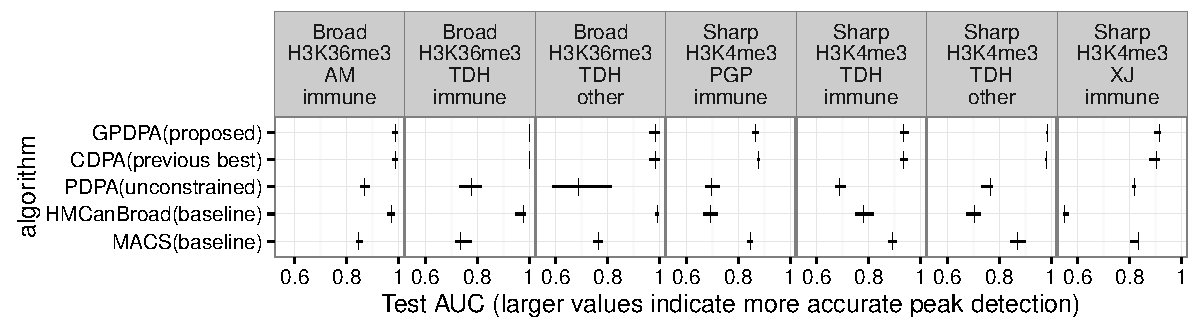
\includegraphics[width=\textwidth]{figure-test-error-dots}
  \vskip -0.5cm
  \caption{Four-fold cross-validation was used to estimate prediction
    accuracy of each algorithm (one panel for each of 7 ChIP-seq data sets). 
Each black circle shows the test AUC in one of four
    cross-validation folds, the shaded grey circle is the mean, and
    the vertical line shows the maximum mean in each data set. It is
    clear that the proposed GPDPA is
    just as accurate as the previous state-of-the-art CDPA, and both are
    more accurate than the other baseline methods. 
% Interactive version
%     available at
%     \url{http://bl.ocks.org/tdhock/raw/886575874144c3b172ce6b7d7d770b9f/}
  }
  \label{fig:test-error-dots}
\end{figure*}

In this section, we show that our proposed GPDPA can be used to
overcome this speed drawback, while maintaining state-of-the-art
accuracy. To show the importance of enforcing the up-down constraint,
we consider the unconstrained Pruned Dynamic Programming Algorithm
(PDPA) of \citet{pruned-dp} as a baseline
(Table~\ref{tab:contribution}). We also compare against two popular
heuristics from the bioinformatics literature, in order to demonstrate
that constrained optimization algorithms such as the CDPA and GPDPA
are more accurate.

% \begin{description}
% \item[Segmentor3IsBack::Segmentor] is an implementation of a
%   functional pruning algorithm for computing the solution to the
%   Segment Neighborhood (\ref{eq:optimal_segment_neighborhood}) problem
%   \citep{Segmentor}. Its average time complexity is $O(n \log n)$,
%   and the solution may or may not obey the up-down constraints on
%   segment means. If it does not, then the model is not directly
%   interpretable in terms of peaks (segments after up changes) and
%   background (segments after down changes), so we discard the model.
% \item[PeakSegDP::cDPA] implements a heuristic algorithm with $O(n^2)$
%   time complexity which attempts to solve the up-down
%   constrained problem \citep{HOCKING-PeakSeg}. Models computed by this
%   algorithm are guaranteed to satisfy the up-down constraint, but may
%   not be the optimal solution to the up-down constrained problem
%   (\ref{eq:min_PeakSeg}).
% \item[coseg::PeakSegPDPA] is our proposed solver for the PeakSeg
%   problem, described in Section~\ref{sec:PeakSeg}. It recovers the
%   optimal solution to the up-down constrained problem
%   (\ref{eq:min_PeakSeg}).  Since Definition~\ref{def:U} contains
%   non-strict inequality constraints, the optimal solution may include
%   adjacent segments with equal mean values. In that case, the model is
%   not directly interpretable in terms of peaks and background, so we
%   discard the model. We expected the speed of the algorithm to be
%   consistent with the $O(n\log n)$ time complexity of other functional
%   pruning algorithms such as Segmentor.
% \item[MACS] is a heuristic algorithm with unknown time complexity from
%   the bioinformatics literature \citep{MACS}. We consider it as a
%   baseline, since it has been shown to achieve state-of-the-art peak
%   detection accuracy for sharp H3K4me3 histone mark data
%   \citep{HOCKING-PeakSeg}.
% \item[HMCanBroad] is a another heuristic algorithm with unknown time
%   complexity \citep{HMCan}. We consider it as a baseline, since it has
%   been shown to achieve state-of-the-art peak detection accuracy for
%   broad H3K36me3 histone mark data \citep{HOCKING-PeakSeg}.
% \end{description}

% We ran each algorithm on the McGill ChIP-seq benchmark data sets
% \citep{HOCKING2016-chipseq}. We begin by comparing the speed,
% feasibility, and optimality of the three optimization-based
% implementations (Segmentor, PeakSegDP, coseg).

\subsection{Empirical time complexity in ChIP-seq data}
\label{sec:results_time}

The ChIP-seq benchmark consists of seven labeled histone data
sets.
% \citep{HOCKING2016-chipseq}. 
Overall there are 2752 count data vectors $\mathbf y_i$ to segment,
varying in size from $n=87$ to $n=263169$ data. For each count data
vector $\mathbf y_i$, we ran each algorithm (CDPA, PDPA, GDPDA) with a
maximum of $K=19$ segments. This implies a maximum of 9 peaks (one for
each even-numbered segment), which is more than enough in these
relatively small data sets. To analyze the empirical time complexity,
we recorded the number of intervals stored in the $\FCC_{k,t}$ cost
functions (Section~\ref{sec:algorithms}), as well as the computation
time in seconds.

% TODO: define I?
As in the PDPA, the time complexity of our proposed GPDPA is
$O(K n I)$, which depends on the number of intervals $I$ (candidate
changepoints) stored in the $\FCC_{k,t}$ cost functions
\citep{pruned-dp-new}. We observed that the number of intervals stored
by the GPDPA increases as a sub-linear function of the number of data
points $n$ (left of Figure~\ref{fig:timings}). For the largest data
set ($n=263169$), the algorithm only stored median=16 and maximum=43
intervals. The most intervals stored was 253 for one data set with
$n=7776$. These results suggest that our proposed GPDPA only stores on
average $O(\log n)$ intervals (possible changepoints), as in the
original PDPA. The overall empirical time complexity is thus
$O(K n \log n)$ for $K$ segments and $n$ data points.

We recorded the timings of each algorithm for computing models with up
to $K=19$ segments (a total of 10 peak models $k\in\{1,3,\dots,19\}$,
from 0 to 9 peaks). Since $K$ is constant, the expected time
complexity was $O(n^2)$ for the CDPA and $O(n \log n)$ for the PDPA
and GPDPA. In agreement with these expectations, our proposed GPDPA
shows $O(n\log n)$ asymptotic timings similar to the PDPA (right of
Figure~\ref{fig:timings}). 

It is clear that the $O(n^2)$ CDPA algorithm is slower than the other
two algorithms, especially for larger data sets. For the largest count
data vector ($n=263169$), the CDPA took over two hours, but the GPDPA
took only
% H3K36me3_TDH_immune        3 McGill0001  146.680 263169
% chr10:18761902-22380580
about two minutes. Our proposed GPDPA is nearly as fast as MACS
\citep{MACS}, a heuristic algorithm from the bioinformatics literature
which took about 1 minute to compute 10 peak models for this data set.

The total computation time to process all 2752 count data vectors was
156 hours for the CDPA, and only 6 hours for the GPDPA (26 times
faster). Overall, these results suggest that our proposed GPDPA enjoys
$O(n\log n)$ time complexity in ChIP-seq data, which makes it possible
to use for very large data sets.



% \subsection{Feasibility and optimality in ChIP-seq data}

% For each of 2752 segmentation problems, we attempt to compute models
% with 0, ..., 9 peaks, so there are a total of 27520 possible models
% for each optimization-based algorithm (Segmentor, PeakSegDP,
% coseg). However, none of the algorithms is theoretically guaranteed to
% return a model which is feasible for the up-down constraint (PeakSegDP
% either recovers an up-down model or no model at all; when coseg and
% Segmentor recovered models that did not obey the PeakSeg up-down
% constraints, we discarded those infeasible models). In this section,
% we compare the algorithms in terms of how frequently they recover
% models which are feasible and optimal.

% % We show the number of models which are feasible for the PeakSeg
% % up-down constraint in Table~\ref{tab:min-train-error}. 
% The PeakSegDP package computed the most feasible models
% (27469/27520=99.8\%), followed by the coseg package
% (21278/27520=77.3\%), and the Segmentor package computed the fewest
% (8106/27520=29.4\%). In terms of optimality, the cDPA (PeakSegDP R
% pkg) computes a sub-optimal model for 7246/27520 = 26.3\% of
% models. For 1032/7246 of these, the PeakSeg solution exists and is
% recovered by our new algo (coseg R pkg) but not the unconstrained algo
% (Segmentor R pkg). These results suggest that in ChIP-seq data sets,
% the new coseg algorithm is more accurate than PeakSegDP, in terms of
% the Poisson likelihood. Furthermore, these results suggest that coseg
% is more useful than Segmentor, since there are many cases for which
% Segmentor does not recover a model that verifies the up-down
% constraint on the segment means.
% Numbers come from figure-PDPA-cDPA-compare.R

% \subsection{Minimum train error in ChIP-seq data}

% We quantified the minimum train error for each optimal segmentation
% algorithm for each of the 2752 problems, by selecting the number of
% peaks $p\in\{0, ..., 9\}$ which had the minimum number of incorrect
% labels (total error = false positives + false negatives). As suggested
% by \citet{HOCKING2016-chipseq}, the baseline MACS algorithm was
% trained by varying the qvalue parameter between 0 and 0.8, and the
% baseline HMCanBroad algorithm was trained by varying the
% finalThreshold parameter between $10^{-10}$ and $10^5$.

% The minimum train error for each algorithm is shown in
% Table~\ref{tab:min-train-error}. The algorithm with the smallest
% minimum train error was PeakSegDP (677/12826=5.3\%), followed by coseg
% (789/12826=6.2\%). The other algorithms had much larger minimum train
% error rates (10.1\%--21.7\%). These results suggest that the new coseg
% algorithm can find segmentation models which are nearly as accurate as
% the previous state-of-the-art PeakSegDP method.


\subsection{Test accuracy in ChIP-seq data}

% To compare the accuracy of the algorithms in the benchmark data sets,
% we computed false negative and false positive rates using labels
% that indicate presence or absence of peaks in specific samples and
% genomic regions \citep{HOCKING2016-chipseq}. Briefly, a false negative
% occurs when no peak is predicted in a region with a positive label,
% and a false positive occurs when a peak is predicted in a region with
% a negative label.  
% We performed 4-fold cross-validation to
% estimate the test error of each algorithm. For each of the 7 data
% sets, we randomly assigned labeled data to one of four folds. For each
% fold, we treat it as a test set, and train a model using all other
% folds.

For the optimal changepoint detection algorithms (CDPA, PDPA, GPDPA),
the prediction problem simplifies to selecting the number of segments
$K_i\in \{1, 3,\dots, 19\}$ for each data vector $i$, resulting in a
predicted peak vector $c^{K_i}(\mathbf y_i)\in\{0,1\}^n$. We select the
number of segments using an oracle penalty
$K_i^\lambda=\argmin_k l_{ik} + \lambda o_{ik}$
\citep{cleynen2013segmentation}, where $l_{ik}$ is the Poisson loss and
$o_{ik}$ is the oracle model complexity for the model with $k$
segments for data vector $i$. 
The learning problem thus simplifies to learning a scalar
penalty constant $\lambda$,
\begin{equation}
  \label{eq:learn-lambda}
  \minimize_{\lambda}
  \sum_{i=1}^m E\left[
    c^{K_i^\lambda}(\mathbf y_i), 
    L_i\right].
\end{equation}

% Multi-parameter affine penalty functions could further increase prediction
% accuracy \citep{HOCKING-penalties}, but we observed that learning a
% single penalty constant is sufficient for state-of-the-art accuracy in
% these data sets (Figure~\ref{fig:test-error-dots}). 

% Furthermore, we wanted to perform a fair comparison with the following
% two baselines from the bioinformatics literature, which also learn
% only one parameter.
To demonstrate that constrained optimal segmentation is more accurate
than typical unsupervised heuristics from the bioinformatics
literature, we also computed test AUC for the MACS and HMCanBroad
algorithms \citep{MACS, HMCan}. MACS is a popular heuristic for data
with a sharp peak pattern such as H3K4me3, and \mbox{HMCanBroad} is a
popular heuristic for data with a broad peak pattern such as
H3K36me3. Although these algorithms are not designed for supervised
learning, we trained them by performing grid search over a single
significance threshold parameter (qvalue for MACS and finalThreshold
for HMCanBroad).
% Note that since these are not changepoint detection algorithms,
% there is no parameter for we did not use these algorithms in the
% speed comparison
% Without this training step, the unsupervised default parameters of
% these algorithms yield high false positive rates.


In each of the seven data sets in the histone benchmark,
%\citep{HOCKING2016-chipseq}, 
we performed four-fold cross-validation and computed test AUC to
estimate the accuracy of each algorithm. The previous algorithm with
state-of-the-art accuracy on this benchmark was the CDPA, which
enforces the up-down constraint on segment means. We expected our
proposed GPDPA to perform just as well, since it also enforces that
constraint. In agreement with our expectation, we observed that the
CDPA and GPDPA yield comparable test AUC in all seven data sets
(Figure~\ref{fig:test-error-dots}). In contrast, the unconstrained
PDPA had much lower test AUC in several data sets, because of lower
true positive rates. These results provide convincing
evidence that the constraint is necessary for optimal peak detection
accuracy.

Since the baseline HMCanBroad algorithm was designed for data with a
broad peak pattern, we expected it to perform well in the H3K36me3
data. In agreement with this expectation, HMCanBroad showed
state-of-the-art test AUC in two H3K36me3 data sets (broad peak
pattern), but was very inaccurate in four H3K4me3 data sets (sharp
peak pattern). We expected the baseline MACS algorithm to perform well
in the H3K4me3 data sets, since it was designed for data with a sharp
peak pattern. In contrast to this expectation, MACS had test AUC
values much lower than the optimization-based algorithms in all seven
data sets (Figure~\ref{fig:test-error-dots}). These results suggest
that constrained optimal changepoint detection algorithms are more
accurate than the heuristics from the bioinformatics literature.


% \begin{table}[b!]
%   \centering
%   % latex table generated in R 3.3.3 by xtable 1.7-4 package
% Wed Jun 21 17:03:48 2017
\begin{tabular}{rrrrr}
  \hline
 & errors & fp & fn & feasible models \\ 
  \hline
CDPA & 677 & 116 & 561 & 27469 \\ 
  GPDPA & 789 & 94 & 695 & 21278 \\ 
  macs & 1293 & 519 & 774 &  \\ 
  PDPA & 1544 & 46 & 1498 & 8106 \\ 
  hmcan.broad & 2778 & 367 & 2411 &  \\ 
  \hline possible & 12826 & 11037 & 7225 & 27520 \\ 
   \hline
\end{tabular}

%   \caption{Comparison of algorithms in the ChIP-seq data sets,
%     in terms of minimum train error and number of feasible models. 
%     For each of the 2752 separate segmentation problems, 
%     each algorithm was run with several parameter values (see text for details), 
%     and we selected the parameter with the minimum number of incorrect labels
%     (errors = fp + fn). 
%     The new algorithm implemented in the coseg R package 
%     commits fewer false positives than the slower PeakSegDP heuristic, 
%     and fewer errors than the other baseline methods.
%     The new algorithm computed models that are feasible for the PeakSeg up-down constraint
%     more frequently than the unconstrained Segmentor algo,
%     but less frequently than the PeakSegDP algo.}
%   \label{tab:min-train-error}
% \end{table}

\section{Discussion and conclusions}
\label{sec:discussion}

Algorithms for changepoint detection can be classified in terms of
time complexity, optimality, constraints, and pruning techniques
(Table~1). In this paper, we investigated generalizing the functional
pruning technique originally discovered by \citet{pruned-dp} and
\citet{johnson}. We showed that the functional pruning technique can
be used to compute optimal changepoints subject to affine constraints
on adjacent segment mean parameters.

We showed that our proposed Generalized Pruned Dynamic Programming
Algorithm (GPDPA) enjoys the same log-linear $O(Kn\log n)$ time
complexity as the original unconstrained PDPA, when applied to peak
detection in ChIP-seq data sets (Figure~\ref{fig:timings}). However,
we observed that the up-down constrained GPDPA is much more accurate
than the unconstrained PDPA (Figure~\ref{fig:test-error-dots}). These
results suggest that the up-down constraint is necessary for computing
a changepoint model with optimal peak detection accuracy. Indeed, we
observed that the GPDPA enjoys the same state-of-the-art accuracy as
the previous best, the relatively slow quadratic $O(Kn^2)$ time
CDPA.

We observed that the heuristic algorithms which are
popular in the bioinformatics literature (MACS, HMCanBroad) are much
less accurate than the optimal changepoint detection algorithms (CDPA,
PDPA, GPDPA). In the past these sub-optimal heuristics have been
preferred because of their speed. For example, the CDPA took 2 hours
to compute 10 peak models in the largest data set in the ChIP-seq
benchmark, whereas the GPDPA took 2 minutes, and the MACS heuristic
took 1 minute. Using our proposed GPDPA, it is now possible to compute
highly accurate models in an amount of time that is comparable to
heuristic algorithms. For large data sets where accuracy is essential,
our proposed GPDPA can now be used as an optimal alternative to
heuristic algorithms.

For future work we will be interested in exploring pruning techniques
for other constrained changepoint models. When the number of expected
changepoints grows with the number of data points, then $K=O(n)$ and
our proposed GPDPA has $O(n^2 \log n)$ average time complexity (since
it computes all models with $1,\dots,K$ segments). We have already
started modifying the GPDPA for optimal partitioning
\citep{optimal-partitioning}, which computes the $K$-segment model for
a single penalty constant $\lambda$ (without computing models with
$1,\dots,K-1$ segments) in $O(n\log n)$ time. We have not yet found a
way to use the inequality pruning technique of \citet{pelt} for
constrained changepoint models. This will be an interesting direction
for future research, since inequality pruning is easier to implement
than functional pruning \citep{fpop}.

\bibliographystyle{icml2016}
\newpage
\bibliography{refs-abbrev}

\end{document} 
